% 高一102_华师大二附中_周末作业5.tex
%   —— 高一上数学“2026-2027 年华师大二附中高一上周末作业 5”（试卷版/答案版）
% 试卷版：xelatex 高一102_华师大二附中_周末作业5.tex
% 答案版：xelatex "\def\isanswer{1}% 高一102_华师大二附中_周末作业5.tex
%   —— 高一上数学“2026-2027 年华师大二附中高一上周末作业 5”（试卷版/答案版）
% 试卷版：xelatex 高一102_华师大二附中_周末作业5.tex
% 答案版：xelatex "\def\isanswer{1}% 高一102_华师大二附中_周末作业5.tex
%   —— 高一上数学“2026-2027 年华师大二附中高一上周末作业 5”（试卷版/答案版）
% 试卷版：xelatex 高一102_华师大二附中_周末作业5.tex
% 答案版：xelatex "\def\isanswer{1}% 高一102_华师大二附中_周末作业5.tex
%   —— 高一上数学“2026-2027 年华师大二附中高一上周末作业 5”（试卷版/答案版）
% 试卷版：xelatex 高一102_华师大二附中_周末作业5.tex
% 答案版：xelatex "\def\isanswer{1}\input{高一102_华师大二附中_周末作业5.tex}"
% 紧凑版：xelatex "\def\iscompact{1}\input{高一102_华师大二附中_周末作业5.tex}"
%
% 原始材料：微信公众号“魔都数学加油站”文章，作者破晓，2026-11-01 21:56 发布；
% 连载“27学年高一102”，原文标题“27学年高一102——2026-2027年上海市华师大二附中高一上周末作业5函数”；
% 原文链接：https://mp.weixin.qq.com/s/CDvOCcxFskIe9aFUeKi3Ww。
% 正文为 13 张 PNG 页（第 1、2、10、13 页 2560×3620，其余 4762×6735），题目下印有【解析】，为讲评版。
% 题目、解析均据原图转录；卷面水印及公众号页脚未录入。
%
% 卷首标题：原卷印作“2026-2027 年华师大二附中高一上周末作业 5”（公众号标题中的“上海市”“函数”
% 卷面标题行没有，本稿照卷面），年份区间按全稿惯例排 en dash；原卷未印副标题，本稿按题目内容
% 标为“函数”（全稿首份以函数为单一模块的卷子）。
%
% 与原卷的排版差异：
%   ① 原文从第 3 题起，填空题编号为 3—12、选择题为 13—16、解答题为 17—21，本稿保留原题号；
%   ② 原卷每题下直接印【解析】，本稿按全稿惯例将解析置于答案版；选择题括号内未印答案，另由
%      解析末句“故选 X”给出；
%   ③ 原卷未印副标题，本稿按“知识模块”口径补出；
%   ④ 原卷填空横线按全稿惯例排为 \blankline[4.4em]；解答题按惯例加 \ansspace；选择题括号排
%      \mbox{（\quad）}、选项段前按惯例加 \keepwithprev；
%   ⑤ 原卷 $f(x)_{min}$、$f(x)_{max}$ 等下标排斜体，按 高一96 成例改正体 $\min$、$\max$；
%   ⑥ 原卷数集排斜体 $R$（第 13 题排粗体），按全稿惯例改 $\R$；
%   ⑦ 第 7、10 两题的解析插图裁自原图（去粉色水印转灰度），仅答案版显示。
%
% 原卷存疑／笔误（均照录加注）：
%   第 3 题解析“减去都对应 −2 和 2 的”措辞含糊（意为减去恒取 −2 与恒取 2 的两个常函数）；
%   第 15 题解析“其最小值趋向于 f(−1) 即 2”（该段 f(x)=x²+x+2 在 x→−1⁻ 时趋于 2、取不到）；
%   第 16 题解析末句“因此只有当 x=√3/2”（按上下文应为 f(1)=√3/2）；
%   第 16 题解析以 f(1)=√3、√3/3、0 赋值时称“得到的圆心角为 π/3、π/6、0”，其中 √3/3 对应
%   圆心角 π/6 的说法与该点 (1,√3/3) 的实际幅角一致，但与选项 C（√3/3）被排除的结论矛盾
%   （幅角 π/6 的点旋转 π/6 后落到幅角 π/3 处，仍占 12 等分点位，原卷解析未展开），照录。
%
% 行数核对：逐题数 \step/\stepm 条数，合计 155 条（Q3：2；Q4：3；Q5：6；Q6：5；Q7：19；
% Q8：2；Q9：4；Q10：5；Q11：3；Q12：19；Q13：2；Q14：5；Q15：8；Q16：5；Q17：10；
% Q18：6；Q19：10；Q20：13；Q21：28），与原卷印刷行逐题相等。
%
\documentclass[a4paper,11pt]{article}
\usepackage{common}

\begin{document}

\examtitlest[3]{2026--2027 年华师大二附中高一上周末作业 5}{函数}

\bigsec{一、填空题}

\begin{enumerate}
\setcounter{enumi}{2}

\item 已知函数 $y=f(x)$ 的定义域为 $\{-2,-1,1,2\}$，值域为 $\{-2,2\}$，则满足条件的函数
$y=f(x)$ 最多有\blankline[4.4em]个.

\ifanswer
\solbegin
\step{定义域中 4 个元素每个都可以对应 $-2$ 和 $2$ 中的一个，减去都对应 $-2$ 和 $2$ 的，}
\step{则满足条件的函数 $y=f(x)$ 最多有 $2^4-2=14$.}
\solend

\fi

\item 已知函数 $f(2x)$ 的定义域为 $[-2,2]$，则函数 $f(x-3)$ 的定义域为\blankline[4.4em].

\ifanswer
\solbegin
\step{因为函数 $f(2x)$ 的定义域为 $[-2,2]$，即 $-2\leqslant x\leqslant2$，所以 $-4\leqslant2x\leqslant4$，}
\step{得 $f(x)$ 的定义域为 $[-4,4]$，由 $-4\leqslant x-3\leqslant4$，解得 $-1\leqslant x\leqslant7$，}
\step{即函数 $f(x-3)$ 的定义域为 $[-1,7]$.}
\solend

\fi

\item 函数 $f(x)=\begin{cases}-x-1, & x<0\\ -x+1, & x>0\end{cases}$，则 $f(x)-f(-x)>1$ 的解集为\blankline[4.4em].

\ifanswer
\solbegin
\step{定义域为 $\{x\mid x\neq0\}$.}
\step{当 $x<0$ 时，$-x>0,f(-x)=x+1$，}
\step{$f(x)-f(-x)=(-x-1)-(x+1)=-2x-2>1$，得 $x<-\dfrac32$.}
\step{当 $x>0$ 时，$f(-x)=x-1,f(x)-f(-x)=(-x+1)-(x-1)=-2x+2>1$，}
\step{得 $0<x<\dfrac12$.}
\step{故解集为 $\left(-\infty,-\dfrac32\right)\cup\left(0,\dfrac12\right)$.}
\solend

\fi

\item 已知函数 $f(x)=x^2-2(m-3)x+5$ 在区间 $[2,+\infty)$ 上的最小值为 1，则实数 $m=$\blankline[4.4em].

\ifanswer
\solbegin
\step{函数 $f(x)$ 图象的对称轴为 $x=m-3$.}
\step{当 $m-3\leqslant2$，即 $m\leqslant5$ 时，$f(x)_{\min}=f(2)=9-4m+12=1$，解得 $m=5$；}
\step{当 $m-3>2$，即 $m>5$ 时，$f(x)_{\min}=f(m-3)=-m^2+6m-4=1$，}
\step{解得 $m=5$（舍去）或 $1$（舍去），}
\step{综上，$m=5$.}
\solend

\fi

\item 已知函数 $f(x)=\begin{cases}x^2-2x, & x\leqslant m\\ -\dfrac23x, & x>m\end{cases}$ 的值域为 $R$，则实数 $m$ 的取值范围是\blankline[4.4em].

\ifanswer
\solbegin
\step{对于函数 $y_1=x^2-2x$，则 $y_1=(x-1)^2-1\geqslant-1$，当且仅当 $x=1$ 时取等号，}
\step{且函数在 $(-\infty,1)$ 上严格减，在 $(1,+\infty)$ 上严格增，}
\step{对于函数 $y_2=-\dfrac23x$，令 $y_2=-1$，则 $x=\dfrac32$，且函数在定义域上严格减，}
\step{令 $x^2-2x=-\dfrac23x$，解得 $x=0$ 或 $x=\dfrac43$，}
\step{所以 $y_2=-\dfrac23x$ 与 $y_1=x^2-2x$ 的两个交点分别为 $(0,0)$、$\left(\dfrac43,-\dfrac89\right)$，}
\step{则函数 $y_2=-\dfrac23x$ 与 $y_1=x^2-2x$ 的图象如图所示：}
\begin{center}
% 原图第 2 页解析插图直接裁取（原卷排于解析行右侧）。
% 裁框取图形区域，已去粉色水印转灰度。
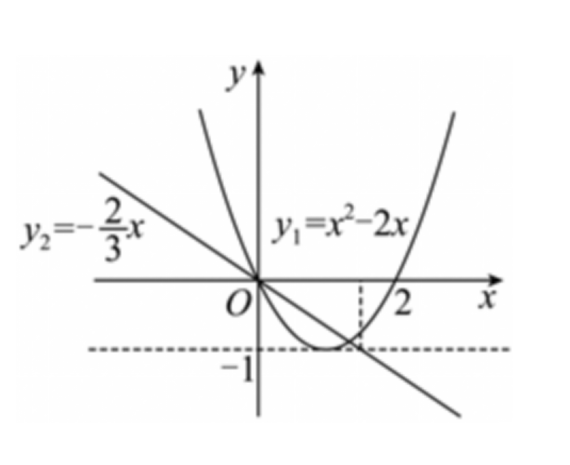
\includegraphics[width=0.24\textwidth]{figures/gao102_q7.png}
\end{center}
\step{当 $m>\dfrac32$ 时，当 $x>m$ 时 $f(x)\in\left(-\infty,-\dfrac23m\right)$，当 $x\leqslant m$ 时 $f(x)\in[-1,+\infty)$，}
\step{显然 $-\dfrac23m<-1$，此时函数 $f(x)$ 的值域不为 $R$，不符合题意；}
\step{当 $m<0$ 时，当 $x>m$ 时，$f(x)\in\left(-\infty,-\dfrac23m\right)$，}
\step{当 $x\leqslant m$ 时，$f(x)\in[m^2-2m,+\infty)$，}
\step{此时 $m^2-2m-\left(-\dfrac23m\right)=m^2-\dfrac43m=m\left(m-\dfrac43\right)>0$，即 $m^2-2m>-\dfrac23m$，}
\step{此时函数 $f(x)$ 的值域不为 $R$，不符合题意；}
\step{当 $0\leqslant m\leqslant\dfrac43$ 时，在 $x\in(0,m)$ 时 $y_2>y_1$，即 $m^2-2m<-\dfrac23m$，}
\step{此时 $f(x)$ 的值域为 $R$，符合题意，}
\step{当 $\dfrac43<m\leqslant\dfrac32$ 时，当 $x>m$ 时，$f(x)\in\left(-\infty,-\dfrac23m\right)$，}
\step{当 $x\leqslant m$ 时，$f(x)\in[-1,+\infty)$，}
\step{此时 $-1-\left(-\dfrac23m\right)=\dfrac23m-1\leqslant0$，即 $-1\leqslant-\dfrac23m$，}
\step{此时函数 $f(x)$ 的值域为 $R$，符合题意；}
\step{综上，$0\leqslant m\leqslant\dfrac32$，即实数 $m$ 的取值范围是 $\left[0,\dfrac32\right]$.}
\solend

\fi

\item 已知函数 $f(x)=x^2-2ax+b$（$a>1$）的定义域和值域都为 $[1,a]$，则 $b=$\blankline[4.4em].

\ifanswer
\solbegin
\step{$f(x)=x^2-2ax+b$（$a>1$）在 $[1,a]$ 严格减，}
\step{则 $f(1)=1-2a+b=a,f(a)=-a^2+b=1$，解得 $a=2,b=5$，所以 $b=5$.}
\solend

\fi

\item 若 $f(x)$ 满足 $f(x+y)=f(x)f(y)$，当 $x>0$ 时，$f(x)$ 的值域为 $(1,+\infty)$，则 $x<0$ 时，
$f(x)$ 的取值范围为\blankline[4.4em].

\ifanswer
\solbegin
\step{因为 $f(x+y)=f(x)f(y)$，令 $x=1$，$y=0$，得 $f(1+0)=f(1)f(0)$，}
\step{又因为当 $x>0$ 时，$f(x)>1$，所以 $f(1)>1>0$，故 $f(0)=1$.}
\step{当 $x<0$ 时，$-x>0$，令 $y=-x$，得 $f(x-x)=f(0)=1=f(x)f(-x)$，}
\step{故 $f(x)=\dfrac1{f(-x)}\in(0,1)$，故 $x<0$ 时，$f(x)$ 的取值范围为 $(0,1)$.}
\solend

\fi

\item 设函数 $f(x)=\begin{cases}x^2+x, & x<0\\ -x^2, & x\geqslant0\end{cases}$，若 $f(f(a))\leqslant2$，则实数 $a$ 的取值范围是\blankline[4.4em].

\ifanswer
\solbegin
\step{函数 $f(x)=\begin{cases}x^2+x, & x<0\\ -x^2, & x\geqslant0\end{cases}$，它的图象如图所示：}
\begin{center}
% 原图第 4 页解析插图直接裁取（原卷排于解析行右侧）。
% 裁框取图形区域，已去粉色水印转灰度。
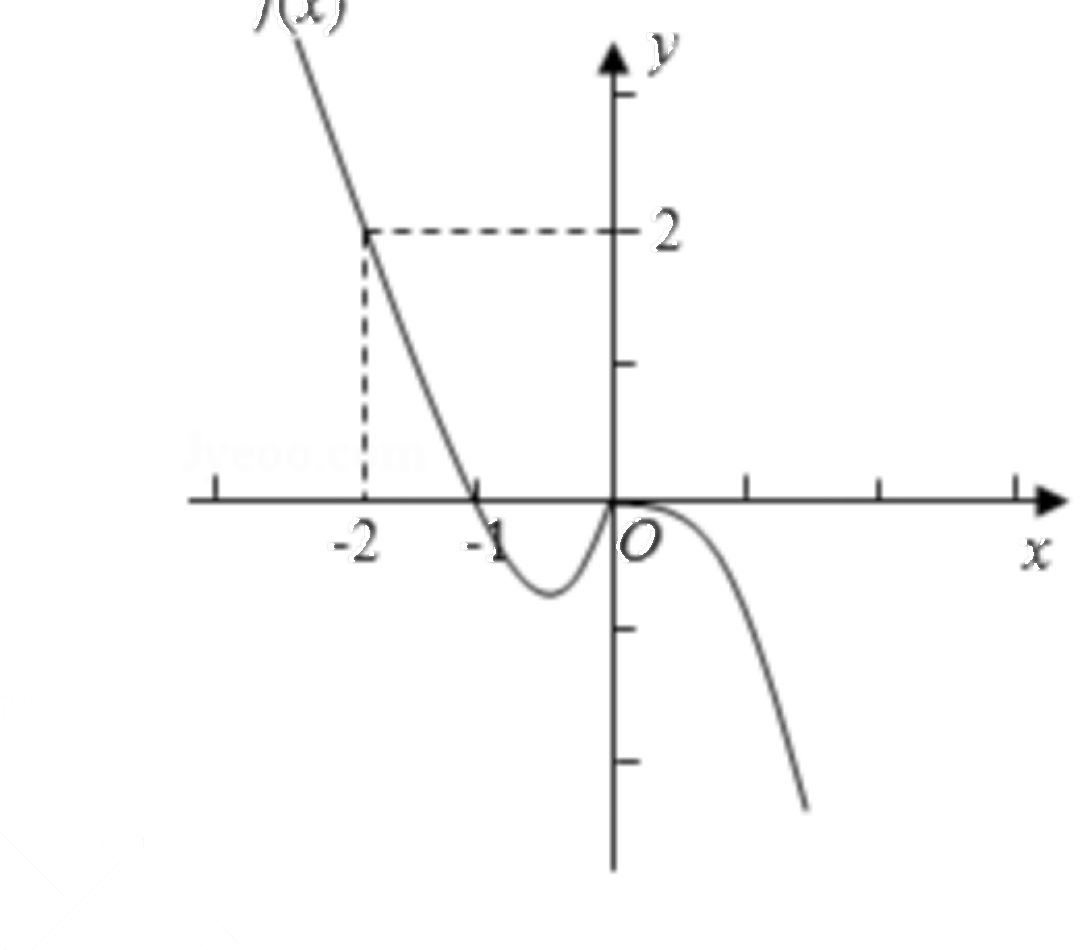
\includegraphics[width=0.30\textwidth]{figures/gao102_q10.png}
\end{center}
\step{由 $f(f(a))\leqslant2$，得 $f(a)\geqslant-2$.}
\step{当 $a<0$ 时，$f(a)=a^2+a=\left(a+\dfrac12\right)^2-\dfrac14\geqslant-2$ 恒成立；}
\step{当 $a\geqslant0$ 时，$f(a)=-a^2\geqslant-2$，即 $a^2\leqslant2$，解得 $0\leqslant a\leqslant\sqrt2$，}
\step{则实数 $a$ 的取值范围是 $(-\infty,\sqrt2]$.}
\solend

\fi

\item 已知二次函数 $f(x)$、$g(x)$ 的二次项系数均为 1，且满足
$\dfrac{f(2025)}{g(2025)}=\dfrac{f(2026)}{g(2026)}=\dfrac{2026}{2025}$，
则 $2026g(2027)-2025f(2027)$ 的值为\blankline[4.4em].

\ifanswer
\solbegin
\step{令 $h(x)=2026g(x)-2025f(x)$，其二次项系数为 $2026-2025=1$.}
\step{由比例条件得 $h(2025)=h(2026)=0$，}
\step{因此 $h(x)=(x-2025)(x-2026),h(2027)=2\times1=2$.}
\solend

\fi

\item 已知函数 $f(x)=\left\lvert x+\dfrac1x-a\right\rvert+1$，对任意实数 $x_1$、$x_2$、$x_3\in\left[\dfrac13,3\right]$，使得以
$f(x_1)$、$f(x_2)$、$f(x_3)$ 数值为边长可构成三角形，则实数 $a$ 的取值范围为\blankline[4.4em].

\ifanswer
\solbegin
\step{对任意实数 $x_1,x_2,x_3\in\left[\dfrac13,3\right]$，}
\step{使得以 $f(x_1)$、$f(x_2)$、$f(x_3)$ 数值为边长可构成三角形，}
\step{只需 $2f(x)_{\min}>f(x)_{\max}$，设 $g(x)=x+\dfrac1x-a$，}
\step{当 $x\in\left[\dfrac13,1\right)$ 时，函数 $g(x)$ 严格减，当 $x\in(1,3]$ 时，函数 $g(x)$ 严格增，}
\step{因为 $g(1)=2-a,g(3)=\dfrac{10}3-a,g\left(\dfrac13\right)=\dfrac{10}3-a$，所以 $g(x)\in\left[2-a,\dfrac{10}3-a\right]$，}
\step{当 $2-a\geqslant0$ 时，即 $a\leqslant2$ 时，$f(x)=\left\lvert x+\dfrac1x-a\right\rvert+1=g(x)+1$，}
\step{此时 $f(x)\in\left[3-a,\dfrac{13}3-a\right]$，}
\step{因此由 $2f(x)_{\min}>f(x)_{\max}\Rightarrow2(3-a)>\dfrac{13}3-a\Rightarrow a<\dfrac53$，而 $a\leqslant2$，所以 $a<\dfrac53$；}
\step{当 $\dfrac{10}3-a\leqslant0$，即 $a\geqslant\dfrac{10}3$ 时，$f(x)=\left\lvert x+\dfrac1x-a\right\rvert+1=-g(x)+1$，}
\step{此时 $f(x)\in\left[a-\dfrac73,a-1\right]$，}
\step{因此由 $2f(x)_{\min}>f(x)_{\max}\Rightarrow2\left(a-\dfrac73\right)>a-1\Rightarrow a>\dfrac{11}3$，而 $a\geqslant\dfrac{10}3$，所以 $a>\dfrac{11}3$，}
\step{若 $2-a<0<\dfrac{10}3-a$ 时，即 $2<a<\dfrac{10}3$ 时，}
\step{若 $a-2\geqslant\dfrac{10}3-a\Rightarrow a\geqslant\dfrac83$，即当 $\dfrac83\leqslant a<\dfrac{10}3$ 时，}
\step{显然此时 $f(x)_{\min}=1$，$f(x)_{\max}=a-2+1=a-1$，}
\step{由 $2f(x)_{\min}>f(x)_{\max}\Rightarrow2\times1>a-1\Rightarrow a<3$，显然 $\dfrac83\leqslant a<3$，}
\step{若 $a-2<\dfrac{10}3-a\Rightarrow a<\dfrac83$，即当 $2<a<\dfrac83$ 时，}
\step{显然此时 $f(x)_{\min}=1,f(x)_{\max}=\dfrac{10}3-a+1=\dfrac{13}3-a$，}
\step{因此由 $2f(x)_{\min}>f(x)_{\max}\Rightarrow2\times1>\dfrac{13}3-a\Rightarrow a>\dfrac73$，而 $\dfrac73<a<\dfrac83$，}
\step{综上，实数 $a$ 的取值范围为 $\left(-\infty,\dfrac53\right)\cup\left(\dfrac73,3\right)\cup\left(\dfrac{11}3,+\infty\right)$.}
\solend

\fi

\end{enumerate}

\bigsec{二、选择题}

\begin{enumerate}
\setcounter{enumi}{12}

\item 已知 $f(x)$ 是定义在 $\R$ 上的奇函数，$g(x)$ 是定义在 $\R$ 上的偶函数，则\mbox{（\quad）}

\keepwithprev
A. $f(x)g(x)$ 是偶函数\qquad B. $f(g(x))$ 是奇函数

C. $f(x)-g(x)$ 是奇函数\qquad D. $g(f(x))$ 是偶函数

\ifanswer
\solbegin
\step{$g(f(x))$ 的定义域为 $\R$，且 $g(f(-x))=g(-f(x))=g(f(x))$，}
\step{所以 $g(f(x))$ 是偶函数，故选 $D$.}
\solend

\fi

\item 已知定义在 $R$ 上的偶函数 $f(x)=\lvert x-m+1\rvert-2$，若正实数 $a$、$b$ 满足 $f(a)+f(2b)=m$，
则 $\dfrac1a+\dfrac2b$ 的最小值为\mbox{（\quad）}

\keepwithprev
A. $\dfrac95$\qquad\qquad B. $9$\qquad\qquad C. $\dfrac85$\qquad\qquad D. $8$

\ifanswer
\solbegin
\step{因为 $f(x)=\lvert x-m+1\rvert-2$ 是偶函数，所以 $-m+1=0$，所以 $m=1$，}
\step{所以 $f(x)=\lvert x\rvert-2$，若正实数 $a$、$b$ 满足 $f(a)+f(2b)=m$，}
\step{则 $a-2+2b-2=1$，所以 $a+2b=5$，}
\step{所以 $\dfrac1a+\dfrac2b=\dfrac15(a+2b)\left(\dfrac1a+\dfrac2b\right)=\dfrac15\left(5+\dfrac{2a}b+\dfrac{2b}a\right)\geqslant\dfrac95$，}
\step{当且仅当 $a=b=\dfrac53$ 时取等号，则 $\dfrac1a+\dfrac2b$ 的最小值为 $\dfrac95$，故选 $A$.}
\solend

\fi

\item 设函数 $g(x)=x^2-2$（$x\in\R$），$f(x)=\begin{cases}g(x)+x+4, & x<g(x)\\ g(x)-x, & x\geqslant g(x)\end{cases}$，则 $f(x)$ 的值域是

\mbox{（\quad）}

\keepwithprev
A. $\left[-\dfrac94,0\right]\cup(1,+\infty)$\qquad\qquad B. $[0,+\infty)$

C. $\left[-\dfrac94,+\infty\right)$\qquad\qquad D. $\left[-\dfrac94,0\right]\cup(2,+\infty)$

\ifanswer
\solbegin
\step{当 $x<g(x)$，即 $x<x^2-2$，$(x-2)(x+1)>0$ 时，$x>2$ 或 $x<-1$，}
\step{$f(x)=g(x)+x+4=x^2-2+x+4=x^2+x+2=(x+0.5)^2+1.75$，}
\step{其最小值趋向于 $f(-1)$ 即 2，无最大值，}
\step{因此这个区间的值域为 $(2,+\infty)$.}
\step{当 $x\geqslant g(x)$ 时，$-1\leqslant x\leqslant2$，$f(x)=g(x)-x=x^2-2-x=(x-0.5)^2-2.25$，}
\step{其最小值为 $f(0.5)=-2.25$，其最大值为 $f(2)=0$，}
\step{因此这区间的值域为 $[-2.25,0]$.}
\step{综上，函数值域为 $\left[-\dfrac94,0\right]\cup(2,+\infty)$，故选 $D$.}
\solend

\fi

\item 设 $D$ 是含数 1 的有限实数集，$f(x)$ 是定义在 $D$ 上的函数，若 $f(x)$ 的图象绕原点逆时针
旋转 $\dfrac{\pi}{6}$ 与原图象重合，则在以下各项中，$f(1)$ 的可能取值只能是\mbox{（\quad）}

\keepwithprev
A. $\sqrt3$\qquad\qquad B. $\dfrac{\sqrt3}2$\qquad\qquad C. $\dfrac{\sqrt3}3$\qquad\qquad D. $0$

\ifanswer
\solbegin
\step{问题相当于圆上由 12 个点为一组，每次绕原点逆时针旋转 $\dfrac{\pi}{6}$ 个单位后与下一个点}
\step{会重合。我们可以通过代入和赋值的方法，当 $f(1)=\sqrt3$、$\dfrac{\sqrt3}3$、$0$ 时，}
\step{此时得到的圆心角为 $\dfrac{\pi}{3}$、$\dfrac{\pi}{6}$、$0$，然而此时 $x=0$ 或者 $x=1$ 时，}
\step{都有 2 个 $y$ 与之对应，而我们知道函数的定义就是要求一个 $x$ 只能对应一个 $y$，}
\step{因此只有当 $x=\dfrac{\sqrt3}2$，此时旋转 $\dfrac{\pi}{6}$，此时满足一个 $x$ 只会对应一个 $y$，故选 $B$.}
\solend

\fi

\end{enumerate}

\bigsec{三、解答题}

\begin{enumerate}
\setcounter{enumi}{16}

\item 求下列函数的值域.

（1）$y=\dfrac{2x^2-3x+5}{x-1}\left(x\in\left[\dfrac32,3\right]\right)$；

（2）$f(x)=\sqrt{x}-\sqrt{2-x}+\sqrt{x(2-x)}$.

\ansspace*[10]

\ifanswer
\solbegin
\stepm{（1）}{令 $t=x-1$，则 $t\in\left[\dfrac12,2\right]$，原函数化为 $Y(t)=2t+\dfrac4t+1$.}
\step{当 $0<u<v$ 时，$Y(v)-Y(u)=2(v-u)\left(1-\dfrac2{uv}\right)$，}
\step{所以 $Y$ 在 $\left[\dfrac12,\sqrt2\right]$ 上严格递减，在 $[\sqrt2,2]$ 上严格递增.}
\step{由 $Y(\sqrt2)=4\sqrt2+1,Y\left(\dfrac12\right)=10,Y(2)=7$，得值域为 $[4\sqrt2+1,10]$.}
\stepm{（2）}{定义域为 $[0,2]$.}
\step{令 $s=\sqrt{x}-\sqrt{2-x}$，$\sqrt{x}$ 与 $-\sqrt{2-x}$ 均随 $x$ 严格递增，}
\step{$s$ 从 $-\sqrt2$ 递增到 $\sqrt2$，即 $s\in[-\sqrt2,\sqrt2]$.}
\step{由 $s^2=2-2\sqrt{x(2-x)}$，得 $f(x)=s+\dfrac{2-s^2}2=-\dfrac12(s-1)^2+\dfrac32$.}
\step{当 $s=1$ 时取得最大值 $\dfrac32$；当 $s=-\sqrt2$ 时取得最小值 $-\sqrt2$；}
\step{因此值域为 $\left[-\sqrt2,\dfrac32\right]$.}
\solend

\fi

\item 已知 $f(2x+1)=\dfrac{2x+1}{x+1}$.

（1）解不等式 $f(x)<x$；

（2）求 $f(1)+f(2)+\cdots+f(6)+f\left(\dfrac12\right)+f\left(\dfrac13\right)+\cdots+f\left(\dfrac16\right)$ 的值.

\ansspace*[12]

\ifanswer
\solbegin
\step{令 $t=2x+1$，则 $x=\dfrac{t-1}2$，得 $f(t)=\dfrac{2t}{t+1},t\neq-1$.}
\stepm{（1）}{不等式等价于 $\dfrac{2x}{x+1}<x\Leftrightarrow\dfrac{x(x-1)}{x+1}>0$.}
\step{以 $-1,0,1$ 分区间判断符号，得解集为 $(-1,0)\cup(1,+\infty)$.}
\stepm{（2）}{当 $x>0$ 时，$f(x)+f\left(\dfrac1x\right)=\dfrac{2x}{x+1}+\dfrac2{x+1}=2$.}
\step{将 $f(2),\cdots,f(6)$ 分别与其倒数对应的函数值配对，共 5 对，且 $f(1)=1$，}
\step{因此原式$=1+5\times2=11$.}
\solend

\fi

\item 已知函数 $f(x)$、$g(x)$ 是定义在 $R$ 上的函数，其中 $f(x)$ 是奇函数，$g(x)$ 是偶函数，且
$f(x)+g(x)=ax^2-x$.

（1）求 $f(x)$ 和 $g(x)$ 的解析式；

（2）$h(x)=f(x)+g(x)+(1-a)x^2-2ax+4$ 在 $[1,3]$ 上有两个零点，求实数 $a$ 的取值范
围.

\ansspace*[14]

\ifanswer
\solbegin
\stepm{（1）}{因为 $f(x)+g(x)=ax^2-x$①，所以 $f(-x)+g(-x)=ax^2+x$，}
\step{又 $f(x)$ 是奇函数，$g(x)$ 是偶函数，}
\step{所以 $f(-x)=-f(x)$，$g(-x)=g(x)$，}
\step{所以 $-f(x)+g(x)=ax^2+x$②，}
\step{联立①②解得 $f(x)=-x$，$g(x)=ax^2$.}
\stepm{（2）}{$h(x)=f(x)+g(x)+(1-a)x^2-2ax+4$}
\step{$=ax^2-x+(1-a)x^2-2ax+4=x^2-(2a+1)x+4$，}
\step{是开口向上，对称轴为 $x=\dfrac{2a+1}2$ 的二次函数，}
\step{因为 $h(x)$ 在 $[1,3]$ 上有两个零点，所以 $\begin{cases}\Delta=(2a+1)^2-16>0\\ 1<\dfrac{2a+1}2<3\\ h(1)=1-(2a+1)+4\geqslant0\\ h(3)=9-3(2a+1)+4\geqslant0\end{cases}$，}
\step{解得 $\dfrac32<a\leqslant\dfrac53$，故实数 $a$ 的取值范围为 $\left(\dfrac32,\dfrac53\right]$.}
\solend

\fi

\item 若函数 $f(x)$ 在区间 $[a,b]$ 上的值域恰为 $\left[\dfrac1b,\dfrac1a\right]$，则称区间 $[a,b]$ 为 $f(x)$ 的一个“倒域
区间”。已知定义在 $[-4,4]$ 上的奇函数 $g(x)$，当 $x\in[0,4]$ 时，$g(x)=-x^2+2x$.

（1）求 $g(x)$ 的解析式；

（2）若关于 $x$ 的方程 $g(x)=-mx-m$ 在 $(0,4)$ 上恰有两个不相等的实数根，求实数 $m$ 的
取值范围；

（3）求函数 $g(x)$ 在 $[-4,0]$ 内的“倒域区间”.

\ansspace*[16]

\ifanswer
\solbegin
\stepm{（1）}{当 $x\in[-4,0)$ 时，$-x\in(0,4]$，}
\step{由奇函数的定义得 $g(x)=-g(-x)=-[(-x)^2+2(-x)]=x^2+2x$，}
\step{所以 $g(x)=\begin{cases}-x^2+2x, & 0\leqslant x\leqslant4\\ x^2+2x, & -4\leqslant x<0\end{cases}$.}
\stepm{（2）}{方程 $g(x)=-mx-m$，即 $x^2-(m+2)x-m=0$，}
\step{设 $h(x)=x^2-(m+2)x-m$，$0<x<4$，}
\step{由题意得 $\begin{cases}h(0)=-m>0\\ h(4)=8-5m>0\\ \Delta=(m+2)^2+4m>0\\ 0<\dfrac{m+2}2<4\end{cases}$，解得 $2\sqrt3-4<m<0$，}
\step{即实数 $m$ 的取值范围是 $(2\sqrt3-4,0)$.}
\stepm{（3）}{易得当 $-4\leqslant a<b<0$ 时，$\dfrac1b<\dfrac1a$，}
\step{且 $g(x)$ 在 $[-4,-1]$ 上严格减，在 $[-1,0]$ 上严格增，}
\step{故当 $x\in[-4,0]$ 时，$g(x)_{\min}=g(-1)=-1$，}
\step{所以 $\dfrac1b\geqslant-1$，所以 $-4<b\leqslant-1$，所以 $-4\leqslant a<b\leqslant-1$，}
\step{则 $\begin{cases}g(a)=a^2+2a=\dfrac1a\\ g(b)=b^2+2b=\dfrac1b\\ -4\leqslant a<b\leqslant-1\end{cases}$，解得 $\begin{cases}a=-\dfrac{1+\sqrt5}2\\ b=-1\end{cases}$，}
\step{所以 $g(x)$ 在 $[-4,0]$ 内的“倒域区间”为 $\left[-\dfrac{1+\sqrt5}2,-1\right]$.}
\solend

\fi

\item 我们知道：函数 $y=f(x)$ 的图象关于坐标原点成中心对称图形的充要条件是函数
$y=f(x)$ 为奇函数。有同学发现可以推广为：函数 $y=f(x)$ 的图象关于点 $(a,b)$ 成中心对
称图形的充要条件为函数 $y=f(x+a)-b$ 为奇函数。已知函数 $f(x)=\dfrac{2x}{3-x}$.

（1）求函数 $f(x)$ 图象的对称中心；

（2）若定义在 $R$ 上的函数 $y=g(x)$ 的图象关于点 $(1,2)$ 对称，且 $g(1)=2$，当 $x\in[0,1)$
时，$g(x)=x^2-tx+t+1$.

（$i$）求 $g(-3)+g(5)$ 的值；

（$ii$）若对$\forall x_1\in[0,2]$，$\exists x_2\in[-3,2]$ 使得 $g(x_1)=f(x_2)$ 恒成立，求实数 $t$ 的取值范围.

\ansspace*[18]

\ifanswer
\solbegin
\stepm{（1）}{由 $f(x)=\dfrac{2x}{3-x}=-2+\dfrac6{3-x}$，}
\step{易得 $f(x+3)+2=-2+\dfrac6{3-(x+3)}+2=-\dfrac6x$ 为奇函数，}
\step{$f(x)$ 的图象关于 $(3,-2)$ 对称.}
\stepm{（2）}{（$i$）$y=g(x)$ 图象关于点 $(1,2)$ 对称，则 $g(1+x)+g(1-x)=4$，}
\step{令 $x=4$，则 $g(-3)+g(5)=4$.}
\step{（$ii$）有 $g(x)$ 在 $x\in[0,2]$ 的取值范围为 $f(x)$ 在 $x\in[-3,2]$ 的取值范围的}
\step{子集，}
\step{因为 $f(x)=\dfrac{2x}{3-x}=\dfrac{6-2(3-x)}{3-x}=\dfrac6{3-x}-2$ 在 $[-3,2]$ 上严格增，}
\step{所以 $f(x)$ 在 $x\in[-3,2]$ 上的取值范围为 $[-1,4]$，}
\step{记 $g(x)$ 的值域为 $A$，且 $g(1)=2$，当 $x\in[0,1)$ 时 $g(x)=x^2-tx+t+1$，}
\step{①当 $\dfrac t2\leqslant0$，即 $t\leqslant0$ 时，有 $g(x)$ 在 $[0,1)$ 上严格增，}
\step{由对称性得 $g(x)$ 在 $[1,2]$ 上严格增，故 $g(x)$ 在 $[0,2]$ 上严格增，}
\step{故 $g(x)_{\min}=g(0)=t+1$，$g(x)_{\max}=g(2)=4-(t+1)=3-t$，$t\leqslant0$，}
\step{则 $A=[t+1,3-t]\subseteq[-1,4]$，即 $\begin{cases}t\leqslant0\\ t+1\geqslant-1\\ 3-t\leqslant4\end{cases}$，解得 $-1\leqslant t\leqslant0$.}
\step{②当 $0<\dfrac t2<1$，即 $0<t<2$ 时，}
\step{$g(x)$ 在 $\left(0,\dfrac t2\right)$ 上严格减，在 $\left(\dfrac t2,1\right)$ 上严格增，}
\step{由对称性得 $g(x)$ 在 $\left(2-\dfrac t2,2\right)$ 上严格减，在 $\left(1,2-\dfrac t2\right)$ 上严格增，}
\step{故 $g(x)$ 在 $\left(0,\dfrac t2\right)$ 上严格减，在 $\left(\dfrac t2,2-\dfrac t2\right)$ 上严格增，}
\step{在 $\left(2-\dfrac t2,2\right)$ 上严格减，则 $A=\left[g\left(\dfrac t2\right),g\left(2-\dfrac t2\right)\right]$，}
\step{由 $0<t<2$，得 $g(0)=t+1\in(1,3)$，$g(2)=4-(t+1)=3-t\in(1,3)$，}
\step{$g\left(\dfrac t2\right)=-\dfrac{t^2}4+t+1=-\dfrac14(t-2)^2+2\in(1,2]$，}
\step{又 $g\left(\dfrac t2\right)+g\left(2-\dfrac t2\right)=4$，$g\left(2-\dfrac t2\right)\in(2,3)$，}
\step{当 $0<t<2$ 时，$A\subseteq[-1,4]$ 恒成立，}
\step{③当 $\dfrac t2\geqslant1$，即 $t\geqslant2$ 时，有 $g(x)$ 在 $[0,1)$ 上严格减，}
\step{由对称点 $(1,2)$ 得 $g(x)$ 在 $[1,2]$ 上严格减，所以 $g(x)$ 在 $[0,2]$ 上严格减，}
\step{故 $g(x)_{\max}=g(0)=t+1$，$g(x)_{\min}=g(2)=4-(t+1)=3-t$，$t\geqslant2$，}
\step{则 $A=[3-t,t+1]\subseteq[-1,4]$，即 $\begin{cases}t\geqslant2\\ t+1\leqslant4\\ 3-t\geqslant-1\end{cases}$，解得 $2\leqslant t\leqslant3$.}
\step{综上，$t$ 的范围为 $\{t\mid-1\leqslant t\leqslant3\}$.}
\solend

\fi

\end{enumerate}

\end{document}
"
% 紧凑版：xelatex "\def\iscompact{1}% 高一102_华师大二附中_周末作业5.tex
%   —— 高一上数学“2026-2027 年华师大二附中高一上周末作业 5”（试卷版/答案版）
% 试卷版：xelatex 高一102_华师大二附中_周末作业5.tex
% 答案版：xelatex "\def\isanswer{1}\input{高一102_华师大二附中_周末作业5.tex}"
% 紧凑版：xelatex "\def\iscompact{1}\input{高一102_华师大二附中_周末作业5.tex}"
%
% 原始材料：微信公众号“魔都数学加油站”文章，作者破晓，2026-11-01 21:56 发布；
% 连载“27学年高一102”，原文标题“27学年高一102——2026-2027年上海市华师大二附中高一上周末作业5函数”；
% 原文链接：https://mp.weixin.qq.com/s/CDvOCcxFskIe9aFUeKi3Ww。
% 正文为 13 张 PNG 页（第 1、2、10、13 页 2560×3620，其余 4762×6735），题目下印有【解析】，为讲评版。
% 题目、解析均据原图转录；卷面水印及公众号页脚未录入。
%
% 卷首标题：原卷印作“2026-2027 年华师大二附中高一上周末作业 5”（公众号标题中的“上海市”“函数”
% 卷面标题行没有，本稿照卷面），年份区间按全稿惯例排 en dash；原卷未印副标题，本稿按题目内容
% 标为“函数”（全稿首份以函数为单一模块的卷子）。
%
% 与原卷的排版差异：
%   ① 原文从第 3 题起，填空题编号为 3—12、选择题为 13—16、解答题为 17—21，本稿保留原题号；
%   ② 原卷每题下直接印【解析】，本稿按全稿惯例将解析置于答案版；选择题括号内未印答案，另由
%      解析末句“故选 X”给出；
%   ③ 原卷未印副标题，本稿按“知识模块”口径补出；
%   ④ 原卷填空横线按全稿惯例排为 \blankline[4.4em]；解答题按惯例加 \ansspace；选择题括号排
%      \mbox{（\quad）}、选项段前按惯例加 \keepwithprev；
%   ⑤ 原卷 $f(x)_{min}$、$f(x)_{max}$ 等下标排斜体，按 高一96 成例改正体 $\min$、$\max$；
%   ⑥ 原卷数集排斜体 $R$（第 13 题排粗体），按全稿惯例改 $\R$；
%   ⑦ 第 7、10 两题的解析插图裁自原图（去粉色水印转灰度），仅答案版显示。
%
% 原卷存疑／笔误（均照录加注）：
%   第 3 题解析“减去都对应 −2 和 2 的”措辞含糊（意为减去恒取 −2 与恒取 2 的两个常函数）；
%   第 15 题解析“其最小值趋向于 f(−1) 即 2”（该段 f(x)=x²+x+2 在 x→−1⁻ 时趋于 2、取不到）；
%   第 16 题解析末句“因此只有当 x=√3/2”（按上下文应为 f(1)=√3/2）；
%   第 16 题解析以 f(1)=√3、√3/3、0 赋值时称“得到的圆心角为 π/3、π/6、0”，其中 √3/3 对应
%   圆心角 π/6 的说法与该点 (1,√3/3) 的实际幅角一致，但与选项 C（√3/3）被排除的结论矛盾
%   （幅角 π/6 的点旋转 π/6 后落到幅角 π/3 处，仍占 12 等分点位，原卷解析未展开），照录。
%
% 行数核对：逐题数 \step/\stepm 条数，合计 155 条（Q3：2；Q4：3；Q5：6；Q6：5；Q7：19；
% Q8：2；Q9：4；Q10：5；Q11：3；Q12：19；Q13：2；Q14：5；Q15：8；Q16：5；Q17：10；
% Q18：6；Q19：10；Q20：13；Q21：28），与原卷印刷行逐题相等。
%
\documentclass[a4paper,11pt]{article}
\usepackage{common}

\begin{document}

\examtitlest[3]{2026--2027 年华师大二附中高一上周末作业 5}{函数}

\bigsec{一、填空题}

\begin{enumerate}
\setcounter{enumi}{2}

\item 已知函数 $y=f(x)$ 的定义域为 $\{-2,-1,1,2\}$，值域为 $\{-2,2\}$，则满足条件的函数
$y=f(x)$ 最多有\blankline[4.4em]个.

\ifanswer
\solbegin
\step{定义域中 4 个元素每个都可以对应 $-2$ 和 $2$ 中的一个，减去都对应 $-2$ 和 $2$ 的，}
\step{则满足条件的函数 $y=f(x)$ 最多有 $2^4-2=14$.}
\solend

\fi

\item 已知函数 $f(2x)$ 的定义域为 $[-2,2]$，则函数 $f(x-3)$ 的定义域为\blankline[4.4em].

\ifanswer
\solbegin
\step{因为函数 $f(2x)$ 的定义域为 $[-2,2]$，即 $-2\leqslant x\leqslant2$，所以 $-4\leqslant2x\leqslant4$，}
\step{得 $f(x)$ 的定义域为 $[-4,4]$，由 $-4\leqslant x-3\leqslant4$，解得 $-1\leqslant x\leqslant7$，}
\step{即函数 $f(x-3)$ 的定义域为 $[-1,7]$.}
\solend

\fi

\item 函数 $f(x)=\begin{cases}-x-1, & x<0\\ -x+1, & x>0\end{cases}$，则 $f(x)-f(-x)>1$ 的解集为\blankline[4.4em].

\ifanswer
\solbegin
\step{定义域为 $\{x\mid x\neq0\}$.}
\step{当 $x<0$ 时，$-x>0,f(-x)=x+1$，}
\step{$f(x)-f(-x)=(-x-1)-(x+1)=-2x-2>1$，得 $x<-\dfrac32$.}
\step{当 $x>0$ 时，$f(-x)=x-1,f(x)-f(-x)=(-x+1)-(x-1)=-2x+2>1$，}
\step{得 $0<x<\dfrac12$.}
\step{故解集为 $\left(-\infty,-\dfrac32\right)\cup\left(0,\dfrac12\right)$.}
\solend

\fi

\item 已知函数 $f(x)=x^2-2(m-3)x+5$ 在区间 $[2,+\infty)$ 上的最小值为 1，则实数 $m=$\blankline[4.4em].

\ifanswer
\solbegin
\step{函数 $f(x)$ 图象的对称轴为 $x=m-3$.}
\step{当 $m-3\leqslant2$，即 $m\leqslant5$ 时，$f(x)_{\min}=f(2)=9-4m+12=1$，解得 $m=5$；}
\step{当 $m-3>2$，即 $m>5$ 时，$f(x)_{\min}=f(m-3)=-m^2+6m-4=1$，}
\step{解得 $m=5$（舍去）或 $1$（舍去），}
\step{综上，$m=5$.}
\solend

\fi

\item 已知函数 $f(x)=\begin{cases}x^2-2x, & x\leqslant m\\ -\dfrac23x, & x>m\end{cases}$ 的值域为 $R$，则实数 $m$ 的取值范围是\blankline[4.4em].

\ifanswer
\solbegin
\step{对于函数 $y_1=x^2-2x$，则 $y_1=(x-1)^2-1\geqslant-1$，当且仅当 $x=1$ 时取等号，}
\step{且函数在 $(-\infty,1)$ 上严格减，在 $(1,+\infty)$ 上严格增，}
\step{对于函数 $y_2=-\dfrac23x$，令 $y_2=-1$，则 $x=\dfrac32$，且函数在定义域上严格减，}
\step{令 $x^2-2x=-\dfrac23x$，解得 $x=0$ 或 $x=\dfrac43$，}
\step{所以 $y_2=-\dfrac23x$ 与 $y_1=x^2-2x$ 的两个交点分别为 $(0,0)$、$\left(\dfrac43,-\dfrac89\right)$，}
\step{则函数 $y_2=-\dfrac23x$ 与 $y_1=x^2-2x$ 的图象如图所示：}
\begin{center}
% 原图第 2 页解析插图直接裁取（原卷排于解析行右侧）。
% 裁框取图形区域，已去粉色水印转灰度。
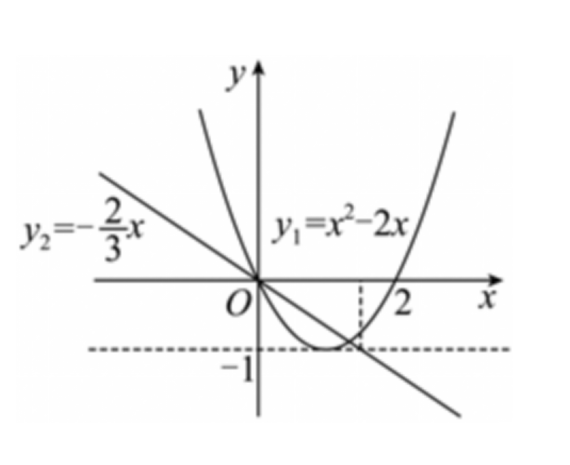
\includegraphics[width=0.24\textwidth]{figures/gao102_q7.png}
\end{center}
\step{当 $m>\dfrac32$ 时，当 $x>m$ 时 $f(x)\in\left(-\infty,-\dfrac23m\right)$，当 $x\leqslant m$ 时 $f(x)\in[-1,+\infty)$，}
\step{显然 $-\dfrac23m<-1$，此时函数 $f(x)$ 的值域不为 $R$，不符合题意；}
\step{当 $m<0$ 时，当 $x>m$ 时，$f(x)\in\left(-\infty,-\dfrac23m\right)$，}
\step{当 $x\leqslant m$ 时，$f(x)\in[m^2-2m,+\infty)$，}
\step{此时 $m^2-2m-\left(-\dfrac23m\right)=m^2-\dfrac43m=m\left(m-\dfrac43\right)>0$，即 $m^2-2m>-\dfrac23m$，}
\step{此时函数 $f(x)$ 的值域不为 $R$，不符合题意；}
\step{当 $0\leqslant m\leqslant\dfrac43$ 时，在 $x\in(0,m)$ 时 $y_2>y_1$，即 $m^2-2m<-\dfrac23m$，}
\step{此时 $f(x)$ 的值域为 $R$，符合题意，}
\step{当 $\dfrac43<m\leqslant\dfrac32$ 时，当 $x>m$ 时，$f(x)\in\left(-\infty,-\dfrac23m\right)$，}
\step{当 $x\leqslant m$ 时，$f(x)\in[-1,+\infty)$，}
\step{此时 $-1-\left(-\dfrac23m\right)=\dfrac23m-1\leqslant0$，即 $-1\leqslant-\dfrac23m$，}
\step{此时函数 $f(x)$ 的值域为 $R$，符合题意；}
\step{综上，$0\leqslant m\leqslant\dfrac32$，即实数 $m$ 的取值范围是 $\left[0,\dfrac32\right]$.}
\solend

\fi

\item 已知函数 $f(x)=x^2-2ax+b$（$a>1$）的定义域和值域都为 $[1,a]$，则 $b=$\blankline[4.4em].

\ifanswer
\solbegin
\step{$f(x)=x^2-2ax+b$（$a>1$）在 $[1,a]$ 严格减，}
\step{则 $f(1)=1-2a+b=a,f(a)=-a^2+b=1$，解得 $a=2,b=5$，所以 $b=5$.}
\solend

\fi

\item 若 $f(x)$ 满足 $f(x+y)=f(x)f(y)$，当 $x>0$ 时，$f(x)$ 的值域为 $(1,+\infty)$，则 $x<0$ 时，
$f(x)$ 的取值范围为\blankline[4.4em].

\ifanswer
\solbegin
\step{因为 $f(x+y)=f(x)f(y)$，令 $x=1$，$y=0$，得 $f(1+0)=f(1)f(0)$，}
\step{又因为当 $x>0$ 时，$f(x)>1$，所以 $f(1)>1>0$，故 $f(0)=1$.}
\step{当 $x<0$ 时，$-x>0$，令 $y=-x$，得 $f(x-x)=f(0)=1=f(x)f(-x)$，}
\step{故 $f(x)=\dfrac1{f(-x)}\in(0,1)$，故 $x<0$ 时，$f(x)$ 的取值范围为 $(0,1)$.}
\solend

\fi

\item 设函数 $f(x)=\begin{cases}x^2+x, & x<0\\ -x^2, & x\geqslant0\end{cases}$，若 $f(f(a))\leqslant2$，则实数 $a$ 的取值范围是\blankline[4.4em].

\ifanswer
\solbegin
\step{函数 $f(x)=\begin{cases}x^2+x, & x<0\\ -x^2, & x\geqslant0\end{cases}$，它的图象如图所示：}
\begin{center}
% 原图第 4 页解析插图直接裁取（原卷排于解析行右侧）。
% 裁框取图形区域，已去粉色水印转灰度。
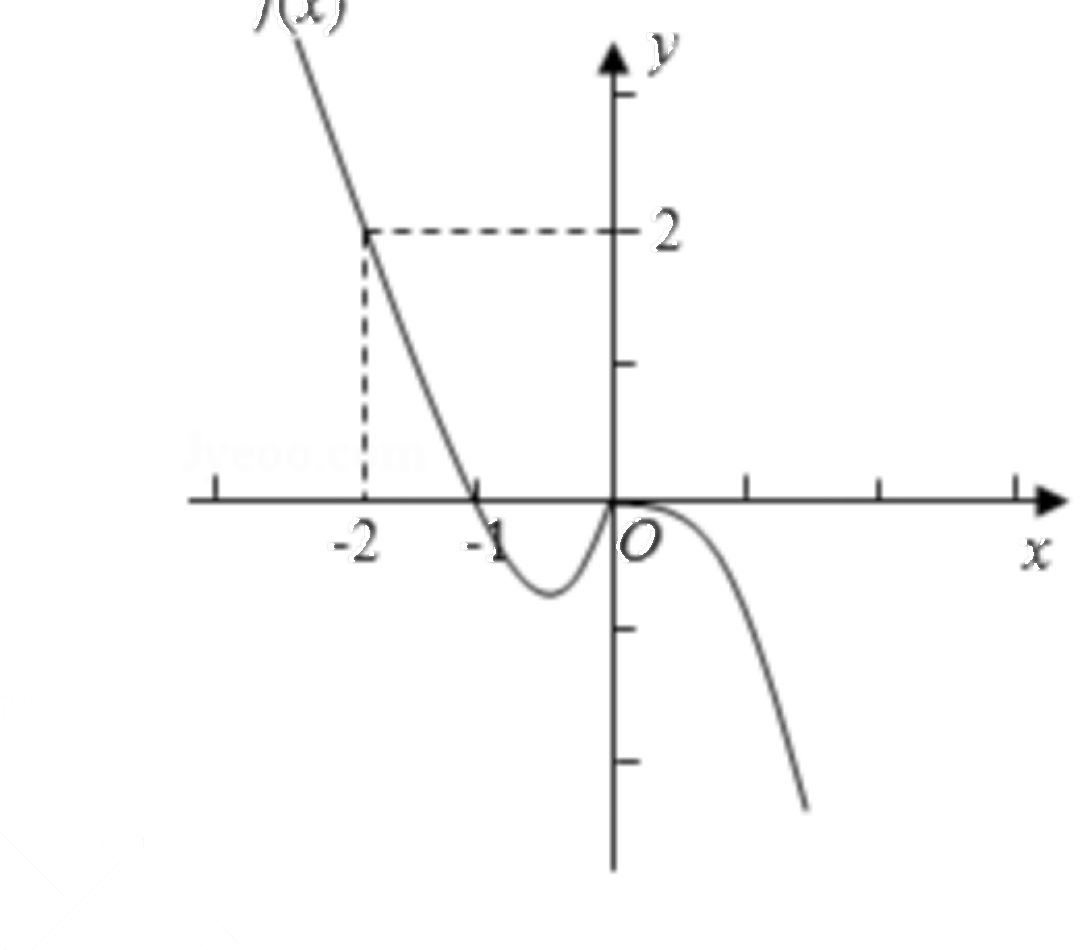
\includegraphics[width=0.30\textwidth]{figures/gao102_q10.png}
\end{center}
\step{由 $f(f(a))\leqslant2$，得 $f(a)\geqslant-2$.}
\step{当 $a<0$ 时，$f(a)=a^2+a=\left(a+\dfrac12\right)^2-\dfrac14\geqslant-2$ 恒成立；}
\step{当 $a\geqslant0$ 时，$f(a)=-a^2\geqslant-2$，即 $a^2\leqslant2$，解得 $0\leqslant a\leqslant\sqrt2$，}
\step{则实数 $a$ 的取值范围是 $(-\infty,\sqrt2]$.}
\solend

\fi

\item 已知二次函数 $f(x)$、$g(x)$ 的二次项系数均为 1，且满足
$\dfrac{f(2025)}{g(2025)}=\dfrac{f(2026)}{g(2026)}=\dfrac{2026}{2025}$，
则 $2026g(2027)-2025f(2027)$ 的值为\blankline[4.4em].

\ifanswer
\solbegin
\step{令 $h(x)=2026g(x)-2025f(x)$，其二次项系数为 $2026-2025=1$.}
\step{由比例条件得 $h(2025)=h(2026)=0$，}
\step{因此 $h(x)=(x-2025)(x-2026),h(2027)=2\times1=2$.}
\solend

\fi

\item 已知函数 $f(x)=\left\lvert x+\dfrac1x-a\right\rvert+1$，对任意实数 $x_1$、$x_2$、$x_3\in\left[\dfrac13,3\right]$，使得以
$f(x_1)$、$f(x_2)$、$f(x_3)$ 数值为边长可构成三角形，则实数 $a$ 的取值范围为\blankline[4.4em].

\ifanswer
\solbegin
\step{对任意实数 $x_1,x_2,x_3\in\left[\dfrac13,3\right]$，}
\step{使得以 $f(x_1)$、$f(x_2)$、$f(x_3)$ 数值为边长可构成三角形，}
\step{只需 $2f(x)_{\min}>f(x)_{\max}$，设 $g(x)=x+\dfrac1x-a$，}
\step{当 $x\in\left[\dfrac13,1\right)$ 时，函数 $g(x)$ 严格减，当 $x\in(1,3]$ 时，函数 $g(x)$ 严格增，}
\step{因为 $g(1)=2-a,g(3)=\dfrac{10}3-a,g\left(\dfrac13\right)=\dfrac{10}3-a$，所以 $g(x)\in\left[2-a,\dfrac{10}3-a\right]$，}
\step{当 $2-a\geqslant0$ 时，即 $a\leqslant2$ 时，$f(x)=\left\lvert x+\dfrac1x-a\right\rvert+1=g(x)+1$，}
\step{此时 $f(x)\in\left[3-a,\dfrac{13}3-a\right]$，}
\step{因此由 $2f(x)_{\min}>f(x)_{\max}\Rightarrow2(3-a)>\dfrac{13}3-a\Rightarrow a<\dfrac53$，而 $a\leqslant2$，所以 $a<\dfrac53$；}
\step{当 $\dfrac{10}3-a\leqslant0$，即 $a\geqslant\dfrac{10}3$ 时，$f(x)=\left\lvert x+\dfrac1x-a\right\rvert+1=-g(x)+1$，}
\step{此时 $f(x)\in\left[a-\dfrac73,a-1\right]$，}
\step{因此由 $2f(x)_{\min}>f(x)_{\max}\Rightarrow2\left(a-\dfrac73\right)>a-1\Rightarrow a>\dfrac{11}3$，而 $a\geqslant\dfrac{10}3$，所以 $a>\dfrac{11}3$，}
\step{若 $2-a<0<\dfrac{10}3-a$ 时，即 $2<a<\dfrac{10}3$ 时，}
\step{若 $a-2\geqslant\dfrac{10}3-a\Rightarrow a\geqslant\dfrac83$，即当 $\dfrac83\leqslant a<\dfrac{10}3$ 时，}
\step{显然此时 $f(x)_{\min}=1$，$f(x)_{\max}=a-2+1=a-1$，}
\step{由 $2f(x)_{\min}>f(x)_{\max}\Rightarrow2\times1>a-1\Rightarrow a<3$，显然 $\dfrac83\leqslant a<3$，}
\step{若 $a-2<\dfrac{10}3-a\Rightarrow a<\dfrac83$，即当 $2<a<\dfrac83$ 时，}
\step{显然此时 $f(x)_{\min}=1,f(x)_{\max}=\dfrac{10}3-a+1=\dfrac{13}3-a$，}
\step{因此由 $2f(x)_{\min}>f(x)_{\max}\Rightarrow2\times1>\dfrac{13}3-a\Rightarrow a>\dfrac73$，而 $\dfrac73<a<\dfrac83$，}
\step{综上，实数 $a$ 的取值范围为 $\left(-\infty,\dfrac53\right)\cup\left(\dfrac73,3\right)\cup\left(\dfrac{11}3,+\infty\right)$.}
\solend

\fi

\end{enumerate}

\bigsec{二、选择题}

\begin{enumerate}
\setcounter{enumi}{12}

\item 已知 $f(x)$ 是定义在 $\R$ 上的奇函数，$g(x)$ 是定义在 $\R$ 上的偶函数，则\mbox{（\quad）}

\keepwithprev
A. $f(x)g(x)$ 是偶函数\qquad B. $f(g(x))$ 是奇函数

C. $f(x)-g(x)$ 是奇函数\qquad D. $g(f(x))$ 是偶函数

\ifanswer
\solbegin
\step{$g(f(x))$ 的定义域为 $\R$，且 $g(f(-x))=g(-f(x))=g(f(x))$，}
\step{所以 $g(f(x))$ 是偶函数，故选 $D$.}
\solend

\fi

\item 已知定义在 $R$ 上的偶函数 $f(x)=\lvert x-m+1\rvert-2$，若正实数 $a$、$b$ 满足 $f(a)+f(2b)=m$，
则 $\dfrac1a+\dfrac2b$ 的最小值为\mbox{（\quad）}

\keepwithprev
A. $\dfrac95$\qquad\qquad B. $9$\qquad\qquad C. $\dfrac85$\qquad\qquad D. $8$

\ifanswer
\solbegin
\step{因为 $f(x)=\lvert x-m+1\rvert-2$ 是偶函数，所以 $-m+1=0$，所以 $m=1$，}
\step{所以 $f(x)=\lvert x\rvert-2$，若正实数 $a$、$b$ 满足 $f(a)+f(2b)=m$，}
\step{则 $a-2+2b-2=1$，所以 $a+2b=5$，}
\step{所以 $\dfrac1a+\dfrac2b=\dfrac15(a+2b)\left(\dfrac1a+\dfrac2b\right)=\dfrac15\left(5+\dfrac{2a}b+\dfrac{2b}a\right)\geqslant\dfrac95$，}
\step{当且仅当 $a=b=\dfrac53$ 时取等号，则 $\dfrac1a+\dfrac2b$ 的最小值为 $\dfrac95$，故选 $A$.}
\solend

\fi

\item 设函数 $g(x)=x^2-2$（$x\in\R$），$f(x)=\begin{cases}g(x)+x+4, & x<g(x)\\ g(x)-x, & x\geqslant g(x)\end{cases}$，则 $f(x)$ 的值域是

\mbox{（\quad）}

\keepwithprev
A. $\left[-\dfrac94,0\right]\cup(1,+\infty)$\qquad\qquad B. $[0,+\infty)$

C. $\left[-\dfrac94,+\infty\right)$\qquad\qquad D. $\left[-\dfrac94,0\right]\cup(2,+\infty)$

\ifanswer
\solbegin
\step{当 $x<g(x)$，即 $x<x^2-2$，$(x-2)(x+1)>0$ 时，$x>2$ 或 $x<-1$，}
\step{$f(x)=g(x)+x+4=x^2-2+x+4=x^2+x+2=(x+0.5)^2+1.75$，}
\step{其最小值趋向于 $f(-1)$ 即 2，无最大值，}
\step{因此这个区间的值域为 $(2,+\infty)$.}
\step{当 $x\geqslant g(x)$ 时，$-1\leqslant x\leqslant2$，$f(x)=g(x)-x=x^2-2-x=(x-0.5)^2-2.25$，}
\step{其最小值为 $f(0.5)=-2.25$，其最大值为 $f(2)=0$，}
\step{因此这区间的值域为 $[-2.25,0]$.}
\step{综上，函数值域为 $\left[-\dfrac94,0\right]\cup(2,+\infty)$，故选 $D$.}
\solend

\fi

\item 设 $D$ 是含数 1 的有限实数集，$f(x)$ 是定义在 $D$ 上的函数，若 $f(x)$ 的图象绕原点逆时针
旋转 $\dfrac{\pi}{6}$ 与原图象重合，则在以下各项中，$f(1)$ 的可能取值只能是\mbox{（\quad）}

\keepwithprev
A. $\sqrt3$\qquad\qquad B. $\dfrac{\sqrt3}2$\qquad\qquad C. $\dfrac{\sqrt3}3$\qquad\qquad D. $0$

\ifanswer
\solbegin
\step{问题相当于圆上由 12 个点为一组，每次绕原点逆时针旋转 $\dfrac{\pi}{6}$ 个单位后与下一个点}
\step{会重合。我们可以通过代入和赋值的方法，当 $f(1)=\sqrt3$、$\dfrac{\sqrt3}3$、$0$ 时，}
\step{此时得到的圆心角为 $\dfrac{\pi}{3}$、$\dfrac{\pi}{6}$、$0$，然而此时 $x=0$ 或者 $x=1$ 时，}
\step{都有 2 个 $y$ 与之对应，而我们知道函数的定义就是要求一个 $x$ 只能对应一个 $y$，}
\step{因此只有当 $x=\dfrac{\sqrt3}2$，此时旋转 $\dfrac{\pi}{6}$，此时满足一个 $x$ 只会对应一个 $y$，故选 $B$.}
\solend

\fi

\end{enumerate}

\bigsec{三、解答题}

\begin{enumerate}
\setcounter{enumi}{16}

\item 求下列函数的值域.

（1）$y=\dfrac{2x^2-3x+5}{x-1}\left(x\in\left[\dfrac32,3\right]\right)$；

（2）$f(x)=\sqrt{x}-\sqrt{2-x}+\sqrt{x(2-x)}$.

\ansspace*[10]

\ifanswer
\solbegin
\stepm{（1）}{令 $t=x-1$，则 $t\in\left[\dfrac12,2\right]$，原函数化为 $Y(t)=2t+\dfrac4t+1$.}
\step{当 $0<u<v$ 时，$Y(v)-Y(u)=2(v-u)\left(1-\dfrac2{uv}\right)$，}
\step{所以 $Y$ 在 $\left[\dfrac12,\sqrt2\right]$ 上严格递减，在 $[\sqrt2,2]$ 上严格递增.}
\step{由 $Y(\sqrt2)=4\sqrt2+1,Y\left(\dfrac12\right)=10,Y(2)=7$，得值域为 $[4\sqrt2+1,10]$.}
\stepm{（2）}{定义域为 $[0,2]$.}
\step{令 $s=\sqrt{x}-\sqrt{2-x}$，$\sqrt{x}$ 与 $-\sqrt{2-x}$ 均随 $x$ 严格递增，}
\step{$s$ 从 $-\sqrt2$ 递增到 $\sqrt2$，即 $s\in[-\sqrt2,\sqrt2]$.}
\step{由 $s^2=2-2\sqrt{x(2-x)}$，得 $f(x)=s+\dfrac{2-s^2}2=-\dfrac12(s-1)^2+\dfrac32$.}
\step{当 $s=1$ 时取得最大值 $\dfrac32$；当 $s=-\sqrt2$ 时取得最小值 $-\sqrt2$；}
\step{因此值域为 $\left[-\sqrt2,\dfrac32\right]$.}
\solend

\fi

\item 已知 $f(2x+1)=\dfrac{2x+1}{x+1}$.

（1）解不等式 $f(x)<x$；

（2）求 $f(1)+f(2)+\cdots+f(6)+f\left(\dfrac12\right)+f\left(\dfrac13\right)+\cdots+f\left(\dfrac16\right)$ 的值.

\ansspace*[12]

\ifanswer
\solbegin
\step{令 $t=2x+1$，则 $x=\dfrac{t-1}2$，得 $f(t)=\dfrac{2t}{t+1},t\neq-1$.}
\stepm{（1）}{不等式等价于 $\dfrac{2x}{x+1}<x\Leftrightarrow\dfrac{x(x-1)}{x+1}>0$.}
\step{以 $-1,0,1$ 分区间判断符号，得解集为 $(-1,0)\cup(1,+\infty)$.}
\stepm{（2）}{当 $x>0$ 时，$f(x)+f\left(\dfrac1x\right)=\dfrac{2x}{x+1}+\dfrac2{x+1}=2$.}
\step{将 $f(2),\cdots,f(6)$ 分别与其倒数对应的函数值配对，共 5 对，且 $f(1)=1$，}
\step{因此原式$=1+5\times2=11$.}
\solend

\fi

\item 已知函数 $f(x)$、$g(x)$ 是定义在 $R$ 上的函数，其中 $f(x)$ 是奇函数，$g(x)$ 是偶函数，且
$f(x)+g(x)=ax^2-x$.

（1）求 $f(x)$ 和 $g(x)$ 的解析式；

（2）$h(x)=f(x)+g(x)+(1-a)x^2-2ax+4$ 在 $[1,3]$ 上有两个零点，求实数 $a$ 的取值范
围.

\ansspace*[14]

\ifanswer
\solbegin
\stepm{（1）}{因为 $f(x)+g(x)=ax^2-x$①，所以 $f(-x)+g(-x)=ax^2+x$，}
\step{又 $f(x)$ 是奇函数，$g(x)$ 是偶函数，}
\step{所以 $f(-x)=-f(x)$，$g(-x)=g(x)$，}
\step{所以 $-f(x)+g(x)=ax^2+x$②，}
\step{联立①②解得 $f(x)=-x$，$g(x)=ax^2$.}
\stepm{（2）}{$h(x)=f(x)+g(x)+(1-a)x^2-2ax+4$}
\step{$=ax^2-x+(1-a)x^2-2ax+4=x^2-(2a+1)x+4$，}
\step{是开口向上，对称轴为 $x=\dfrac{2a+1}2$ 的二次函数，}
\step{因为 $h(x)$ 在 $[1,3]$ 上有两个零点，所以 $\begin{cases}\Delta=(2a+1)^2-16>0\\ 1<\dfrac{2a+1}2<3\\ h(1)=1-(2a+1)+4\geqslant0\\ h(3)=9-3(2a+1)+4\geqslant0\end{cases}$，}
\step{解得 $\dfrac32<a\leqslant\dfrac53$，故实数 $a$ 的取值范围为 $\left(\dfrac32,\dfrac53\right]$.}
\solend

\fi

\item 若函数 $f(x)$ 在区间 $[a,b]$ 上的值域恰为 $\left[\dfrac1b,\dfrac1a\right]$，则称区间 $[a,b]$ 为 $f(x)$ 的一个“倒域
区间”。已知定义在 $[-4,4]$ 上的奇函数 $g(x)$，当 $x\in[0,4]$ 时，$g(x)=-x^2+2x$.

（1）求 $g(x)$ 的解析式；

（2）若关于 $x$ 的方程 $g(x)=-mx-m$ 在 $(0,4)$ 上恰有两个不相等的实数根，求实数 $m$ 的
取值范围；

（3）求函数 $g(x)$ 在 $[-4,0]$ 内的“倒域区间”.

\ansspace*[16]

\ifanswer
\solbegin
\stepm{（1）}{当 $x\in[-4,0)$ 时，$-x\in(0,4]$，}
\step{由奇函数的定义得 $g(x)=-g(-x)=-[(-x)^2+2(-x)]=x^2+2x$，}
\step{所以 $g(x)=\begin{cases}-x^2+2x, & 0\leqslant x\leqslant4\\ x^2+2x, & -4\leqslant x<0\end{cases}$.}
\stepm{（2）}{方程 $g(x)=-mx-m$，即 $x^2-(m+2)x-m=0$，}
\step{设 $h(x)=x^2-(m+2)x-m$，$0<x<4$，}
\step{由题意得 $\begin{cases}h(0)=-m>0\\ h(4)=8-5m>0\\ \Delta=(m+2)^2+4m>0\\ 0<\dfrac{m+2}2<4\end{cases}$，解得 $2\sqrt3-4<m<0$，}
\step{即实数 $m$ 的取值范围是 $(2\sqrt3-4,0)$.}
\stepm{（3）}{易得当 $-4\leqslant a<b<0$ 时，$\dfrac1b<\dfrac1a$，}
\step{且 $g(x)$ 在 $[-4,-1]$ 上严格减，在 $[-1,0]$ 上严格增，}
\step{故当 $x\in[-4,0]$ 时，$g(x)_{\min}=g(-1)=-1$，}
\step{所以 $\dfrac1b\geqslant-1$，所以 $-4<b\leqslant-1$，所以 $-4\leqslant a<b\leqslant-1$，}
\step{则 $\begin{cases}g(a)=a^2+2a=\dfrac1a\\ g(b)=b^2+2b=\dfrac1b\\ -4\leqslant a<b\leqslant-1\end{cases}$，解得 $\begin{cases}a=-\dfrac{1+\sqrt5}2\\ b=-1\end{cases}$，}
\step{所以 $g(x)$ 在 $[-4,0]$ 内的“倒域区间”为 $\left[-\dfrac{1+\sqrt5}2,-1\right]$.}
\solend

\fi

\item 我们知道：函数 $y=f(x)$ 的图象关于坐标原点成中心对称图形的充要条件是函数
$y=f(x)$ 为奇函数。有同学发现可以推广为：函数 $y=f(x)$ 的图象关于点 $(a,b)$ 成中心对
称图形的充要条件为函数 $y=f(x+a)-b$ 为奇函数。已知函数 $f(x)=\dfrac{2x}{3-x}$.

（1）求函数 $f(x)$ 图象的对称中心；

（2）若定义在 $R$ 上的函数 $y=g(x)$ 的图象关于点 $(1,2)$ 对称，且 $g(1)=2$，当 $x\in[0,1)$
时，$g(x)=x^2-tx+t+1$.

（$i$）求 $g(-3)+g(5)$ 的值；

（$ii$）若对$\forall x_1\in[0,2]$，$\exists x_2\in[-3,2]$ 使得 $g(x_1)=f(x_2)$ 恒成立，求实数 $t$ 的取值范围.

\ansspace*[18]

\ifanswer
\solbegin
\stepm{（1）}{由 $f(x)=\dfrac{2x}{3-x}=-2+\dfrac6{3-x}$，}
\step{易得 $f(x+3)+2=-2+\dfrac6{3-(x+3)}+2=-\dfrac6x$ 为奇函数，}
\step{$f(x)$ 的图象关于 $(3,-2)$ 对称.}
\stepm{（2）}{（$i$）$y=g(x)$ 图象关于点 $(1,2)$ 对称，则 $g(1+x)+g(1-x)=4$，}
\step{令 $x=4$，则 $g(-3)+g(5)=4$.}
\step{（$ii$）有 $g(x)$ 在 $x\in[0,2]$ 的取值范围为 $f(x)$ 在 $x\in[-3,2]$ 的取值范围的}
\step{子集，}
\step{因为 $f(x)=\dfrac{2x}{3-x}=\dfrac{6-2(3-x)}{3-x}=\dfrac6{3-x}-2$ 在 $[-3,2]$ 上严格增，}
\step{所以 $f(x)$ 在 $x\in[-3,2]$ 上的取值范围为 $[-1,4]$，}
\step{记 $g(x)$ 的值域为 $A$，且 $g(1)=2$，当 $x\in[0,1)$ 时 $g(x)=x^2-tx+t+1$，}
\step{①当 $\dfrac t2\leqslant0$，即 $t\leqslant0$ 时，有 $g(x)$ 在 $[0,1)$ 上严格增，}
\step{由对称性得 $g(x)$ 在 $[1,2]$ 上严格增，故 $g(x)$ 在 $[0,2]$ 上严格增，}
\step{故 $g(x)_{\min}=g(0)=t+1$，$g(x)_{\max}=g(2)=4-(t+1)=3-t$，$t\leqslant0$，}
\step{则 $A=[t+1,3-t]\subseteq[-1,4]$，即 $\begin{cases}t\leqslant0\\ t+1\geqslant-1\\ 3-t\leqslant4\end{cases}$，解得 $-1\leqslant t\leqslant0$.}
\step{②当 $0<\dfrac t2<1$，即 $0<t<2$ 时，}
\step{$g(x)$ 在 $\left(0,\dfrac t2\right)$ 上严格减，在 $\left(\dfrac t2,1\right)$ 上严格增，}
\step{由对称性得 $g(x)$ 在 $\left(2-\dfrac t2,2\right)$ 上严格减，在 $\left(1,2-\dfrac t2\right)$ 上严格增，}
\step{故 $g(x)$ 在 $\left(0,\dfrac t2\right)$ 上严格减，在 $\left(\dfrac t2,2-\dfrac t2\right)$ 上严格增，}
\step{在 $\left(2-\dfrac t2,2\right)$ 上严格减，则 $A=\left[g\left(\dfrac t2\right),g\left(2-\dfrac t2\right)\right]$，}
\step{由 $0<t<2$，得 $g(0)=t+1\in(1,3)$，$g(2)=4-(t+1)=3-t\in(1,3)$，}
\step{$g\left(\dfrac t2\right)=-\dfrac{t^2}4+t+1=-\dfrac14(t-2)^2+2\in(1,2]$，}
\step{又 $g\left(\dfrac t2\right)+g\left(2-\dfrac t2\right)=4$，$g\left(2-\dfrac t2\right)\in(2,3)$，}
\step{当 $0<t<2$ 时，$A\subseteq[-1,4]$ 恒成立，}
\step{③当 $\dfrac t2\geqslant1$，即 $t\geqslant2$ 时，有 $g(x)$ 在 $[0,1)$ 上严格减，}
\step{由对称点 $(1,2)$ 得 $g(x)$ 在 $[1,2]$ 上严格减，所以 $g(x)$ 在 $[0,2]$ 上严格减，}
\step{故 $g(x)_{\max}=g(0)=t+1$，$g(x)_{\min}=g(2)=4-(t+1)=3-t$，$t\geqslant2$，}
\step{则 $A=[3-t,t+1]\subseteq[-1,4]$，即 $\begin{cases}t\geqslant2\\ t+1\leqslant4\\ 3-t\geqslant-1\end{cases}$，解得 $2\leqslant t\leqslant3$.}
\step{综上，$t$ 的范围为 $\{t\mid-1\leqslant t\leqslant3\}$.}
\solend

\fi

\end{enumerate}

\end{document}
"
%
% 原始材料：微信公众号“魔都数学加油站”文章，作者破晓，2026-11-01 21:56 发布；
% 连载“27学年高一102”，原文标题“27学年高一102——2026-2027年上海市华师大二附中高一上周末作业5函数”；
% 原文链接：https://mp.weixin.qq.com/s/CDvOCcxFskIe9aFUeKi3Ww。
% 正文为 13 张 PNG 页（第 1、2、10、13 页 2560×3620，其余 4762×6735），题目下印有【解析】，为讲评版。
% 题目、解析均据原图转录；卷面水印及公众号页脚未录入。
%
% 卷首标题：原卷印作“2026-2027 年华师大二附中高一上周末作业 5”（公众号标题中的“上海市”“函数”
% 卷面标题行没有，本稿照卷面），年份区间按全稿惯例排 en dash；原卷未印副标题，本稿按题目内容
% 标为“函数”（全稿首份以函数为单一模块的卷子）。
%
% 与原卷的排版差异：
%   ① 原文从第 3 题起，填空题编号为 3—12、选择题为 13—16、解答题为 17—21，本稿保留原题号；
%   ② 原卷每题下直接印【解析】，本稿按全稿惯例将解析置于答案版；选择题括号内未印答案，另由
%      解析末句“故选 X”给出；
%   ③ 原卷未印副标题，本稿按“知识模块”口径补出；
%   ④ 原卷填空横线按全稿惯例排为 \blankline[4.4em]；解答题按惯例加 \ansspace；选择题括号排
%      \mbox{（\quad）}、选项段前按惯例加 \keepwithprev；
%   ⑤ 原卷 $f(x)_{min}$、$f(x)_{max}$ 等下标排斜体，按 高一96 成例改正体 $\min$、$\max$；
%   ⑥ 原卷数集排斜体 $R$（第 13 题排粗体），按全稿惯例改 $\R$；
%   ⑦ 第 7、10 两题的解析插图裁自原图（去粉色水印转灰度），仅答案版显示。
%
% 原卷存疑／笔误（均照录加注）：
%   第 3 题解析“减去都对应 −2 和 2 的”措辞含糊（意为减去恒取 −2 与恒取 2 的两个常函数）；
%   第 15 题解析“其最小值趋向于 f(−1) 即 2”（该段 f(x)=x²+x+2 在 x→−1⁻ 时趋于 2、取不到）；
%   第 16 题解析末句“因此只有当 x=√3/2”（按上下文应为 f(1)=√3/2）；
%   第 16 题解析以 f(1)=√3、√3/3、0 赋值时称“得到的圆心角为 π/3、π/6、0”，其中 √3/3 对应
%   圆心角 π/6 的说法与该点 (1,√3/3) 的实际幅角一致，但与选项 C（√3/3）被排除的结论矛盾
%   （幅角 π/6 的点旋转 π/6 后落到幅角 π/3 处，仍占 12 等分点位，原卷解析未展开），照录。
%
% 行数核对：逐题数 \step/\stepm 条数，合计 155 条（Q3：2；Q4：3；Q5：6；Q6：5；Q7：19；
% Q8：2；Q9：4；Q10：5；Q11：3；Q12：19；Q13：2；Q14：5；Q15：8；Q16：5；Q17：10；
% Q18：6；Q19：10；Q20：13；Q21：28），与原卷印刷行逐题相等。
%
\documentclass[a4paper,11pt]{article}
\usepackage{common}

\begin{document}

\examtitlest[3]{2026--2027 年华师大二附中高一上周末作业 5}{函数}

\bigsec{一、填空题}

\begin{enumerate}
\setcounter{enumi}{2}

\item 已知函数 $y=f(x)$ 的定义域为 $\{-2,-1,1,2\}$，值域为 $\{-2,2\}$，则满足条件的函数
$y=f(x)$ 最多有\blankline[4.4em]个.

\ifanswer
\solbegin
\step{定义域中 4 个元素每个都可以对应 $-2$ 和 $2$ 中的一个，减去都对应 $-2$ 和 $2$ 的，}
\step{则满足条件的函数 $y=f(x)$ 最多有 $2^4-2=14$.}
\solend

\fi

\item 已知函数 $f(2x)$ 的定义域为 $[-2,2]$，则函数 $f(x-3)$ 的定义域为\blankline[4.4em].

\ifanswer
\solbegin
\step{因为函数 $f(2x)$ 的定义域为 $[-2,2]$，即 $-2\leqslant x\leqslant2$，所以 $-4\leqslant2x\leqslant4$，}
\step{得 $f(x)$ 的定义域为 $[-4,4]$，由 $-4\leqslant x-3\leqslant4$，解得 $-1\leqslant x\leqslant7$，}
\step{即函数 $f(x-3)$ 的定义域为 $[-1,7]$.}
\solend

\fi

\item 函数 $f(x)=\begin{cases}-x-1, & x<0\\ -x+1, & x>0\end{cases}$，则 $f(x)-f(-x)>1$ 的解集为\blankline[4.4em].

\ifanswer
\solbegin
\step{定义域为 $\{x\mid x\neq0\}$.}
\step{当 $x<0$ 时，$-x>0,f(-x)=x+1$，}
\step{$f(x)-f(-x)=(-x-1)-(x+1)=-2x-2>1$，得 $x<-\dfrac32$.}
\step{当 $x>0$ 时，$f(-x)=x-1,f(x)-f(-x)=(-x+1)-(x-1)=-2x+2>1$，}
\step{得 $0<x<\dfrac12$.}
\step{故解集为 $\left(-\infty,-\dfrac32\right)\cup\left(0,\dfrac12\right)$.}
\solend

\fi

\item 已知函数 $f(x)=x^2-2(m-3)x+5$ 在区间 $[2,+\infty)$ 上的最小值为 1，则实数 $m=$\blankline[4.4em].

\ifanswer
\solbegin
\step{函数 $f(x)$ 图象的对称轴为 $x=m-3$.}
\step{当 $m-3\leqslant2$，即 $m\leqslant5$ 时，$f(x)_{\min}=f(2)=9-4m+12=1$，解得 $m=5$；}
\step{当 $m-3>2$，即 $m>5$ 时，$f(x)_{\min}=f(m-3)=-m^2+6m-4=1$，}
\step{解得 $m=5$（舍去）或 $1$（舍去），}
\step{综上，$m=5$.}
\solend

\fi

\item 已知函数 $f(x)=\begin{cases}x^2-2x, & x\leqslant m\\ -\dfrac23x, & x>m\end{cases}$ 的值域为 $R$，则实数 $m$ 的取值范围是\blankline[4.4em].

\ifanswer
\solbegin
\step{对于函数 $y_1=x^2-2x$，则 $y_1=(x-1)^2-1\geqslant-1$，当且仅当 $x=1$ 时取等号，}
\step{且函数在 $(-\infty,1)$ 上严格减，在 $(1,+\infty)$ 上严格增，}
\step{对于函数 $y_2=-\dfrac23x$，令 $y_2=-1$，则 $x=\dfrac32$，且函数在定义域上严格减，}
\step{令 $x^2-2x=-\dfrac23x$，解得 $x=0$ 或 $x=\dfrac43$，}
\step{所以 $y_2=-\dfrac23x$ 与 $y_1=x^2-2x$ 的两个交点分别为 $(0,0)$、$\left(\dfrac43,-\dfrac89\right)$，}
\step{则函数 $y_2=-\dfrac23x$ 与 $y_1=x^2-2x$ 的图象如图所示：}
\begin{center}
% 原图第 2 页解析插图直接裁取（原卷排于解析行右侧）。
% 裁框取图形区域，已去粉色水印转灰度。
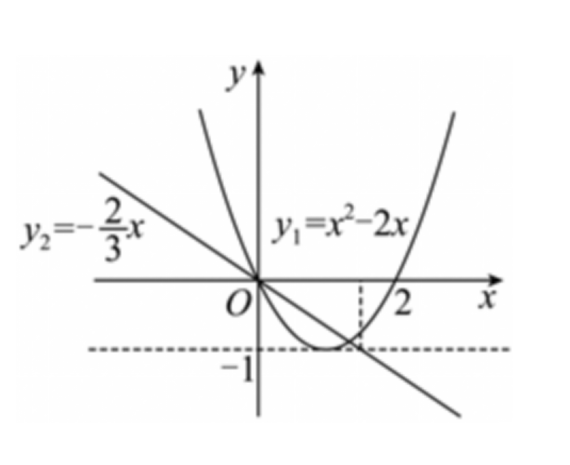
\includegraphics[width=0.24\textwidth]{figures/gao102_q7.png}
\end{center}
\step{当 $m>\dfrac32$ 时，当 $x>m$ 时 $f(x)\in\left(-\infty,-\dfrac23m\right)$，当 $x\leqslant m$ 时 $f(x)\in[-1,+\infty)$，}
\step{显然 $-\dfrac23m<-1$，此时函数 $f(x)$ 的值域不为 $R$，不符合题意；}
\step{当 $m<0$ 时，当 $x>m$ 时，$f(x)\in\left(-\infty,-\dfrac23m\right)$，}
\step{当 $x\leqslant m$ 时，$f(x)\in[m^2-2m,+\infty)$，}
\step{此时 $m^2-2m-\left(-\dfrac23m\right)=m^2-\dfrac43m=m\left(m-\dfrac43\right)>0$，即 $m^2-2m>-\dfrac23m$，}
\step{此时函数 $f(x)$ 的值域不为 $R$，不符合题意；}
\step{当 $0\leqslant m\leqslant\dfrac43$ 时，在 $x\in(0,m)$ 时 $y_2>y_1$，即 $m^2-2m<-\dfrac23m$，}
\step{此时 $f(x)$ 的值域为 $R$，符合题意，}
\step{当 $\dfrac43<m\leqslant\dfrac32$ 时，当 $x>m$ 时，$f(x)\in\left(-\infty,-\dfrac23m\right)$，}
\step{当 $x\leqslant m$ 时，$f(x)\in[-1,+\infty)$，}
\step{此时 $-1-\left(-\dfrac23m\right)=\dfrac23m-1\leqslant0$，即 $-1\leqslant-\dfrac23m$，}
\step{此时函数 $f(x)$ 的值域为 $R$，符合题意；}
\step{综上，$0\leqslant m\leqslant\dfrac32$，即实数 $m$ 的取值范围是 $\left[0,\dfrac32\right]$.}
\solend

\fi

\item 已知函数 $f(x)=x^2-2ax+b$（$a>1$）的定义域和值域都为 $[1,a]$，则 $b=$\blankline[4.4em].

\ifanswer
\solbegin
\step{$f(x)=x^2-2ax+b$（$a>1$）在 $[1,a]$ 严格减，}
\step{则 $f(1)=1-2a+b=a,f(a)=-a^2+b=1$，解得 $a=2,b=5$，所以 $b=5$.}
\solend

\fi

\item 若 $f(x)$ 满足 $f(x+y)=f(x)f(y)$，当 $x>0$ 时，$f(x)$ 的值域为 $(1,+\infty)$，则 $x<0$ 时，
$f(x)$ 的取值范围为\blankline[4.4em].

\ifanswer
\solbegin
\step{因为 $f(x+y)=f(x)f(y)$，令 $x=1$，$y=0$，得 $f(1+0)=f(1)f(0)$，}
\step{又因为当 $x>0$ 时，$f(x)>1$，所以 $f(1)>1>0$，故 $f(0)=1$.}
\step{当 $x<0$ 时，$-x>0$，令 $y=-x$，得 $f(x-x)=f(0)=1=f(x)f(-x)$，}
\step{故 $f(x)=\dfrac1{f(-x)}\in(0,1)$，故 $x<0$ 时，$f(x)$ 的取值范围为 $(0,1)$.}
\solend

\fi

\item 设函数 $f(x)=\begin{cases}x^2+x, & x<0\\ -x^2, & x\geqslant0\end{cases}$，若 $f(f(a))\leqslant2$，则实数 $a$ 的取值范围是\blankline[4.4em].

\ifanswer
\solbegin
\step{函数 $f(x)=\begin{cases}x^2+x, & x<0\\ -x^2, & x\geqslant0\end{cases}$，它的图象如图所示：}
\begin{center}
% 原图第 4 页解析插图直接裁取（原卷排于解析行右侧）。
% 裁框取图形区域，已去粉色水印转灰度。
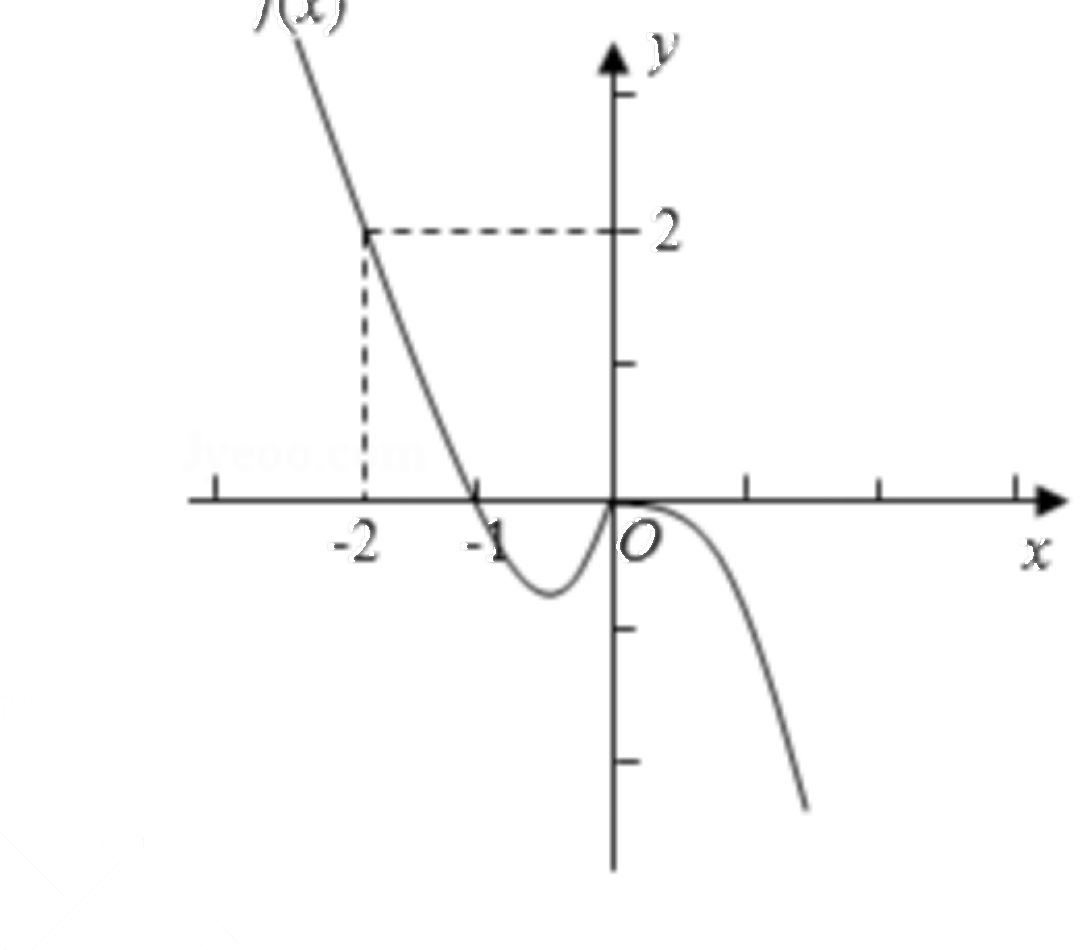
\includegraphics[width=0.30\textwidth]{figures/gao102_q10.png}
\end{center}
\step{由 $f(f(a))\leqslant2$，得 $f(a)\geqslant-2$.}
\step{当 $a<0$ 时，$f(a)=a^2+a=\left(a+\dfrac12\right)^2-\dfrac14\geqslant-2$ 恒成立；}
\step{当 $a\geqslant0$ 时，$f(a)=-a^2\geqslant-2$，即 $a^2\leqslant2$，解得 $0\leqslant a\leqslant\sqrt2$，}
\step{则实数 $a$ 的取值范围是 $(-\infty,\sqrt2]$.}
\solend

\fi

\item 已知二次函数 $f(x)$、$g(x)$ 的二次项系数均为 1，且满足
$\dfrac{f(2025)}{g(2025)}=\dfrac{f(2026)}{g(2026)}=\dfrac{2026}{2025}$，
则 $2026g(2027)-2025f(2027)$ 的值为\blankline[4.4em].

\ifanswer
\solbegin
\step{令 $h(x)=2026g(x)-2025f(x)$，其二次项系数为 $2026-2025=1$.}
\step{由比例条件得 $h(2025)=h(2026)=0$，}
\step{因此 $h(x)=(x-2025)(x-2026),h(2027)=2\times1=2$.}
\solend

\fi

\item 已知函数 $f(x)=\left\lvert x+\dfrac1x-a\right\rvert+1$，对任意实数 $x_1$、$x_2$、$x_3\in\left[\dfrac13,3\right]$，使得以
$f(x_1)$、$f(x_2)$、$f(x_3)$ 数值为边长可构成三角形，则实数 $a$ 的取值范围为\blankline[4.4em].

\ifanswer
\solbegin
\step{对任意实数 $x_1,x_2,x_3\in\left[\dfrac13,3\right]$，}
\step{使得以 $f(x_1)$、$f(x_2)$、$f(x_3)$ 数值为边长可构成三角形，}
\step{只需 $2f(x)_{\min}>f(x)_{\max}$，设 $g(x)=x+\dfrac1x-a$，}
\step{当 $x\in\left[\dfrac13,1\right)$ 时，函数 $g(x)$ 严格减，当 $x\in(1,3]$ 时，函数 $g(x)$ 严格增，}
\step{因为 $g(1)=2-a,g(3)=\dfrac{10}3-a,g\left(\dfrac13\right)=\dfrac{10}3-a$，所以 $g(x)\in\left[2-a,\dfrac{10}3-a\right]$，}
\step{当 $2-a\geqslant0$ 时，即 $a\leqslant2$ 时，$f(x)=\left\lvert x+\dfrac1x-a\right\rvert+1=g(x)+1$，}
\step{此时 $f(x)\in\left[3-a,\dfrac{13}3-a\right]$，}
\step{因此由 $2f(x)_{\min}>f(x)_{\max}\Rightarrow2(3-a)>\dfrac{13}3-a\Rightarrow a<\dfrac53$，而 $a\leqslant2$，所以 $a<\dfrac53$；}
\step{当 $\dfrac{10}3-a\leqslant0$，即 $a\geqslant\dfrac{10}3$ 时，$f(x)=\left\lvert x+\dfrac1x-a\right\rvert+1=-g(x)+1$，}
\step{此时 $f(x)\in\left[a-\dfrac73,a-1\right]$，}
\step{因此由 $2f(x)_{\min}>f(x)_{\max}\Rightarrow2\left(a-\dfrac73\right)>a-1\Rightarrow a>\dfrac{11}3$，而 $a\geqslant\dfrac{10}3$，所以 $a>\dfrac{11}3$，}
\step{若 $2-a<0<\dfrac{10}3-a$ 时，即 $2<a<\dfrac{10}3$ 时，}
\step{若 $a-2\geqslant\dfrac{10}3-a\Rightarrow a\geqslant\dfrac83$，即当 $\dfrac83\leqslant a<\dfrac{10}3$ 时，}
\step{显然此时 $f(x)_{\min}=1$，$f(x)_{\max}=a-2+1=a-1$，}
\step{由 $2f(x)_{\min}>f(x)_{\max}\Rightarrow2\times1>a-1\Rightarrow a<3$，显然 $\dfrac83\leqslant a<3$，}
\step{若 $a-2<\dfrac{10}3-a\Rightarrow a<\dfrac83$，即当 $2<a<\dfrac83$ 时，}
\step{显然此时 $f(x)_{\min}=1,f(x)_{\max}=\dfrac{10}3-a+1=\dfrac{13}3-a$，}
\step{因此由 $2f(x)_{\min}>f(x)_{\max}\Rightarrow2\times1>\dfrac{13}3-a\Rightarrow a>\dfrac73$，而 $\dfrac73<a<\dfrac83$，}
\step{综上，实数 $a$ 的取值范围为 $\left(-\infty,\dfrac53\right)\cup\left(\dfrac73,3\right)\cup\left(\dfrac{11}3,+\infty\right)$.}
\solend

\fi

\end{enumerate}

\bigsec{二、选择题}

\begin{enumerate}
\setcounter{enumi}{12}

\item 已知 $f(x)$ 是定义在 $\R$ 上的奇函数，$g(x)$ 是定义在 $\R$ 上的偶函数，则\mbox{（\quad）}

\keepwithprev
A. $f(x)g(x)$ 是偶函数\qquad B. $f(g(x))$ 是奇函数

C. $f(x)-g(x)$ 是奇函数\qquad D. $g(f(x))$ 是偶函数

\ifanswer
\solbegin
\step{$g(f(x))$ 的定义域为 $\R$，且 $g(f(-x))=g(-f(x))=g(f(x))$，}
\step{所以 $g(f(x))$ 是偶函数，故选 $D$.}
\solend

\fi

\item 已知定义在 $R$ 上的偶函数 $f(x)=\lvert x-m+1\rvert-2$，若正实数 $a$、$b$ 满足 $f(a)+f(2b)=m$，
则 $\dfrac1a+\dfrac2b$ 的最小值为\mbox{（\quad）}

\keepwithprev
A. $\dfrac95$\qquad\qquad B. $9$\qquad\qquad C. $\dfrac85$\qquad\qquad D. $8$

\ifanswer
\solbegin
\step{因为 $f(x)=\lvert x-m+1\rvert-2$ 是偶函数，所以 $-m+1=0$，所以 $m=1$，}
\step{所以 $f(x)=\lvert x\rvert-2$，若正实数 $a$、$b$ 满足 $f(a)+f(2b)=m$，}
\step{则 $a-2+2b-2=1$，所以 $a+2b=5$，}
\step{所以 $\dfrac1a+\dfrac2b=\dfrac15(a+2b)\left(\dfrac1a+\dfrac2b\right)=\dfrac15\left(5+\dfrac{2a}b+\dfrac{2b}a\right)\geqslant\dfrac95$，}
\step{当且仅当 $a=b=\dfrac53$ 时取等号，则 $\dfrac1a+\dfrac2b$ 的最小值为 $\dfrac95$，故选 $A$.}
\solend

\fi

\item 设函数 $g(x)=x^2-2$（$x\in\R$），$f(x)=\begin{cases}g(x)+x+4, & x<g(x)\\ g(x)-x, & x\geqslant g(x)\end{cases}$，则 $f(x)$ 的值域是

\mbox{（\quad）}

\keepwithprev
A. $\left[-\dfrac94,0\right]\cup(1,+\infty)$\qquad\qquad B. $[0,+\infty)$

C. $\left[-\dfrac94,+\infty\right)$\qquad\qquad D. $\left[-\dfrac94,0\right]\cup(2,+\infty)$

\ifanswer
\solbegin
\step{当 $x<g(x)$，即 $x<x^2-2$，$(x-2)(x+1)>0$ 时，$x>2$ 或 $x<-1$，}
\step{$f(x)=g(x)+x+4=x^2-2+x+4=x^2+x+2=(x+0.5)^2+1.75$，}
\step{其最小值趋向于 $f(-1)$ 即 2，无最大值，}
\step{因此这个区间的值域为 $(2,+\infty)$.}
\step{当 $x\geqslant g(x)$ 时，$-1\leqslant x\leqslant2$，$f(x)=g(x)-x=x^2-2-x=(x-0.5)^2-2.25$，}
\step{其最小值为 $f(0.5)=-2.25$，其最大值为 $f(2)=0$，}
\step{因此这区间的值域为 $[-2.25,0]$.}
\step{综上，函数值域为 $\left[-\dfrac94,0\right]\cup(2,+\infty)$，故选 $D$.}
\solend

\fi

\item 设 $D$ 是含数 1 的有限实数集，$f(x)$ 是定义在 $D$ 上的函数，若 $f(x)$ 的图象绕原点逆时针
旋转 $\dfrac{\pi}{6}$ 与原图象重合，则在以下各项中，$f(1)$ 的可能取值只能是\mbox{（\quad）}

\keepwithprev
A. $\sqrt3$\qquad\qquad B. $\dfrac{\sqrt3}2$\qquad\qquad C. $\dfrac{\sqrt3}3$\qquad\qquad D. $0$

\ifanswer
\solbegin
\step{问题相当于圆上由 12 个点为一组，每次绕原点逆时针旋转 $\dfrac{\pi}{6}$ 个单位后与下一个点}
\step{会重合。我们可以通过代入和赋值的方法，当 $f(1)=\sqrt3$、$\dfrac{\sqrt3}3$、$0$ 时，}
\step{此时得到的圆心角为 $\dfrac{\pi}{3}$、$\dfrac{\pi}{6}$、$0$，然而此时 $x=0$ 或者 $x=1$ 时，}
\step{都有 2 个 $y$ 与之对应，而我们知道函数的定义就是要求一个 $x$ 只能对应一个 $y$，}
\step{因此只有当 $x=\dfrac{\sqrt3}2$，此时旋转 $\dfrac{\pi}{6}$，此时满足一个 $x$ 只会对应一个 $y$，故选 $B$.}
\solend

\fi

\end{enumerate}

\bigsec{三、解答题}

\begin{enumerate}
\setcounter{enumi}{16}

\item 求下列函数的值域.

（1）$y=\dfrac{2x^2-3x+5}{x-1}\left(x\in\left[\dfrac32,3\right]\right)$；

（2）$f(x)=\sqrt{x}-\sqrt{2-x}+\sqrt{x(2-x)}$.

\ansspace*[10]

\ifanswer
\solbegin
\stepm{（1）}{令 $t=x-1$，则 $t\in\left[\dfrac12,2\right]$，原函数化为 $Y(t)=2t+\dfrac4t+1$.}
\step{当 $0<u<v$ 时，$Y(v)-Y(u)=2(v-u)\left(1-\dfrac2{uv}\right)$，}
\step{所以 $Y$ 在 $\left[\dfrac12,\sqrt2\right]$ 上严格递减，在 $[\sqrt2,2]$ 上严格递增.}
\step{由 $Y(\sqrt2)=4\sqrt2+1,Y\left(\dfrac12\right)=10,Y(2)=7$，得值域为 $[4\sqrt2+1,10]$.}
\stepm{（2）}{定义域为 $[0,2]$.}
\step{令 $s=\sqrt{x}-\sqrt{2-x}$，$\sqrt{x}$ 与 $-\sqrt{2-x}$ 均随 $x$ 严格递增，}
\step{$s$ 从 $-\sqrt2$ 递增到 $\sqrt2$，即 $s\in[-\sqrt2,\sqrt2]$.}
\step{由 $s^2=2-2\sqrt{x(2-x)}$，得 $f(x)=s+\dfrac{2-s^2}2=-\dfrac12(s-1)^2+\dfrac32$.}
\step{当 $s=1$ 时取得最大值 $\dfrac32$；当 $s=-\sqrt2$ 时取得最小值 $-\sqrt2$；}
\step{因此值域为 $\left[-\sqrt2,\dfrac32\right]$.}
\solend

\fi

\item 已知 $f(2x+1)=\dfrac{2x+1}{x+1}$.

（1）解不等式 $f(x)<x$；

（2）求 $f(1)+f(2)+\cdots+f(6)+f\left(\dfrac12\right)+f\left(\dfrac13\right)+\cdots+f\left(\dfrac16\right)$ 的值.

\ansspace*[12]

\ifanswer
\solbegin
\step{令 $t=2x+1$，则 $x=\dfrac{t-1}2$，得 $f(t)=\dfrac{2t}{t+1},t\neq-1$.}
\stepm{（1）}{不等式等价于 $\dfrac{2x}{x+1}<x\Leftrightarrow\dfrac{x(x-1)}{x+1}>0$.}
\step{以 $-1,0,1$ 分区间判断符号，得解集为 $(-1,0)\cup(1,+\infty)$.}
\stepm{（2）}{当 $x>0$ 时，$f(x)+f\left(\dfrac1x\right)=\dfrac{2x}{x+1}+\dfrac2{x+1}=2$.}
\step{将 $f(2),\cdots,f(6)$ 分别与其倒数对应的函数值配对，共 5 对，且 $f(1)=1$，}
\step{因此原式$=1+5\times2=11$.}
\solend

\fi

\item 已知函数 $f(x)$、$g(x)$ 是定义在 $R$ 上的函数，其中 $f(x)$ 是奇函数，$g(x)$ 是偶函数，且
$f(x)+g(x)=ax^2-x$.

（1）求 $f(x)$ 和 $g(x)$ 的解析式；

（2）$h(x)=f(x)+g(x)+(1-a)x^2-2ax+4$ 在 $[1,3]$ 上有两个零点，求实数 $a$ 的取值范
围.

\ansspace*[14]

\ifanswer
\solbegin
\stepm{（1）}{因为 $f(x)+g(x)=ax^2-x$①，所以 $f(-x)+g(-x)=ax^2+x$，}
\step{又 $f(x)$ 是奇函数，$g(x)$ 是偶函数，}
\step{所以 $f(-x)=-f(x)$，$g(-x)=g(x)$，}
\step{所以 $-f(x)+g(x)=ax^2+x$②，}
\step{联立①②解得 $f(x)=-x$，$g(x)=ax^2$.}
\stepm{（2）}{$h(x)=f(x)+g(x)+(1-a)x^2-2ax+4$}
\step{$=ax^2-x+(1-a)x^2-2ax+4=x^2-(2a+1)x+4$，}
\step{是开口向上，对称轴为 $x=\dfrac{2a+1}2$ 的二次函数，}
\step{因为 $h(x)$ 在 $[1,3]$ 上有两个零点，所以 $\begin{cases}\Delta=(2a+1)^2-16>0\\ 1<\dfrac{2a+1}2<3\\ h(1)=1-(2a+1)+4\geqslant0\\ h(3)=9-3(2a+1)+4\geqslant0\end{cases}$，}
\step{解得 $\dfrac32<a\leqslant\dfrac53$，故实数 $a$ 的取值范围为 $\left(\dfrac32,\dfrac53\right]$.}
\solend

\fi

\item 若函数 $f(x)$ 在区间 $[a,b]$ 上的值域恰为 $\left[\dfrac1b,\dfrac1a\right]$，则称区间 $[a,b]$ 为 $f(x)$ 的一个“倒域
区间”。已知定义在 $[-4,4]$ 上的奇函数 $g(x)$，当 $x\in[0,4]$ 时，$g(x)=-x^2+2x$.

（1）求 $g(x)$ 的解析式；

（2）若关于 $x$ 的方程 $g(x)=-mx-m$ 在 $(0,4)$ 上恰有两个不相等的实数根，求实数 $m$ 的
取值范围；

（3）求函数 $g(x)$ 在 $[-4,0]$ 内的“倒域区间”.

\ansspace*[16]

\ifanswer
\solbegin
\stepm{（1）}{当 $x\in[-4,0)$ 时，$-x\in(0,4]$，}
\step{由奇函数的定义得 $g(x)=-g(-x)=-[(-x)^2+2(-x)]=x^2+2x$，}
\step{所以 $g(x)=\begin{cases}-x^2+2x, & 0\leqslant x\leqslant4\\ x^2+2x, & -4\leqslant x<0\end{cases}$.}
\stepm{（2）}{方程 $g(x)=-mx-m$，即 $x^2-(m+2)x-m=0$，}
\step{设 $h(x)=x^2-(m+2)x-m$，$0<x<4$，}
\step{由题意得 $\begin{cases}h(0)=-m>0\\ h(4)=8-5m>0\\ \Delta=(m+2)^2+4m>0\\ 0<\dfrac{m+2}2<4\end{cases}$，解得 $2\sqrt3-4<m<0$，}
\step{即实数 $m$ 的取值范围是 $(2\sqrt3-4,0)$.}
\stepm{（3）}{易得当 $-4\leqslant a<b<0$ 时，$\dfrac1b<\dfrac1a$，}
\step{且 $g(x)$ 在 $[-4,-1]$ 上严格减，在 $[-1,0]$ 上严格增，}
\step{故当 $x\in[-4,0]$ 时，$g(x)_{\min}=g(-1)=-1$，}
\step{所以 $\dfrac1b\geqslant-1$，所以 $-4<b\leqslant-1$，所以 $-4\leqslant a<b\leqslant-1$，}
\step{则 $\begin{cases}g(a)=a^2+2a=\dfrac1a\\ g(b)=b^2+2b=\dfrac1b\\ -4\leqslant a<b\leqslant-1\end{cases}$，解得 $\begin{cases}a=-\dfrac{1+\sqrt5}2\\ b=-1\end{cases}$，}
\step{所以 $g(x)$ 在 $[-4,0]$ 内的“倒域区间”为 $\left[-\dfrac{1+\sqrt5}2,-1\right]$.}
\solend

\fi

\item 我们知道：函数 $y=f(x)$ 的图象关于坐标原点成中心对称图形的充要条件是函数
$y=f(x)$ 为奇函数。有同学发现可以推广为：函数 $y=f(x)$ 的图象关于点 $(a,b)$ 成中心对
称图形的充要条件为函数 $y=f(x+a)-b$ 为奇函数。已知函数 $f(x)=\dfrac{2x}{3-x}$.

（1）求函数 $f(x)$ 图象的对称中心；

（2）若定义在 $R$ 上的函数 $y=g(x)$ 的图象关于点 $(1,2)$ 对称，且 $g(1)=2$，当 $x\in[0,1)$
时，$g(x)=x^2-tx+t+1$.

（$i$）求 $g(-3)+g(5)$ 的值；

（$ii$）若对$\forall x_1\in[0,2]$，$\exists x_2\in[-3,2]$ 使得 $g(x_1)=f(x_2)$ 恒成立，求实数 $t$ 的取值范围.

\ansspace*[18]

\ifanswer
\solbegin
\stepm{（1）}{由 $f(x)=\dfrac{2x}{3-x}=-2+\dfrac6{3-x}$，}
\step{易得 $f(x+3)+2=-2+\dfrac6{3-(x+3)}+2=-\dfrac6x$ 为奇函数，}
\step{$f(x)$ 的图象关于 $(3,-2)$ 对称.}
\stepm{（2）}{（$i$）$y=g(x)$ 图象关于点 $(1,2)$ 对称，则 $g(1+x)+g(1-x)=4$，}
\step{令 $x=4$，则 $g(-3)+g(5)=4$.}
\step{（$ii$）有 $g(x)$ 在 $x\in[0,2]$ 的取值范围为 $f(x)$ 在 $x\in[-3,2]$ 的取值范围的}
\step{子集，}
\step{因为 $f(x)=\dfrac{2x}{3-x}=\dfrac{6-2(3-x)}{3-x}=\dfrac6{3-x}-2$ 在 $[-3,2]$ 上严格增，}
\step{所以 $f(x)$ 在 $x\in[-3,2]$ 上的取值范围为 $[-1,4]$，}
\step{记 $g(x)$ 的值域为 $A$，且 $g(1)=2$，当 $x\in[0,1)$ 时 $g(x)=x^2-tx+t+1$，}
\step{①当 $\dfrac t2\leqslant0$，即 $t\leqslant0$ 时，有 $g(x)$ 在 $[0,1)$ 上严格增，}
\step{由对称性得 $g(x)$ 在 $[1,2]$ 上严格增，故 $g(x)$ 在 $[0,2]$ 上严格增，}
\step{故 $g(x)_{\min}=g(0)=t+1$，$g(x)_{\max}=g(2)=4-(t+1)=3-t$，$t\leqslant0$，}
\step{则 $A=[t+1,3-t]\subseteq[-1,4]$，即 $\begin{cases}t\leqslant0\\ t+1\geqslant-1\\ 3-t\leqslant4\end{cases}$，解得 $-1\leqslant t\leqslant0$.}
\step{②当 $0<\dfrac t2<1$，即 $0<t<2$ 时，}
\step{$g(x)$ 在 $\left(0,\dfrac t2\right)$ 上严格减，在 $\left(\dfrac t2,1\right)$ 上严格增，}
\step{由对称性得 $g(x)$ 在 $\left(2-\dfrac t2,2\right)$ 上严格减，在 $\left(1,2-\dfrac t2\right)$ 上严格增，}
\step{故 $g(x)$ 在 $\left(0,\dfrac t2\right)$ 上严格减，在 $\left(\dfrac t2,2-\dfrac t2\right)$ 上严格增，}
\step{在 $\left(2-\dfrac t2,2\right)$ 上严格减，则 $A=\left[g\left(\dfrac t2\right),g\left(2-\dfrac t2\right)\right]$，}
\step{由 $0<t<2$，得 $g(0)=t+1\in(1,3)$，$g(2)=4-(t+1)=3-t\in(1,3)$，}
\step{$g\left(\dfrac t2\right)=-\dfrac{t^2}4+t+1=-\dfrac14(t-2)^2+2\in(1,2]$，}
\step{又 $g\left(\dfrac t2\right)+g\left(2-\dfrac t2\right)=4$，$g\left(2-\dfrac t2\right)\in(2,3)$，}
\step{当 $0<t<2$ 时，$A\subseteq[-1,4]$ 恒成立，}
\step{③当 $\dfrac t2\geqslant1$，即 $t\geqslant2$ 时，有 $g(x)$ 在 $[0,1)$ 上严格减，}
\step{由对称点 $(1,2)$ 得 $g(x)$ 在 $[1,2]$ 上严格减，所以 $g(x)$ 在 $[0,2]$ 上严格减，}
\step{故 $g(x)_{\max}=g(0)=t+1$，$g(x)_{\min}=g(2)=4-(t+1)=3-t$，$t\geqslant2$，}
\step{则 $A=[3-t,t+1]\subseteq[-1,4]$，即 $\begin{cases}t\geqslant2\\ t+1\leqslant4\\ 3-t\geqslant-1\end{cases}$，解得 $2\leqslant t\leqslant3$.}
\step{综上，$t$ 的范围为 $\{t\mid-1\leqslant t\leqslant3\}$.}
\solend

\fi

\end{enumerate}

\end{document}
"
% 紧凑版：xelatex "\def\iscompact{1}% 高一102_华师大二附中_周末作业5.tex
%   —— 高一上数学“2026-2027 年华师大二附中高一上周末作业 5”（试卷版/答案版）
% 试卷版：xelatex 高一102_华师大二附中_周末作业5.tex
% 答案版：xelatex "\def\isanswer{1}% 高一102_华师大二附中_周末作业5.tex
%   —— 高一上数学“2026-2027 年华师大二附中高一上周末作业 5”（试卷版/答案版）
% 试卷版：xelatex 高一102_华师大二附中_周末作业5.tex
% 答案版：xelatex "\def\isanswer{1}\input{高一102_华师大二附中_周末作业5.tex}"
% 紧凑版：xelatex "\def\iscompact{1}\input{高一102_华师大二附中_周末作业5.tex}"
%
% 原始材料：微信公众号“魔都数学加油站”文章，作者破晓，2026-11-01 21:56 发布；
% 连载“27学年高一102”，原文标题“27学年高一102——2026-2027年上海市华师大二附中高一上周末作业5函数”；
% 原文链接：https://mp.weixin.qq.com/s/CDvOCcxFskIe9aFUeKi3Ww。
% 正文为 13 张 PNG 页（第 1、2、10、13 页 2560×3620，其余 4762×6735），题目下印有【解析】，为讲评版。
% 题目、解析均据原图转录；卷面水印及公众号页脚未录入。
%
% 卷首标题：原卷印作“2026-2027 年华师大二附中高一上周末作业 5”（公众号标题中的“上海市”“函数”
% 卷面标题行没有，本稿照卷面），年份区间按全稿惯例排 en dash；原卷未印副标题，本稿按题目内容
% 标为“函数”（全稿首份以函数为单一模块的卷子）。
%
% 与原卷的排版差异：
%   ① 原文从第 3 题起，填空题编号为 3—12、选择题为 13—16、解答题为 17—21，本稿保留原题号；
%   ② 原卷每题下直接印【解析】，本稿按全稿惯例将解析置于答案版；选择题括号内未印答案，另由
%      解析末句“故选 X”给出；
%   ③ 原卷未印副标题，本稿按“知识模块”口径补出；
%   ④ 原卷填空横线按全稿惯例排为 \blankline[4.4em]；解答题按惯例加 \ansspace；选择题括号排
%      \mbox{（\quad）}、选项段前按惯例加 \keepwithprev；
%   ⑤ 原卷 $f(x)_{min}$、$f(x)_{max}$ 等下标排斜体，按 高一96 成例改正体 $\min$、$\max$；
%   ⑥ 原卷数集排斜体 $R$（第 13 题排粗体），按全稿惯例改 $\R$；
%   ⑦ 第 7、10 两题的解析插图裁自原图（去粉色水印转灰度），仅答案版显示。
%
% 原卷存疑／笔误（均照录加注）：
%   第 3 题解析“减去都对应 −2 和 2 的”措辞含糊（意为减去恒取 −2 与恒取 2 的两个常函数）；
%   第 15 题解析“其最小值趋向于 f(−1) 即 2”（该段 f(x)=x²+x+2 在 x→−1⁻ 时趋于 2、取不到）；
%   第 16 题解析末句“因此只有当 x=√3/2”（按上下文应为 f(1)=√3/2）；
%   第 16 题解析以 f(1)=√3、√3/3、0 赋值时称“得到的圆心角为 π/3、π/6、0”，其中 √3/3 对应
%   圆心角 π/6 的说法与该点 (1,√3/3) 的实际幅角一致，但与选项 C（√3/3）被排除的结论矛盾
%   （幅角 π/6 的点旋转 π/6 后落到幅角 π/3 处，仍占 12 等分点位，原卷解析未展开），照录。
%
% 行数核对：逐题数 \step/\stepm 条数，合计 155 条（Q3：2；Q4：3；Q5：6；Q6：5；Q7：19；
% Q8：2；Q9：4；Q10：5；Q11：3；Q12：19；Q13：2；Q14：5；Q15：8；Q16：5；Q17：10；
% Q18：6；Q19：10；Q20：13；Q21：28），与原卷印刷行逐题相等。
%
\documentclass[a4paper,11pt]{article}
\usepackage{common}

\begin{document}

\examtitlest[3]{2026--2027 年华师大二附中高一上周末作业 5}{函数}

\bigsec{一、填空题}

\begin{enumerate}
\setcounter{enumi}{2}

\item 已知函数 $y=f(x)$ 的定义域为 $\{-2,-1,1,2\}$，值域为 $\{-2,2\}$，则满足条件的函数
$y=f(x)$ 最多有\blankline[4.4em]个.

\ifanswer
\solbegin
\step{定义域中 4 个元素每个都可以对应 $-2$ 和 $2$ 中的一个，减去都对应 $-2$ 和 $2$ 的，}
\step{则满足条件的函数 $y=f(x)$ 最多有 $2^4-2=14$.}
\solend

\fi

\item 已知函数 $f(2x)$ 的定义域为 $[-2,2]$，则函数 $f(x-3)$ 的定义域为\blankline[4.4em].

\ifanswer
\solbegin
\step{因为函数 $f(2x)$ 的定义域为 $[-2,2]$，即 $-2\leqslant x\leqslant2$，所以 $-4\leqslant2x\leqslant4$，}
\step{得 $f(x)$ 的定义域为 $[-4,4]$，由 $-4\leqslant x-3\leqslant4$，解得 $-1\leqslant x\leqslant7$，}
\step{即函数 $f(x-3)$ 的定义域为 $[-1,7]$.}
\solend

\fi

\item 函数 $f(x)=\begin{cases}-x-1, & x<0\\ -x+1, & x>0\end{cases}$，则 $f(x)-f(-x)>1$ 的解集为\blankline[4.4em].

\ifanswer
\solbegin
\step{定义域为 $\{x\mid x\neq0\}$.}
\step{当 $x<0$ 时，$-x>0,f(-x)=x+1$，}
\step{$f(x)-f(-x)=(-x-1)-(x+1)=-2x-2>1$，得 $x<-\dfrac32$.}
\step{当 $x>0$ 时，$f(-x)=x-1,f(x)-f(-x)=(-x+1)-(x-1)=-2x+2>1$，}
\step{得 $0<x<\dfrac12$.}
\step{故解集为 $\left(-\infty,-\dfrac32\right)\cup\left(0,\dfrac12\right)$.}
\solend

\fi

\item 已知函数 $f(x)=x^2-2(m-3)x+5$ 在区间 $[2,+\infty)$ 上的最小值为 1，则实数 $m=$\blankline[4.4em].

\ifanswer
\solbegin
\step{函数 $f(x)$ 图象的对称轴为 $x=m-3$.}
\step{当 $m-3\leqslant2$，即 $m\leqslant5$ 时，$f(x)_{\min}=f(2)=9-4m+12=1$，解得 $m=5$；}
\step{当 $m-3>2$，即 $m>5$ 时，$f(x)_{\min}=f(m-3)=-m^2+6m-4=1$，}
\step{解得 $m=5$（舍去）或 $1$（舍去），}
\step{综上，$m=5$.}
\solend

\fi

\item 已知函数 $f(x)=\begin{cases}x^2-2x, & x\leqslant m\\ -\dfrac23x, & x>m\end{cases}$ 的值域为 $R$，则实数 $m$ 的取值范围是\blankline[4.4em].

\ifanswer
\solbegin
\step{对于函数 $y_1=x^2-2x$，则 $y_1=(x-1)^2-1\geqslant-1$，当且仅当 $x=1$ 时取等号，}
\step{且函数在 $(-\infty,1)$ 上严格减，在 $(1,+\infty)$ 上严格增，}
\step{对于函数 $y_2=-\dfrac23x$，令 $y_2=-1$，则 $x=\dfrac32$，且函数在定义域上严格减，}
\step{令 $x^2-2x=-\dfrac23x$，解得 $x=0$ 或 $x=\dfrac43$，}
\step{所以 $y_2=-\dfrac23x$ 与 $y_1=x^2-2x$ 的两个交点分别为 $(0,0)$、$\left(\dfrac43,-\dfrac89\right)$，}
\step{则函数 $y_2=-\dfrac23x$ 与 $y_1=x^2-2x$ 的图象如图所示：}
\begin{center}
% 原图第 2 页解析插图直接裁取（原卷排于解析行右侧）。
% 裁框取图形区域，已去粉色水印转灰度。
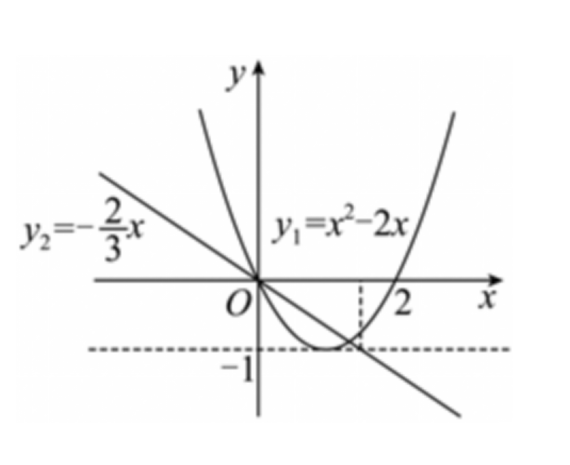
\includegraphics[width=0.24\textwidth]{figures/gao102_q7.png}
\end{center}
\step{当 $m>\dfrac32$ 时，当 $x>m$ 时 $f(x)\in\left(-\infty,-\dfrac23m\right)$，当 $x\leqslant m$ 时 $f(x)\in[-1,+\infty)$，}
\step{显然 $-\dfrac23m<-1$，此时函数 $f(x)$ 的值域不为 $R$，不符合题意；}
\step{当 $m<0$ 时，当 $x>m$ 时，$f(x)\in\left(-\infty,-\dfrac23m\right)$，}
\step{当 $x\leqslant m$ 时，$f(x)\in[m^2-2m,+\infty)$，}
\step{此时 $m^2-2m-\left(-\dfrac23m\right)=m^2-\dfrac43m=m\left(m-\dfrac43\right)>0$，即 $m^2-2m>-\dfrac23m$，}
\step{此时函数 $f(x)$ 的值域不为 $R$，不符合题意；}
\step{当 $0\leqslant m\leqslant\dfrac43$ 时，在 $x\in(0,m)$ 时 $y_2>y_1$，即 $m^2-2m<-\dfrac23m$，}
\step{此时 $f(x)$ 的值域为 $R$，符合题意，}
\step{当 $\dfrac43<m\leqslant\dfrac32$ 时，当 $x>m$ 时，$f(x)\in\left(-\infty,-\dfrac23m\right)$，}
\step{当 $x\leqslant m$ 时，$f(x)\in[-1,+\infty)$，}
\step{此时 $-1-\left(-\dfrac23m\right)=\dfrac23m-1\leqslant0$，即 $-1\leqslant-\dfrac23m$，}
\step{此时函数 $f(x)$ 的值域为 $R$，符合题意；}
\step{综上，$0\leqslant m\leqslant\dfrac32$，即实数 $m$ 的取值范围是 $\left[0,\dfrac32\right]$.}
\solend

\fi

\item 已知函数 $f(x)=x^2-2ax+b$（$a>1$）的定义域和值域都为 $[1,a]$，则 $b=$\blankline[4.4em].

\ifanswer
\solbegin
\step{$f(x)=x^2-2ax+b$（$a>1$）在 $[1,a]$ 严格减，}
\step{则 $f(1)=1-2a+b=a,f(a)=-a^2+b=1$，解得 $a=2,b=5$，所以 $b=5$.}
\solend

\fi

\item 若 $f(x)$ 满足 $f(x+y)=f(x)f(y)$，当 $x>0$ 时，$f(x)$ 的值域为 $(1,+\infty)$，则 $x<0$ 时，
$f(x)$ 的取值范围为\blankline[4.4em].

\ifanswer
\solbegin
\step{因为 $f(x+y)=f(x)f(y)$，令 $x=1$，$y=0$，得 $f(1+0)=f(1)f(0)$，}
\step{又因为当 $x>0$ 时，$f(x)>1$，所以 $f(1)>1>0$，故 $f(0)=1$.}
\step{当 $x<0$ 时，$-x>0$，令 $y=-x$，得 $f(x-x)=f(0)=1=f(x)f(-x)$，}
\step{故 $f(x)=\dfrac1{f(-x)}\in(0,1)$，故 $x<0$ 时，$f(x)$ 的取值范围为 $(0,1)$.}
\solend

\fi

\item 设函数 $f(x)=\begin{cases}x^2+x, & x<0\\ -x^2, & x\geqslant0\end{cases}$，若 $f(f(a))\leqslant2$，则实数 $a$ 的取值范围是\blankline[4.4em].

\ifanswer
\solbegin
\step{函数 $f(x)=\begin{cases}x^2+x, & x<0\\ -x^2, & x\geqslant0\end{cases}$，它的图象如图所示：}
\begin{center}
% 原图第 4 页解析插图直接裁取（原卷排于解析行右侧）。
% 裁框取图形区域，已去粉色水印转灰度。
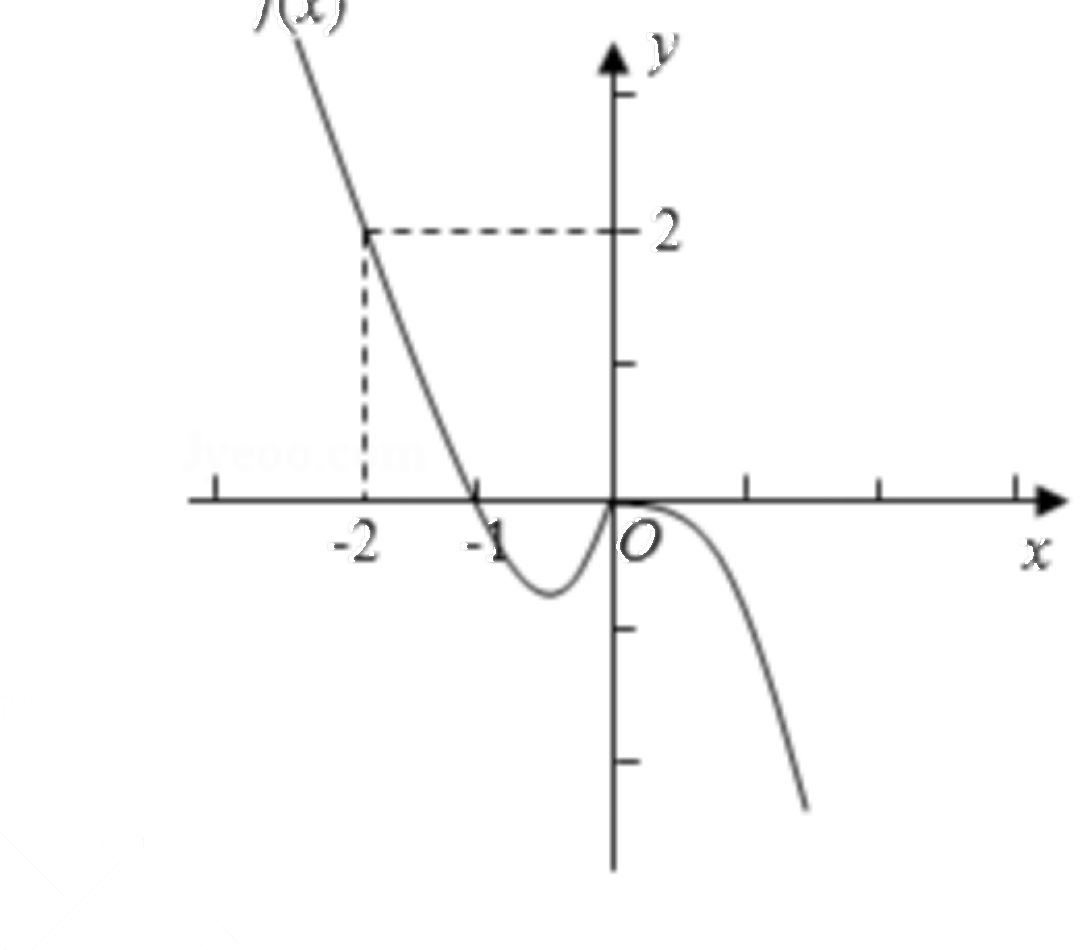
\includegraphics[width=0.30\textwidth]{figures/gao102_q10.png}
\end{center}
\step{由 $f(f(a))\leqslant2$，得 $f(a)\geqslant-2$.}
\step{当 $a<0$ 时，$f(a)=a^2+a=\left(a+\dfrac12\right)^2-\dfrac14\geqslant-2$ 恒成立；}
\step{当 $a\geqslant0$ 时，$f(a)=-a^2\geqslant-2$，即 $a^2\leqslant2$，解得 $0\leqslant a\leqslant\sqrt2$，}
\step{则实数 $a$ 的取值范围是 $(-\infty,\sqrt2]$.}
\solend

\fi

\item 已知二次函数 $f(x)$、$g(x)$ 的二次项系数均为 1，且满足
$\dfrac{f(2025)}{g(2025)}=\dfrac{f(2026)}{g(2026)}=\dfrac{2026}{2025}$，
则 $2026g(2027)-2025f(2027)$ 的值为\blankline[4.4em].

\ifanswer
\solbegin
\step{令 $h(x)=2026g(x)-2025f(x)$，其二次项系数为 $2026-2025=1$.}
\step{由比例条件得 $h(2025)=h(2026)=0$，}
\step{因此 $h(x)=(x-2025)(x-2026),h(2027)=2\times1=2$.}
\solend

\fi

\item 已知函数 $f(x)=\left\lvert x+\dfrac1x-a\right\rvert+1$，对任意实数 $x_1$、$x_2$、$x_3\in\left[\dfrac13,3\right]$，使得以
$f(x_1)$、$f(x_2)$、$f(x_3)$ 数值为边长可构成三角形，则实数 $a$ 的取值范围为\blankline[4.4em].

\ifanswer
\solbegin
\step{对任意实数 $x_1,x_2,x_3\in\left[\dfrac13,3\right]$，}
\step{使得以 $f(x_1)$、$f(x_2)$、$f(x_3)$ 数值为边长可构成三角形，}
\step{只需 $2f(x)_{\min}>f(x)_{\max}$，设 $g(x)=x+\dfrac1x-a$，}
\step{当 $x\in\left[\dfrac13,1\right)$ 时，函数 $g(x)$ 严格减，当 $x\in(1,3]$ 时，函数 $g(x)$ 严格增，}
\step{因为 $g(1)=2-a,g(3)=\dfrac{10}3-a,g\left(\dfrac13\right)=\dfrac{10}3-a$，所以 $g(x)\in\left[2-a,\dfrac{10}3-a\right]$，}
\step{当 $2-a\geqslant0$ 时，即 $a\leqslant2$ 时，$f(x)=\left\lvert x+\dfrac1x-a\right\rvert+1=g(x)+1$，}
\step{此时 $f(x)\in\left[3-a,\dfrac{13}3-a\right]$，}
\step{因此由 $2f(x)_{\min}>f(x)_{\max}\Rightarrow2(3-a)>\dfrac{13}3-a\Rightarrow a<\dfrac53$，而 $a\leqslant2$，所以 $a<\dfrac53$；}
\step{当 $\dfrac{10}3-a\leqslant0$，即 $a\geqslant\dfrac{10}3$ 时，$f(x)=\left\lvert x+\dfrac1x-a\right\rvert+1=-g(x)+1$，}
\step{此时 $f(x)\in\left[a-\dfrac73,a-1\right]$，}
\step{因此由 $2f(x)_{\min}>f(x)_{\max}\Rightarrow2\left(a-\dfrac73\right)>a-1\Rightarrow a>\dfrac{11}3$，而 $a\geqslant\dfrac{10}3$，所以 $a>\dfrac{11}3$，}
\step{若 $2-a<0<\dfrac{10}3-a$ 时，即 $2<a<\dfrac{10}3$ 时，}
\step{若 $a-2\geqslant\dfrac{10}3-a\Rightarrow a\geqslant\dfrac83$，即当 $\dfrac83\leqslant a<\dfrac{10}3$ 时，}
\step{显然此时 $f(x)_{\min}=1$，$f(x)_{\max}=a-2+1=a-1$，}
\step{由 $2f(x)_{\min}>f(x)_{\max}\Rightarrow2\times1>a-1\Rightarrow a<3$，显然 $\dfrac83\leqslant a<3$，}
\step{若 $a-2<\dfrac{10}3-a\Rightarrow a<\dfrac83$，即当 $2<a<\dfrac83$ 时，}
\step{显然此时 $f(x)_{\min}=1,f(x)_{\max}=\dfrac{10}3-a+1=\dfrac{13}3-a$，}
\step{因此由 $2f(x)_{\min}>f(x)_{\max}\Rightarrow2\times1>\dfrac{13}3-a\Rightarrow a>\dfrac73$，而 $\dfrac73<a<\dfrac83$，}
\step{综上，实数 $a$ 的取值范围为 $\left(-\infty,\dfrac53\right)\cup\left(\dfrac73,3\right)\cup\left(\dfrac{11}3,+\infty\right)$.}
\solend

\fi

\end{enumerate}

\bigsec{二、选择题}

\begin{enumerate}
\setcounter{enumi}{12}

\item 已知 $f(x)$ 是定义在 $\R$ 上的奇函数，$g(x)$ 是定义在 $\R$ 上的偶函数，则\mbox{（\quad）}

\keepwithprev
A. $f(x)g(x)$ 是偶函数\qquad B. $f(g(x))$ 是奇函数

C. $f(x)-g(x)$ 是奇函数\qquad D. $g(f(x))$ 是偶函数

\ifanswer
\solbegin
\step{$g(f(x))$ 的定义域为 $\R$，且 $g(f(-x))=g(-f(x))=g(f(x))$，}
\step{所以 $g(f(x))$ 是偶函数，故选 $D$.}
\solend

\fi

\item 已知定义在 $R$ 上的偶函数 $f(x)=\lvert x-m+1\rvert-2$，若正实数 $a$、$b$ 满足 $f(a)+f(2b)=m$，
则 $\dfrac1a+\dfrac2b$ 的最小值为\mbox{（\quad）}

\keepwithprev
A. $\dfrac95$\qquad\qquad B. $9$\qquad\qquad C. $\dfrac85$\qquad\qquad D. $8$

\ifanswer
\solbegin
\step{因为 $f(x)=\lvert x-m+1\rvert-2$ 是偶函数，所以 $-m+1=0$，所以 $m=1$，}
\step{所以 $f(x)=\lvert x\rvert-2$，若正实数 $a$、$b$ 满足 $f(a)+f(2b)=m$，}
\step{则 $a-2+2b-2=1$，所以 $a+2b=5$，}
\step{所以 $\dfrac1a+\dfrac2b=\dfrac15(a+2b)\left(\dfrac1a+\dfrac2b\right)=\dfrac15\left(5+\dfrac{2a}b+\dfrac{2b}a\right)\geqslant\dfrac95$，}
\step{当且仅当 $a=b=\dfrac53$ 时取等号，则 $\dfrac1a+\dfrac2b$ 的最小值为 $\dfrac95$，故选 $A$.}
\solend

\fi

\item 设函数 $g(x)=x^2-2$（$x\in\R$），$f(x)=\begin{cases}g(x)+x+4, & x<g(x)\\ g(x)-x, & x\geqslant g(x)\end{cases}$，则 $f(x)$ 的值域是

\mbox{（\quad）}

\keepwithprev
A. $\left[-\dfrac94,0\right]\cup(1,+\infty)$\qquad\qquad B. $[0,+\infty)$

C. $\left[-\dfrac94,+\infty\right)$\qquad\qquad D. $\left[-\dfrac94,0\right]\cup(2,+\infty)$

\ifanswer
\solbegin
\step{当 $x<g(x)$，即 $x<x^2-2$，$(x-2)(x+1)>0$ 时，$x>2$ 或 $x<-1$，}
\step{$f(x)=g(x)+x+4=x^2-2+x+4=x^2+x+2=(x+0.5)^2+1.75$，}
\step{其最小值趋向于 $f(-1)$ 即 2，无最大值，}
\step{因此这个区间的值域为 $(2,+\infty)$.}
\step{当 $x\geqslant g(x)$ 时，$-1\leqslant x\leqslant2$，$f(x)=g(x)-x=x^2-2-x=(x-0.5)^2-2.25$，}
\step{其最小值为 $f(0.5)=-2.25$，其最大值为 $f(2)=0$，}
\step{因此这区间的值域为 $[-2.25,0]$.}
\step{综上，函数值域为 $\left[-\dfrac94,0\right]\cup(2,+\infty)$，故选 $D$.}
\solend

\fi

\item 设 $D$ 是含数 1 的有限实数集，$f(x)$ 是定义在 $D$ 上的函数，若 $f(x)$ 的图象绕原点逆时针
旋转 $\dfrac{\pi}{6}$ 与原图象重合，则在以下各项中，$f(1)$ 的可能取值只能是\mbox{（\quad）}

\keepwithprev
A. $\sqrt3$\qquad\qquad B. $\dfrac{\sqrt3}2$\qquad\qquad C. $\dfrac{\sqrt3}3$\qquad\qquad D. $0$

\ifanswer
\solbegin
\step{问题相当于圆上由 12 个点为一组，每次绕原点逆时针旋转 $\dfrac{\pi}{6}$ 个单位后与下一个点}
\step{会重合。我们可以通过代入和赋值的方法，当 $f(1)=\sqrt3$、$\dfrac{\sqrt3}3$、$0$ 时，}
\step{此时得到的圆心角为 $\dfrac{\pi}{3}$、$\dfrac{\pi}{6}$、$0$，然而此时 $x=0$ 或者 $x=1$ 时，}
\step{都有 2 个 $y$ 与之对应，而我们知道函数的定义就是要求一个 $x$ 只能对应一个 $y$，}
\step{因此只有当 $x=\dfrac{\sqrt3}2$，此时旋转 $\dfrac{\pi}{6}$，此时满足一个 $x$ 只会对应一个 $y$，故选 $B$.}
\solend

\fi

\end{enumerate}

\bigsec{三、解答题}

\begin{enumerate}
\setcounter{enumi}{16}

\item 求下列函数的值域.

（1）$y=\dfrac{2x^2-3x+5}{x-1}\left(x\in\left[\dfrac32,3\right]\right)$；

（2）$f(x)=\sqrt{x}-\sqrt{2-x}+\sqrt{x(2-x)}$.

\ansspace*[10]

\ifanswer
\solbegin
\stepm{（1）}{令 $t=x-1$，则 $t\in\left[\dfrac12,2\right]$，原函数化为 $Y(t)=2t+\dfrac4t+1$.}
\step{当 $0<u<v$ 时，$Y(v)-Y(u)=2(v-u)\left(1-\dfrac2{uv}\right)$，}
\step{所以 $Y$ 在 $\left[\dfrac12,\sqrt2\right]$ 上严格递减，在 $[\sqrt2,2]$ 上严格递增.}
\step{由 $Y(\sqrt2)=4\sqrt2+1,Y\left(\dfrac12\right)=10,Y(2)=7$，得值域为 $[4\sqrt2+1,10]$.}
\stepm{（2）}{定义域为 $[0,2]$.}
\step{令 $s=\sqrt{x}-\sqrt{2-x}$，$\sqrt{x}$ 与 $-\sqrt{2-x}$ 均随 $x$ 严格递增，}
\step{$s$ 从 $-\sqrt2$ 递增到 $\sqrt2$，即 $s\in[-\sqrt2,\sqrt2]$.}
\step{由 $s^2=2-2\sqrt{x(2-x)}$，得 $f(x)=s+\dfrac{2-s^2}2=-\dfrac12(s-1)^2+\dfrac32$.}
\step{当 $s=1$ 时取得最大值 $\dfrac32$；当 $s=-\sqrt2$ 时取得最小值 $-\sqrt2$；}
\step{因此值域为 $\left[-\sqrt2,\dfrac32\right]$.}
\solend

\fi

\item 已知 $f(2x+1)=\dfrac{2x+1}{x+1}$.

（1）解不等式 $f(x)<x$；

（2）求 $f(1)+f(2)+\cdots+f(6)+f\left(\dfrac12\right)+f\left(\dfrac13\right)+\cdots+f\left(\dfrac16\right)$ 的值.

\ansspace*[12]

\ifanswer
\solbegin
\step{令 $t=2x+1$，则 $x=\dfrac{t-1}2$，得 $f(t)=\dfrac{2t}{t+1},t\neq-1$.}
\stepm{（1）}{不等式等价于 $\dfrac{2x}{x+1}<x\Leftrightarrow\dfrac{x(x-1)}{x+1}>0$.}
\step{以 $-1,0,1$ 分区间判断符号，得解集为 $(-1,0)\cup(1,+\infty)$.}
\stepm{（2）}{当 $x>0$ 时，$f(x)+f\left(\dfrac1x\right)=\dfrac{2x}{x+1}+\dfrac2{x+1}=2$.}
\step{将 $f(2),\cdots,f(6)$ 分别与其倒数对应的函数值配对，共 5 对，且 $f(1)=1$，}
\step{因此原式$=1+5\times2=11$.}
\solend

\fi

\item 已知函数 $f(x)$、$g(x)$ 是定义在 $R$ 上的函数，其中 $f(x)$ 是奇函数，$g(x)$ 是偶函数，且
$f(x)+g(x)=ax^2-x$.

（1）求 $f(x)$ 和 $g(x)$ 的解析式；

（2）$h(x)=f(x)+g(x)+(1-a)x^2-2ax+4$ 在 $[1,3]$ 上有两个零点，求实数 $a$ 的取值范
围.

\ansspace*[14]

\ifanswer
\solbegin
\stepm{（1）}{因为 $f(x)+g(x)=ax^2-x$①，所以 $f(-x)+g(-x)=ax^2+x$，}
\step{又 $f(x)$ 是奇函数，$g(x)$ 是偶函数，}
\step{所以 $f(-x)=-f(x)$，$g(-x)=g(x)$，}
\step{所以 $-f(x)+g(x)=ax^2+x$②，}
\step{联立①②解得 $f(x)=-x$，$g(x)=ax^2$.}
\stepm{（2）}{$h(x)=f(x)+g(x)+(1-a)x^2-2ax+4$}
\step{$=ax^2-x+(1-a)x^2-2ax+4=x^2-(2a+1)x+4$，}
\step{是开口向上，对称轴为 $x=\dfrac{2a+1}2$ 的二次函数，}
\step{因为 $h(x)$ 在 $[1,3]$ 上有两个零点，所以 $\begin{cases}\Delta=(2a+1)^2-16>0\\ 1<\dfrac{2a+1}2<3\\ h(1)=1-(2a+1)+4\geqslant0\\ h(3)=9-3(2a+1)+4\geqslant0\end{cases}$，}
\step{解得 $\dfrac32<a\leqslant\dfrac53$，故实数 $a$ 的取值范围为 $\left(\dfrac32,\dfrac53\right]$.}
\solend

\fi

\item 若函数 $f(x)$ 在区间 $[a,b]$ 上的值域恰为 $\left[\dfrac1b,\dfrac1a\right]$，则称区间 $[a,b]$ 为 $f(x)$ 的一个“倒域
区间”。已知定义在 $[-4,4]$ 上的奇函数 $g(x)$，当 $x\in[0,4]$ 时，$g(x)=-x^2+2x$.

（1）求 $g(x)$ 的解析式；

（2）若关于 $x$ 的方程 $g(x)=-mx-m$ 在 $(0,4)$ 上恰有两个不相等的实数根，求实数 $m$ 的
取值范围；

（3）求函数 $g(x)$ 在 $[-4,0]$ 内的“倒域区间”.

\ansspace*[16]

\ifanswer
\solbegin
\stepm{（1）}{当 $x\in[-4,0)$ 时，$-x\in(0,4]$，}
\step{由奇函数的定义得 $g(x)=-g(-x)=-[(-x)^2+2(-x)]=x^2+2x$，}
\step{所以 $g(x)=\begin{cases}-x^2+2x, & 0\leqslant x\leqslant4\\ x^2+2x, & -4\leqslant x<0\end{cases}$.}
\stepm{（2）}{方程 $g(x)=-mx-m$，即 $x^2-(m+2)x-m=0$，}
\step{设 $h(x)=x^2-(m+2)x-m$，$0<x<4$，}
\step{由题意得 $\begin{cases}h(0)=-m>0\\ h(4)=8-5m>0\\ \Delta=(m+2)^2+4m>0\\ 0<\dfrac{m+2}2<4\end{cases}$，解得 $2\sqrt3-4<m<0$，}
\step{即实数 $m$ 的取值范围是 $(2\sqrt3-4,0)$.}
\stepm{（3）}{易得当 $-4\leqslant a<b<0$ 时，$\dfrac1b<\dfrac1a$，}
\step{且 $g(x)$ 在 $[-4,-1]$ 上严格减，在 $[-1,0]$ 上严格增，}
\step{故当 $x\in[-4,0]$ 时，$g(x)_{\min}=g(-1)=-1$，}
\step{所以 $\dfrac1b\geqslant-1$，所以 $-4<b\leqslant-1$，所以 $-4\leqslant a<b\leqslant-1$，}
\step{则 $\begin{cases}g(a)=a^2+2a=\dfrac1a\\ g(b)=b^2+2b=\dfrac1b\\ -4\leqslant a<b\leqslant-1\end{cases}$，解得 $\begin{cases}a=-\dfrac{1+\sqrt5}2\\ b=-1\end{cases}$，}
\step{所以 $g(x)$ 在 $[-4,0]$ 内的“倒域区间”为 $\left[-\dfrac{1+\sqrt5}2,-1\right]$.}
\solend

\fi

\item 我们知道：函数 $y=f(x)$ 的图象关于坐标原点成中心对称图形的充要条件是函数
$y=f(x)$ 为奇函数。有同学发现可以推广为：函数 $y=f(x)$ 的图象关于点 $(a,b)$ 成中心对
称图形的充要条件为函数 $y=f(x+a)-b$ 为奇函数。已知函数 $f(x)=\dfrac{2x}{3-x}$.

（1）求函数 $f(x)$ 图象的对称中心；

（2）若定义在 $R$ 上的函数 $y=g(x)$ 的图象关于点 $(1,2)$ 对称，且 $g(1)=2$，当 $x\in[0,1)$
时，$g(x)=x^2-tx+t+1$.

（$i$）求 $g(-3)+g(5)$ 的值；

（$ii$）若对$\forall x_1\in[0,2]$，$\exists x_2\in[-3,2]$ 使得 $g(x_1)=f(x_2)$ 恒成立，求实数 $t$ 的取值范围.

\ansspace*[18]

\ifanswer
\solbegin
\stepm{（1）}{由 $f(x)=\dfrac{2x}{3-x}=-2+\dfrac6{3-x}$，}
\step{易得 $f(x+3)+2=-2+\dfrac6{3-(x+3)}+2=-\dfrac6x$ 为奇函数，}
\step{$f(x)$ 的图象关于 $(3,-2)$ 对称.}
\stepm{（2）}{（$i$）$y=g(x)$ 图象关于点 $(1,2)$ 对称，则 $g(1+x)+g(1-x)=4$，}
\step{令 $x=4$，则 $g(-3)+g(5)=4$.}
\step{（$ii$）有 $g(x)$ 在 $x\in[0,2]$ 的取值范围为 $f(x)$ 在 $x\in[-3,2]$ 的取值范围的}
\step{子集，}
\step{因为 $f(x)=\dfrac{2x}{3-x}=\dfrac{6-2(3-x)}{3-x}=\dfrac6{3-x}-2$ 在 $[-3,2]$ 上严格增，}
\step{所以 $f(x)$ 在 $x\in[-3,2]$ 上的取值范围为 $[-1,4]$，}
\step{记 $g(x)$ 的值域为 $A$，且 $g(1)=2$，当 $x\in[0,1)$ 时 $g(x)=x^2-tx+t+1$，}
\step{①当 $\dfrac t2\leqslant0$，即 $t\leqslant0$ 时，有 $g(x)$ 在 $[0,1)$ 上严格增，}
\step{由对称性得 $g(x)$ 在 $[1,2]$ 上严格增，故 $g(x)$ 在 $[0,2]$ 上严格增，}
\step{故 $g(x)_{\min}=g(0)=t+1$，$g(x)_{\max}=g(2)=4-(t+1)=3-t$，$t\leqslant0$，}
\step{则 $A=[t+1,3-t]\subseteq[-1,4]$，即 $\begin{cases}t\leqslant0\\ t+1\geqslant-1\\ 3-t\leqslant4\end{cases}$，解得 $-1\leqslant t\leqslant0$.}
\step{②当 $0<\dfrac t2<1$，即 $0<t<2$ 时，}
\step{$g(x)$ 在 $\left(0,\dfrac t2\right)$ 上严格减，在 $\left(\dfrac t2,1\right)$ 上严格增，}
\step{由对称性得 $g(x)$ 在 $\left(2-\dfrac t2,2\right)$ 上严格减，在 $\left(1,2-\dfrac t2\right)$ 上严格增，}
\step{故 $g(x)$ 在 $\left(0,\dfrac t2\right)$ 上严格减，在 $\left(\dfrac t2,2-\dfrac t2\right)$ 上严格增，}
\step{在 $\left(2-\dfrac t2,2\right)$ 上严格减，则 $A=\left[g\left(\dfrac t2\right),g\left(2-\dfrac t2\right)\right]$，}
\step{由 $0<t<2$，得 $g(0)=t+1\in(1,3)$，$g(2)=4-(t+1)=3-t\in(1,3)$，}
\step{$g\left(\dfrac t2\right)=-\dfrac{t^2}4+t+1=-\dfrac14(t-2)^2+2\in(1,2]$，}
\step{又 $g\left(\dfrac t2\right)+g\left(2-\dfrac t2\right)=4$，$g\left(2-\dfrac t2\right)\in(2,3)$，}
\step{当 $0<t<2$ 时，$A\subseteq[-1,4]$ 恒成立，}
\step{③当 $\dfrac t2\geqslant1$，即 $t\geqslant2$ 时，有 $g(x)$ 在 $[0,1)$ 上严格减，}
\step{由对称点 $(1,2)$ 得 $g(x)$ 在 $[1,2]$ 上严格减，所以 $g(x)$ 在 $[0,2]$ 上严格减，}
\step{故 $g(x)_{\max}=g(0)=t+1$，$g(x)_{\min}=g(2)=4-(t+1)=3-t$，$t\geqslant2$，}
\step{则 $A=[3-t,t+1]\subseteq[-1,4]$，即 $\begin{cases}t\geqslant2\\ t+1\leqslant4\\ 3-t\geqslant-1\end{cases}$，解得 $2\leqslant t\leqslant3$.}
\step{综上，$t$ 的范围为 $\{t\mid-1\leqslant t\leqslant3\}$.}
\solend

\fi

\end{enumerate}

\end{document}
"
% 紧凑版：xelatex "\def\iscompact{1}% 高一102_华师大二附中_周末作业5.tex
%   —— 高一上数学“2026-2027 年华师大二附中高一上周末作业 5”（试卷版/答案版）
% 试卷版：xelatex 高一102_华师大二附中_周末作业5.tex
% 答案版：xelatex "\def\isanswer{1}\input{高一102_华师大二附中_周末作业5.tex}"
% 紧凑版：xelatex "\def\iscompact{1}\input{高一102_华师大二附中_周末作业5.tex}"
%
% 原始材料：微信公众号“魔都数学加油站”文章，作者破晓，2026-11-01 21:56 发布；
% 连载“27学年高一102”，原文标题“27学年高一102——2026-2027年上海市华师大二附中高一上周末作业5函数”；
% 原文链接：https://mp.weixin.qq.com/s/CDvOCcxFskIe9aFUeKi3Ww。
% 正文为 13 张 PNG 页（第 1、2、10、13 页 2560×3620，其余 4762×6735），题目下印有【解析】，为讲评版。
% 题目、解析均据原图转录；卷面水印及公众号页脚未录入。
%
% 卷首标题：原卷印作“2026-2027 年华师大二附中高一上周末作业 5”（公众号标题中的“上海市”“函数”
% 卷面标题行没有，本稿照卷面），年份区间按全稿惯例排 en dash；原卷未印副标题，本稿按题目内容
% 标为“函数”（全稿首份以函数为单一模块的卷子）。
%
% 与原卷的排版差异：
%   ① 原文从第 3 题起，填空题编号为 3—12、选择题为 13—16、解答题为 17—21，本稿保留原题号；
%   ② 原卷每题下直接印【解析】，本稿按全稿惯例将解析置于答案版；选择题括号内未印答案，另由
%      解析末句“故选 X”给出；
%   ③ 原卷未印副标题，本稿按“知识模块”口径补出；
%   ④ 原卷填空横线按全稿惯例排为 \blankline[4.4em]；解答题按惯例加 \ansspace；选择题括号排
%      \mbox{（\quad）}、选项段前按惯例加 \keepwithprev；
%   ⑤ 原卷 $f(x)_{min}$、$f(x)_{max}$ 等下标排斜体，按 高一96 成例改正体 $\min$、$\max$；
%   ⑥ 原卷数集排斜体 $R$（第 13 题排粗体），按全稿惯例改 $\R$；
%   ⑦ 第 7、10 两题的解析插图裁自原图（去粉色水印转灰度），仅答案版显示。
%
% 原卷存疑／笔误（均照录加注）：
%   第 3 题解析“减去都对应 −2 和 2 的”措辞含糊（意为减去恒取 −2 与恒取 2 的两个常函数）；
%   第 15 题解析“其最小值趋向于 f(−1) 即 2”（该段 f(x)=x²+x+2 在 x→−1⁻ 时趋于 2、取不到）；
%   第 16 题解析末句“因此只有当 x=√3/2”（按上下文应为 f(1)=√3/2）；
%   第 16 题解析以 f(1)=√3、√3/3、0 赋值时称“得到的圆心角为 π/3、π/6、0”，其中 √3/3 对应
%   圆心角 π/6 的说法与该点 (1,√3/3) 的实际幅角一致，但与选项 C（√3/3）被排除的结论矛盾
%   （幅角 π/6 的点旋转 π/6 后落到幅角 π/3 处，仍占 12 等分点位，原卷解析未展开），照录。
%
% 行数核对：逐题数 \step/\stepm 条数，合计 155 条（Q3：2；Q4：3；Q5：6；Q6：5；Q7：19；
% Q8：2；Q9：4；Q10：5；Q11：3；Q12：19；Q13：2；Q14：5；Q15：8；Q16：5；Q17：10；
% Q18：6；Q19：10；Q20：13；Q21：28），与原卷印刷行逐题相等。
%
\documentclass[a4paper,11pt]{article}
\usepackage{common}

\begin{document}

\examtitlest[3]{2026--2027 年华师大二附中高一上周末作业 5}{函数}

\bigsec{一、填空题}

\begin{enumerate}
\setcounter{enumi}{2}

\item 已知函数 $y=f(x)$ 的定义域为 $\{-2,-1,1,2\}$，值域为 $\{-2,2\}$，则满足条件的函数
$y=f(x)$ 最多有\blankline[4.4em]个.

\ifanswer
\solbegin
\step{定义域中 4 个元素每个都可以对应 $-2$ 和 $2$ 中的一个，减去都对应 $-2$ 和 $2$ 的，}
\step{则满足条件的函数 $y=f(x)$ 最多有 $2^4-2=14$.}
\solend

\fi

\item 已知函数 $f(2x)$ 的定义域为 $[-2,2]$，则函数 $f(x-3)$ 的定义域为\blankline[4.4em].

\ifanswer
\solbegin
\step{因为函数 $f(2x)$ 的定义域为 $[-2,2]$，即 $-2\leqslant x\leqslant2$，所以 $-4\leqslant2x\leqslant4$，}
\step{得 $f(x)$ 的定义域为 $[-4,4]$，由 $-4\leqslant x-3\leqslant4$，解得 $-1\leqslant x\leqslant7$，}
\step{即函数 $f(x-3)$ 的定义域为 $[-1,7]$.}
\solend

\fi

\item 函数 $f(x)=\begin{cases}-x-1, & x<0\\ -x+1, & x>0\end{cases}$，则 $f(x)-f(-x)>1$ 的解集为\blankline[4.4em].

\ifanswer
\solbegin
\step{定义域为 $\{x\mid x\neq0\}$.}
\step{当 $x<0$ 时，$-x>0,f(-x)=x+1$，}
\step{$f(x)-f(-x)=(-x-1)-(x+1)=-2x-2>1$，得 $x<-\dfrac32$.}
\step{当 $x>0$ 时，$f(-x)=x-1,f(x)-f(-x)=(-x+1)-(x-1)=-2x+2>1$，}
\step{得 $0<x<\dfrac12$.}
\step{故解集为 $\left(-\infty,-\dfrac32\right)\cup\left(0,\dfrac12\right)$.}
\solend

\fi

\item 已知函数 $f(x)=x^2-2(m-3)x+5$ 在区间 $[2,+\infty)$ 上的最小值为 1，则实数 $m=$\blankline[4.4em].

\ifanswer
\solbegin
\step{函数 $f(x)$ 图象的对称轴为 $x=m-3$.}
\step{当 $m-3\leqslant2$，即 $m\leqslant5$ 时，$f(x)_{\min}=f(2)=9-4m+12=1$，解得 $m=5$；}
\step{当 $m-3>2$，即 $m>5$ 时，$f(x)_{\min}=f(m-3)=-m^2+6m-4=1$，}
\step{解得 $m=5$（舍去）或 $1$（舍去），}
\step{综上，$m=5$.}
\solend

\fi

\item 已知函数 $f(x)=\begin{cases}x^2-2x, & x\leqslant m\\ -\dfrac23x, & x>m\end{cases}$ 的值域为 $R$，则实数 $m$ 的取值范围是\blankline[4.4em].

\ifanswer
\solbegin
\step{对于函数 $y_1=x^2-2x$，则 $y_1=(x-1)^2-1\geqslant-1$，当且仅当 $x=1$ 时取等号，}
\step{且函数在 $(-\infty,1)$ 上严格减，在 $(1,+\infty)$ 上严格增，}
\step{对于函数 $y_2=-\dfrac23x$，令 $y_2=-1$，则 $x=\dfrac32$，且函数在定义域上严格减，}
\step{令 $x^2-2x=-\dfrac23x$，解得 $x=0$ 或 $x=\dfrac43$，}
\step{所以 $y_2=-\dfrac23x$ 与 $y_1=x^2-2x$ 的两个交点分别为 $(0,0)$、$\left(\dfrac43,-\dfrac89\right)$，}
\step{则函数 $y_2=-\dfrac23x$ 与 $y_1=x^2-2x$ 的图象如图所示：}
\begin{center}
% 原图第 2 页解析插图直接裁取（原卷排于解析行右侧）。
% 裁框取图形区域，已去粉色水印转灰度。
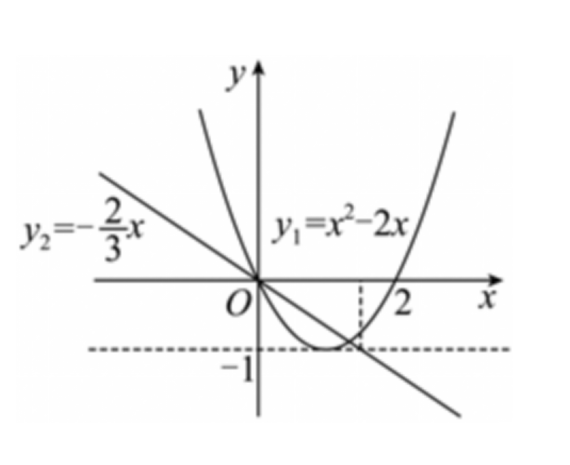
\includegraphics[width=0.24\textwidth]{figures/gao102_q7.png}
\end{center}
\step{当 $m>\dfrac32$ 时，当 $x>m$ 时 $f(x)\in\left(-\infty,-\dfrac23m\right)$，当 $x\leqslant m$ 时 $f(x)\in[-1,+\infty)$，}
\step{显然 $-\dfrac23m<-1$，此时函数 $f(x)$ 的值域不为 $R$，不符合题意；}
\step{当 $m<0$ 时，当 $x>m$ 时，$f(x)\in\left(-\infty,-\dfrac23m\right)$，}
\step{当 $x\leqslant m$ 时，$f(x)\in[m^2-2m,+\infty)$，}
\step{此时 $m^2-2m-\left(-\dfrac23m\right)=m^2-\dfrac43m=m\left(m-\dfrac43\right)>0$，即 $m^2-2m>-\dfrac23m$，}
\step{此时函数 $f(x)$ 的值域不为 $R$，不符合题意；}
\step{当 $0\leqslant m\leqslant\dfrac43$ 时，在 $x\in(0,m)$ 时 $y_2>y_1$，即 $m^2-2m<-\dfrac23m$，}
\step{此时 $f(x)$ 的值域为 $R$，符合题意，}
\step{当 $\dfrac43<m\leqslant\dfrac32$ 时，当 $x>m$ 时，$f(x)\in\left(-\infty,-\dfrac23m\right)$，}
\step{当 $x\leqslant m$ 时，$f(x)\in[-1,+\infty)$，}
\step{此时 $-1-\left(-\dfrac23m\right)=\dfrac23m-1\leqslant0$，即 $-1\leqslant-\dfrac23m$，}
\step{此时函数 $f(x)$ 的值域为 $R$，符合题意；}
\step{综上，$0\leqslant m\leqslant\dfrac32$，即实数 $m$ 的取值范围是 $\left[0,\dfrac32\right]$.}
\solend

\fi

\item 已知函数 $f(x)=x^2-2ax+b$（$a>1$）的定义域和值域都为 $[1,a]$，则 $b=$\blankline[4.4em].

\ifanswer
\solbegin
\step{$f(x)=x^2-2ax+b$（$a>1$）在 $[1,a]$ 严格减，}
\step{则 $f(1)=1-2a+b=a,f(a)=-a^2+b=1$，解得 $a=2,b=5$，所以 $b=5$.}
\solend

\fi

\item 若 $f(x)$ 满足 $f(x+y)=f(x)f(y)$，当 $x>0$ 时，$f(x)$ 的值域为 $(1,+\infty)$，则 $x<0$ 时，
$f(x)$ 的取值范围为\blankline[4.4em].

\ifanswer
\solbegin
\step{因为 $f(x+y)=f(x)f(y)$，令 $x=1$，$y=0$，得 $f(1+0)=f(1)f(0)$，}
\step{又因为当 $x>0$ 时，$f(x)>1$，所以 $f(1)>1>0$，故 $f(0)=1$.}
\step{当 $x<0$ 时，$-x>0$，令 $y=-x$，得 $f(x-x)=f(0)=1=f(x)f(-x)$，}
\step{故 $f(x)=\dfrac1{f(-x)}\in(0,1)$，故 $x<0$ 时，$f(x)$ 的取值范围为 $(0,1)$.}
\solend

\fi

\item 设函数 $f(x)=\begin{cases}x^2+x, & x<0\\ -x^2, & x\geqslant0\end{cases}$，若 $f(f(a))\leqslant2$，则实数 $a$ 的取值范围是\blankline[4.4em].

\ifanswer
\solbegin
\step{函数 $f(x)=\begin{cases}x^2+x, & x<0\\ -x^2, & x\geqslant0\end{cases}$，它的图象如图所示：}
\begin{center}
% 原图第 4 页解析插图直接裁取（原卷排于解析行右侧）。
% 裁框取图形区域，已去粉色水印转灰度。
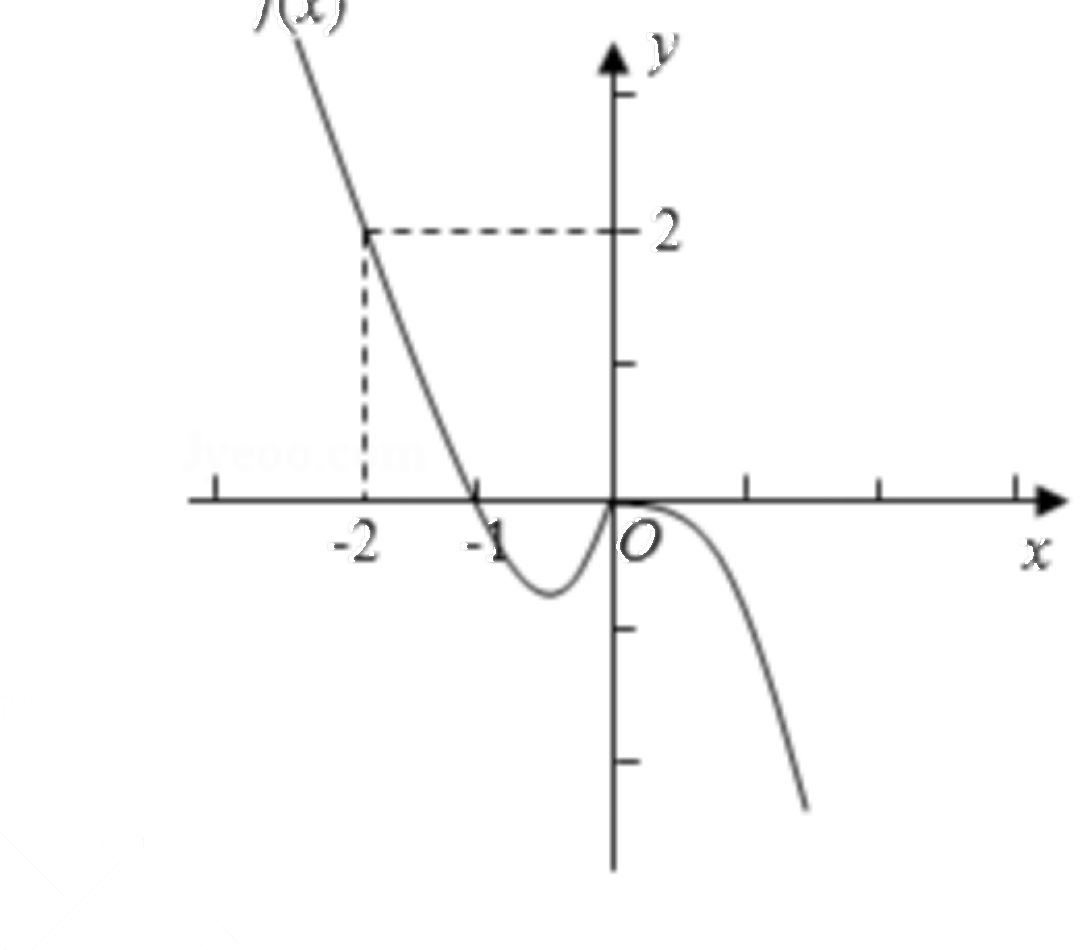
\includegraphics[width=0.30\textwidth]{figures/gao102_q10.png}
\end{center}
\step{由 $f(f(a))\leqslant2$，得 $f(a)\geqslant-2$.}
\step{当 $a<0$ 时，$f(a)=a^2+a=\left(a+\dfrac12\right)^2-\dfrac14\geqslant-2$ 恒成立；}
\step{当 $a\geqslant0$ 时，$f(a)=-a^2\geqslant-2$，即 $a^2\leqslant2$，解得 $0\leqslant a\leqslant\sqrt2$，}
\step{则实数 $a$ 的取值范围是 $(-\infty,\sqrt2]$.}
\solend

\fi

\item 已知二次函数 $f(x)$、$g(x)$ 的二次项系数均为 1，且满足
$\dfrac{f(2025)}{g(2025)}=\dfrac{f(2026)}{g(2026)}=\dfrac{2026}{2025}$，
则 $2026g(2027)-2025f(2027)$ 的值为\blankline[4.4em].

\ifanswer
\solbegin
\step{令 $h(x)=2026g(x)-2025f(x)$，其二次项系数为 $2026-2025=1$.}
\step{由比例条件得 $h(2025)=h(2026)=0$，}
\step{因此 $h(x)=(x-2025)(x-2026),h(2027)=2\times1=2$.}
\solend

\fi

\item 已知函数 $f(x)=\left\lvert x+\dfrac1x-a\right\rvert+1$，对任意实数 $x_1$、$x_2$、$x_3\in\left[\dfrac13,3\right]$，使得以
$f(x_1)$、$f(x_2)$、$f(x_3)$ 数值为边长可构成三角形，则实数 $a$ 的取值范围为\blankline[4.4em].

\ifanswer
\solbegin
\step{对任意实数 $x_1,x_2,x_3\in\left[\dfrac13,3\right]$，}
\step{使得以 $f(x_1)$、$f(x_2)$、$f(x_3)$ 数值为边长可构成三角形，}
\step{只需 $2f(x)_{\min}>f(x)_{\max}$，设 $g(x)=x+\dfrac1x-a$，}
\step{当 $x\in\left[\dfrac13,1\right)$ 时，函数 $g(x)$ 严格减，当 $x\in(1,3]$ 时，函数 $g(x)$ 严格增，}
\step{因为 $g(1)=2-a,g(3)=\dfrac{10}3-a,g\left(\dfrac13\right)=\dfrac{10}3-a$，所以 $g(x)\in\left[2-a,\dfrac{10}3-a\right]$，}
\step{当 $2-a\geqslant0$ 时，即 $a\leqslant2$ 时，$f(x)=\left\lvert x+\dfrac1x-a\right\rvert+1=g(x)+1$，}
\step{此时 $f(x)\in\left[3-a,\dfrac{13}3-a\right]$，}
\step{因此由 $2f(x)_{\min}>f(x)_{\max}\Rightarrow2(3-a)>\dfrac{13}3-a\Rightarrow a<\dfrac53$，而 $a\leqslant2$，所以 $a<\dfrac53$；}
\step{当 $\dfrac{10}3-a\leqslant0$，即 $a\geqslant\dfrac{10}3$ 时，$f(x)=\left\lvert x+\dfrac1x-a\right\rvert+1=-g(x)+1$，}
\step{此时 $f(x)\in\left[a-\dfrac73,a-1\right]$，}
\step{因此由 $2f(x)_{\min}>f(x)_{\max}\Rightarrow2\left(a-\dfrac73\right)>a-1\Rightarrow a>\dfrac{11}3$，而 $a\geqslant\dfrac{10}3$，所以 $a>\dfrac{11}3$，}
\step{若 $2-a<0<\dfrac{10}3-a$ 时，即 $2<a<\dfrac{10}3$ 时，}
\step{若 $a-2\geqslant\dfrac{10}3-a\Rightarrow a\geqslant\dfrac83$，即当 $\dfrac83\leqslant a<\dfrac{10}3$ 时，}
\step{显然此时 $f(x)_{\min}=1$，$f(x)_{\max}=a-2+1=a-1$，}
\step{由 $2f(x)_{\min}>f(x)_{\max}\Rightarrow2\times1>a-1\Rightarrow a<3$，显然 $\dfrac83\leqslant a<3$，}
\step{若 $a-2<\dfrac{10}3-a\Rightarrow a<\dfrac83$，即当 $2<a<\dfrac83$ 时，}
\step{显然此时 $f(x)_{\min}=1,f(x)_{\max}=\dfrac{10}3-a+1=\dfrac{13}3-a$，}
\step{因此由 $2f(x)_{\min}>f(x)_{\max}\Rightarrow2\times1>\dfrac{13}3-a\Rightarrow a>\dfrac73$，而 $\dfrac73<a<\dfrac83$，}
\step{综上，实数 $a$ 的取值范围为 $\left(-\infty,\dfrac53\right)\cup\left(\dfrac73,3\right)\cup\left(\dfrac{11}3,+\infty\right)$.}
\solend

\fi

\end{enumerate}

\bigsec{二、选择题}

\begin{enumerate}
\setcounter{enumi}{12}

\item 已知 $f(x)$ 是定义在 $\R$ 上的奇函数，$g(x)$ 是定义在 $\R$ 上的偶函数，则\mbox{（\quad）}

\keepwithprev
A. $f(x)g(x)$ 是偶函数\qquad B. $f(g(x))$ 是奇函数

C. $f(x)-g(x)$ 是奇函数\qquad D. $g(f(x))$ 是偶函数

\ifanswer
\solbegin
\step{$g(f(x))$ 的定义域为 $\R$，且 $g(f(-x))=g(-f(x))=g(f(x))$，}
\step{所以 $g(f(x))$ 是偶函数，故选 $D$.}
\solend

\fi

\item 已知定义在 $R$ 上的偶函数 $f(x)=\lvert x-m+1\rvert-2$，若正实数 $a$、$b$ 满足 $f(a)+f(2b)=m$，
则 $\dfrac1a+\dfrac2b$ 的最小值为\mbox{（\quad）}

\keepwithprev
A. $\dfrac95$\qquad\qquad B. $9$\qquad\qquad C. $\dfrac85$\qquad\qquad D. $8$

\ifanswer
\solbegin
\step{因为 $f(x)=\lvert x-m+1\rvert-2$ 是偶函数，所以 $-m+1=0$，所以 $m=1$，}
\step{所以 $f(x)=\lvert x\rvert-2$，若正实数 $a$、$b$ 满足 $f(a)+f(2b)=m$，}
\step{则 $a-2+2b-2=1$，所以 $a+2b=5$，}
\step{所以 $\dfrac1a+\dfrac2b=\dfrac15(a+2b)\left(\dfrac1a+\dfrac2b\right)=\dfrac15\left(5+\dfrac{2a}b+\dfrac{2b}a\right)\geqslant\dfrac95$，}
\step{当且仅当 $a=b=\dfrac53$ 时取等号，则 $\dfrac1a+\dfrac2b$ 的最小值为 $\dfrac95$，故选 $A$.}
\solend

\fi

\item 设函数 $g(x)=x^2-2$（$x\in\R$），$f(x)=\begin{cases}g(x)+x+4, & x<g(x)\\ g(x)-x, & x\geqslant g(x)\end{cases}$，则 $f(x)$ 的值域是

\mbox{（\quad）}

\keepwithprev
A. $\left[-\dfrac94,0\right]\cup(1,+\infty)$\qquad\qquad B. $[0,+\infty)$

C. $\left[-\dfrac94,+\infty\right)$\qquad\qquad D. $\left[-\dfrac94,0\right]\cup(2,+\infty)$

\ifanswer
\solbegin
\step{当 $x<g(x)$，即 $x<x^2-2$，$(x-2)(x+1)>0$ 时，$x>2$ 或 $x<-1$，}
\step{$f(x)=g(x)+x+4=x^2-2+x+4=x^2+x+2=(x+0.5)^2+1.75$，}
\step{其最小值趋向于 $f(-1)$ 即 2，无最大值，}
\step{因此这个区间的值域为 $(2,+\infty)$.}
\step{当 $x\geqslant g(x)$ 时，$-1\leqslant x\leqslant2$，$f(x)=g(x)-x=x^2-2-x=(x-0.5)^2-2.25$，}
\step{其最小值为 $f(0.5)=-2.25$，其最大值为 $f(2)=0$，}
\step{因此这区间的值域为 $[-2.25,0]$.}
\step{综上，函数值域为 $\left[-\dfrac94,0\right]\cup(2,+\infty)$，故选 $D$.}
\solend

\fi

\item 设 $D$ 是含数 1 的有限实数集，$f(x)$ 是定义在 $D$ 上的函数，若 $f(x)$ 的图象绕原点逆时针
旋转 $\dfrac{\pi}{6}$ 与原图象重合，则在以下各项中，$f(1)$ 的可能取值只能是\mbox{（\quad）}

\keepwithprev
A. $\sqrt3$\qquad\qquad B. $\dfrac{\sqrt3}2$\qquad\qquad C. $\dfrac{\sqrt3}3$\qquad\qquad D. $0$

\ifanswer
\solbegin
\step{问题相当于圆上由 12 个点为一组，每次绕原点逆时针旋转 $\dfrac{\pi}{6}$ 个单位后与下一个点}
\step{会重合。我们可以通过代入和赋值的方法，当 $f(1)=\sqrt3$、$\dfrac{\sqrt3}3$、$0$ 时，}
\step{此时得到的圆心角为 $\dfrac{\pi}{3}$、$\dfrac{\pi}{6}$、$0$，然而此时 $x=0$ 或者 $x=1$ 时，}
\step{都有 2 个 $y$ 与之对应，而我们知道函数的定义就是要求一个 $x$ 只能对应一个 $y$，}
\step{因此只有当 $x=\dfrac{\sqrt3}2$，此时旋转 $\dfrac{\pi}{6}$，此时满足一个 $x$ 只会对应一个 $y$，故选 $B$.}
\solend

\fi

\end{enumerate}

\bigsec{三、解答题}

\begin{enumerate}
\setcounter{enumi}{16}

\item 求下列函数的值域.

（1）$y=\dfrac{2x^2-3x+5}{x-1}\left(x\in\left[\dfrac32,3\right]\right)$；

（2）$f(x)=\sqrt{x}-\sqrt{2-x}+\sqrt{x(2-x)}$.

\ansspace*[10]

\ifanswer
\solbegin
\stepm{（1）}{令 $t=x-1$，则 $t\in\left[\dfrac12,2\right]$，原函数化为 $Y(t)=2t+\dfrac4t+1$.}
\step{当 $0<u<v$ 时，$Y(v)-Y(u)=2(v-u)\left(1-\dfrac2{uv}\right)$，}
\step{所以 $Y$ 在 $\left[\dfrac12,\sqrt2\right]$ 上严格递减，在 $[\sqrt2,2]$ 上严格递增.}
\step{由 $Y(\sqrt2)=4\sqrt2+1,Y\left(\dfrac12\right)=10,Y(2)=7$，得值域为 $[4\sqrt2+1,10]$.}
\stepm{（2）}{定义域为 $[0,2]$.}
\step{令 $s=\sqrt{x}-\sqrt{2-x}$，$\sqrt{x}$ 与 $-\sqrt{2-x}$ 均随 $x$ 严格递增，}
\step{$s$ 从 $-\sqrt2$ 递增到 $\sqrt2$，即 $s\in[-\sqrt2,\sqrt2]$.}
\step{由 $s^2=2-2\sqrt{x(2-x)}$，得 $f(x)=s+\dfrac{2-s^2}2=-\dfrac12(s-1)^2+\dfrac32$.}
\step{当 $s=1$ 时取得最大值 $\dfrac32$；当 $s=-\sqrt2$ 时取得最小值 $-\sqrt2$；}
\step{因此值域为 $\left[-\sqrt2,\dfrac32\right]$.}
\solend

\fi

\item 已知 $f(2x+1)=\dfrac{2x+1}{x+1}$.

（1）解不等式 $f(x)<x$；

（2）求 $f(1)+f(2)+\cdots+f(6)+f\left(\dfrac12\right)+f\left(\dfrac13\right)+\cdots+f\left(\dfrac16\right)$ 的值.

\ansspace*[12]

\ifanswer
\solbegin
\step{令 $t=2x+1$，则 $x=\dfrac{t-1}2$，得 $f(t)=\dfrac{2t}{t+1},t\neq-1$.}
\stepm{（1）}{不等式等价于 $\dfrac{2x}{x+1}<x\Leftrightarrow\dfrac{x(x-1)}{x+1}>0$.}
\step{以 $-1,0,1$ 分区间判断符号，得解集为 $(-1,0)\cup(1,+\infty)$.}
\stepm{（2）}{当 $x>0$ 时，$f(x)+f\left(\dfrac1x\right)=\dfrac{2x}{x+1}+\dfrac2{x+1}=2$.}
\step{将 $f(2),\cdots,f(6)$ 分别与其倒数对应的函数值配对，共 5 对，且 $f(1)=1$，}
\step{因此原式$=1+5\times2=11$.}
\solend

\fi

\item 已知函数 $f(x)$、$g(x)$ 是定义在 $R$ 上的函数，其中 $f(x)$ 是奇函数，$g(x)$ 是偶函数，且
$f(x)+g(x)=ax^2-x$.

（1）求 $f(x)$ 和 $g(x)$ 的解析式；

（2）$h(x)=f(x)+g(x)+(1-a)x^2-2ax+4$ 在 $[1,3]$ 上有两个零点，求实数 $a$ 的取值范
围.

\ansspace*[14]

\ifanswer
\solbegin
\stepm{（1）}{因为 $f(x)+g(x)=ax^2-x$①，所以 $f(-x)+g(-x)=ax^2+x$，}
\step{又 $f(x)$ 是奇函数，$g(x)$ 是偶函数，}
\step{所以 $f(-x)=-f(x)$，$g(-x)=g(x)$，}
\step{所以 $-f(x)+g(x)=ax^2+x$②，}
\step{联立①②解得 $f(x)=-x$，$g(x)=ax^2$.}
\stepm{（2）}{$h(x)=f(x)+g(x)+(1-a)x^2-2ax+4$}
\step{$=ax^2-x+(1-a)x^2-2ax+4=x^2-(2a+1)x+4$，}
\step{是开口向上，对称轴为 $x=\dfrac{2a+1}2$ 的二次函数，}
\step{因为 $h(x)$ 在 $[1,3]$ 上有两个零点，所以 $\begin{cases}\Delta=(2a+1)^2-16>0\\ 1<\dfrac{2a+1}2<3\\ h(1)=1-(2a+1)+4\geqslant0\\ h(3)=9-3(2a+1)+4\geqslant0\end{cases}$，}
\step{解得 $\dfrac32<a\leqslant\dfrac53$，故实数 $a$ 的取值范围为 $\left(\dfrac32,\dfrac53\right]$.}
\solend

\fi

\item 若函数 $f(x)$ 在区间 $[a,b]$ 上的值域恰为 $\left[\dfrac1b,\dfrac1a\right]$，则称区间 $[a,b]$ 为 $f(x)$ 的一个“倒域
区间”。已知定义在 $[-4,4]$ 上的奇函数 $g(x)$，当 $x\in[0,4]$ 时，$g(x)=-x^2+2x$.

（1）求 $g(x)$ 的解析式；

（2）若关于 $x$ 的方程 $g(x)=-mx-m$ 在 $(0,4)$ 上恰有两个不相等的实数根，求实数 $m$ 的
取值范围；

（3）求函数 $g(x)$ 在 $[-4,0]$ 内的“倒域区间”.

\ansspace*[16]

\ifanswer
\solbegin
\stepm{（1）}{当 $x\in[-4,0)$ 时，$-x\in(0,4]$，}
\step{由奇函数的定义得 $g(x)=-g(-x)=-[(-x)^2+2(-x)]=x^2+2x$，}
\step{所以 $g(x)=\begin{cases}-x^2+2x, & 0\leqslant x\leqslant4\\ x^2+2x, & -4\leqslant x<0\end{cases}$.}
\stepm{（2）}{方程 $g(x)=-mx-m$，即 $x^2-(m+2)x-m=0$，}
\step{设 $h(x)=x^2-(m+2)x-m$，$0<x<4$，}
\step{由题意得 $\begin{cases}h(0)=-m>0\\ h(4)=8-5m>0\\ \Delta=(m+2)^2+4m>0\\ 0<\dfrac{m+2}2<4\end{cases}$，解得 $2\sqrt3-4<m<0$，}
\step{即实数 $m$ 的取值范围是 $(2\sqrt3-4,0)$.}
\stepm{（3）}{易得当 $-4\leqslant a<b<0$ 时，$\dfrac1b<\dfrac1a$，}
\step{且 $g(x)$ 在 $[-4,-1]$ 上严格减，在 $[-1,0]$ 上严格增，}
\step{故当 $x\in[-4,0]$ 时，$g(x)_{\min}=g(-1)=-1$，}
\step{所以 $\dfrac1b\geqslant-1$，所以 $-4<b\leqslant-1$，所以 $-4\leqslant a<b\leqslant-1$，}
\step{则 $\begin{cases}g(a)=a^2+2a=\dfrac1a\\ g(b)=b^2+2b=\dfrac1b\\ -4\leqslant a<b\leqslant-1\end{cases}$，解得 $\begin{cases}a=-\dfrac{1+\sqrt5}2\\ b=-1\end{cases}$，}
\step{所以 $g(x)$ 在 $[-4,0]$ 内的“倒域区间”为 $\left[-\dfrac{1+\sqrt5}2,-1\right]$.}
\solend

\fi

\item 我们知道：函数 $y=f(x)$ 的图象关于坐标原点成中心对称图形的充要条件是函数
$y=f(x)$ 为奇函数。有同学发现可以推广为：函数 $y=f(x)$ 的图象关于点 $(a,b)$ 成中心对
称图形的充要条件为函数 $y=f(x+a)-b$ 为奇函数。已知函数 $f(x)=\dfrac{2x}{3-x}$.

（1）求函数 $f(x)$ 图象的对称中心；

（2）若定义在 $R$ 上的函数 $y=g(x)$ 的图象关于点 $(1,2)$ 对称，且 $g(1)=2$，当 $x\in[0,1)$
时，$g(x)=x^2-tx+t+1$.

（$i$）求 $g(-3)+g(5)$ 的值；

（$ii$）若对$\forall x_1\in[0,2]$，$\exists x_2\in[-3,2]$ 使得 $g(x_1)=f(x_2)$ 恒成立，求实数 $t$ 的取值范围.

\ansspace*[18]

\ifanswer
\solbegin
\stepm{（1）}{由 $f(x)=\dfrac{2x}{3-x}=-2+\dfrac6{3-x}$，}
\step{易得 $f(x+3)+2=-2+\dfrac6{3-(x+3)}+2=-\dfrac6x$ 为奇函数，}
\step{$f(x)$ 的图象关于 $(3,-2)$ 对称.}
\stepm{（2）}{（$i$）$y=g(x)$ 图象关于点 $(1,2)$ 对称，则 $g(1+x)+g(1-x)=4$，}
\step{令 $x=4$，则 $g(-3)+g(5)=4$.}
\step{（$ii$）有 $g(x)$ 在 $x\in[0,2]$ 的取值范围为 $f(x)$ 在 $x\in[-3,2]$ 的取值范围的}
\step{子集，}
\step{因为 $f(x)=\dfrac{2x}{3-x}=\dfrac{6-2(3-x)}{3-x}=\dfrac6{3-x}-2$ 在 $[-3,2]$ 上严格增，}
\step{所以 $f(x)$ 在 $x\in[-3,2]$ 上的取值范围为 $[-1,4]$，}
\step{记 $g(x)$ 的值域为 $A$，且 $g(1)=2$，当 $x\in[0,1)$ 时 $g(x)=x^2-tx+t+1$，}
\step{①当 $\dfrac t2\leqslant0$，即 $t\leqslant0$ 时，有 $g(x)$ 在 $[0,1)$ 上严格增，}
\step{由对称性得 $g(x)$ 在 $[1,2]$ 上严格增，故 $g(x)$ 在 $[0,2]$ 上严格增，}
\step{故 $g(x)_{\min}=g(0)=t+1$，$g(x)_{\max}=g(2)=4-(t+1)=3-t$，$t\leqslant0$，}
\step{则 $A=[t+1,3-t]\subseteq[-1,4]$，即 $\begin{cases}t\leqslant0\\ t+1\geqslant-1\\ 3-t\leqslant4\end{cases}$，解得 $-1\leqslant t\leqslant0$.}
\step{②当 $0<\dfrac t2<1$，即 $0<t<2$ 时，}
\step{$g(x)$ 在 $\left(0,\dfrac t2\right)$ 上严格减，在 $\left(\dfrac t2,1\right)$ 上严格增，}
\step{由对称性得 $g(x)$ 在 $\left(2-\dfrac t2,2\right)$ 上严格减，在 $\left(1,2-\dfrac t2\right)$ 上严格增，}
\step{故 $g(x)$ 在 $\left(0,\dfrac t2\right)$ 上严格减，在 $\left(\dfrac t2,2-\dfrac t2\right)$ 上严格增，}
\step{在 $\left(2-\dfrac t2,2\right)$ 上严格减，则 $A=\left[g\left(\dfrac t2\right),g\left(2-\dfrac t2\right)\right]$，}
\step{由 $0<t<2$，得 $g(0)=t+1\in(1,3)$，$g(2)=4-(t+1)=3-t\in(1,3)$，}
\step{$g\left(\dfrac t2\right)=-\dfrac{t^2}4+t+1=-\dfrac14(t-2)^2+2\in(1,2]$，}
\step{又 $g\left(\dfrac t2\right)+g\left(2-\dfrac t2\right)=4$，$g\left(2-\dfrac t2\right)\in(2,3)$，}
\step{当 $0<t<2$ 时，$A\subseteq[-1,4]$ 恒成立，}
\step{③当 $\dfrac t2\geqslant1$，即 $t\geqslant2$ 时，有 $g(x)$ 在 $[0,1)$ 上严格减，}
\step{由对称点 $(1,2)$ 得 $g(x)$ 在 $[1,2]$ 上严格减，所以 $g(x)$ 在 $[0,2]$ 上严格减，}
\step{故 $g(x)_{\max}=g(0)=t+1$，$g(x)_{\min}=g(2)=4-(t+1)=3-t$，$t\geqslant2$，}
\step{则 $A=[3-t,t+1]\subseteq[-1,4]$，即 $\begin{cases}t\geqslant2\\ t+1\leqslant4\\ 3-t\geqslant-1\end{cases}$，解得 $2\leqslant t\leqslant3$.}
\step{综上，$t$ 的范围为 $\{t\mid-1\leqslant t\leqslant3\}$.}
\solend

\fi

\end{enumerate}

\end{document}
"
%
% 原始材料：微信公众号“魔都数学加油站”文章，作者破晓，2026-11-01 21:56 发布；
% 连载“27学年高一102”，原文标题“27学年高一102——2026-2027年上海市华师大二附中高一上周末作业5函数”；
% 原文链接：https://mp.weixin.qq.com/s/CDvOCcxFskIe9aFUeKi3Ww。
% 正文为 13 张 PNG 页（第 1、2、10、13 页 2560×3620，其余 4762×6735），题目下印有【解析】，为讲评版。
% 题目、解析均据原图转录；卷面水印及公众号页脚未录入。
%
% 卷首标题：原卷印作“2026-2027 年华师大二附中高一上周末作业 5”（公众号标题中的“上海市”“函数”
% 卷面标题行没有，本稿照卷面），年份区间按全稿惯例排 en dash；原卷未印副标题，本稿按题目内容
% 标为“函数”（全稿首份以函数为单一模块的卷子）。
%
% 与原卷的排版差异：
%   ① 原文从第 3 题起，填空题编号为 3—12、选择题为 13—16、解答题为 17—21，本稿保留原题号；
%   ② 原卷每题下直接印【解析】，本稿按全稿惯例将解析置于答案版；选择题括号内未印答案，另由
%      解析末句“故选 X”给出；
%   ③ 原卷未印副标题，本稿按“知识模块”口径补出；
%   ④ 原卷填空横线按全稿惯例排为 \blankline[4.4em]；解答题按惯例加 \ansspace；选择题括号排
%      \mbox{（\quad）}、选项段前按惯例加 \keepwithprev；
%   ⑤ 原卷 $f(x)_{min}$、$f(x)_{max}$ 等下标排斜体，按 高一96 成例改正体 $\min$、$\max$；
%   ⑥ 原卷数集排斜体 $R$（第 13 题排粗体），按全稿惯例改 $\R$；
%   ⑦ 第 7、10 两题的解析插图裁自原图（去粉色水印转灰度），仅答案版显示。
%
% 原卷存疑／笔误（均照录加注）：
%   第 3 题解析“减去都对应 −2 和 2 的”措辞含糊（意为减去恒取 −2 与恒取 2 的两个常函数）；
%   第 15 题解析“其最小值趋向于 f(−1) 即 2”（该段 f(x)=x²+x+2 在 x→−1⁻ 时趋于 2、取不到）；
%   第 16 题解析末句“因此只有当 x=√3/2”（按上下文应为 f(1)=√3/2）；
%   第 16 题解析以 f(1)=√3、√3/3、0 赋值时称“得到的圆心角为 π/3、π/6、0”，其中 √3/3 对应
%   圆心角 π/6 的说法与该点 (1,√3/3) 的实际幅角一致，但与选项 C（√3/3）被排除的结论矛盾
%   （幅角 π/6 的点旋转 π/6 后落到幅角 π/3 处，仍占 12 等分点位，原卷解析未展开），照录。
%
% 行数核对：逐题数 \step/\stepm 条数，合计 155 条（Q3：2；Q4：3；Q5：6；Q6：5；Q7：19；
% Q8：2；Q9：4；Q10：5；Q11：3；Q12：19；Q13：2；Q14：5；Q15：8；Q16：5；Q17：10；
% Q18：6；Q19：10；Q20：13；Q21：28），与原卷印刷行逐题相等。
%
\documentclass[a4paper,11pt]{article}
\usepackage{common}

\begin{document}

\examtitlest[3]{2026--2027 年华师大二附中高一上周末作业 5}{函数}

\bigsec{一、填空题}

\begin{enumerate}
\setcounter{enumi}{2}

\item 已知函数 $y=f(x)$ 的定义域为 $\{-2,-1,1,2\}$，值域为 $\{-2,2\}$，则满足条件的函数
$y=f(x)$ 最多有\blankline[4.4em]个.

\ifanswer
\solbegin
\step{定义域中 4 个元素每个都可以对应 $-2$ 和 $2$ 中的一个，减去都对应 $-2$ 和 $2$ 的，}
\step{则满足条件的函数 $y=f(x)$ 最多有 $2^4-2=14$.}
\solend

\fi

\item 已知函数 $f(2x)$ 的定义域为 $[-2,2]$，则函数 $f(x-3)$ 的定义域为\blankline[4.4em].

\ifanswer
\solbegin
\step{因为函数 $f(2x)$ 的定义域为 $[-2,2]$，即 $-2\leqslant x\leqslant2$，所以 $-4\leqslant2x\leqslant4$，}
\step{得 $f(x)$ 的定义域为 $[-4,4]$，由 $-4\leqslant x-3\leqslant4$，解得 $-1\leqslant x\leqslant7$，}
\step{即函数 $f(x-3)$ 的定义域为 $[-1,7]$.}
\solend

\fi

\item 函数 $f(x)=\begin{cases}-x-1, & x<0\\ -x+1, & x>0\end{cases}$，则 $f(x)-f(-x)>1$ 的解集为\blankline[4.4em].

\ifanswer
\solbegin
\step{定义域为 $\{x\mid x\neq0\}$.}
\step{当 $x<0$ 时，$-x>0,f(-x)=x+1$，}
\step{$f(x)-f(-x)=(-x-1)-(x+1)=-2x-2>1$，得 $x<-\dfrac32$.}
\step{当 $x>0$ 时，$f(-x)=x-1,f(x)-f(-x)=(-x+1)-(x-1)=-2x+2>1$，}
\step{得 $0<x<\dfrac12$.}
\step{故解集为 $\left(-\infty,-\dfrac32\right)\cup\left(0,\dfrac12\right)$.}
\solend

\fi

\item 已知函数 $f(x)=x^2-2(m-3)x+5$ 在区间 $[2,+\infty)$ 上的最小值为 1，则实数 $m=$\blankline[4.4em].

\ifanswer
\solbegin
\step{函数 $f(x)$ 图象的对称轴为 $x=m-3$.}
\step{当 $m-3\leqslant2$，即 $m\leqslant5$ 时，$f(x)_{\min}=f(2)=9-4m+12=1$，解得 $m=5$；}
\step{当 $m-3>2$，即 $m>5$ 时，$f(x)_{\min}=f(m-3)=-m^2+6m-4=1$，}
\step{解得 $m=5$（舍去）或 $1$（舍去），}
\step{综上，$m=5$.}
\solend

\fi

\item 已知函数 $f(x)=\begin{cases}x^2-2x, & x\leqslant m\\ -\dfrac23x, & x>m\end{cases}$ 的值域为 $R$，则实数 $m$ 的取值范围是\blankline[4.4em].

\ifanswer
\solbegin
\step{对于函数 $y_1=x^2-2x$，则 $y_1=(x-1)^2-1\geqslant-1$，当且仅当 $x=1$ 时取等号，}
\step{且函数在 $(-\infty,1)$ 上严格减，在 $(1,+\infty)$ 上严格增，}
\step{对于函数 $y_2=-\dfrac23x$，令 $y_2=-1$，则 $x=\dfrac32$，且函数在定义域上严格减，}
\step{令 $x^2-2x=-\dfrac23x$，解得 $x=0$ 或 $x=\dfrac43$，}
\step{所以 $y_2=-\dfrac23x$ 与 $y_1=x^2-2x$ 的两个交点分别为 $(0,0)$、$\left(\dfrac43,-\dfrac89\right)$，}
\step{则函数 $y_2=-\dfrac23x$ 与 $y_1=x^2-2x$ 的图象如图所示：}
\begin{center}
% 原图第 2 页解析插图直接裁取（原卷排于解析行右侧）。
% 裁框取图形区域，已去粉色水印转灰度。
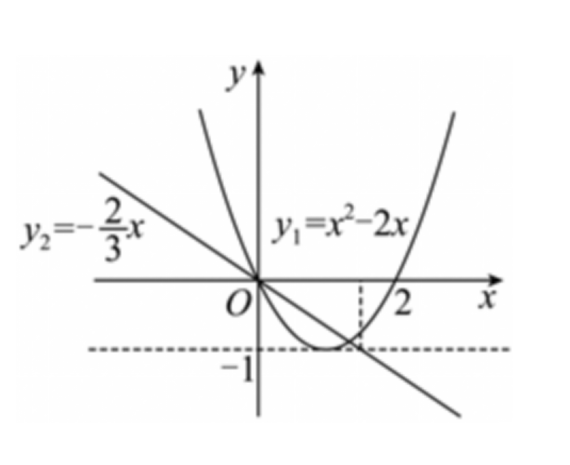
\includegraphics[width=0.24\textwidth]{figures/gao102_q7.png}
\end{center}
\step{当 $m>\dfrac32$ 时，当 $x>m$ 时 $f(x)\in\left(-\infty,-\dfrac23m\right)$，当 $x\leqslant m$ 时 $f(x)\in[-1,+\infty)$，}
\step{显然 $-\dfrac23m<-1$，此时函数 $f(x)$ 的值域不为 $R$，不符合题意；}
\step{当 $m<0$ 时，当 $x>m$ 时，$f(x)\in\left(-\infty,-\dfrac23m\right)$，}
\step{当 $x\leqslant m$ 时，$f(x)\in[m^2-2m,+\infty)$，}
\step{此时 $m^2-2m-\left(-\dfrac23m\right)=m^2-\dfrac43m=m\left(m-\dfrac43\right)>0$，即 $m^2-2m>-\dfrac23m$，}
\step{此时函数 $f(x)$ 的值域不为 $R$，不符合题意；}
\step{当 $0\leqslant m\leqslant\dfrac43$ 时，在 $x\in(0,m)$ 时 $y_2>y_1$，即 $m^2-2m<-\dfrac23m$，}
\step{此时 $f(x)$ 的值域为 $R$，符合题意，}
\step{当 $\dfrac43<m\leqslant\dfrac32$ 时，当 $x>m$ 时，$f(x)\in\left(-\infty,-\dfrac23m\right)$，}
\step{当 $x\leqslant m$ 时，$f(x)\in[-1,+\infty)$，}
\step{此时 $-1-\left(-\dfrac23m\right)=\dfrac23m-1\leqslant0$，即 $-1\leqslant-\dfrac23m$，}
\step{此时函数 $f(x)$ 的值域为 $R$，符合题意；}
\step{综上，$0\leqslant m\leqslant\dfrac32$，即实数 $m$ 的取值范围是 $\left[0,\dfrac32\right]$.}
\solend

\fi

\item 已知函数 $f(x)=x^2-2ax+b$（$a>1$）的定义域和值域都为 $[1,a]$，则 $b=$\blankline[4.4em].

\ifanswer
\solbegin
\step{$f(x)=x^2-2ax+b$（$a>1$）在 $[1,a]$ 严格减，}
\step{则 $f(1)=1-2a+b=a,f(a)=-a^2+b=1$，解得 $a=2,b=5$，所以 $b=5$.}
\solend

\fi

\item 若 $f(x)$ 满足 $f(x+y)=f(x)f(y)$，当 $x>0$ 时，$f(x)$ 的值域为 $(1,+\infty)$，则 $x<0$ 时，
$f(x)$ 的取值范围为\blankline[4.4em].

\ifanswer
\solbegin
\step{因为 $f(x+y)=f(x)f(y)$，令 $x=1$，$y=0$，得 $f(1+0)=f(1)f(0)$，}
\step{又因为当 $x>0$ 时，$f(x)>1$，所以 $f(1)>1>0$，故 $f(0)=1$.}
\step{当 $x<0$ 时，$-x>0$，令 $y=-x$，得 $f(x-x)=f(0)=1=f(x)f(-x)$，}
\step{故 $f(x)=\dfrac1{f(-x)}\in(0,1)$，故 $x<0$ 时，$f(x)$ 的取值范围为 $(0,1)$.}
\solend

\fi

\item 设函数 $f(x)=\begin{cases}x^2+x, & x<0\\ -x^2, & x\geqslant0\end{cases}$，若 $f(f(a))\leqslant2$，则实数 $a$ 的取值范围是\blankline[4.4em].

\ifanswer
\solbegin
\step{函数 $f(x)=\begin{cases}x^2+x, & x<0\\ -x^2, & x\geqslant0\end{cases}$，它的图象如图所示：}
\begin{center}
% 原图第 4 页解析插图直接裁取（原卷排于解析行右侧）。
% 裁框取图形区域，已去粉色水印转灰度。
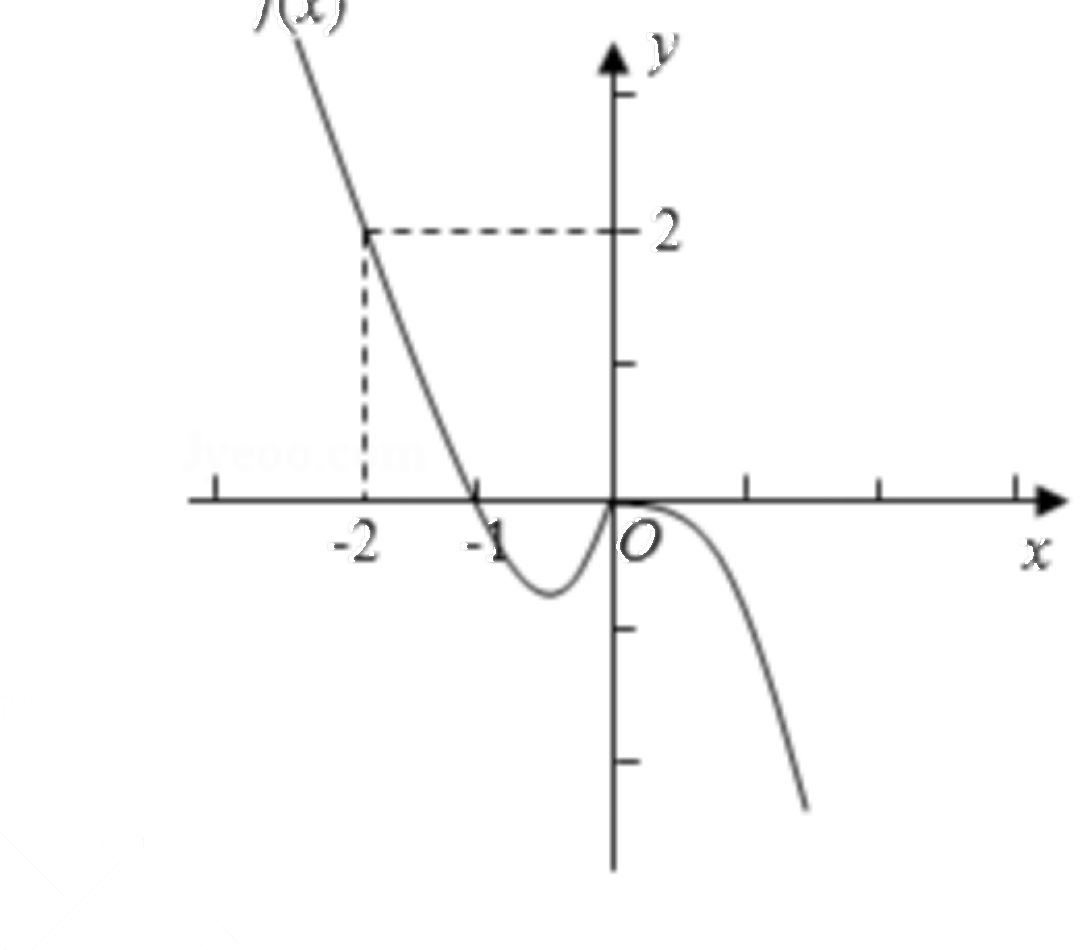
\includegraphics[width=0.30\textwidth]{figures/gao102_q10.png}
\end{center}
\step{由 $f(f(a))\leqslant2$，得 $f(a)\geqslant-2$.}
\step{当 $a<0$ 时，$f(a)=a^2+a=\left(a+\dfrac12\right)^2-\dfrac14\geqslant-2$ 恒成立；}
\step{当 $a\geqslant0$ 时，$f(a)=-a^2\geqslant-2$，即 $a^2\leqslant2$，解得 $0\leqslant a\leqslant\sqrt2$，}
\step{则实数 $a$ 的取值范围是 $(-\infty,\sqrt2]$.}
\solend

\fi

\item 已知二次函数 $f(x)$、$g(x)$ 的二次项系数均为 1，且满足
$\dfrac{f(2025)}{g(2025)}=\dfrac{f(2026)}{g(2026)}=\dfrac{2026}{2025}$，
则 $2026g(2027)-2025f(2027)$ 的值为\blankline[4.4em].

\ifanswer
\solbegin
\step{令 $h(x)=2026g(x)-2025f(x)$，其二次项系数为 $2026-2025=1$.}
\step{由比例条件得 $h(2025)=h(2026)=0$，}
\step{因此 $h(x)=(x-2025)(x-2026),h(2027)=2\times1=2$.}
\solend

\fi

\item 已知函数 $f(x)=\left\lvert x+\dfrac1x-a\right\rvert+1$，对任意实数 $x_1$、$x_2$、$x_3\in\left[\dfrac13,3\right]$，使得以
$f(x_1)$、$f(x_2)$、$f(x_3)$ 数值为边长可构成三角形，则实数 $a$ 的取值范围为\blankline[4.4em].

\ifanswer
\solbegin
\step{对任意实数 $x_1,x_2,x_3\in\left[\dfrac13,3\right]$，}
\step{使得以 $f(x_1)$、$f(x_2)$、$f(x_3)$ 数值为边长可构成三角形，}
\step{只需 $2f(x)_{\min}>f(x)_{\max}$，设 $g(x)=x+\dfrac1x-a$，}
\step{当 $x\in\left[\dfrac13,1\right)$ 时，函数 $g(x)$ 严格减，当 $x\in(1,3]$ 时，函数 $g(x)$ 严格增，}
\step{因为 $g(1)=2-a,g(3)=\dfrac{10}3-a,g\left(\dfrac13\right)=\dfrac{10}3-a$，所以 $g(x)\in\left[2-a,\dfrac{10}3-a\right]$，}
\step{当 $2-a\geqslant0$ 时，即 $a\leqslant2$ 时，$f(x)=\left\lvert x+\dfrac1x-a\right\rvert+1=g(x)+1$，}
\step{此时 $f(x)\in\left[3-a,\dfrac{13}3-a\right]$，}
\step{因此由 $2f(x)_{\min}>f(x)_{\max}\Rightarrow2(3-a)>\dfrac{13}3-a\Rightarrow a<\dfrac53$，而 $a\leqslant2$，所以 $a<\dfrac53$；}
\step{当 $\dfrac{10}3-a\leqslant0$，即 $a\geqslant\dfrac{10}3$ 时，$f(x)=\left\lvert x+\dfrac1x-a\right\rvert+1=-g(x)+1$，}
\step{此时 $f(x)\in\left[a-\dfrac73,a-1\right]$，}
\step{因此由 $2f(x)_{\min}>f(x)_{\max}\Rightarrow2\left(a-\dfrac73\right)>a-1\Rightarrow a>\dfrac{11}3$，而 $a\geqslant\dfrac{10}3$，所以 $a>\dfrac{11}3$，}
\step{若 $2-a<0<\dfrac{10}3-a$ 时，即 $2<a<\dfrac{10}3$ 时，}
\step{若 $a-2\geqslant\dfrac{10}3-a\Rightarrow a\geqslant\dfrac83$，即当 $\dfrac83\leqslant a<\dfrac{10}3$ 时，}
\step{显然此时 $f(x)_{\min}=1$，$f(x)_{\max}=a-2+1=a-1$，}
\step{由 $2f(x)_{\min}>f(x)_{\max}\Rightarrow2\times1>a-1\Rightarrow a<3$，显然 $\dfrac83\leqslant a<3$，}
\step{若 $a-2<\dfrac{10}3-a\Rightarrow a<\dfrac83$，即当 $2<a<\dfrac83$ 时，}
\step{显然此时 $f(x)_{\min}=1,f(x)_{\max}=\dfrac{10}3-a+1=\dfrac{13}3-a$，}
\step{因此由 $2f(x)_{\min}>f(x)_{\max}\Rightarrow2\times1>\dfrac{13}3-a\Rightarrow a>\dfrac73$，而 $\dfrac73<a<\dfrac83$，}
\step{综上，实数 $a$ 的取值范围为 $\left(-\infty,\dfrac53\right)\cup\left(\dfrac73,3\right)\cup\left(\dfrac{11}3,+\infty\right)$.}
\solend

\fi

\end{enumerate}

\bigsec{二、选择题}

\begin{enumerate}
\setcounter{enumi}{12}

\item 已知 $f(x)$ 是定义在 $\R$ 上的奇函数，$g(x)$ 是定义在 $\R$ 上的偶函数，则\mbox{（\quad）}

\keepwithprev
A. $f(x)g(x)$ 是偶函数\qquad B. $f(g(x))$ 是奇函数

C. $f(x)-g(x)$ 是奇函数\qquad D. $g(f(x))$ 是偶函数

\ifanswer
\solbegin
\step{$g(f(x))$ 的定义域为 $\R$，且 $g(f(-x))=g(-f(x))=g(f(x))$，}
\step{所以 $g(f(x))$ 是偶函数，故选 $D$.}
\solend

\fi

\item 已知定义在 $R$ 上的偶函数 $f(x)=\lvert x-m+1\rvert-2$，若正实数 $a$、$b$ 满足 $f(a)+f(2b)=m$，
则 $\dfrac1a+\dfrac2b$ 的最小值为\mbox{（\quad）}

\keepwithprev
A. $\dfrac95$\qquad\qquad B. $9$\qquad\qquad C. $\dfrac85$\qquad\qquad D. $8$

\ifanswer
\solbegin
\step{因为 $f(x)=\lvert x-m+1\rvert-2$ 是偶函数，所以 $-m+1=0$，所以 $m=1$，}
\step{所以 $f(x)=\lvert x\rvert-2$，若正实数 $a$、$b$ 满足 $f(a)+f(2b)=m$，}
\step{则 $a-2+2b-2=1$，所以 $a+2b=5$，}
\step{所以 $\dfrac1a+\dfrac2b=\dfrac15(a+2b)\left(\dfrac1a+\dfrac2b\right)=\dfrac15\left(5+\dfrac{2a}b+\dfrac{2b}a\right)\geqslant\dfrac95$，}
\step{当且仅当 $a=b=\dfrac53$ 时取等号，则 $\dfrac1a+\dfrac2b$ 的最小值为 $\dfrac95$，故选 $A$.}
\solend

\fi

\item 设函数 $g(x)=x^2-2$（$x\in\R$），$f(x)=\begin{cases}g(x)+x+4, & x<g(x)\\ g(x)-x, & x\geqslant g(x)\end{cases}$，则 $f(x)$ 的值域是

\mbox{（\quad）}

\keepwithprev
A. $\left[-\dfrac94,0\right]\cup(1,+\infty)$\qquad\qquad B. $[0,+\infty)$

C. $\left[-\dfrac94,+\infty\right)$\qquad\qquad D. $\left[-\dfrac94,0\right]\cup(2,+\infty)$

\ifanswer
\solbegin
\step{当 $x<g(x)$，即 $x<x^2-2$，$(x-2)(x+1)>0$ 时，$x>2$ 或 $x<-1$，}
\step{$f(x)=g(x)+x+4=x^2-2+x+4=x^2+x+2=(x+0.5)^2+1.75$，}
\step{其最小值趋向于 $f(-1)$ 即 2，无最大值，}
\step{因此这个区间的值域为 $(2,+\infty)$.}
\step{当 $x\geqslant g(x)$ 时，$-1\leqslant x\leqslant2$，$f(x)=g(x)-x=x^2-2-x=(x-0.5)^2-2.25$，}
\step{其最小值为 $f(0.5)=-2.25$，其最大值为 $f(2)=0$，}
\step{因此这区间的值域为 $[-2.25,0]$.}
\step{综上，函数值域为 $\left[-\dfrac94,0\right]\cup(2,+\infty)$，故选 $D$.}
\solend

\fi

\item 设 $D$ 是含数 1 的有限实数集，$f(x)$ 是定义在 $D$ 上的函数，若 $f(x)$ 的图象绕原点逆时针
旋转 $\dfrac{\pi}{6}$ 与原图象重合，则在以下各项中，$f(1)$ 的可能取值只能是\mbox{（\quad）}

\keepwithprev
A. $\sqrt3$\qquad\qquad B. $\dfrac{\sqrt3}2$\qquad\qquad C. $\dfrac{\sqrt3}3$\qquad\qquad D. $0$

\ifanswer
\solbegin
\step{问题相当于圆上由 12 个点为一组，每次绕原点逆时针旋转 $\dfrac{\pi}{6}$ 个单位后与下一个点}
\step{会重合。我们可以通过代入和赋值的方法，当 $f(1)=\sqrt3$、$\dfrac{\sqrt3}3$、$0$ 时，}
\step{此时得到的圆心角为 $\dfrac{\pi}{3}$、$\dfrac{\pi}{6}$、$0$，然而此时 $x=0$ 或者 $x=1$ 时，}
\step{都有 2 个 $y$ 与之对应，而我们知道函数的定义就是要求一个 $x$ 只能对应一个 $y$，}
\step{因此只有当 $x=\dfrac{\sqrt3}2$，此时旋转 $\dfrac{\pi}{6}$，此时满足一个 $x$ 只会对应一个 $y$，故选 $B$.}
\solend

\fi

\end{enumerate}

\bigsec{三、解答题}

\begin{enumerate}
\setcounter{enumi}{16}

\item 求下列函数的值域.

（1）$y=\dfrac{2x^2-3x+5}{x-1}\left(x\in\left[\dfrac32,3\right]\right)$；

（2）$f(x)=\sqrt{x}-\sqrt{2-x}+\sqrt{x(2-x)}$.

\ansspace*[10]

\ifanswer
\solbegin
\stepm{（1）}{令 $t=x-1$，则 $t\in\left[\dfrac12,2\right]$，原函数化为 $Y(t)=2t+\dfrac4t+1$.}
\step{当 $0<u<v$ 时，$Y(v)-Y(u)=2(v-u)\left(1-\dfrac2{uv}\right)$，}
\step{所以 $Y$ 在 $\left[\dfrac12,\sqrt2\right]$ 上严格递减，在 $[\sqrt2,2]$ 上严格递增.}
\step{由 $Y(\sqrt2)=4\sqrt2+1,Y\left(\dfrac12\right)=10,Y(2)=7$，得值域为 $[4\sqrt2+1,10]$.}
\stepm{（2）}{定义域为 $[0,2]$.}
\step{令 $s=\sqrt{x}-\sqrt{2-x}$，$\sqrt{x}$ 与 $-\sqrt{2-x}$ 均随 $x$ 严格递增，}
\step{$s$ 从 $-\sqrt2$ 递增到 $\sqrt2$，即 $s\in[-\sqrt2,\sqrt2]$.}
\step{由 $s^2=2-2\sqrt{x(2-x)}$，得 $f(x)=s+\dfrac{2-s^2}2=-\dfrac12(s-1)^2+\dfrac32$.}
\step{当 $s=1$ 时取得最大值 $\dfrac32$；当 $s=-\sqrt2$ 时取得最小值 $-\sqrt2$；}
\step{因此值域为 $\left[-\sqrt2,\dfrac32\right]$.}
\solend

\fi

\item 已知 $f(2x+1)=\dfrac{2x+1}{x+1}$.

（1）解不等式 $f(x)<x$；

（2）求 $f(1)+f(2)+\cdots+f(6)+f\left(\dfrac12\right)+f\left(\dfrac13\right)+\cdots+f\left(\dfrac16\right)$ 的值.

\ansspace*[12]

\ifanswer
\solbegin
\step{令 $t=2x+1$，则 $x=\dfrac{t-1}2$，得 $f(t)=\dfrac{2t}{t+1},t\neq-1$.}
\stepm{（1）}{不等式等价于 $\dfrac{2x}{x+1}<x\Leftrightarrow\dfrac{x(x-1)}{x+1}>0$.}
\step{以 $-1,0,1$ 分区间判断符号，得解集为 $(-1,0)\cup(1,+\infty)$.}
\stepm{（2）}{当 $x>0$ 时，$f(x)+f\left(\dfrac1x\right)=\dfrac{2x}{x+1}+\dfrac2{x+1}=2$.}
\step{将 $f(2),\cdots,f(6)$ 分别与其倒数对应的函数值配对，共 5 对，且 $f(1)=1$，}
\step{因此原式$=1+5\times2=11$.}
\solend

\fi

\item 已知函数 $f(x)$、$g(x)$ 是定义在 $R$ 上的函数，其中 $f(x)$ 是奇函数，$g(x)$ 是偶函数，且
$f(x)+g(x)=ax^2-x$.

（1）求 $f(x)$ 和 $g(x)$ 的解析式；

（2）$h(x)=f(x)+g(x)+(1-a)x^2-2ax+4$ 在 $[1,3]$ 上有两个零点，求实数 $a$ 的取值范
围.

\ansspace*[14]

\ifanswer
\solbegin
\stepm{（1）}{因为 $f(x)+g(x)=ax^2-x$①，所以 $f(-x)+g(-x)=ax^2+x$，}
\step{又 $f(x)$ 是奇函数，$g(x)$ 是偶函数，}
\step{所以 $f(-x)=-f(x)$，$g(-x)=g(x)$，}
\step{所以 $-f(x)+g(x)=ax^2+x$②，}
\step{联立①②解得 $f(x)=-x$，$g(x)=ax^2$.}
\stepm{（2）}{$h(x)=f(x)+g(x)+(1-a)x^2-2ax+4$}
\step{$=ax^2-x+(1-a)x^2-2ax+4=x^2-(2a+1)x+4$，}
\step{是开口向上，对称轴为 $x=\dfrac{2a+1}2$ 的二次函数，}
\step{因为 $h(x)$ 在 $[1,3]$ 上有两个零点，所以 $\begin{cases}\Delta=(2a+1)^2-16>0\\ 1<\dfrac{2a+1}2<3\\ h(1)=1-(2a+1)+4\geqslant0\\ h(3)=9-3(2a+1)+4\geqslant0\end{cases}$，}
\step{解得 $\dfrac32<a\leqslant\dfrac53$，故实数 $a$ 的取值范围为 $\left(\dfrac32,\dfrac53\right]$.}
\solend

\fi

\item 若函数 $f(x)$ 在区间 $[a,b]$ 上的值域恰为 $\left[\dfrac1b,\dfrac1a\right]$，则称区间 $[a,b]$ 为 $f(x)$ 的一个“倒域
区间”。已知定义在 $[-4,4]$ 上的奇函数 $g(x)$，当 $x\in[0,4]$ 时，$g(x)=-x^2+2x$.

（1）求 $g(x)$ 的解析式；

（2）若关于 $x$ 的方程 $g(x)=-mx-m$ 在 $(0,4)$ 上恰有两个不相等的实数根，求实数 $m$ 的
取值范围；

（3）求函数 $g(x)$ 在 $[-4,0]$ 内的“倒域区间”.

\ansspace*[16]

\ifanswer
\solbegin
\stepm{（1）}{当 $x\in[-4,0)$ 时，$-x\in(0,4]$，}
\step{由奇函数的定义得 $g(x)=-g(-x)=-[(-x)^2+2(-x)]=x^2+2x$，}
\step{所以 $g(x)=\begin{cases}-x^2+2x, & 0\leqslant x\leqslant4\\ x^2+2x, & -4\leqslant x<0\end{cases}$.}
\stepm{（2）}{方程 $g(x)=-mx-m$，即 $x^2-(m+2)x-m=0$，}
\step{设 $h(x)=x^2-(m+2)x-m$，$0<x<4$，}
\step{由题意得 $\begin{cases}h(0)=-m>0\\ h(4)=8-5m>0\\ \Delta=(m+2)^2+4m>0\\ 0<\dfrac{m+2}2<4\end{cases}$，解得 $2\sqrt3-4<m<0$，}
\step{即实数 $m$ 的取值范围是 $(2\sqrt3-4,0)$.}
\stepm{（3）}{易得当 $-4\leqslant a<b<0$ 时，$\dfrac1b<\dfrac1a$，}
\step{且 $g(x)$ 在 $[-4,-1]$ 上严格减，在 $[-1,0]$ 上严格增，}
\step{故当 $x\in[-4,0]$ 时，$g(x)_{\min}=g(-1)=-1$，}
\step{所以 $\dfrac1b\geqslant-1$，所以 $-4<b\leqslant-1$，所以 $-4\leqslant a<b\leqslant-1$，}
\step{则 $\begin{cases}g(a)=a^2+2a=\dfrac1a\\ g(b)=b^2+2b=\dfrac1b\\ -4\leqslant a<b\leqslant-1\end{cases}$，解得 $\begin{cases}a=-\dfrac{1+\sqrt5}2\\ b=-1\end{cases}$，}
\step{所以 $g(x)$ 在 $[-4,0]$ 内的“倒域区间”为 $\left[-\dfrac{1+\sqrt5}2,-1\right]$.}
\solend

\fi

\item 我们知道：函数 $y=f(x)$ 的图象关于坐标原点成中心对称图形的充要条件是函数
$y=f(x)$ 为奇函数。有同学发现可以推广为：函数 $y=f(x)$ 的图象关于点 $(a,b)$ 成中心对
称图形的充要条件为函数 $y=f(x+a)-b$ 为奇函数。已知函数 $f(x)=\dfrac{2x}{3-x}$.

（1）求函数 $f(x)$ 图象的对称中心；

（2）若定义在 $R$ 上的函数 $y=g(x)$ 的图象关于点 $(1,2)$ 对称，且 $g(1)=2$，当 $x\in[0,1)$
时，$g(x)=x^2-tx+t+1$.

（$i$）求 $g(-3)+g(5)$ 的值；

（$ii$）若对$\forall x_1\in[0,2]$，$\exists x_2\in[-3,2]$ 使得 $g(x_1)=f(x_2)$ 恒成立，求实数 $t$ 的取值范围.

\ansspace*[18]

\ifanswer
\solbegin
\stepm{（1）}{由 $f(x)=\dfrac{2x}{3-x}=-2+\dfrac6{3-x}$，}
\step{易得 $f(x+3)+2=-2+\dfrac6{3-(x+3)}+2=-\dfrac6x$ 为奇函数，}
\step{$f(x)$ 的图象关于 $(3,-2)$ 对称.}
\stepm{（2）}{（$i$）$y=g(x)$ 图象关于点 $(1,2)$ 对称，则 $g(1+x)+g(1-x)=4$，}
\step{令 $x=4$，则 $g(-3)+g(5)=4$.}
\step{（$ii$）有 $g(x)$ 在 $x\in[0,2]$ 的取值范围为 $f(x)$ 在 $x\in[-3,2]$ 的取值范围的}
\step{子集，}
\step{因为 $f(x)=\dfrac{2x}{3-x}=\dfrac{6-2(3-x)}{3-x}=\dfrac6{3-x}-2$ 在 $[-3,2]$ 上严格增，}
\step{所以 $f(x)$ 在 $x\in[-3,2]$ 上的取值范围为 $[-1,4]$，}
\step{记 $g(x)$ 的值域为 $A$，且 $g(1)=2$，当 $x\in[0,1)$ 时 $g(x)=x^2-tx+t+1$，}
\step{①当 $\dfrac t2\leqslant0$，即 $t\leqslant0$ 时，有 $g(x)$ 在 $[0,1)$ 上严格增，}
\step{由对称性得 $g(x)$ 在 $[1,2]$ 上严格增，故 $g(x)$ 在 $[0,2]$ 上严格增，}
\step{故 $g(x)_{\min}=g(0)=t+1$，$g(x)_{\max}=g(2)=4-(t+1)=3-t$，$t\leqslant0$，}
\step{则 $A=[t+1,3-t]\subseteq[-1,4]$，即 $\begin{cases}t\leqslant0\\ t+1\geqslant-1\\ 3-t\leqslant4\end{cases}$，解得 $-1\leqslant t\leqslant0$.}
\step{②当 $0<\dfrac t2<1$，即 $0<t<2$ 时，}
\step{$g(x)$ 在 $\left(0,\dfrac t2\right)$ 上严格减，在 $\left(\dfrac t2,1\right)$ 上严格增，}
\step{由对称性得 $g(x)$ 在 $\left(2-\dfrac t2,2\right)$ 上严格减，在 $\left(1,2-\dfrac t2\right)$ 上严格增，}
\step{故 $g(x)$ 在 $\left(0,\dfrac t2\right)$ 上严格减，在 $\left(\dfrac t2,2-\dfrac t2\right)$ 上严格增，}
\step{在 $\left(2-\dfrac t2,2\right)$ 上严格减，则 $A=\left[g\left(\dfrac t2\right),g\left(2-\dfrac t2\right)\right]$，}
\step{由 $0<t<2$，得 $g(0)=t+1\in(1,3)$，$g(2)=4-(t+1)=3-t\in(1,3)$，}
\step{$g\left(\dfrac t2\right)=-\dfrac{t^2}4+t+1=-\dfrac14(t-2)^2+2\in(1,2]$，}
\step{又 $g\left(\dfrac t2\right)+g\left(2-\dfrac t2\right)=4$，$g\left(2-\dfrac t2\right)\in(2,3)$，}
\step{当 $0<t<2$ 时，$A\subseteq[-1,4]$ 恒成立，}
\step{③当 $\dfrac t2\geqslant1$，即 $t\geqslant2$ 时，有 $g(x)$ 在 $[0,1)$ 上严格减，}
\step{由对称点 $(1,2)$ 得 $g(x)$ 在 $[1,2]$ 上严格减，所以 $g(x)$ 在 $[0,2]$ 上严格减，}
\step{故 $g(x)_{\max}=g(0)=t+1$，$g(x)_{\min}=g(2)=4-(t+1)=3-t$，$t\geqslant2$，}
\step{则 $A=[3-t,t+1]\subseteq[-1,4]$，即 $\begin{cases}t\geqslant2\\ t+1\leqslant4\\ 3-t\geqslant-1\end{cases}$，解得 $2\leqslant t\leqslant3$.}
\step{综上，$t$ 的范围为 $\{t\mid-1\leqslant t\leqslant3\}$.}
\solend

\fi

\end{enumerate}

\end{document}
"
%
% 原始材料：微信公众号“魔都数学加油站”文章，作者破晓，2026-11-01 21:56 发布；
% 连载“27学年高一102”，原文标题“27学年高一102——2026-2027年上海市华师大二附中高一上周末作业5函数”；
% 原文链接：https://mp.weixin.qq.com/s/CDvOCcxFskIe9aFUeKi3Ww。
% 正文为 13 张 PNG 页（第 1、2、10、13 页 2560×3620，其余 4762×6735），题目下印有【解析】，为讲评版。
% 题目、解析均据原图转录；卷面水印及公众号页脚未录入。
%
% 卷首标题：原卷印作“2026-2027 年华师大二附中高一上周末作业 5”（公众号标题中的“上海市”“函数”
% 卷面标题行没有，本稿照卷面），年份区间按全稿惯例排 en dash；原卷未印副标题，本稿按题目内容
% 标为“函数”（全稿首份以函数为单一模块的卷子）。
%
% 与原卷的排版差异：
%   ① 原文从第 3 题起，填空题编号为 3—12、选择题为 13—16、解答题为 17—21，本稿保留原题号；
%   ② 原卷每题下直接印【解析】，本稿按全稿惯例将解析置于答案版；选择题括号内未印答案，另由
%      解析末句“故选 X”给出；
%   ③ 原卷未印副标题，本稿按“知识模块”口径补出；
%   ④ 原卷填空横线按全稿惯例排为 \blankline[4.4em]；解答题按惯例加 \ansspace；选择题括号排
%      \mbox{（\quad）}、选项段前按惯例加 \keepwithprev；
%   ⑤ 原卷 $f(x)_{min}$、$f(x)_{max}$ 等下标排斜体，按 高一96 成例改正体 $\min$、$\max$；
%   ⑥ 原卷数集排斜体 $R$（第 13 题排粗体），按全稿惯例改 $\R$；
%   ⑦ 第 7、10 两题的解析插图裁自原图（去粉色水印转灰度），仅答案版显示。
%
% 原卷存疑／笔误（均照录加注）：
%   第 3 题解析“减去都对应 −2 和 2 的”措辞含糊（意为减去恒取 −2 与恒取 2 的两个常函数）；
%   第 15 题解析“其最小值趋向于 f(−1) 即 2”（该段 f(x)=x²+x+2 在 x→−1⁻ 时趋于 2、取不到）；
%   第 16 题解析末句“因此只有当 x=√3/2”（按上下文应为 f(1)=√3/2）；
%   第 16 题解析以 f(1)=√3、√3/3、0 赋值时称“得到的圆心角为 π/3、π/6、0”，其中 √3/3 对应
%   圆心角 π/6 的说法与该点 (1,√3/3) 的实际幅角一致，但与选项 C（√3/3）被排除的结论矛盾
%   （幅角 π/6 的点旋转 π/6 后落到幅角 π/3 处，仍占 12 等分点位，原卷解析未展开），照录。
%
% 行数核对：逐题数 \step/\stepm 条数，合计 155 条（Q3：2；Q4：3；Q5：6；Q6：5；Q7：19；
% Q8：2；Q9：4；Q10：5；Q11：3；Q12：19；Q13：2；Q14：5；Q15：8；Q16：5；Q17：10；
% Q18：6；Q19：10；Q20：13；Q21：28），与原卷印刷行逐题相等。
%
\documentclass[a4paper,11pt]{article}
\usepackage{common}

\begin{document}

\examtitlest[3]{2026--2027 年华师大二附中高一上周末作业 5}{函数}

\bigsec{一、填空题}

\begin{enumerate}
\setcounter{enumi}{2}

\item 已知函数 $y=f(x)$ 的定义域为 $\{-2,-1,1,2\}$，值域为 $\{-2,2\}$，则满足条件的函数
$y=f(x)$ 最多有\blankline[4.4em]个.

\ifanswer
\solbegin
\step{定义域中 4 个元素每个都可以对应 $-2$ 和 $2$ 中的一个，减去都对应 $-2$ 和 $2$ 的，}
\step{则满足条件的函数 $y=f(x)$ 最多有 $2^4-2=14$.}
\solend

\fi

\item 已知函数 $f(2x)$ 的定义域为 $[-2,2]$，则函数 $f(x-3)$ 的定义域为\blankline[4.4em].

\ifanswer
\solbegin
\step{因为函数 $f(2x)$ 的定义域为 $[-2,2]$，即 $-2\leqslant x\leqslant2$，所以 $-4\leqslant2x\leqslant4$，}
\step{得 $f(x)$ 的定义域为 $[-4,4]$，由 $-4\leqslant x-3\leqslant4$，解得 $-1\leqslant x\leqslant7$，}
\step{即函数 $f(x-3)$ 的定义域为 $[-1,7]$.}
\solend

\fi

\item 函数 $f(x)=\begin{cases}-x-1, & x<0\\ -x+1, & x>0\end{cases}$，则 $f(x)-f(-x)>1$ 的解集为\blankline[4.4em].

\ifanswer
\solbegin
\step{定义域为 $\{x\mid x\neq0\}$.}
\step{当 $x<0$ 时，$-x>0,f(-x)=x+1$，}
\step{$f(x)-f(-x)=(-x-1)-(x+1)=-2x-2>1$，得 $x<-\dfrac32$.}
\step{当 $x>0$ 时，$f(-x)=x-1,f(x)-f(-x)=(-x+1)-(x-1)=-2x+2>1$，}
\step{得 $0<x<\dfrac12$.}
\step{故解集为 $\left(-\infty,-\dfrac32\right)\cup\left(0,\dfrac12\right)$.}
\solend

\fi

\item 已知函数 $f(x)=x^2-2(m-3)x+5$ 在区间 $[2,+\infty)$ 上的最小值为 1，则实数 $m=$\blankline[4.4em].

\ifanswer
\solbegin
\step{函数 $f(x)$ 图象的对称轴为 $x=m-3$.}
\step{当 $m-3\leqslant2$，即 $m\leqslant5$ 时，$f(x)_{\min}=f(2)=9-4m+12=1$，解得 $m=5$；}
\step{当 $m-3>2$，即 $m>5$ 时，$f(x)_{\min}=f(m-3)=-m^2+6m-4=1$，}
\step{解得 $m=5$（舍去）或 $1$（舍去），}
\step{综上，$m=5$.}
\solend

\fi

\item 已知函数 $f(x)=\begin{cases}x^2-2x, & x\leqslant m\\ -\dfrac23x, & x>m\end{cases}$ 的值域为 $R$，则实数 $m$ 的取值范围是\blankline[4.4em].

\ifanswer
\solbegin
\step{对于函数 $y_1=x^2-2x$，则 $y_1=(x-1)^2-1\geqslant-1$，当且仅当 $x=1$ 时取等号，}
\step{且函数在 $(-\infty,1)$ 上严格减，在 $(1,+\infty)$ 上严格增，}
\step{对于函数 $y_2=-\dfrac23x$，令 $y_2=-1$，则 $x=\dfrac32$，且函数在定义域上严格减，}
\step{令 $x^2-2x=-\dfrac23x$，解得 $x=0$ 或 $x=\dfrac43$，}
\step{所以 $y_2=-\dfrac23x$ 与 $y_1=x^2-2x$ 的两个交点分别为 $(0,0)$、$\left(\dfrac43,-\dfrac89\right)$，}
\step{则函数 $y_2=-\dfrac23x$ 与 $y_1=x^2-2x$ 的图象如图所示：}
\begin{center}
% 原图第 2 页解析插图直接裁取（原卷排于解析行右侧）。
% 裁框取图形区域，已去粉色水印转灰度。
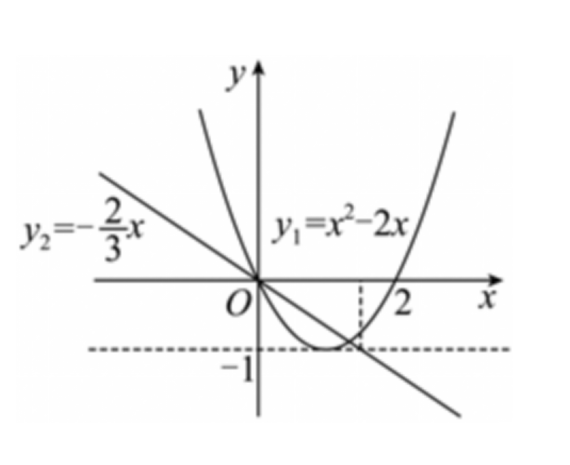
\includegraphics[width=0.24\textwidth]{figures/gao102_q7.png}
\end{center}
\step{当 $m>\dfrac32$ 时，当 $x>m$ 时 $f(x)\in\left(-\infty,-\dfrac23m\right)$，当 $x\leqslant m$ 时 $f(x)\in[-1,+\infty)$，}
\step{显然 $-\dfrac23m<-1$，此时函数 $f(x)$ 的值域不为 $R$，不符合题意；}
\step{当 $m<0$ 时，当 $x>m$ 时，$f(x)\in\left(-\infty,-\dfrac23m\right)$，}
\step{当 $x\leqslant m$ 时，$f(x)\in[m^2-2m,+\infty)$，}
\step{此时 $m^2-2m-\left(-\dfrac23m\right)=m^2-\dfrac43m=m\left(m-\dfrac43\right)>0$，即 $m^2-2m>-\dfrac23m$，}
\step{此时函数 $f(x)$ 的值域不为 $R$，不符合题意；}
\step{当 $0\leqslant m\leqslant\dfrac43$ 时，在 $x\in(0,m)$ 时 $y_2>y_1$，即 $m^2-2m<-\dfrac23m$，}
\step{此时 $f(x)$ 的值域为 $R$，符合题意，}
\step{当 $\dfrac43<m\leqslant\dfrac32$ 时，当 $x>m$ 时，$f(x)\in\left(-\infty,-\dfrac23m\right)$，}
\step{当 $x\leqslant m$ 时，$f(x)\in[-1,+\infty)$，}
\step{此时 $-1-\left(-\dfrac23m\right)=\dfrac23m-1\leqslant0$，即 $-1\leqslant-\dfrac23m$，}
\step{此时函数 $f(x)$ 的值域为 $R$，符合题意；}
\step{综上，$0\leqslant m\leqslant\dfrac32$，即实数 $m$ 的取值范围是 $\left[0,\dfrac32\right]$.}
\solend

\fi

\item 已知函数 $f(x)=x^2-2ax+b$（$a>1$）的定义域和值域都为 $[1,a]$，则 $b=$\blankline[4.4em].

\ifanswer
\solbegin
\step{$f(x)=x^2-2ax+b$（$a>1$）在 $[1,a]$ 严格减，}
\step{则 $f(1)=1-2a+b=a,f(a)=-a^2+b=1$，解得 $a=2,b=5$，所以 $b=5$.}
\solend

\fi

\item 若 $f(x)$ 满足 $f(x+y)=f(x)f(y)$，当 $x>0$ 时，$f(x)$ 的值域为 $(1,+\infty)$，则 $x<0$ 时，
$f(x)$ 的取值范围为\blankline[4.4em].

\ifanswer
\solbegin
\step{因为 $f(x+y)=f(x)f(y)$，令 $x=1$，$y=0$，得 $f(1+0)=f(1)f(0)$，}
\step{又因为当 $x>0$ 时，$f(x)>1$，所以 $f(1)>1>0$，故 $f(0)=1$.}
\step{当 $x<0$ 时，$-x>0$，令 $y=-x$，得 $f(x-x)=f(0)=1=f(x)f(-x)$，}
\step{故 $f(x)=\dfrac1{f(-x)}\in(0,1)$，故 $x<0$ 时，$f(x)$ 的取值范围为 $(0,1)$.}
\solend

\fi

\item 设函数 $f(x)=\begin{cases}x^2+x, & x<0\\ -x^2, & x\geqslant0\end{cases}$，若 $f(f(a))\leqslant2$，则实数 $a$ 的取值范围是\blankline[4.4em].

\ifanswer
\solbegin
\step{函数 $f(x)=\begin{cases}x^2+x, & x<0\\ -x^2, & x\geqslant0\end{cases}$，它的图象如图所示：}
\begin{center}
% 原图第 4 页解析插图直接裁取（原卷排于解析行右侧）。
% 裁框取图形区域，已去粉色水印转灰度。
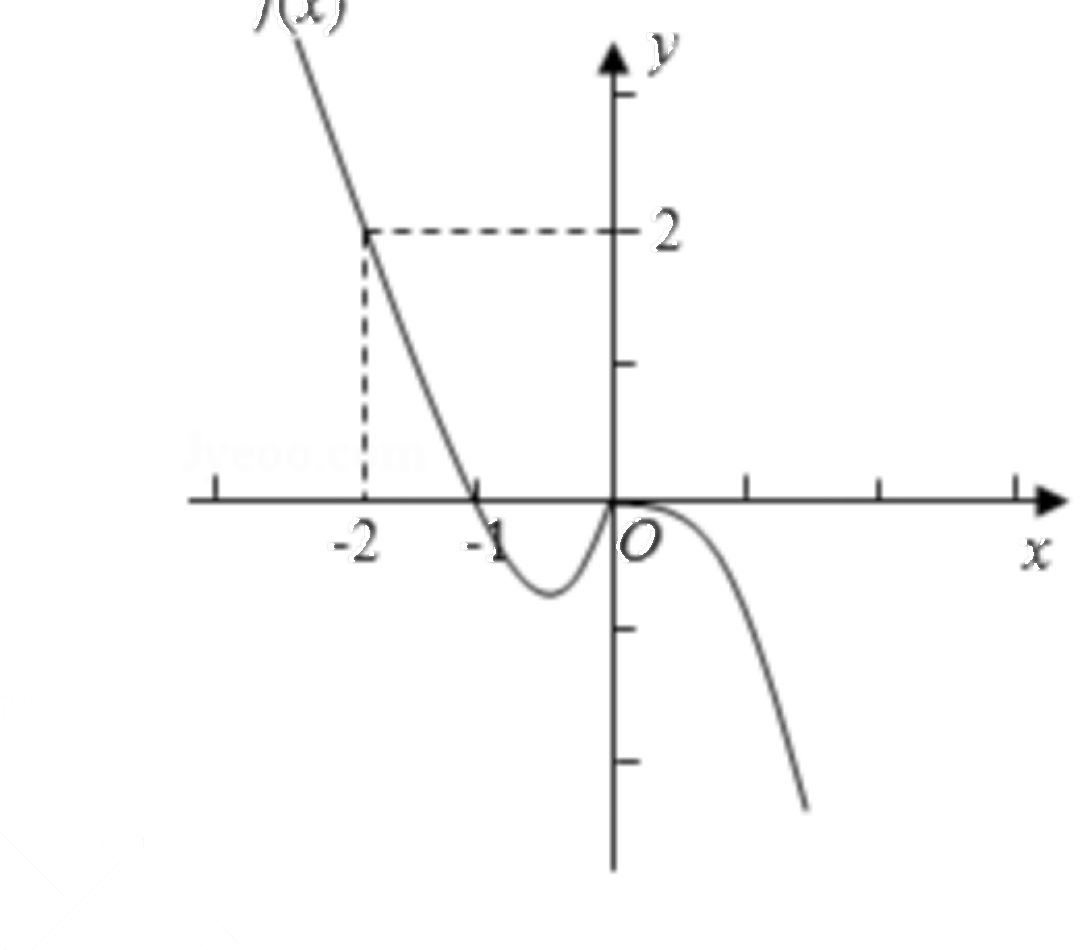
\includegraphics[width=0.30\textwidth]{figures/gao102_q10.png}
\end{center}
\step{由 $f(f(a))\leqslant2$，得 $f(a)\geqslant-2$.}
\step{当 $a<0$ 时，$f(a)=a^2+a=\left(a+\dfrac12\right)^2-\dfrac14\geqslant-2$ 恒成立；}
\step{当 $a\geqslant0$ 时，$f(a)=-a^2\geqslant-2$，即 $a^2\leqslant2$，解得 $0\leqslant a\leqslant\sqrt2$，}
\step{则实数 $a$ 的取值范围是 $(-\infty,\sqrt2]$.}
\solend

\fi

\item 已知二次函数 $f(x)$、$g(x)$ 的二次项系数均为 1，且满足
$\dfrac{f(2025)}{g(2025)}=\dfrac{f(2026)}{g(2026)}=\dfrac{2026}{2025}$，
则 $2026g(2027)-2025f(2027)$ 的值为\blankline[4.4em].

\ifanswer
\solbegin
\step{令 $h(x)=2026g(x)-2025f(x)$，其二次项系数为 $2026-2025=1$.}
\step{由比例条件得 $h(2025)=h(2026)=0$，}
\step{因此 $h(x)=(x-2025)(x-2026),h(2027)=2\times1=2$.}
\solend

\fi

\item 已知函数 $f(x)=\left\lvert x+\dfrac1x-a\right\rvert+1$，对任意实数 $x_1$、$x_2$、$x_3\in\left[\dfrac13,3\right]$，使得以
$f(x_1)$、$f(x_2)$、$f(x_3)$ 数值为边长可构成三角形，则实数 $a$ 的取值范围为\blankline[4.4em].

\ifanswer
\solbegin
\step{对任意实数 $x_1,x_2,x_3\in\left[\dfrac13,3\right]$，}
\step{使得以 $f(x_1)$、$f(x_2)$、$f(x_3)$ 数值为边长可构成三角形，}
\step{只需 $2f(x)_{\min}>f(x)_{\max}$，设 $g(x)=x+\dfrac1x-a$，}
\step{当 $x\in\left[\dfrac13,1\right)$ 时，函数 $g(x)$ 严格减，当 $x\in(1,3]$ 时，函数 $g(x)$ 严格增，}
\step{因为 $g(1)=2-a,g(3)=\dfrac{10}3-a,g\left(\dfrac13\right)=\dfrac{10}3-a$，所以 $g(x)\in\left[2-a,\dfrac{10}3-a\right]$，}
\step{当 $2-a\geqslant0$ 时，即 $a\leqslant2$ 时，$f(x)=\left\lvert x+\dfrac1x-a\right\rvert+1=g(x)+1$，}
\step{此时 $f(x)\in\left[3-a,\dfrac{13}3-a\right]$，}
\step{因此由 $2f(x)_{\min}>f(x)_{\max}\Rightarrow2(3-a)>\dfrac{13}3-a\Rightarrow a<\dfrac53$，而 $a\leqslant2$，所以 $a<\dfrac53$；}
\step{当 $\dfrac{10}3-a\leqslant0$，即 $a\geqslant\dfrac{10}3$ 时，$f(x)=\left\lvert x+\dfrac1x-a\right\rvert+1=-g(x)+1$，}
\step{此时 $f(x)\in\left[a-\dfrac73,a-1\right]$，}
\step{因此由 $2f(x)_{\min}>f(x)_{\max}\Rightarrow2\left(a-\dfrac73\right)>a-1\Rightarrow a>\dfrac{11}3$，而 $a\geqslant\dfrac{10}3$，所以 $a>\dfrac{11}3$，}
\step{若 $2-a<0<\dfrac{10}3-a$ 时，即 $2<a<\dfrac{10}3$ 时，}
\step{若 $a-2\geqslant\dfrac{10}3-a\Rightarrow a\geqslant\dfrac83$，即当 $\dfrac83\leqslant a<\dfrac{10}3$ 时，}
\step{显然此时 $f(x)_{\min}=1$，$f(x)_{\max}=a-2+1=a-1$，}
\step{由 $2f(x)_{\min}>f(x)_{\max}\Rightarrow2\times1>a-1\Rightarrow a<3$，显然 $\dfrac83\leqslant a<3$，}
\step{若 $a-2<\dfrac{10}3-a\Rightarrow a<\dfrac83$，即当 $2<a<\dfrac83$ 时，}
\step{显然此时 $f(x)_{\min}=1,f(x)_{\max}=\dfrac{10}3-a+1=\dfrac{13}3-a$，}
\step{因此由 $2f(x)_{\min}>f(x)_{\max}\Rightarrow2\times1>\dfrac{13}3-a\Rightarrow a>\dfrac73$，而 $\dfrac73<a<\dfrac83$，}
\step{综上，实数 $a$ 的取值范围为 $\left(-\infty,\dfrac53\right)\cup\left(\dfrac73,3\right)\cup\left(\dfrac{11}3,+\infty\right)$.}
\solend

\fi

\end{enumerate}

\bigsec{二、选择题}

\begin{enumerate}
\setcounter{enumi}{12}

\item 已知 $f(x)$ 是定义在 $\R$ 上的奇函数，$g(x)$ 是定义在 $\R$ 上的偶函数，则\mbox{（\quad）}

\keepwithprev
A. $f(x)g(x)$ 是偶函数\qquad B. $f(g(x))$ 是奇函数

C. $f(x)-g(x)$ 是奇函数\qquad D. $g(f(x))$ 是偶函数

\ifanswer
\solbegin
\step{$g(f(x))$ 的定义域为 $\R$，且 $g(f(-x))=g(-f(x))=g(f(x))$，}
\step{所以 $g(f(x))$ 是偶函数，故选 $D$.}
\solend

\fi

\item 已知定义在 $R$ 上的偶函数 $f(x)=\lvert x-m+1\rvert-2$，若正实数 $a$、$b$ 满足 $f(a)+f(2b)=m$，
则 $\dfrac1a+\dfrac2b$ 的最小值为\mbox{（\quad）}

\keepwithprev
A. $\dfrac95$\qquad\qquad B. $9$\qquad\qquad C. $\dfrac85$\qquad\qquad D. $8$

\ifanswer
\solbegin
\step{因为 $f(x)=\lvert x-m+1\rvert-2$ 是偶函数，所以 $-m+1=0$，所以 $m=1$，}
\step{所以 $f(x)=\lvert x\rvert-2$，若正实数 $a$、$b$ 满足 $f(a)+f(2b)=m$，}
\step{则 $a-2+2b-2=1$，所以 $a+2b=5$，}
\step{所以 $\dfrac1a+\dfrac2b=\dfrac15(a+2b)\left(\dfrac1a+\dfrac2b\right)=\dfrac15\left(5+\dfrac{2a}b+\dfrac{2b}a\right)\geqslant\dfrac95$，}
\step{当且仅当 $a=b=\dfrac53$ 时取等号，则 $\dfrac1a+\dfrac2b$ 的最小值为 $\dfrac95$，故选 $A$.}
\solend

\fi

\item 设函数 $g(x)=x^2-2$（$x\in\R$），$f(x)=\begin{cases}g(x)+x+4, & x<g(x)\\ g(x)-x, & x\geqslant g(x)\end{cases}$，则 $f(x)$ 的值域是

\mbox{（\quad）}

\keepwithprev
A. $\left[-\dfrac94,0\right]\cup(1,+\infty)$\qquad\qquad B. $[0,+\infty)$

C. $\left[-\dfrac94,+\infty\right)$\qquad\qquad D. $\left[-\dfrac94,0\right]\cup(2,+\infty)$

\ifanswer
\solbegin
\step{当 $x<g(x)$，即 $x<x^2-2$，$(x-2)(x+1)>0$ 时，$x>2$ 或 $x<-1$，}
\step{$f(x)=g(x)+x+4=x^2-2+x+4=x^2+x+2=(x+0.5)^2+1.75$，}
\step{其最小值趋向于 $f(-1)$ 即 2，无最大值，}
\step{因此这个区间的值域为 $(2,+\infty)$.}
\step{当 $x\geqslant g(x)$ 时，$-1\leqslant x\leqslant2$，$f(x)=g(x)-x=x^2-2-x=(x-0.5)^2-2.25$，}
\step{其最小值为 $f(0.5)=-2.25$，其最大值为 $f(2)=0$，}
\step{因此这区间的值域为 $[-2.25,0]$.}
\step{综上，函数值域为 $\left[-\dfrac94,0\right]\cup(2,+\infty)$，故选 $D$.}
\solend

\fi

\item 设 $D$ 是含数 1 的有限实数集，$f(x)$ 是定义在 $D$ 上的函数，若 $f(x)$ 的图象绕原点逆时针
旋转 $\dfrac{\pi}{6}$ 与原图象重合，则在以下各项中，$f(1)$ 的可能取值只能是\mbox{（\quad）}

\keepwithprev
A. $\sqrt3$\qquad\qquad B. $\dfrac{\sqrt3}2$\qquad\qquad C. $\dfrac{\sqrt3}3$\qquad\qquad D. $0$

\ifanswer
\solbegin
\step{问题相当于圆上由 12 个点为一组，每次绕原点逆时针旋转 $\dfrac{\pi}{6}$ 个单位后与下一个点}
\step{会重合。我们可以通过代入和赋值的方法，当 $f(1)=\sqrt3$、$\dfrac{\sqrt3}3$、$0$ 时，}
\step{此时得到的圆心角为 $\dfrac{\pi}{3}$、$\dfrac{\pi}{6}$、$0$，然而此时 $x=0$ 或者 $x=1$ 时，}
\step{都有 2 个 $y$ 与之对应，而我们知道函数的定义就是要求一个 $x$ 只能对应一个 $y$，}
\step{因此只有当 $x=\dfrac{\sqrt3}2$，此时旋转 $\dfrac{\pi}{6}$，此时满足一个 $x$ 只会对应一个 $y$，故选 $B$.}
\solend

\fi

\end{enumerate}

\bigsec{三、解答题}

\begin{enumerate}
\setcounter{enumi}{16}

\item 求下列函数的值域.

（1）$y=\dfrac{2x^2-3x+5}{x-1}\left(x\in\left[\dfrac32,3\right]\right)$；

（2）$f(x)=\sqrt{x}-\sqrt{2-x}+\sqrt{x(2-x)}$.

\ansspace*[10]

\ifanswer
\solbegin
\stepm{（1）}{令 $t=x-1$，则 $t\in\left[\dfrac12,2\right]$，原函数化为 $Y(t)=2t+\dfrac4t+1$.}
\step{当 $0<u<v$ 时，$Y(v)-Y(u)=2(v-u)\left(1-\dfrac2{uv}\right)$，}
\step{所以 $Y$ 在 $\left[\dfrac12,\sqrt2\right]$ 上严格递减，在 $[\sqrt2,2]$ 上严格递增.}
\step{由 $Y(\sqrt2)=4\sqrt2+1,Y\left(\dfrac12\right)=10,Y(2)=7$，得值域为 $[4\sqrt2+1,10]$.}
\stepm{（2）}{定义域为 $[0,2]$.}
\step{令 $s=\sqrt{x}-\sqrt{2-x}$，$\sqrt{x}$ 与 $-\sqrt{2-x}$ 均随 $x$ 严格递增，}
\step{$s$ 从 $-\sqrt2$ 递增到 $\sqrt2$，即 $s\in[-\sqrt2,\sqrt2]$.}
\step{由 $s^2=2-2\sqrt{x(2-x)}$，得 $f(x)=s+\dfrac{2-s^2}2=-\dfrac12(s-1)^2+\dfrac32$.}
\step{当 $s=1$ 时取得最大值 $\dfrac32$；当 $s=-\sqrt2$ 时取得最小值 $-\sqrt2$；}
\step{因此值域为 $\left[-\sqrt2,\dfrac32\right]$.}
\solend

\fi

\item 已知 $f(2x+1)=\dfrac{2x+1}{x+1}$.

（1）解不等式 $f(x)<x$；

（2）求 $f(1)+f(2)+\cdots+f(6)+f\left(\dfrac12\right)+f\left(\dfrac13\right)+\cdots+f\left(\dfrac16\right)$ 的值.

\ansspace*[12]

\ifanswer
\solbegin
\step{令 $t=2x+1$，则 $x=\dfrac{t-1}2$，得 $f(t)=\dfrac{2t}{t+1},t\neq-1$.}
\stepm{（1）}{不等式等价于 $\dfrac{2x}{x+1}<x\Leftrightarrow\dfrac{x(x-1)}{x+1}>0$.}
\step{以 $-1,0,1$ 分区间判断符号，得解集为 $(-1,0)\cup(1,+\infty)$.}
\stepm{（2）}{当 $x>0$ 时，$f(x)+f\left(\dfrac1x\right)=\dfrac{2x}{x+1}+\dfrac2{x+1}=2$.}
\step{将 $f(2),\cdots,f(6)$ 分别与其倒数对应的函数值配对，共 5 对，且 $f(1)=1$，}
\step{因此原式$=1+5\times2=11$.}
\solend

\fi

\item 已知函数 $f(x)$、$g(x)$ 是定义在 $R$ 上的函数，其中 $f(x)$ 是奇函数，$g(x)$ 是偶函数，且
$f(x)+g(x)=ax^2-x$.

（1）求 $f(x)$ 和 $g(x)$ 的解析式；

（2）$h(x)=f(x)+g(x)+(1-a)x^2-2ax+4$ 在 $[1,3]$ 上有两个零点，求实数 $a$ 的取值范
围.

\ansspace*[14]

\ifanswer
\solbegin
\stepm{（1）}{因为 $f(x)+g(x)=ax^2-x$①，所以 $f(-x)+g(-x)=ax^2+x$，}
\step{又 $f(x)$ 是奇函数，$g(x)$ 是偶函数，}
\step{所以 $f(-x)=-f(x)$，$g(-x)=g(x)$，}
\step{所以 $-f(x)+g(x)=ax^2+x$②，}
\step{联立①②解得 $f(x)=-x$，$g(x)=ax^2$.}
\stepm{（2）}{$h(x)=f(x)+g(x)+(1-a)x^2-2ax+4$}
\step{$=ax^2-x+(1-a)x^2-2ax+4=x^2-(2a+1)x+4$，}
\step{是开口向上，对称轴为 $x=\dfrac{2a+1}2$ 的二次函数，}
\step{因为 $h(x)$ 在 $[1,3]$ 上有两个零点，所以 $\begin{cases}\Delta=(2a+1)^2-16>0\\ 1<\dfrac{2a+1}2<3\\ h(1)=1-(2a+1)+4\geqslant0\\ h(3)=9-3(2a+1)+4\geqslant0\end{cases}$，}
\step{解得 $\dfrac32<a\leqslant\dfrac53$，故实数 $a$ 的取值范围为 $\left(\dfrac32,\dfrac53\right]$.}
\solend

\fi

\item 若函数 $f(x)$ 在区间 $[a,b]$ 上的值域恰为 $\left[\dfrac1b,\dfrac1a\right]$，则称区间 $[a,b]$ 为 $f(x)$ 的一个“倒域
区间”。已知定义在 $[-4,4]$ 上的奇函数 $g(x)$，当 $x\in[0,4]$ 时，$g(x)=-x^2+2x$.

（1）求 $g(x)$ 的解析式；

（2）若关于 $x$ 的方程 $g(x)=-mx-m$ 在 $(0,4)$ 上恰有两个不相等的实数根，求实数 $m$ 的
取值范围；

（3）求函数 $g(x)$ 在 $[-4,0]$ 内的“倒域区间”.

\ansspace*[16]

\ifanswer
\solbegin
\stepm{（1）}{当 $x\in[-4,0)$ 时，$-x\in(0,4]$，}
\step{由奇函数的定义得 $g(x)=-g(-x)=-[(-x)^2+2(-x)]=x^2+2x$，}
\step{所以 $g(x)=\begin{cases}-x^2+2x, & 0\leqslant x\leqslant4\\ x^2+2x, & -4\leqslant x<0\end{cases}$.}
\stepm{（2）}{方程 $g(x)=-mx-m$，即 $x^2-(m+2)x-m=0$，}
\step{设 $h(x)=x^2-(m+2)x-m$，$0<x<4$，}
\step{由题意得 $\begin{cases}h(0)=-m>0\\ h(4)=8-5m>0\\ \Delta=(m+2)^2+4m>0\\ 0<\dfrac{m+2}2<4\end{cases}$，解得 $2\sqrt3-4<m<0$，}
\step{即实数 $m$ 的取值范围是 $(2\sqrt3-4,0)$.}
\stepm{（3）}{易得当 $-4\leqslant a<b<0$ 时，$\dfrac1b<\dfrac1a$，}
\step{且 $g(x)$ 在 $[-4,-1]$ 上严格减，在 $[-1,0]$ 上严格增，}
\step{故当 $x\in[-4,0]$ 时，$g(x)_{\min}=g(-1)=-1$，}
\step{所以 $\dfrac1b\geqslant-1$，所以 $-4<b\leqslant-1$，所以 $-4\leqslant a<b\leqslant-1$，}
\step{则 $\begin{cases}g(a)=a^2+2a=\dfrac1a\\ g(b)=b^2+2b=\dfrac1b\\ -4\leqslant a<b\leqslant-1\end{cases}$，解得 $\begin{cases}a=-\dfrac{1+\sqrt5}2\\ b=-1\end{cases}$，}
\step{所以 $g(x)$ 在 $[-4,0]$ 内的“倒域区间”为 $\left[-\dfrac{1+\sqrt5}2,-1\right]$.}
\solend

\fi

\item 我们知道：函数 $y=f(x)$ 的图象关于坐标原点成中心对称图形的充要条件是函数
$y=f(x)$ 为奇函数。有同学发现可以推广为：函数 $y=f(x)$ 的图象关于点 $(a,b)$ 成中心对
称图形的充要条件为函数 $y=f(x+a)-b$ 为奇函数。已知函数 $f(x)=\dfrac{2x}{3-x}$.

（1）求函数 $f(x)$ 图象的对称中心；

（2）若定义在 $R$ 上的函数 $y=g(x)$ 的图象关于点 $(1,2)$ 对称，且 $g(1)=2$，当 $x\in[0,1)$
时，$g(x)=x^2-tx+t+1$.

（$i$）求 $g(-3)+g(5)$ 的值；

（$ii$）若对$\forall x_1\in[0,2]$，$\exists x_2\in[-3,2]$ 使得 $g(x_1)=f(x_2)$ 恒成立，求实数 $t$ 的取值范围.

\ansspace*[18]

\ifanswer
\solbegin
\stepm{（1）}{由 $f(x)=\dfrac{2x}{3-x}=-2+\dfrac6{3-x}$，}
\step{易得 $f(x+3)+2=-2+\dfrac6{3-(x+3)}+2=-\dfrac6x$ 为奇函数，}
\step{$f(x)$ 的图象关于 $(3,-2)$ 对称.}
\stepm{（2）}{（$i$）$y=g(x)$ 图象关于点 $(1,2)$ 对称，则 $g(1+x)+g(1-x)=4$，}
\step{令 $x=4$，则 $g(-3)+g(5)=4$.}
\step{（$ii$）有 $g(x)$ 在 $x\in[0,2]$ 的取值范围为 $f(x)$ 在 $x\in[-3,2]$ 的取值范围的}
\step{子集，}
\step{因为 $f(x)=\dfrac{2x}{3-x}=\dfrac{6-2(3-x)}{3-x}=\dfrac6{3-x}-2$ 在 $[-3,2]$ 上严格增，}
\step{所以 $f(x)$ 在 $x\in[-3,2]$ 上的取值范围为 $[-1,4]$，}
\step{记 $g(x)$ 的值域为 $A$，且 $g(1)=2$，当 $x\in[0,1)$ 时 $g(x)=x^2-tx+t+1$，}
\step{①当 $\dfrac t2\leqslant0$，即 $t\leqslant0$ 时，有 $g(x)$ 在 $[0,1)$ 上严格增，}
\step{由对称性得 $g(x)$ 在 $[1,2]$ 上严格增，故 $g(x)$ 在 $[0,2]$ 上严格增，}
\step{故 $g(x)_{\min}=g(0)=t+1$，$g(x)_{\max}=g(2)=4-(t+1)=3-t$，$t\leqslant0$，}
\step{则 $A=[t+1,3-t]\subseteq[-1,4]$，即 $\begin{cases}t\leqslant0\\ t+1\geqslant-1\\ 3-t\leqslant4\end{cases}$，解得 $-1\leqslant t\leqslant0$.}
\step{②当 $0<\dfrac t2<1$，即 $0<t<2$ 时，}
\step{$g(x)$ 在 $\left(0,\dfrac t2\right)$ 上严格减，在 $\left(\dfrac t2,1\right)$ 上严格增，}
\step{由对称性得 $g(x)$ 在 $\left(2-\dfrac t2,2\right)$ 上严格减，在 $\left(1,2-\dfrac t2\right)$ 上严格增，}
\step{故 $g(x)$ 在 $\left(0,\dfrac t2\right)$ 上严格减，在 $\left(\dfrac t2,2-\dfrac t2\right)$ 上严格增，}
\step{在 $\left(2-\dfrac t2,2\right)$ 上严格减，则 $A=\left[g\left(\dfrac t2\right),g\left(2-\dfrac t2\right)\right]$，}
\step{由 $0<t<2$，得 $g(0)=t+1\in(1,3)$，$g(2)=4-(t+1)=3-t\in(1,3)$，}
\step{$g\left(\dfrac t2\right)=-\dfrac{t^2}4+t+1=-\dfrac14(t-2)^2+2\in(1,2]$，}
\step{又 $g\left(\dfrac t2\right)+g\left(2-\dfrac t2\right)=4$，$g\left(2-\dfrac t2\right)\in(2,3)$，}
\step{当 $0<t<2$ 时，$A\subseteq[-1,4]$ 恒成立，}
\step{③当 $\dfrac t2\geqslant1$，即 $t\geqslant2$ 时，有 $g(x)$ 在 $[0,1)$ 上严格减，}
\step{由对称点 $(1,2)$ 得 $g(x)$ 在 $[1,2]$ 上严格减，所以 $g(x)$ 在 $[0,2]$ 上严格减，}
\step{故 $g(x)_{\max}=g(0)=t+1$，$g(x)_{\min}=g(2)=4-(t+1)=3-t$，$t\geqslant2$，}
\step{则 $A=[3-t,t+1]\subseteq[-1,4]$，即 $\begin{cases}t\geqslant2\\ t+1\leqslant4\\ 3-t\geqslant-1\end{cases}$，解得 $2\leqslant t\leqslant3$.}
\step{综上，$t$ 的范围为 $\{t\mid-1\leqslant t\leqslant3\}$.}
\solend

\fi

\end{enumerate}

\end{document}
"
% 紧凑版：xelatex "\def\iscompact{1}% 高一102_华师大二附中_周末作业5.tex
%   —— 高一上数学“2026-2027 年华师大二附中高一上周末作业 5”（试卷版/答案版）
% 试卷版：xelatex 高一102_华师大二附中_周末作业5.tex
% 答案版：xelatex "\def\isanswer{1}% 高一102_华师大二附中_周末作业5.tex
%   —— 高一上数学“2026-2027 年华师大二附中高一上周末作业 5”（试卷版/答案版）
% 试卷版：xelatex 高一102_华师大二附中_周末作业5.tex
% 答案版：xelatex "\def\isanswer{1}% 高一102_华师大二附中_周末作业5.tex
%   —— 高一上数学“2026-2027 年华师大二附中高一上周末作业 5”（试卷版/答案版）
% 试卷版：xelatex 高一102_华师大二附中_周末作业5.tex
% 答案版：xelatex "\def\isanswer{1}\input{高一102_华师大二附中_周末作业5.tex}"
% 紧凑版：xelatex "\def\iscompact{1}\input{高一102_华师大二附中_周末作业5.tex}"
%
% 原始材料：微信公众号“魔都数学加油站”文章，作者破晓，2026-11-01 21:56 发布；
% 连载“27学年高一102”，原文标题“27学年高一102——2026-2027年上海市华师大二附中高一上周末作业5函数”；
% 原文链接：https://mp.weixin.qq.com/s/CDvOCcxFskIe9aFUeKi3Ww。
% 正文为 13 张 PNG 页（第 1、2、10、13 页 2560×3620，其余 4762×6735），题目下印有【解析】，为讲评版。
% 题目、解析均据原图转录；卷面水印及公众号页脚未录入。
%
% 卷首标题：原卷印作“2026-2027 年华师大二附中高一上周末作业 5”（公众号标题中的“上海市”“函数”
% 卷面标题行没有，本稿照卷面），年份区间按全稿惯例排 en dash；原卷未印副标题，本稿按题目内容
% 标为“函数”（全稿首份以函数为单一模块的卷子）。
%
% 与原卷的排版差异：
%   ① 原文从第 3 题起，填空题编号为 3—12、选择题为 13—16、解答题为 17—21，本稿保留原题号；
%   ② 原卷每题下直接印【解析】，本稿按全稿惯例将解析置于答案版；选择题括号内未印答案，另由
%      解析末句“故选 X”给出；
%   ③ 原卷未印副标题，本稿按“知识模块”口径补出；
%   ④ 原卷填空横线按全稿惯例排为 \blankline[4.4em]；解答题按惯例加 \ansspace；选择题括号排
%      \mbox{（\quad）}、选项段前按惯例加 \keepwithprev；
%   ⑤ 原卷 $f(x)_{min}$、$f(x)_{max}$ 等下标排斜体，按 高一96 成例改正体 $\min$、$\max$；
%   ⑥ 原卷数集排斜体 $R$（第 13 题排粗体），按全稿惯例改 $\R$；
%   ⑦ 第 7、10 两题的解析插图裁自原图（去粉色水印转灰度），仅答案版显示。
%
% 原卷存疑／笔误（均照录加注）：
%   第 3 题解析“减去都对应 −2 和 2 的”措辞含糊（意为减去恒取 −2 与恒取 2 的两个常函数）；
%   第 15 题解析“其最小值趋向于 f(−1) 即 2”（该段 f(x)=x²+x+2 在 x→−1⁻ 时趋于 2、取不到）；
%   第 16 题解析末句“因此只有当 x=√3/2”（按上下文应为 f(1)=√3/2）；
%   第 16 题解析以 f(1)=√3、√3/3、0 赋值时称“得到的圆心角为 π/3、π/6、0”，其中 √3/3 对应
%   圆心角 π/6 的说法与该点 (1,√3/3) 的实际幅角一致，但与选项 C（√3/3）被排除的结论矛盾
%   （幅角 π/6 的点旋转 π/6 后落到幅角 π/3 处，仍占 12 等分点位，原卷解析未展开），照录。
%
% 行数核对：逐题数 \step/\stepm 条数，合计 155 条（Q3：2；Q4：3；Q5：6；Q6：5；Q7：19；
% Q8：2；Q9：4；Q10：5；Q11：3；Q12：19；Q13：2；Q14：5；Q15：8；Q16：5；Q17：10；
% Q18：6；Q19：10；Q20：13；Q21：28），与原卷印刷行逐题相等。
%
\documentclass[a4paper,11pt]{article}
\usepackage{common}

\begin{document}

\examtitlest[3]{2026--2027 年华师大二附中高一上周末作业 5}{函数}

\bigsec{一、填空题}

\begin{enumerate}
\setcounter{enumi}{2}

\item 已知函数 $y=f(x)$ 的定义域为 $\{-2,-1,1,2\}$，值域为 $\{-2,2\}$，则满足条件的函数
$y=f(x)$ 最多有\blankline[4.4em]个.

\ifanswer
\solbegin
\step{定义域中 4 个元素每个都可以对应 $-2$ 和 $2$ 中的一个，减去都对应 $-2$ 和 $2$ 的，}
\step{则满足条件的函数 $y=f(x)$ 最多有 $2^4-2=14$.}
\solend

\fi

\item 已知函数 $f(2x)$ 的定义域为 $[-2,2]$，则函数 $f(x-3)$ 的定义域为\blankline[4.4em].

\ifanswer
\solbegin
\step{因为函数 $f(2x)$ 的定义域为 $[-2,2]$，即 $-2\leqslant x\leqslant2$，所以 $-4\leqslant2x\leqslant4$，}
\step{得 $f(x)$ 的定义域为 $[-4,4]$，由 $-4\leqslant x-3\leqslant4$，解得 $-1\leqslant x\leqslant7$，}
\step{即函数 $f(x-3)$ 的定义域为 $[-1,7]$.}
\solend

\fi

\item 函数 $f(x)=\begin{cases}-x-1, & x<0\\ -x+1, & x>0\end{cases}$，则 $f(x)-f(-x)>1$ 的解集为\blankline[4.4em].

\ifanswer
\solbegin
\step{定义域为 $\{x\mid x\neq0\}$.}
\step{当 $x<0$ 时，$-x>0,f(-x)=x+1$，}
\step{$f(x)-f(-x)=(-x-1)-(x+1)=-2x-2>1$，得 $x<-\dfrac32$.}
\step{当 $x>0$ 时，$f(-x)=x-1,f(x)-f(-x)=(-x+1)-(x-1)=-2x+2>1$，}
\step{得 $0<x<\dfrac12$.}
\step{故解集为 $\left(-\infty,-\dfrac32\right)\cup\left(0,\dfrac12\right)$.}
\solend

\fi

\item 已知函数 $f(x)=x^2-2(m-3)x+5$ 在区间 $[2,+\infty)$ 上的最小值为 1，则实数 $m=$\blankline[4.4em].

\ifanswer
\solbegin
\step{函数 $f(x)$ 图象的对称轴为 $x=m-3$.}
\step{当 $m-3\leqslant2$，即 $m\leqslant5$ 时，$f(x)_{\min}=f(2)=9-4m+12=1$，解得 $m=5$；}
\step{当 $m-3>2$，即 $m>5$ 时，$f(x)_{\min}=f(m-3)=-m^2+6m-4=1$，}
\step{解得 $m=5$（舍去）或 $1$（舍去），}
\step{综上，$m=5$.}
\solend

\fi

\item 已知函数 $f(x)=\begin{cases}x^2-2x, & x\leqslant m\\ -\dfrac23x, & x>m\end{cases}$ 的值域为 $R$，则实数 $m$ 的取值范围是\blankline[4.4em].

\ifanswer
\solbegin
\step{对于函数 $y_1=x^2-2x$，则 $y_1=(x-1)^2-1\geqslant-1$，当且仅当 $x=1$ 时取等号，}
\step{且函数在 $(-\infty,1)$ 上严格减，在 $(1,+\infty)$ 上严格增，}
\step{对于函数 $y_2=-\dfrac23x$，令 $y_2=-1$，则 $x=\dfrac32$，且函数在定义域上严格减，}
\step{令 $x^2-2x=-\dfrac23x$，解得 $x=0$ 或 $x=\dfrac43$，}
\step{所以 $y_2=-\dfrac23x$ 与 $y_1=x^2-2x$ 的两个交点分别为 $(0,0)$、$\left(\dfrac43,-\dfrac89\right)$，}
\step{则函数 $y_2=-\dfrac23x$ 与 $y_1=x^2-2x$ 的图象如图所示：}
\begin{center}
% 原图第 2 页解析插图直接裁取（原卷排于解析行右侧）。
% 裁框取图形区域，已去粉色水印转灰度。
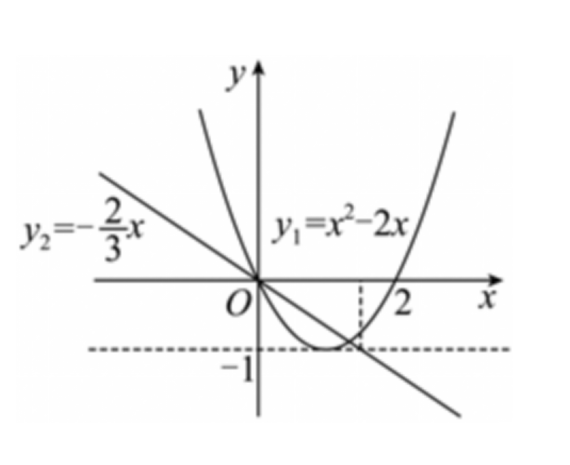
\includegraphics[width=0.24\textwidth]{figures/gao102_q7.png}
\end{center}
\step{当 $m>\dfrac32$ 时，当 $x>m$ 时 $f(x)\in\left(-\infty,-\dfrac23m\right)$，当 $x\leqslant m$ 时 $f(x)\in[-1,+\infty)$，}
\step{显然 $-\dfrac23m<-1$，此时函数 $f(x)$ 的值域不为 $R$，不符合题意；}
\step{当 $m<0$ 时，当 $x>m$ 时，$f(x)\in\left(-\infty,-\dfrac23m\right)$，}
\step{当 $x\leqslant m$ 时，$f(x)\in[m^2-2m,+\infty)$，}
\step{此时 $m^2-2m-\left(-\dfrac23m\right)=m^2-\dfrac43m=m\left(m-\dfrac43\right)>0$，即 $m^2-2m>-\dfrac23m$，}
\step{此时函数 $f(x)$ 的值域不为 $R$，不符合题意；}
\step{当 $0\leqslant m\leqslant\dfrac43$ 时，在 $x\in(0,m)$ 时 $y_2>y_1$，即 $m^2-2m<-\dfrac23m$，}
\step{此时 $f(x)$ 的值域为 $R$，符合题意，}
\step{当 $\dfrac43<m\leqslant\dfrac32$ 时，当 $x>m$ 时，$f(x)\in\left(-\infty,-\dfrac23m\right)$，}
\step{当 $x\leqslant m$ 时，$f(x)\in[-1,+\infty)$，}
\step{此时 $-1-\left(-\dfrac23m\right)=\dfrac23m-1\leqslant0$，即 $-1\leqslant-\dfrac23m$，}
\step{此时函数 $f(x)$ 的值域为 $R$，符合题意；}
\step{综上，$0\leqslant m\leqslant\dfrac32$，即实数 $m$ 的取值范围是 $\left[0,\dfrac32\right]$.}
\solend

\fi

\item 已知函数 $f(x)=x^2-2ax+b$（$a>1$）的定义域和值域都为 $[1,a]$，则 $b=$\blankline[4.4em].

\ifanswer
\solbegin
\step{$f(x)=x^2-2ax+b$（$a>1$）在 $[1,a]$ 严格减，}
\step{则 $f(1)=1-2a+b=a,f(a)=-a^2+b=1$，解得 $a=2,b=5$，所以 $b=5$.}
\solend

\fi

\item 若 $f(x)$ 满足 $f(x+y)=f(x)f(y)$，当 $x>0$ 时，$f(x)$ 的值域为 $(1,+\infty)$，则 $x<0$ 时，
$f(x)$ 的取值范围为\blankline[4.4em].

\ifanswer
\solbegin
\step{因为 $f(x+y)=f(x)f(y)$，令 $x=1$，$y=0$，得 $f(1+0)=f(1)f(0)$，}
\step{又因为当 $x>0$ 时，$f(x)>1$，所以 $f(1)>1>0$，故 $f(0)=1$.}
\step{当 $x<0$ 时，$-x>0$，令 $y=-x$，得 $f(x-x)=f(0)=1=f(x)f(-x)$，}
\step{故 $f(x)=\dfrac1{f(-x)}\in(0,1)$，故 $x<0$ 时，$f(x)$ 的取值范围为 $(0,1)$.}
\solend

\fi

\item 设函数 $f(x)=\begin{cases}x^2+x, & x<0\\ -x^2, & x\geqslant0\end{cases}$，若 $f(f(a))\leqslant2$，则实数 $a$ 的取值范围是\blankline[4.4em].

\ifanswer
\solbegin
\step{函数 $f(x)=\begin{cases}x^2+x, & x<0\\ -x^2, & x\geqslant0\end{cases}$，它的图象如图所示：}
\begin{center}
% 原图第 4 页解析插图直接裁取（原卷排于解析行右侧）。
% 裁框取图形区域，已去粉色水印转灰度。
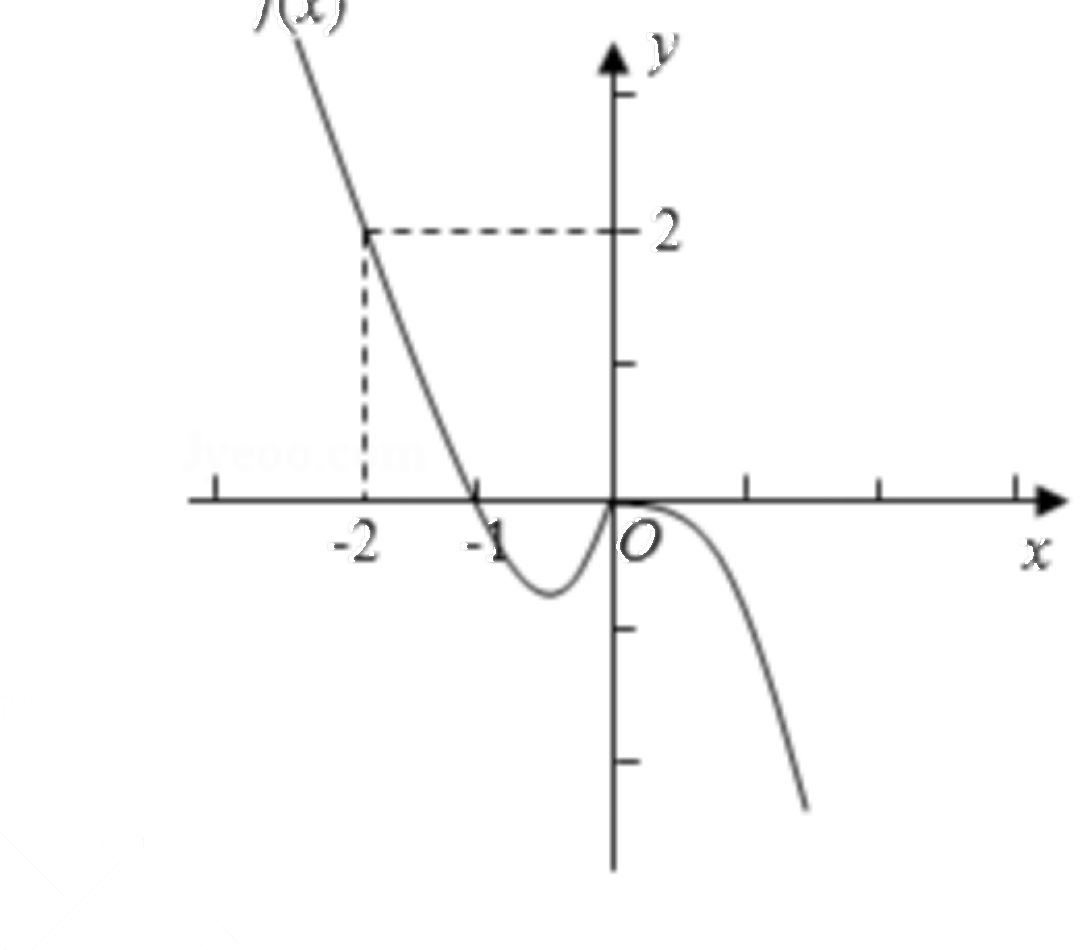
\includegraphics[width=0.30\textwidth]{figures/gao102_q10.png}
\end{center}
\step{由 $f(f(a))\leqslant2$，得 $f(a)\geqslant-2$.}
\step{当 $a<0$ 时，$f(a)=a^2+a=\left(a+\dfrac12\right)^2-\dfrac14\geqslant-2$ 恒成立；}
\step{当 $a\geqslant0$ 时，$f(a)=-a^2\geqslant-2$，即 $a^2\leqslant2$，解得 $0\leqslant a\leqslant\sqrt2$，}
\step{则实数 $a$ 的取值范围是 $(-\infty,\sqrt2]$.}
\solend

\fi

\item 已知二次函数 $f(x)$、$g(x)$ 的二次项系数均为 1，且满足
$\dfrac{f(2025)}{g(2025)}=\dfrac{f(2026)}{g(2026)}=\dfrac{2026}{2025}$，
则 $2026g(2027)-2025f(2027)$ 的值为\blankline[4.4em].

\ifanswer
\solbegin
\step{令 $h(x)=2026g(x)-2025f(x)$，其二次项系数为 $2026-2025=1$.}
\step{由比例条件得 $h(2025)=h(2026)=0$，}
\step{因此 $h(x)=(x-2025)(x-2026),h(2027)=2\times1=2$.}
\solend

\fi

\item 已知函数 $f(x)=\left\lvert x+\dfrac1x-a\right\rvert+1$，对任意实数 $x_1$、$x_2$、$x_3\in\left[\dfrac13,3\right]$，使得以
$f(x_1)$、$f(x_2)$、$f(x_3)$ 数值为边长可构成三角形，则实数 $a$ 的取值范围为\blankline[4.4em].

\ifanswer
\solbegin
\step{对任意实数 $x_1,x_2,x_3\in\left[\dfrac13,3\right]$，}
\step{使得以 $f(x_1)$、$f(x_2)$、$f(x_3)$ 数值为边长可构成三角形，}
\step{只需 $2f(x)_{\min}>f(x)_{\max}$，设 $g(x)=x+\dfrac1x-a$，}
\step{当 $x\in\left[\dfrac13,1\right)$ 时，函数 $g(x)$ 严格减，当 $x\in(1,3]$ 时，函数 $g(x)$ 严格增，}
\step{因为 $g(1)=2-a,g(3)=\dfrac{10}3-a,g\left(\dfrac13\right)=\dfrac{10}3-a$，所以 $g(x)\in\left[2-a,\dfrac{10}3-a\right]$，}
\step{当 $2-a\geqslant0$ 时，即 $a\leqslant2$ 时，$f(x)=\left\lvert x+\dfrac1x-a\right\rvert+1=g(x)+1$，}
\step{此时 $f(x)\in\left[3-a,\dfrac{13}3-a\right]$，}
\step{因此由 $2f(x)_{\min}>f(x)_{\max}\Rightarrow2(3-a)>\dfrac{13}3-a\Rightarrow a<\dfrac53$，而 $a\leqslant2$，所以 $a<\dfrac53$；}
\step{当 $\dfrac{10}3-a\leqslant0$，即 $a\geqslant\dfrac{10}3$ 时，$f(x)=\left\lvert x+\dfrac1x-a\right\rvert+1=-g(x)+1$，}
\step{此时 $f(x)\in\left[a-\dfrac73,a-1\right]$，}
\step{因此由 $2f(x)_{\min}>f(x)_{\max}\Rightarrow2\left(a-\dfrac73\right)>a-1\Rightarrow a>\dfrac{11}3$，而 $a\geqslant\dfrac{10}3$，所以 $a>\dfrac{11}3$，}
\step{若 $2-a<0<\dfrac{10}3-a$ 时，即 $2<a<\dfrac{10}3$ 时，}
\step{若 $a-2\geqslant\dfrac{10}3-a\Rightarrow a\geqslant\dfrac83$，即当 $\dfrac83\leqslant a<\dfrac{10}3$ 时，}
\step{显然此时 $f(x)_{\min}=1$，$f(x)_{\max}=a-2+1=a-1$，}
\step{由 $2f(x)_{\min}>f(x)_{\max}\Rightarrow2\times1>a-1\Rightarrow a<3$，显然 $\dfrac83\leqslant a<3$，}
\step{若 $a-2<\dfrac{10}3-a\Rightarrow a<\dfrac83$，即当 $2<a<\dfrac83$ 时，}
\step{显然此时 $f(x)_{\min}=1,f(x)_{\max}=\dfrac{10}3-a+1=\dfrac{13}3-a$，}
\step{因此由 $2f(x)_{\min}>f(x)_{\max}\Rightarrow2\times1>\dfrac{13}3-a\Rightarrow a>\dfrac73$，而 $\dfrac73<a<\dfrac83$，}
\step{综上，实数 $a$ 的取值范围为 $\left(-\infty,\dfrac53\right)\cup\left(\dfrac73,3\right)\cup\left(\dfrac{11}3,+\infty\right)$.}
\solend

\fi

\end{enumerate}

\bigsec{二、选择题}

\begin{enumerate}
\setcounter{enumi}{12}

\item 已知 $f(x)$ 是定义在 $\R$ 上的奇函数，$g(x)$ 是定义在 $\R$ 上的偶函数，则\mbox{（\quad）}

\keepwithprev
A. $f(x)g(x)$ 是偶函数\qquad B. $f(g(x))$ 是奇函数

C. $f(x)-g(x)$ 是奇函数\qquad D. $g(f(x))$ 是偶函数

\ifanswer
\solbegin
\step{$g(f(x))$ 的定义域为 $\R$，且 $g(f(-x))=g(-f(x))=g(f(x))$，}
\step{所以 $g(f(x))$ 是偶函数，故选 $D$.}
\solend

\fi

\item 已知定义在 $R$ 上的偶函数 $f(x)=\lvert x-m+1\rvert-2$，若正实数 $a$、$b$ 满足 $f(a)+f(2b)=m$，
则 $\dfrac1a+\dfrac2b$ 的最小值为\mbox{（\quad）}

\keepwithprev
A. $\dfrac95$\qquad\qquad B. $9$\qquad\qquad C. $\dfrac85$\qquad\qquad D. $8$

\ifanswer
\solbegin
\step{因为 $f(x)=\lvert x-m+1\rvert-2$ 是偶函数，所以 $-m+1=0$，所以 $m=1$，}
\step{所以 $f(x)=\lvert x\rvert-2$，若正实数 $a$、$b$ 满足 $f(a)+f(2b)=m$，}
\step{则 $a-2+2b-2=1$，所以 $a+2b=5$，}
\step{所以 $\dfrac1a+\dfrac2b=\dfrac15(a+2b)\left(\dfrac1a+\dfrac2b\right)=\dfrac15\left(5+\dfrac{2a}b+\dfrac{2b}a\right)\geqslant\dfrac95$，}
\step{当且仅当 $a=b=\dfrac53$ 时取等号，则 $\dfrac1a+\dfrac2b$ 的最小值为 $\dfrac95$，故选 $A$.}
\solend

\fi

\item 设函数 $g(x)=x^2-2$（$x\in\R$），$f(x)=\begin{cases}g(x)+x+4, & x<g(x)\\ g(x)-x, & x\geqslant g(x)\end{cases}$，则 $f(x)$ 的值域是

\mbox{（\quad）}

\keepwithprev
A. $\left[-\dfrac94,0\right]\cup(1,+\infty)$\qquad\qquad B. $[0,+\infty)$

C. $\left[-\dfrac94,+\infty\right)$\qquad\qquad D. $\left[-\dfrac94,0\right]\cup(2,+\infty)$

\ifanswer
\solbegin
\step{当 $x<g(x)$，即 $x<x^2-2$，$(x-2)(x+1)>0$ 时，$x>2$ 或 $x<-1$，}
\step{$f(x)=g(x)+x+4=x^2-2+x+4=x^2+x+2=(x+0.5)^2+1.75$，}
\step{其最小值趋向于 $f(-1)$ 即 2，无最大值，}
\step{因此这个区间的值域为 $(2,+\infty)$.}
\step{当 $x\geqslant g(x)$ 时，$-1\leqslant x\leqslant2$，$f(x)=g(x)-x=x^2-2-x=(x-0.5)^2-2.25$，}
\step{其最小值为 $f(0.5)=-2.25$，其最大值为 $f(2)=0$，}
\step{因此这区间的值域为 $[-2.25,0]$.}
\step{综上，函数值域为 $\left[-\dfrac94,0\right]\cup(2,+\infty)$，故选 $D$.}
\solend

\fi

\item 设 $D$ 是含数 1 的有限实数集，$f(x)$ 是定义在 $D$ 上的函数，若 $f(x)$ 的图象绕原点逆时针
旋转 $\dfrac{\pi}{6}$ 与原图象重合，则在以下各项中，$f(1)$ 的可能取值只能是\mbox{（\quad）}

\keepwithprev
A. $\sqrt3$\qquad\qquad B. $\dfrac{\sqrt3}2$\qquad\qquad C. $\dfrac{\sqrt3}3$\qquad\qquad D. $0$

\ifanswer
\solbegin
\step{问题相当于圆上由 12 个点为一组，每次绕原点逆时针旋转 $\dfrac{\pi}{6}$ 个单位后与下一个点}
\step{会重合。我们可以通过代入和赋值的方法，当 $f(1)=\sqrt3$、$\dfrac{\sqrt3}3$、$0$ 时，}
\step{此时得到的圆心角为 $\dfrac{\pi}{3}$、$\dfrac{\pi}{6}$、$0$，然而此时 $x=0$ 或者 $x=1$ 时，}
\step{都有 2 个 $y$ 与之对应，而我们知道函数的定义就是要求一个 $x$ 只能对应一个 $y$，}
\step{因此只有当 $x=\dfrac{\sqrt3}2$，此时旋转 $\dfrac{\pi}{6}$，此时满足一个 $x$ 只会对应一个 $y$，故选 $B$.}
\solend

\fi

\end{enumerate}

\bigsec{三、解答题}

\begin{enumerate}
\setcounter{enumi}{16}

\item 求下列函数的值域.

（1）$y=\dfrac{2x^2-3x+5}{x-1}\left(x\in\left[\dfrac32,3\right]\right)$；

（2）$f(x)=\sqrt{x}-\sqrt{2-x}+\sqrt{x(2-x)}$.

\ansspace*[10]

\ifanswer
\solbegin
\stepm{（1）}{令 $t=x-1$，则 $t\in\left[\dfrac12,2\right]$，原函数化为 $Y(t)=2t+\dfrac4t+1$.}
\step{当 $0<u<v$ 时，$Y(v)-Y(u)=2(v-u)\left(1-\dfrac2{uv}\right)$，}
\step{所以 $Y$ 在 $\left[\dfrac12,\sqrt2\right]$ 上严格递减，在 $[\sqrt2,2]$ 上严格递增.}
\step{由 $Y(\sqrt2)=4\sqrt2+1,Y\left(\dfrac12\right)=10,Y(2)=7$，得值域为 $[4\sqrt2+1,10]$.}
\stepm{（2）}{定义域为 $[0,2]$.}
\step{令 $s=\sqrt{x}-\sqrt{2-x}$，$\sqrt{x}$ 与 $-\sqrt{2-x}$ 均随 $x$ 严格递增，}
\step{$s$ 从 $-\sqrt2$ 递增到 $\sqrt2$，即 $s\in[-\sqrt2,\sqrt2]$.}
\step{由 $s^2=2-2\sqrt{x(2-x)}$，得 $f(x)=s+\dfrac{2-s^2}2=-\dfrac12(s-1)^2+\dfrac32$.}
\step{当 $s=1$ 时取得最大值 $\dfrac32$；当 $s=-\sqrt2$ 时取得最小值 $-\sqrt2$；}
\step{因此值域为 $\left[-\sqrt2,\dfrac32\right]$.}
\solend

\fi

\item 已知 $f(2x+1)=\dfrac{2x+1}{x+1}$.

（1）解不等式 $f(x)<x$；

（2）求 $f(1)+f(2)+\cdots+f(6)+f\left(\dfrac12\right)+f\left(\dfrac13\right)+\cdots+f\left(\dfrac16\right)$ 的值.

\ansspace*[12]

\ifanswer
\solbegin
\step{令 $t=2x+1$，则 $x=\dfrac{t-1}2$，得 $f(t)=\dfrac{2t}{t+1},t\neq-1$.}
\stepm{（1）}{不等式等价于 $\dfrac{2x}{x+1}<x\Leftrightarrow\dfrac{x(x-1)}{x+1}>0$.}
\step{以 $-1,0,1$ 分区间判断符号，得解集为 $(-1,0)\cup(1,+\infty)$.}
\stepm{（2）}{当 $x>0$ 时，$f(x)+f\left(\dfrac1x\right)=\dfrac{2x}{x+1}+\dfrac2{x+1}=2$.}
\step{将 $f(2),\cdots,f(6)$ 分别与其倒数对应的函数值配对，共 5 对，且 $f(1)=1$，}
\step{因此原式$=1+5\times2=11$.}
\solend

\fi

\item 已知函数 $f(x)$、$g(x)$ 是定义在 $R$ 上的函数，其中 $f(x)$ 是奇函数，$g(x)$ 是偶函数，且
$f(x)+g(x)=ax^2-x$.

（1）求 $f(x)$ 和 $g(x)$ 的解析式；

（2）$h(x)=f(x)+g(x)+(1-a)x^2-2ax+4$ 在 $[1,3]$ 上有两个零点，求实数 $a$ 的取值范
围.

\ansspace*[14]

\ifanswer
\solbegin
\stepm{（1）}{因为 $f(x)+g(x)=ax^2-x$①，所以 $f(-x)+g(-x)=ax^2+x$，}
\step{又 $f(x)$ 是奇函数，$g(x)$ 是偶函数，}
\step{所以 $f(-x)=-f(x)$，$g(-x)=g(x)$，}
\step{所以 $-f(x)+g(x)=ax^2+x$②，}
\step{联立①②解得 $f(x)=-x$，$g(x)=ax^2$.}
\stepm{（2）}{$h(x)=f(x)+g(x)+(1-a)x^2-2ax+4$}
\step{$=ax^2-x+(1-a)x^2-2ax+4=x^2-(2a+1)x+4$，}
\step{是开口向上，对称轴为 $x=\dfrac{2a+1}2$ 的二次函数，}
\step{因为 $h(x)$ 在 $[1,3]$ 上有两个零点，所以 $\begin{cases}\Delta=(2a+1)^2-16>0\\ 1<\dfrac{2a+1}2<3\\ h(1)=1-(2a+1)+4\geqslant0\\ h(3)=9-3(2a+1)+4\geqslant0\end{cases}$，}
\step{解得 $\dfrac32<a\leqslant\dfrac53$，故实数 $a$ 的取值范围为 $\left(\dfrac32,\dfrac53\right]$.}
\solend

\fi

\item 若函数 $f(x)$ 在区间 $[a,b]$ 上的值域恰为 $\left[\dfrac1b,\dfrac1a\right]$，则称区间 $[a,b]$ 为 $f(x)$ 的一个“倒域
区间”。已知定义在 $[-4,4]$ 上的奇函数 $g(x)$，当 $x\in[0,4]$ 时，$g(x)=-x^2+2x$.

（1）求 $g(x)$ 的解析式；

（2）若关于 $x$ 的方程 $g(x)=-mx-m$ 在 $(0,4)$ 上恰有两个不相等的实数根，求实数 $m$ 的
取值范围；

（3）求函数 $g(x)$ 在 $[-4,0]$ 内的“倒域区间”.

\ansspace*[16]

\ifanswer
\solbegin
\stepm{（1）}{当 $x\in[-4,0)$ 时，$-x\in(0,4]$，}
\step{由奇函数的定义得 $g(x)=-g(-x)=-[(-x)^2+2(-x)]=x^2+2x$，}
\step{所以 $g(x)=\begin{cases}-x^2+2x, & 0\leqslant x\leqslant4\\ x^2+2x, & -4\leqslant x<0\end{cases}$.}
\stepm{（2）}{方程 $g(x)=-mx-m$，即 $x^2-(m+2)x-m=0$，}
\step{设 $h(x)=x^2-(m+2)x-m$，$0<x<4$，}
\step{由题意得 $\begin{cases}h(0)=-m>0\\ h(4)=8-5m>0\\ \Delta=(m+2)^2+4m>0\\ 0<\dfrac{m+2}2<4\end{cases}$，解得 $2\sqrt3-4<m<0$，}
\step{即实数 $m$ 的取值范围是 $(2\sqrt3-4,0)$.}
\stepm{（3）}{易得当 $-4\leqslant a<b<0$ 时，$\dfrac1b<\dfrac1a$，}
\step{且 $g(x)$ 在 $[-4,-1]$ 上严格减，在 $[-1,0]$ 上严格增，}
\step{故当 $x\in[-4,0]$ 时，$g(x)_{\min}=g(-1)=-1$，}
\step{所以 $\dfrac1b\geqslant-1$，所以 $-4<b\leqslant-1$，所以 $-4\leqslant a<b\leqslant-1$，}
\step{则 $\begin{cases}g(a)=a^2+2a=\dfrac1a\\ g(b)=b^2+2b=\dfrac1b\\ -4\leqslant a<b\leqslant-1\end{cases}$，解得 $\begin{cases}a=-\dfrac{1+\sqrt5}2\\ b=-1\end{cases}$，}
\step{所以 $g(x)$ 在 $[-4,0]$ 内的“倒域区间”为 $\left[-\dfrac{1+\sqrt5}2,-1\right]$.}
\solend

\fi

\item 我们知道：函数 $y=f(x)$ 的图象关于坐标原点成中心对称图形的充要条件是函数
$y=f(x)$ 为奇函数。有同学发现可以推广为：函数 $y=f(x)$ 的图象关于点 $(a,b)$ 成中心对
称图形的充要条件为函数 $y=f(x+a)-b$ 为奇函数。已知函数 $f(x)=\dfrac{2x}{3-x}$.

（1）求函数 $f(x)$ 图象的对称中心；

（2）若定义在 $R$ 上的函数 $y=g(x)$ 的图象关于点 $(1,2)$ 对称，且 $g(1)=2$，当 $x\in[0,1)$
时，$g(x)=x^2-tx+t+1$.

（$i$）求 $g(-3)+g(5)$ 的值；

（$ii$）若对$\forall x_1\in[0,2]$，$\exists x_2\in[-3,2]$ 使得 $g(x_1)=f(x_2)$ 恒成立，求实数 $t$ 的取值范围.

\ansspace*[18]

\ifanswer
\solbegin
\stepm{（1）}{由 $f(x)=\dfrac{2x}{3-x}=-2+\dfrac6{3-x}$，}
\step{易得 $f(x+3)+2=-2+\dfrac6{3-(x+3)}+2=-\dfrac6x$ 为奇函数，}
\step{$f(x)$ 的图象关于 $(3,-2)$ 对称.}
\stepm{（2）}{（$i$）$y=g(x)$ 图象关于点 $(1,2)$ 对称，则 $g(1+x)+g(1-x)=4$，}
\step{令 $x=4$，则 $g(-3)+g(5)=4$.}
\step{（$ii$）有 $g(x)$ 在 $x\in[0,2]$ 的取值范围为 $f(x)$ 在 $x\in[-3,2]$ 的取值范围的}
\step{子集，}
\step{因为 $f(x)=\dfrac{2x}{3-x}=\dfrac{6-2(3-x)}{3-x}=\dfrac6{3-x}-2$ 在 $[-3,2]$ 上严格增，}
\step{所以 $f(x)$ 在 $x\in[-3,2]$ 上的取值范围为 $[-1,4]$，}
\step{记 $g(x)$ 的值域为 $A$，且 $g(1)=2$，当 $x\in[0,1)$ 时 $g(x)=x^2-tx+t+1$，}
\step{①当 $\dfrac t2\leqslant0$，即 $t\leqslant0$ 时，有 $g(x)$ 在 $[0,1)$ 上严格增，}
\step{由对称性得 $g(x)$ 在 $[1,2]$ 上严格增，故 $g(x)$ 在 $[0,2]$ 上严格增，}
\step{故 $g(x)_{\min}=g(0)=t+1$，$g(x)_{\max}=g(2)=4-(t+1)=3-t$，$t\leqslant0$，}
\step{则 $A=[t+1,3-t]\subseteq[-1,4]$，即 $\begin{cases}t\leqslant0\\ t+1\geqslant-1\\ 3-t\leqslant4\end{cases}$，解得 $-1\leqslant t\leqslant0$.}
\step{②当 $0<\dfrac t2<1$，即 $0<t<2$ 时，}
\step{$g(x)$ 在 $\left(0,\dfrac t2\right)$ 上严格减，在 $\left(\dfrac t2,1\right)$ 上严格增，}
\step{由对称性得 $g(x)$ 在 $\left(2-\dfrac t2,2\right)$ 上严格减，在 $\left(1,2-\dfrac t2\right)$ 上严格增，}
\step{故 $g(x)$ 在 $\left(0,\dfrac t2\right)$ 上严格减，在 $\left(\dfrac t2,2-\dfrac t2\right)$ 上严格增，}
\step{在 $\left(2-\dfrac t2,2\right)$ 上严格减，则 $A=\left[g\left(\dfrac t2\right),g\left(2-\dfrac t2\right)\right]$，}
\step{由 $0<t<2$，得 $g(0)=t+1\in(1,3)$，$g(2)=4-(t+1)=3-t\in(1,3)$，}
\step{$g\left(\dfrac t2\right)=-\dfrac{t^2}4+t+1=-\dfrac14(t-2)^2+2\in(1,2]$，}
\step{又 $g\left(\dfrac t2\right)+g\left(2-\dfrac t2\right)=4$，$g\left(2-\dfrac t2\right)\in(2,3)$，}
\step{当 $0<t<2$ 时，$A\subseteq[-1,4]$ 恒成立，}
\step{③当 $\dfrac t2\geqslant1$，即 $t\geqslant2$ 时，有 $g(x)$ 在 $[0,1)$ 上严格减，}
\step{由对称点 $(1,2)$ 得 $g(x)$ 在 $[1,2]$ 上严格减，所以 $g(x)$ 在 $[0,2]$ 上严格减，}
\step{故 $g(x)_{\max}=g(0)=t+1$，$g(x)_{\min}=g(2)=4-(t+1)=3-t$，$t\geqslant2$，}
\step{则 $A=[3-t,t+1]\subseteq[-1,4]$，即 $\begin{cases}t\geqslant2\\ t+1\leqslant4\\ 3-t\geqslant-1\end{cases}$，解得 $2\leqslant t\leqslant3$.}
\step{综上，$t$ 的范围为 $\{t\mid-1\leqslant t\leqslant3\}$.}
\solend

\fi

\end{enumerate}

\end{document}
"
% 紧凑版：xelatex "\def\iscompact{1}% 高一102_华师大二附中_周末作业5.tex
%   —— 高一上数学“2026-2027 年华师大二附中高一上周末作业 5”（试卷版/答案版）
% 试卷版：xelatex 高一102_华师大二附中_周末作业5.tex
% 答案版：xelatex "\def\isanswer{1}\input{高一102_华师大二附中_周末作业5.tex}"
% 紧凑版：xelatex "\def\iscompact{1}\input{高一102_华师大二附中_周末作业5.tex}"
%
% 原始材料：微信公众号“魔都数学加油站”文章，作者破晓，2026-11-01 21:56 发布；
% 连载“27学年高一102”，原文标题“27学年高一102——2026-2027年上海市华师大二附中高一上周末作业5函数”；
% 原文链接：https://mp.weixin.qq.com/s/CDvOCcxFskIe9aFUeKi3Ww。
% 正文为 13 张 PNG 页（第 1、2、10、13 页 2560×3620，其余 4762×6735），题目下印有【解析】，为讲评版。
% 题目、解析均据原图转录；卷面水印及公众号页脚未录入。
%
% 卷首标题：原卷印作“2026-2027 年华师大二附中高一上周末作业 5”（公众号标题中的“上海市”“函数”
% 卷面标题行没有，本稿照卷面），年份区间按全稿惯例排 en dash；原卷未印副标题，本稿按题目内容
% 标为“函数”（全稿首份以函数为单一模块的卷子）。
%
% 与原卷的排版差异：
%   ① 原文从第 3 题起，填空题编号为 3—12、选择题为 13—16、解答题为 17—21，本稿保留原题号；
%   ② 原卷每题下直接印【解析】，本稿按全稿惯例将解析置于答案版；选择题括号内未印答案，另由
%      解析末句“故选 X”给出；
%   ③ 原卷未印副标题，本稿按“知识模块”口径补出；
%   ④ 原卷填空横线按全稿惯例排为 \blankline[4.4em]；解答题按惯例加 \ansspace；选择题括号排
%      \mbox{（\quad）}、选项段前按惯例加 \keepwithprev；
%   ⑤ 原卷 $f(x)_{min}$、$f(x)_{max}$ 等下标排斜体，按 高一96 成例改正体 $\min$、$\max$；
%   ⑥ 原卷数集排斜体 $R$（第 13 题排粗体），按全稿惯例改 $\R$；
%   ⑦ 第 7、10 两题的解析插图裁自原图（去粉色水印转灰度），仅答案版显示。
%
% 原卷存疑／笔误（均照录加注）：
%   第 3 题解析“减去都对应 −2 和 2 的”措辞含糊（意为减去恒取 −2 与恒取 2 的两个常函数）；
%   第 15 题解析“其最小值趋向于 f(−1) 即 2”（该段 f(x)=x²+x+2 在 x→−1⁻ 时趋于 2、取不到）；
%   第 16 题解析末句“因此只有当 x=√3/2”（按上下文应为 f(1)=√3/2）；
%   第 16 题解析以 f(1)=√3、√3/3、0 赋值时称“得到的圆心角为 π/3、π/6、0”，其中 √3/3 对应
%   圆心角 π/6 的说法与该点 (1,√3/3) 的实际幅角一致，但与选项 C（√3/3）被排除的结论矛盾
%   （幅角 π/6 的点旋转 π/6 后落到幅角 π/3 处，仍占 12 等分点位，原卷解析未展开），照录。
%
% 行数核对：逐题数 \step/\stepm 条数，合计 155 条（Q3：2；Q4：3；Q5：6；Q6：5；Q7：19；
% Q8：2；Q9：4；Q10：5；Q11：3；Q12：19；Q13：2；Q14：5；Q15：8；Q16：5；Q17：10；
% Q18：6；Q19：10；Q20：13；Q21：28），与原卷印刷行逐题相等。
%
\documentclass[a4paper,11pt]{article}
\usepackage{common}

\begin{document}

\examtitlest[3]{2026--2027 年华师大二附中高一上周末作业 5}{函数}

\bigsec{一、填空题}

\begin{enumerate}
\setcounter{enumi}{2}

\item 已知函数 $y=f(x)$ 的定义域为 $\{-2,-1,1,2\}$，值域为 $\{-2,2\}$，则满足条件的函数
$y=f(x)$ 最多有\blankline[4.4em]个.

\ifanswer
\solbegin
\step{定义域中 4 个元素每个都可以对应 $-2$ 和 $2$ 中的一个，减去都对应 $-2$ 和 $2$ 的，}
\step{则满足条件的函数 $y=f(x)$ 最多有 $2^4-2=14$.}
\solend

\fi

\item 已知函数 $f(2x)$ 的定义域为 $[-2,2]$，则函数 $f(x-3)$ 的定义域为\blankline[4.4em].

\ifanswer
\solbegin
\step{因为函数 $f(2x)$ 的定义域为 $[-2,2]$，即 $-2\leqslant x\leqslant2$，所以 $-4\leqslant2x\leqslant4$，}
\step{得 $f(x)$ 的定义域为 $[-4,4]$，由 $-4\leqslant x-3\leqslant4$，解得 $-1\leqslant x\leqslant7$，}
\step{即函数 $f(x-3)$ 的定义域为 $[-1,7]$.}
\solend

\fi

\item 函数 $f(x)=\begin{cases}-x-1, & x<0\\ -x+1, & x>0\end{cases}$，则 $f(x)-f(-x)>1$ 的解集为\blankline[4.4em].

\ifanswer
\solbegin
\step{定义域为 $\{x\mid x\neq0\}$.}
\step{当 $x<0$ 时，$-x>0,f(-x)=x+1$，}
\step{$f(x)-f(-x)=(-x-1)-(x+1)=-2x-2>1$，得 $x<-\dfrac32$.}
\step{当 $x>0$ 时，$f(-x)=x-1,f(x)-f(-x)=(-x+1)-(x-1)=-2x+2>1$，}
\step{得 $0<x<\dfrac12$.}
\step{故解集为 $\left(-\infty,-\dfrac32\right)\cup\left(0,\dfrac12\right)$.}
\solend

\fi

\item 已知函数 $f(x)=x^2-2(m-3)x+5$ 在区间 $[2,+\infty)$ 上的最小值为 1，则实数 $m=$\blankline[4.4em].

\ifanswer
\solbegin
\step{函数 $f(x)$ 图象的对称轴为 $x=m-3$.}
\step{当 $m-3\leqslant2$，即 $m\leqslant5$ 时，$f(x)_{\min}=f(2)=9-4m+12=1$，解得 $m=5$；}
\step{当 $m-3>2$，即 $m>5$ 时，$f(x)_{\min}=f(m-3)=-m^2+6m-4=1$，}
\step{解得 $m=5$（舍去）或 $1$（舍去），}
\step{综上，$m=5$.}
\solend

\fi

\item 已知函数 $f(x)=\begin{cases}x^2-2x, & x\leqslant m\\ -\dfrac23x, & x>m\end{cases}$ 的值域为 $R$，则实数 $m$ 的取值范围是\blankline[4.4em].

\ifanswer
\solbegin
\step{对于函数 $y_1=x^2-2x$，则 $y_1=(x-1)^2-1\geqslant-1$，当且仅当 $x=1$ 时取等号，}
\step{且函数在 $(-\infty,1)$ 上严格减，在 $(1,+\infty)$ 上严格增，}
\step{对于函数 $y_2=-\dfrac23x$，令 $y_2=-1$，则 $x=\dfrac32$，且函数在定义域上严格减，}
\step{令 $x^2-2x=-\dfrac23x$，解得 $x=0$ 或 $x=\dfrac43$，}
\step{所以 $y_2=-\dfrac23x$ 与 $y_1=x^2-2x$ 的两个交点分别为 $(0,0)$、$\left(\dfrac43,-\dfrac89\right)$，}
\step{则函数 $y_2=-\dfrac23x$ 与 $y_1=x^2-2x$ 的图象如图所示：}
\begin{center}
% 原图第 2 页解析插图直接裁取（原卷排于解析行右侧）。
% 裁框取图形区域，已去粉色水印转灰度。
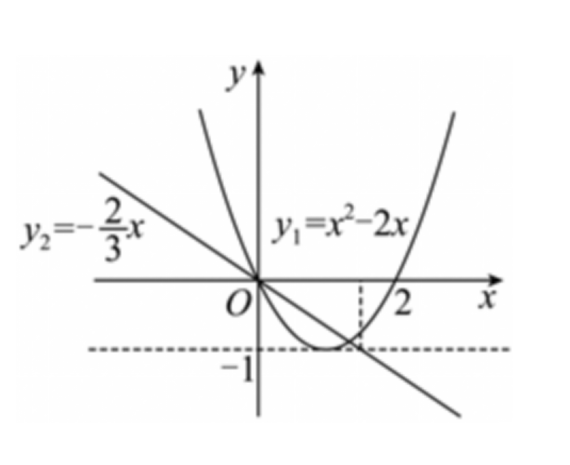
\includegraphics[width=0.24\textwidth]{figures/gao102_q7.png}
\end{center}
\step{当 $m>\dfrac32$ 时，当 $x>m$ 时 $f(x)\in\left(-\infty,-\dfrac23m\right)$，当 $x\leqslant m$ 时 $f(x)\in[-1,+\infty)$，}
\step{显然 $-\dfrac23m<-1$，此时函数 $f(x)$ 的值域不为 $R$，不符合题意；}
\step{当 $m<0$ 时，当 $x>m$ 时，$f(x)\in\left(-\infty,-\dfrac23m\right)$，}
\step{当 $x\leqslant m$ 时，$f(x)\in[m^2-2m,+\infty)$，}
\step{此时 $m^2-2m-\left(-\dfrac23m\right)=m^2-\dfrac43m=m\left(m-\dfrac43\right)>0$，即 $m^2-2m>-\dfrac23m$，}
\step{此时函数 $f(x)$ 的值域不为 $R$，不符合题意；}
\step{当 $0\leqslant m\leqslant\dfrac43$ 时，在 $x\in(0,m)$ 时 $y_2>y_1$，即 $m^2-2m<-\dfrac23m$，}
\step{此时 $f(x)$ 的值域为 $R$，符合题意，}
\step{当 $\dfrac43<m\leqslant\dfrac32$ 时，当 $x>m$ 时，$f(x)\in\left(-\infty,-\dfrac23m\right)$，}
\step{当 $x\leqslant m$ 时，$f(x)\in[-1,+\infty)$，}
\step{此时 $-1-\left(-\dfrac23m\right)=\dfrac23m-1\leqslant0$，即 $-1\leqslant-\dfrac23m$，}
\step{此时函数 $f(x)$ 的值域为 $R$，符合题意；}
\step{综上，$0\leqslant m\leqslant\dfrac32$，即实数 $m$ 的取值范围是 $\left[0,\dfrac32\right]$.}
\solend

\fi

\item 已知函数 $f(x)=x^2-2ax+b$（$a>1$）的定义域和值域都为 $[1,a]$，则 $b=$\blankline[4.4em].

\ifanswer
\solbegin
\step{$f(x)=x^2-2ax+b$（$a>1$）在 $[1,a]$ 严格减，}
\step{则 $f(1)=1-2a+b=a,f(a)=-a^2+b=1$，解得 $a=2,b=5$，所以 $b=5$.}
\solend

\fi

\item 若 $f(x)$ 满足 $f(x+y)=f(x)f(y)$，当 $x>0$ 时，$f(x)$ 的值域为 $(1,+\infty)$，则 $x<0$ 时，
$f(x)$ 的取值范围为\blankline[4.4em].

\ifanswer
\solbegin
\step{因为 $f(x+y)=f(x)f(y)$，令 $x=1$，$y=0$，得 $f(1+0)=f(1)f(0)$，}
\step{又因为当 $x>0$ 时，$f(x)>1$，所以 $f(1)>1>0$，故 $f(0)=1$.}
\step{当 $x<0$ 时，$-x>0$，令 $y=-x$，得 $f(x-x)=f(0)=1=f(x)f(-x)$，}
\step{故 $f(x)=\dfrac1{f(-x)}\in(0,1)$，故 $x<0$ 时，$f(x)$ 的取值范围为 $(0,1)$.}
\solend

\fi

\item 设函数 $f(x)=\begin{cases}x^2+x, & x<0\\ -x^2, & x\geqslant0\end{cases}$，若 $f(f(a))\leqslant2$，则实数 $a$ 的取值范围是\blankline[4.4em].

\ifanswer
\solbegin
\step{函数 $f(x)=\begin{cases}x^2+x, & x<0\\ -x^2, & x\geqslant0\end{cases}$，它的图象如图所示：}
\begin{center}
% 原图第 4 页解析插图直接裁取（原卷排于解析行右侧）。
% 裁框取图形区域，已去粉色水印转灰度。
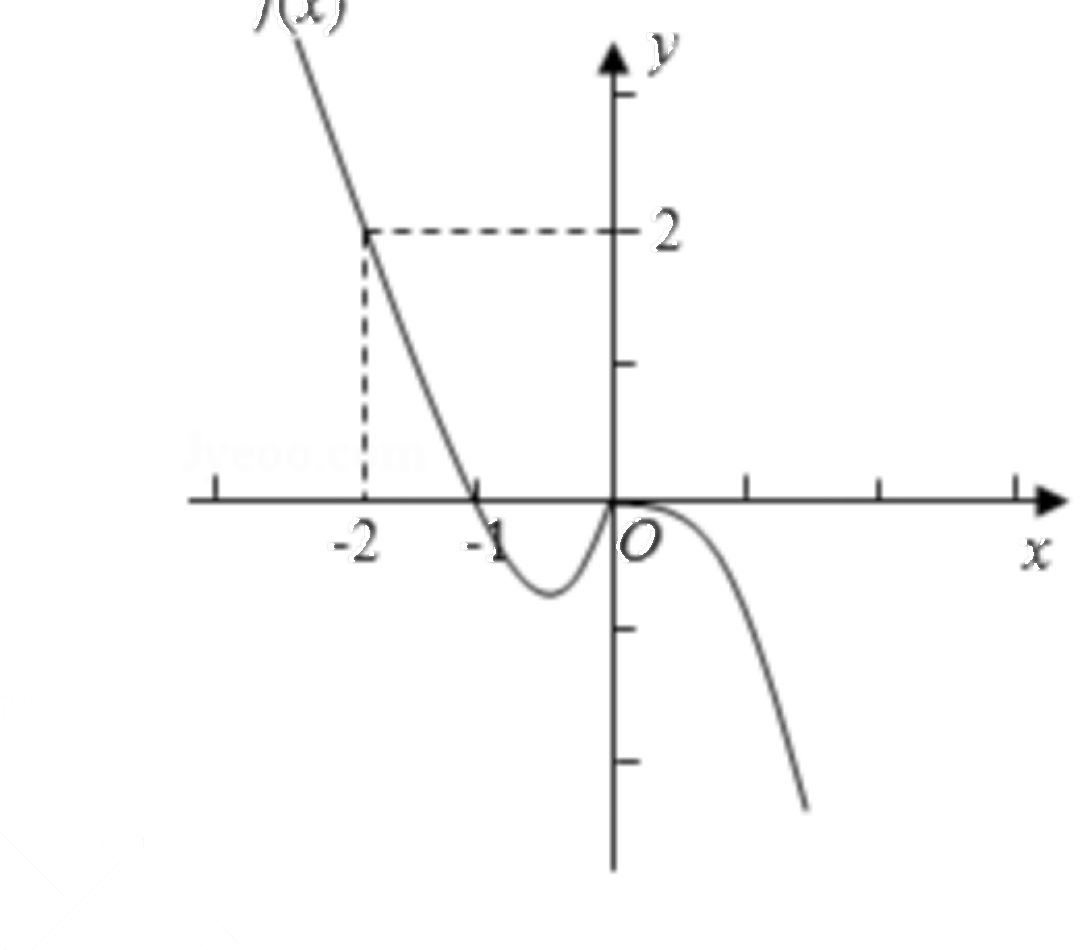
\includegraphics[width=0.30\textwidth]{figures/gao102_q10.png}
\end{center}
\step{由 $f(f(a))\leqslant2$，得 $f(a)\geqslant-2$.}
\step{当 $a<0$ 时，$f(a)=a^2+a=\left(a+\dfrac12\right)^2-\dfrac14\geqslant-2$ 恒成立；}
\step{当 $a\geqslant0$ 时，$f(a)=-a^2\geqslant-2$，即 $a^2\leqslant2$，解得 $0\leqslant a\leqslant\sqrt2$，}
\step{则实数 $a$ 的取值范围是 $(-\infty,\sqrt2]$.}
\solend

\fi

\item 已知二次函数 $f(x)$、$g(x)$ 的二次项系数均为 1，且满足
$\dfrac{f(2025)}{g(2025)}=\dfrac{f(2026)}{g(2026)}=\dfrac{2026}{2025}$，
则 $2026g(2027)-2025f(2027)$ 的值为\blankline[4.4em].

\ifanswer
\solbegin
\step{令 $h(x)=2026g(x)-2025f(x)$，其二次项系数为 $2026-2025=1$.}
\step{由比例条件得 $h(2025)=h(2026)=0$，}
\step{因此 $h(x)=(x-2025)(x-2026),h(2027)=2\times1=2$.}
\solend

\fi

\item 已知函数 $f(x)=\left\lvert x+\dfrac1x-a\right\rvert+1$，对任意实数 $x_1$、$x_2$、$x_3\in\left[\dfrac13,3\right]$，使得以
$f(x_1)$、$f(x_2)$、$f(x_3)$ 数值为边长可构成三角形，则实数 $a$ 的取值范围为\blankline[4.4em].

\ifanswer
\solbegin
\step{对任意实数 $x_1,x_2,x_3\in\left[\dfrac13,3\right]$，}
\step{使得以 $f(x_1)$、$f(x_2)$、$f(x_3)$ 数值为边长可构成三角形，}
\step{只需 $2f(x)_{\min}>f(x)_{\max}$，设 $g(x)=x+\dfrac1x-a$，}
\step{当 $x\in\left[\dfrac13,1\right)$ 时，函数 $g(x)$ 严格减，当 $x\in(1,3]$ 时，函数 $g(x)$ 严格增，}
\step{因为 $g(1)=2-a,g(3)=\dfrac{10}3-a,g\left(\dfrac13\right)=\dfrac{10}3-a$，所以 $g(x)\in\left[2-a,\dfrac{10}3-a\right]$，}
\step{当 $2-a\geqslant0$ 时，即 $a\leqslant2$ 时，$f(x)=\left\lvert x+\dfrac1x-a\right\rvert+1=g(x)+1$，}
\step{此时 $f(x)\in\left[3-a,\dfrac{13}3-a\right]$，}
\step{因此由 $2f(x)_{\min}>f(x)_{\max}\Rightarrow2(3-a)>\dfrac{13}3-a\Rightarrow a<\dfrac53$，而 $a\leqslant2$，所以 $a<\dfrac53$；}
\step{当 $\dfrac{10}3-a\leqslant0$，即 $a\geqslant\dfrac{10}3$ 时，$f(x)=\left\lvert x+\dfrac1x-a\right\rvert+1=-g(x)+1$，}
\step{此时 $f(x)\in\left[a-\dfrac73,a-1\right]$，}
\step{因此由 $2f(x)_{\min}>f(x)_{\max}\Rightarrow2\left(a-\dfrac73\right)>a-1\Rightarrow a>\dfrac{11}3$，而 $a\geqslant\dfrac{10}3$，所以 $a>\dfrac{11}3$，}
\step{若 $2-a<0<\dfrac{10}3-a$ 时，即 $2<a<\dfrac{10}3$ 时，}
\step{若 $a-2\geqslant\dfrac{10}3-a\Rightarrow a\geqslant\dfrac83$，即当 $\dfrac83\leqslant a<\dfrac{10}3$ 时，}
\step{显然此时 $f(x)_{\min}=1$，$f(x)_{\max}=a-2+1=a-1$，}
\step{由 $2f(x)_{\min}>f(x)_{\max}\Rightarrow2\times1>a-1\Rightarrow a<3$，显然 $\dfrac83\leqslant a<3$，}
\step{若 $a-2<\dfrac{10}3-a\Rightarrow a<\dfrac83$，即当 $2<a<\dfrac83$ 时，}
\step{显然此时 $f(x)_{\min}=1,f(x)_{\max}=\dfrac{10}3-a+1=\dfrac{13}3-a$，}
\step{因此由 $2f(x)_{\min}>f(x)_{\max}\Rightarrow2\times1>\dfrac{13}3-a\Rightarrow a>\dfrac73$，而 $\dfrac73<a<\dfrac83$，}
\step{综上，实数 $a$ 的取值范围为 $\left(-\infty,\dfrac53\right)\cup\left(\dfrac73,3\right)\cup\left(\dfrac{11}3,+\infty\right)$.}
\solend

\fi

\end{enumerate}

\bigsec{二、选择题}

\begin{enumerate}
\setcounter{enumi}{12}

\item 已知 $f(x)$ 是定义在 $\R$ 上的奇函数，$g(x)$ 是定义在 $\R$ 上的偶函数，则\mbox{（\quad）}

\keepwithprev
A. $f(x)g(x)$ 是偶函数\qquad B. $f(g(x))$ 是奇函数

C. $f(x)-g(x)$ 是奇函数\qquad D. $g(f(x))$ 是偶函数

\ifanswer
\solbegin
\step{$g(f(x))$ 的定义域为 $\R$，且 $g(f(-x))=g(-f(x))=g(f(x))$，}
\step{所以 $g(f(x))$ 是偶函数，故选 $D$.}
\solend

\fi

\item 已知定义在 $R$ 上的偶函数 $f(x)=\lvert x-m+1\rvert-2$，若正实数 $a$、$b$ 满足 $f(a)+f(2b)=m$，
则 $\dfrac1a+\dfrac2b$ 的最小值为\mbox{（\quad）}

\keepwithprev
A. $\dfrac95$\qquad\qquad B. $9$\qquad\qquad C. $\dfrac85$\qquad\qquad D. $8$

\ifanswer
\solbegin
\step{因为 $f(x)=\lvert x-m+1\rvert-2$ 是偶函数，所以 $-m+1=0$，所以 $m=1$，}
\step{所以 $f(x)=\lvert x\rvert-2$，若正实数 $a$、$b$ 满足 $f(a)+f(2b)=m$，}
\step{则 $a-2+2b-2=1$，所以 $a+2b=5$，}
\step{所以 $\dfrac1a+\dfrac2b=\dfrac15(a+2b)\left(\dfrac1a+\dfrac2b\right)=\dfrac15\left(5+\dfrac{2a}b+\dfrac{2b}a\right)\geqslant\dfrac95$，}
\step{当且仅当 $a=b=\dfrac53$ 时取等号，则 $\dfrac1a+\dfrac2b$ 的最小值为 $\dfrac95$，故选 $A$.}
\solend

\fi

\item 设函数 $g(x)=x^2-2$（$x\in\R$），$f(x)=\begin{cases}g(x)+x+4, & x<g(x)\\ g(x)-x, & x\geqslant g(x)\end{cases}$，则 $f(x)$ 的值域是

\mbox{（\quad）}

\keepwithprev
A. $\left[-\dfrac94,0\right]\cup(1,+\infty)$\qquad\qquad B. $[0,+\infty)$

C. $\left[-\dfrac94,+\infty\right)$\qquad\qquad D. $\left[-\dfrac94,0\right]\cup(2,+\infty)$

\ifanswer
\solbegin
\step{当 $x<g(x)$，即 $x<x^2-2$，$(x-2)(x+1)>0$ 时，$x>2$ 或 $x<-1$，}
\step{$f(x)=g(x)+x+4=x^2-2+x+4=x^2+x+2=(x+0.5)^2+1.75$，}
\step{其最小值趋向于 $f(-1)$ 即 2，无最大值，}
\step{因此这个区间的值域为 $(2,+\infty)$.}
\step{当 $x\geqslant g(x)$ 时，$-1\leqslant x\leqslant2$，$f(x)=g(x)-x=x^2-2-x=(x-0.5)^2-2.25$，}
\step{其最小值为 $f(0.5)=-2.25$，其最大值为 $f(2)=0$，}
\step{因此这区间的值域为 $[-2.25,0]$.}
\step{综上，函数值域为 $\left[-\dfrac94,0\right]\cup(2,+\infty)$，故选 $D$.}
\solend

\fi

\item 设 $D$ 是含数 1 的有限实数集，$f(x)$ 是定义在 $D$ 上的函数，若 $f(x)$ 的图象绕原点逆时针
旋转 $\dfrac{\pi}{6}$ 与原图象重合，则在以下各项中，$f(1)$ 的可能取值只能是\mbox{（\quad）}

\keepwithprev
A. $\sqrt3$\qquad\qquad B. $\dfrac{\sqrt3}2$\qquad\qquad C. $\dfrac{\sqrt3}3$\qquad\qquad D. $0$

\ifanswer
\solbegin
\step{问题相当于圆上由 12 个点为一组，每次绕原点逆时针旋转 $\dfrac{\pi}{6}$ 个单位后与下一个点}
\step{会重合。我们可以通过代入和赋值的方法，当 $f(1)=\sqrt3$、$\dfrac{\sqrt3}3$、$0$ 时，}
\step{此时得到的圆心角为 $\dfrac{\pi}{3}$、$\dfrac{\pi}{6}$、$0$，然而此时 $x=0$ 或者 $x=1$ 时，}
\step{都有 2 个 $y$ 与之对应，而我们知道函数的定义就是要求一个 $x$ 只能对应一个 $y$，}
\step{因此只有当 $x=\dfrac{\sqrt3}2$，此时旋转 $\dfrac{\pi}{6}$，此时满足一个 $x$ 只会对应一个 $y$，故选 $B$.}
\solend

\fi

\end{enumerate}

\bigsec{三、解答题}

\begin{enumerate}
\setcounter{enumi}{16}

\item 求下列函数的值域.

（1）$y=\dfrac{2x^2-3x+5}{x-1}\left(x\in\left[\dfrac32,3\right]\right)$；

（2）$f(x)=\sqrt{x}-\sqrt{2-x}+\sqrt{x(2-x)}$.

\ansspace*[10]

\ifanswer
\solbegin
\stepm{（1）}{令 $t=x-1$，则 $t\in\left[\dfrac12,2\right]$，原函数化为 $Y(t)=2t+\dfrac4t+1$.}
\step{当 $0<u<v$ 时，$Y(v)-Y(u)=2(v-u)\left(1-\dfrac2{uv}\right)$，}
\step{所以 $Y$ 在 $\left[\dfrac12,\sqrt2\right]$ 上严格递减，在 $[\sqrt2,2]$ 上严格递增.}
\step{由 $Y(\sqrt2)=4\sqrt2+1,Y\left(\dfrac12\right)=10,Y(2)=7$，得值域为 $[4\sqrt2+1,10]$.}
\stepm{（2）}{定义域为 $[0,2]$.}
\step{令 $s=\sqrt{x}-\sqrt{2-x}$，$\sqrt{x}$ 与 $-\sqrt{2-x}$ 均随 $x$ 严格递增，}
\step{$s$ 从 $-\sqrt2$ 递增到 $\sqrt2$，即 $s\in[-\sqrt2,\sqrt2]$.}
\step{由 $s^2=2-2\sqrt{x(2-x)}$，得 $f(x)=s+\dfrac{2-s^2}2=-\dfrac12(s-1)^2+\dfrac32$.}
\step{当 $s=1$ 时取得最大值 $\dfrac32$；当 $s=-\sqrt2$ 时取得最小值 $-\sqrt2$；}
\step{因此值域为 $\left[-\sqrt2,\dfrac32\right]$.}
\solend

\fi

\item 已知 $f(2x+1)=\dfrac{2x+1}{x+1}$.

（1）解不等式 $f(x)<x$；

（2）求 $f(1)+f(2)+\cdots+f(6)+f\left(\dfrac12\right)+f\left(\dfrac13\right)+\cdots+f\left(\dfrac16\right)$ 的值.

\ansspace*[12]

\ifanswer
\solbegin
\step{令 $t=2x+1$，则 $x=\dfrac{t-1}2$，得 $f(t)=\dfrac{2t}{t+1},t\neq-1$.}
\stepm{（1）}{不等式等价于 $\dfrac{2x}{x+1}<x\Leftrightarrow\dfrac{x(x-1)}{x+1}>0$.}
\step{以 $-1,0,1$ 分区间判断符号，得解集为 $(-1,0)\cup(1,+\infty)$.}
\stepm{（2）}{当 $x>0$ 时，$f(x)+f\left(\dfrac1x\right)=\dfrac{2x}{x+1}+\dfrac2{x+1}=2$.}
\step{将 $f(2),\cdots,f(6)$ 分别与其倒数对应的函数值配对，共 5 对，且 $f(1)=1$，}
\step{因此原式$=1+5\times2=11$.}
\solend

\fi

\item 已知函数 $f(x)$、$g(x)$ 是定义在 $R$ 上的函数，其中 $f(x)$ 是奇函数，$g(x)$ 是偶函数，且
$f(x)+g(x)=ax^2-x$.

（1）求 $f(x)$ 和 $g(x)$ 的解析式；

（2）$h(x)=f(x)+g(x)+(1-a)x^2-2ax+4$ 在 $[1,3]$ 上有两个零点，求实数 $a$ 的取值范
围.

\ansspace*[14]

\ifanswer
\solbegin
\stepm{（1）}{因为 $f(x)+g(x)=ax^2-x$①，所以 $f(-x)+g(-x)=ax^2+x$，}
\step{又 $f(x)$ 是奇函数，$g(x)$ 是偶函数，}
\step{所以 $f(-x)=-f(x)$，$g(-x)=g(x)$，}
\step{所以 $-f(x)+g(x)=ax^2+x$②，}
\step{联立①②解得 $f(x)=-x$，$g(x)=ax^2$.}
\stepm{（2）}{$h(x)=f(x)+g(x)+(1-a)x^2-2ax+4$}
\step{$=ax^2-x+(1-a)x^2-2ax+4=x^2-(2a+1)x+4$，}
\step{是开口向上，对称轴为 $x=\dfrac{2a+1}2$ 的二次函数，}
\step{因为 $h(x)$ 在 $[1,3]$ 上有两个零点，所以 $\begin{cases}\Delta=(2a+1)^2-16>0\\ 1<\dfrac{2a+1}2<3\\ h(1)=1-(2a+1)+4\geqslant0\\ h(3)=9-3(2a+1)+4\geqslant0\end{cases}$，}
\step{解得 $\dfrac32<a\leqslant\dfrac53$，故实数 $a$ 的取值范围为 $\left(\dfrac32,\dfrac53\right]$.}
\solend

\fi

\item 若函数 $f(x)$ 在区间 $[a,b]$ 上的值域恰为 $\left[\dfrac1b,\dfrac1a\right]$，则称区间 $[a,b]$ 为 $f(x)$ 的一个“倒域
区间”。已知定义在 $[-4,4]$ 上的奇函数 $g(x)$，当 $x\in[0,4]$ 时，$g(x)=-x^2+2x$.

（1）求 $g(x)$ 的解析式；

（2）若关于 $x$ 的方程 $g(x)=-mx-m$ 在 $(0,4)$ 上恰有两个不相等的实数根，求实数 $m$ 的
取值范围；

（3）求函数 $g(x)$ 在 $[-4,0]$ 内的“倒域区间”.

\ansspace*[16]

\ifanswer
\solbegin
\stepm{（1）}{当 $x\in[-4,0)$ 时，$-x\in(0,4]$，}
\step{由奇函数的定义得 $g(x)=-g(-x)=-[(-x)^2+2(-x)]=x^2+2x$，}
\step{所以 $g(x)=\begin{cases}-x^2+2x, & 0\leqslant x\leqslant4\\ x^2+2x, & -4\leqslant x<0\end{cases}$.}
\stepm{（2）}{方程 $g(x)=-mx-m$，即 $x^2-(m+2)x-m=0$，}
\step{设 $h(x)=x^2-(m+2)x-m$，$0<x<4$，}
\step{由题意得 $\begin{cases}h(0)=-m>0\\ h(4)=8-5m>0\\ \Delta=(m+2)^2+4m>0\\ 0<\dfrac{m+2}2<4\end{cases}$，解得 $2\sqrt3-4<m<0$，}
\step{即实数 $m$ 的取值范围是 $(2\sqrt3-4,0)$.}
\stepm{（3）}{易得当 $-4\leqslant a<b<0$ 时，$\dfrac1b<\dfrac1a$，}
\step{且 $g(x)$ 在 $[-4,-1]$ 上严格减，在 $[-1,0]$ 上严格增，}
\step{故当 $x\in[-4,0]$ 时，$g(x)_{\min}=g(-1)=-1$，}
\step{所以 $\dfrac1b\geqslant-1$，所以 $-4<b\leqslant-1$，所以 $-4\leqslant a<b\leqslant-1$，}
\step{则 $\begin{cases}g(a)=a^2+2a=\dfrac1a\\ g(b)=b^2+2b=\dfrac1b\\ -4\leqslant a<b\leqslant-1\end{cases}$，解得 $\begin{cases}a=-\dfrac{1+\sqrt5}2\\ b=-1\end{cases}$，}
\step{所以 $g(x)$ 在 $[-4,0]$ 内的“倒域区间”为 $\left[-\dfrac{1+\sqrt5}2,-1\right]$.}
\solend

\fi

\item 我们知道：函数 $y=f(x)$ 的图象关于坐标原点成中心对称图形的充要条件是函数
$y=f(x)$ 为奇函数。有同学发现可以推广为：函数 $y=f(x)$ 的图象关于点 $(a,b)$ 成中心对
称图形的充要条件为函数 $y=f(x+a)-b$ 为奇函数。已知函数 $f(x)=\dfrac{2x}{3-x}$.

（1）求函数 $f(x)$ 图象的对称中心；

（2）若定义在 $R$ 上的函数 $y=g(x)$ 的图象关于点 $(1,2)$ 对称，且 $g(1)=2$，当 $x\in[0,1)$
时，$g(x)=x^2-tx+t+1$.

（$i$）求 $g(-3)+g(5)$ 的值；

（$ii$）若对$\forall x_1\in[0,2]$，$\exists x_2\in[-3,2]$ 使得 $g(x_1)=f(x_2)$ 恒成立，求实数 $t$ 的取值范围.

\ansspace*[18]

\ifanswer
\solbegin
\stepm{（1）}{由 $f(x)=\dfrac{2x}{3-x}=-2+\dfrac6{3-x}$，}
\step{易得 $f(x+3)+2=-2+\dfrac6{3-(x+3)}+2=-\dfrac6x$ 为奇函数，}
\step{$f(x)$ 的图象关于 $(3,-2)$ 对称.}
\stepm{（2）}{（$i$）$y=g(x)$ 图象关于点 $(1,2)$ 对称，则 $g(1+x)+g(1-x)=4$，}
\step{令 $x=4$，则 $g(-3)+g(5)=4$.}
\step{（$ii$）有 $g(x)$ 在 $x\in[0,2]$ 的取值范围为 $f(x)$ 在 $x\in[-3,2]$ 的取值范围的}
\step{子集，}
\step{因为 $f(x)=\dfrac{2x}{3-x}=\dfrac{6-2(3-x)}{3-x}=\dfrac6{3-x}-2$ 在 $[-3,2]$ 上严格增，}
\step{所以 $f(x)$ 在 $x\in[-3,2]$ 上的取值范围为 $[-1,4]$，}
\step{记 $g(x)$ 的值域为 $A$，且 $g(1)=2$，当 $x\in[0,1)$ 时 $g(x)=x^2-tx+t+1$，}
\step{①当 $\dfrac t2\leqslant0$，即 $t\leqslant0$ 时，有 $g(x)$ 在 $[0,1)$ 上严格增，}
\step{由对称性得 $g(x)$ 在 $[1,2]$ 上严格增，故 $g(x)$ 在 $[0,2]$ 上严格增，}
\step{故 $g(x)_{\min}=g(0)=t+1$，$g(x)_{\max}=g(2)=4-(t+1)=3-t$，$t\leqslant0$，}
\step{则 $A=[t+1,3-t]\subseteq[-1,4]$，即 $\begin{cases}t\leqslant0\\ t+1\geqslant-1\\ 3-t\leqslant4\end{cases}$，解得 $-1\leqslant t\leqslant0$.}
\step{②当 $0<\dfrac t2<1$，即 $0<t<2$ 时，}
\step{$g(x)$ 在 $\left(0,\dfrac t2\right)$ 上严格减，在 $\left(\dfrac t2,1\right)$ 上严格增，}
\step{由对称性得 $g(x)$ 在 $\left(2-\dfrac t2,2\right)$ 上严格减，在 $\left(1,2-\dfrac t2\right)$ 上严格增，}
\step{故 $g(x)$ 在 $\left(0,\dfrac t2\right)$ 上严格减，在 $\left(\dfrac t2,2-\dfrac t2\right)$ 上严格增，}
\step{在 $\left(2-\dfrac t2,2\right)$ 上严格减，则 $A=\left[g\left(\dfrac t2\right),g\left(2-\dfrac t2\right)\right]$，}
\step{由 $0<t<2$，得 $g(0)=t+1\in(1,3)$，$g(2)=4-(t+1)=3-t\in(1,3)$，}
\step{$g\left(\dfrac t2\right)=-\dfrac{t^2}4+t+1=-\dfrac14(t-2)^2+2\in(1,2]$，}
\step{又 $g\left(\dfrac t2\right)+g\left(2-\dfrac t2\right)=4$，$g\left(2-\dfrac t2\right)\in(2,3)$，}
\step{当 $0<t<2$ 时，$A\subseteq[-1,4]$ 恒成立，}
\step{③当 $\dfrac t2\geqslant1$，即 $t\geqslant2$ 时，有 $g(x)$ 在 $[0,1)$ 上严格减，}
\step{由对称点 $(1,2)$ 得 $g(x)$ 在 $[1,2]$ 上严格减，所以 $g(x)$ 在 $[0,2]$ 上严格减，}
\step{故 $g(x)_{\max}=g(0)=t+1$，$g(x)_{\min}=g(2)=4-(t+1)=3-t$，$t\geqslant2$，}
\step{则 $A=[3-t,t+1]\subseteq[-1,4]$，即 $\begin{cases}t\geqslant2\\ t+1\leqslant4\\ 3-t\geqslant-1\end{cases}$，解得 $2\leqslant t\leqslant3$.}
\step{综上，$t$ 的范围为 $\{t\mid-1\leqslant t\leqslant3\}$.}
\solend

\fi

\end{enumerate}

\end{document}
"
%
% 原始材料：微信公众号“魔都数学加油站”文章，作者破晓，2026-11-01 21:56 发布；
% 连载“27学年高一102”，原文标题“27学年高一102——2026-2027年上海市华师大二附中高一上周末作业5函数”；
% 原文链接：https://mp.weixin.qq.com/s/CDvOCcxFskIe9aFUeKi3Ww。
% 正文为 13 张 PNG 页（第 1、2、10、13 页 2560×3620，其余 4762×6735），题目下印有【解析】，为讲评版。
% 题目、解析均据原图转录；卷面水印及公众号页脚未录入。
%
% 卷首标题：原卷印作“2026-2027 年华师大二附中高一上周末作业 5”（公众号标题中的“上海市”“函数”
% 卷面标题行没有，本稿照卷面），年份区间按全稿惯例排 en dash；原卷未印副标题，本稿按题目内容
% 标为“函数”（全稿首份以函数为单一模块的卷子）。
%
% 与原卷的排版差异：
%   ① 原文从第 3 题起，填空题编号为 3—12、选择题为 13—16、解答题为 17—21，本稿保留原题号；
%   ② 原卷每题下直接印【解析】，本稿按全稿惯例将解析置于答案版；选择题括号内未印答案，另由
%      解析末句“故选 X”给出；
%   ③ 原卷未印副标题，本稿按“知识模块”口径补出；
%   ④ 原卷填空横线按全稿惯例排为 \blankline[4.4em]；解答题按惯例加 \ansspace；选择题括号排
%      \mbox{（\quad）}、选项段前按惯例加 \keepwithprev；
%   ⑤ 原卷 $f(x)_{min}$、$f(x)_{max}$ 等下标排斜体，按 高一96 成例改正体 $\min$、$\max$；
%   ⑥ 原卷数集排斜体 $R$（第 13 题排粗体），按全稿惯例改 $\R$；
%   ⑦ 第 7、10 两题的解析插图裁自原图（去粉色水印转灰度），仅答案版显示。
%
% 原卷存疑／笔误（均照录加注）：
%   第 3 题解析“减去都对应 −2 和 2 的”措辞含糊（意为减去恒取 −2 与恒取 2 的两个常函数）；
%   第 15 题解析“其最小值趋向于 f(−1) 即 2”（该段 f(x)=x²+x+2 在 x→−1⁻ 时趋于 2、取不到）；
%   第 16 题解析末句“因此只有当 x=√3/2”（按上下文应为 f(1)=√3/2）；
%   第 16 题解析以 f(1)=√3、√3/3、0 赋值时称“得到的圆心角为 π/3、π/6、0”，其中 √3/3 对应
%   圆心角 π/6 的说法与该点 (1,√3/3) 的实际幅角一致，但与选项 C（√3/3）被排除的结论矛盾
%   （幅角 π/6 的点旋转 π/6 后落到幅角 π/3 处，仍占 12 等分点位，原卷解析未展开），照录。
%
% 行数核对：逐题数 \step/\stepm 条数，合计 155 条（Q3：2；Q4：3；Q5：6；Q6：5；Q7：19；
% Q8：2；Q9：4；Q10：5；Q11：3；Q12：19；Q13：2；Q14：5；Q15：8；Q16：5；Q17：10；
% Q18：6；Q19：10；Q20：13；Q21：28），与原卷印刷行逐题相等。
%
\documentclass[a4paper,11pt]{article}
\usepackage{common}

\begin{document}

\examtitlest[3]{2026--2027 年华师大二附中高一上周末作业 5}{函数}

\bigsec{一、填空题}

\begin{enumerate}
\setcounter{enumi}{2}

\item 已知函数 $y=f(x)$ 的定义域为 $\{-2,-1,1,2\}$，值域为 $\{-2,2\}$，则满足条件的函数
$y=f(x)$ 最多有\blankline[4.4em]个.

\ifanswer
\solbegin
\step{定义域中 4 个元素每个都可以对应 $-2$ 和 $2$ 中的一个，减去都对应 $-2$ 和 $2$ 的，}
\step{则满足条件的函数 $y=f(x)$ 最多有 $2^4-2=14$.}
\solend

\fi

\item 已知函数 $f(2x)$ 的定义域为 $[-2,2]$，则函数 $f(x-3)$ 的定义域为\blankline[4.4em].

\ifanswer
\solbegin
\step{因为函数 $f(2x)$ 的定义域为 $[-2,2]$，即 $-2\leqslant x\leqslant2$，所以 $-4\leqslant2x\leqslant4$，}
\step{得 $f(x)$ 的定义域为 $[-4,4]$，由 $-4\leqslant x-3\leqslant4$，解得 $-1\leqslant x\leqslant7$，}
\step{即函数 $f(x-3)$ 的定义域为 $[-1,7]$.}
\solend

\fi

\item 函数 $f(x)=\begin{cases}-x-1, & x<0\\ -x+1, & x>0\end{cases}$，则 $f(x)-f(-x)>1$ 的解集为\blankline[4.4em].

\ifanswer
\solbegin
\step{定义域为 $\{x\mid x\neq0\}$.}
\step{当 $x<0$ 时，$-x>0,f(-x)=x+1$，}
\step{$f(x)-f(-x)=(-x-1)-(x+1)=-2x-2>1$，得 $x<-\dfrac32$.}
\step{当 $x>0$ 时，$f(-x)=x-1,f(x)-f(-x)=(-x+1)-(x-1)=-2x+2>1$，}
\step{得 $0<x<\dfrac12$.}
\step{故解集为 $\left(-\infty,-\dfrac32\right)\cup\left(0,\dfrac12\right)$.}
\solend

\fi

\item 已知函数 $f(x)=x^2-2(m-3)x+5$ 在区间 $[2,+\infty)$ 上的最小值为 1，则实数 $m=$\blankline[4.4em].

\ifanswer
\solbegin
\step{函数 $f(x)$ 图象的对称轴为 $x=m-3$.}
\step{当 $m-3\leqslant2$，即 $m\leqslant5$ 时，$f(x)_{\min}=f(2)=9-4m+12=1$，解得 $m=5$；}
\step{当 $m-3>2$，即 $m>5$ 时，$f(x)_{\min}=f(m-3)=-m^2+6m-4=1$，}
\step{解得 $m=5$（舍去）或 $1$（舍去），}
\step{综上，$m=5$.}
\solend

\fi

\item 已知函数 $f(x)=\begin{cases}x^2-2x, & x\leqslant m\\ -\dfrac23x, & x>m\end{cases}$ 的值域为 $R$，则实数 $m$ 的取值范围是\blankline[4.4em].

\ifanswer
\solbegin
\step{对于函数 $y_1=x^2-2x$，则 $y_1=(x-1)^2-1\geqslant-1$，当且仅当 $x=1$ 时取等号，}
\step{且函数在 $(-\infty,1)$ 上严格减，在 $(1,+\infty)$ 上严格增，}
\step{对于函数 $y_2=-\dfrac23x$，令 $y_2=-1$，则 $x=\dfrac32$，且函数在定义域上严格减，}
\step{令 $x^2-2x=-\dfrac23x$，解得 $x=0$ 或 $x=\dfrac43$，}
\step{所以 $y_2=-\dfrac23x$ 与 $y_1=x^2-2x$ 的两个交点分别为 $(0,0)$、$\left(\dfrac43,-\dfrac89\right)$，}
\step{则函数 $y_2=-\dfrac23x$ 与 $y_1=x^2-2x$ 的图象如图所示：}
\begin{center}
% 原图第 2 页解析插图直接裁取（原卷排于解析行右侧）。
% 裁框取图形区域，已去粉色水印转灰度。
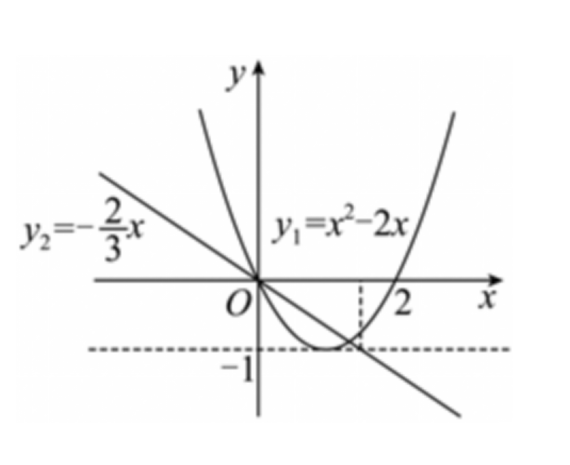
\includegraphics[width=0.24\textwidth]{figures/gao102_q7.png}
\end{center}
\step{当 $m>\dfrac32$ 时，当 $x>m$ 时 $f(x)\in\left(-\infty,-\dfrac23m\right)$，当 $x\leqslant m$ 时 $f(x)\in[-1,+\infty)$，}
\step{显然 $-\dfrac23m<-1$，此时函数 $f(x)$ 的值域不为 $R$，不符合题意；}
\step{当 $m<0$ 时，当 $x>m$ 时，$f(x)\in\left(-\infty,-\dfrac23m\right)$，}
\step{当 $x\leqslant m$ 时，$f(x)\in[m^2-2m,+\infty)$，}
\step{此时 $m^2-2m-\left(-\dfrac23m\right)=m^2-\dfrac43m=m\left(m-\dfrac43\right)>0$，即 $m^2-2m>-\dfrac23m$，}
\step{此时函数 $f(x)$ 的值域不为 $R$，不符合题意；}
\step{当 $0\leqslant m\leqslant\dfrac43$ 时，在 $x\in(0,m)$ 时 $y_2>y_1$，即 $m^2-2m<-\dfrac23m$，}
\step{此时 $f(x)$ 的值域为 $R$，符合题意，}
\step{当 $\dfrac43<m\leqslant\dfrac32$ 时，当 $x>m$ 时，$f(x)\in\left(-\infty,-\dfrac23m\right)$，}
\step{当 $x\leqslant m$ 时，$f(x)\in[-1,+\infty)$，}
\step{此时 $-1-\left(-\dfrac23m\right)=\dfrac23m-1\leqslant0$，即 $-1\leqslant-\dfrac23m$，}
\step{此时函数 $f(x)$ 的值域为 $R$，符合题意；}
\step{综上，$0\leqslant m\leqslant\dfrac32$，即实数 $m$ 的取值范围是 $\left[0,\dfrac32\right]$.}
\solend

\fi

\item 已知函数 $f(x)=x^2-2ax+b$（$a>1$）的定义域和值域都为 $[1,a]$，则 $b=$\blankline[4.4em].

\ifanswer
\solbegin
\step{$f(x)=x^2-2ax+b$（$a>1$）在 $[1,a]$ 严格减，}
\step{则 $f(1)=1-2a+b=a,f(a)=-a^2+b=1$，解得 $a=2,b=5$，所以 $b=5$.}
\solend

\fi

\item 若 $f(x)$ 满足 $f(x+y)=f(x)f(y)$，当 $x>0$ 时，$f(x)$ 的值域为 $(1,+\infty)$，则 $x<0$ 时，
$f(x)$ 的取值范围为\blankline[4.4em].

\ifanswer
\solbegin
\step{因为 $f(x+y)=f(x)f(y)$，令 $x=1$，$y=0$，得 $f(1+0)=f(1)f(0)$，}
\step{又因为当 $x>0$ 时，$f(x)>1$，所以 $f(1)>1>0$，故 $f(0)=1$.}
\step{当 $x<0$ 时，$-x>0$，令 $y=-x$，得 $f(x-x)=f(0)=1=f(x)f(-x)$，}
\step{故 $f(x)=\dfrac1{f(-x)}\in(0,1)$，故 $x<0$ 时，$f(x)$ 的取值范围为 $(0,1)$.}
\solend

\fi

\item 设函数 $f(x)=\begin{cases}x^2+x, & x<0\\ -x^2, & x\geqslant0\end{cases}$，若 $f(f(a))\leqslant2$，则实数 $a$ 的取值范围是\blankline[4.4em].

\ifanswer
\solbegin
\step{函数 $f(x)=\begin{cases}x^2+x, & x<0\\ -x^2, & x\geqslant0\end{cases}$，它的图象如图所示：}
\begin{center}
% 原图第 4 页解析插图直接裁取（原卷排于解析行右侧）。
% 裁框取图形区域，已去粉色水印转灰度。
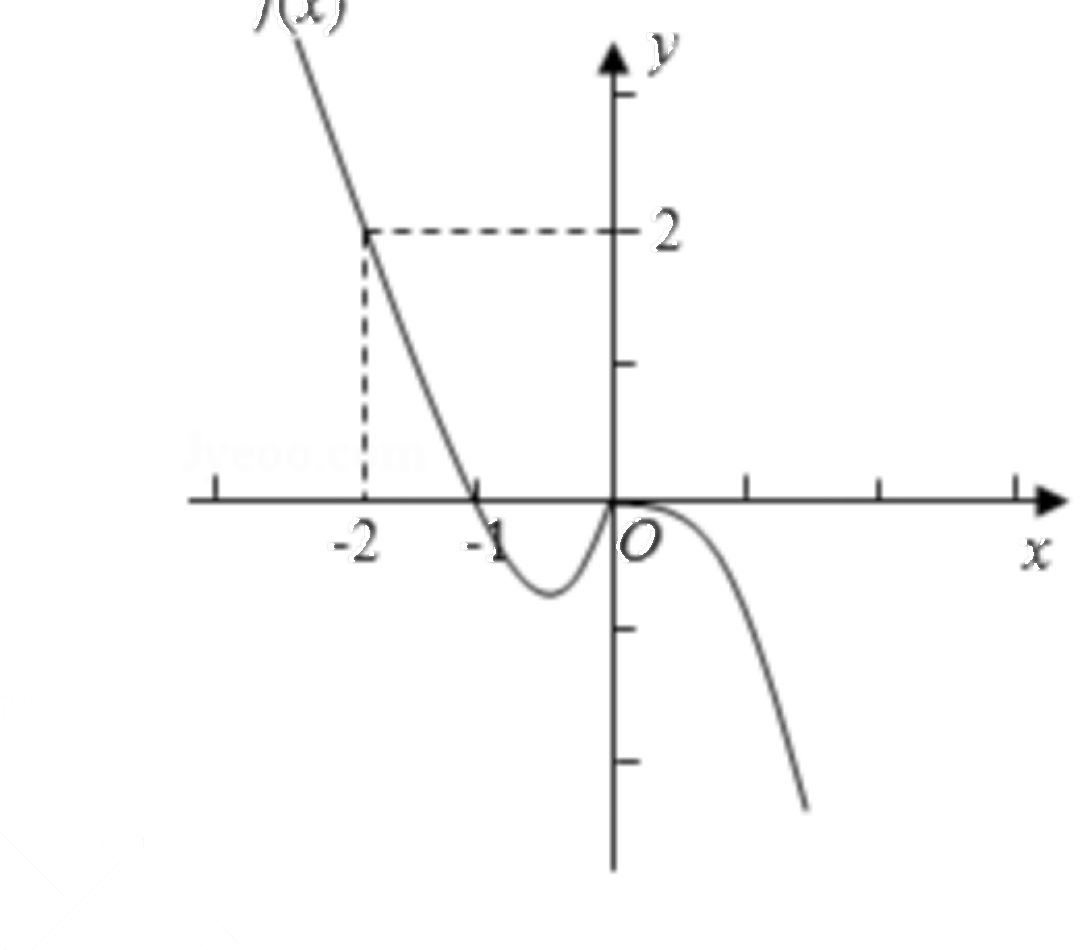
\includegraphics[width=0.30\textwidth]{figures/gao102_q10.png}
\end{center}
\step{由 $f(f(a))\leqslant2$，得 $f(a)\geqslant-2$.}
\step{当 $a<0$ 时，$f(a)=a^2+a=\left(a+\dfrac12\right)^2-\dfrac14\geqslant-2$ 恒成立；}
\step{当 $a\geqslant0$ 时，$f(a)=-a^2\geqslant-2$，即 $a^2\leqslant2$，解得 $0\leqslant a\leqslant\sqrt2$，}
\step{则实数 $a$ 的取值范围是 $(-\infty,\sqrt2]$.}
\solend

\fi

\item 已知二次函数 $f(x)$、$g(x)$ 的二次项系数均为 1，且满足
$\dfrac{f(2025)}{g(2025)}=\dfrac{f(2026)}{g(2026)}=\dfrac{2026}{2025}$，
则 $2026g(2027)-2025f(2027)$ 的值为\blankline[4.4em].

\ifanswer
\solbegin
\step{令 $h(x)=2026g(x)-2025f(x)$，其二次项系数为 $2026-2025=1$.}
\step{由比例条件得 $h(2025)=h(2026)=0$，}
\step{因此 $h(x)=(x-2025)(x-2026),h(2027)=2\times1=2$.}
\solend

\fi

\item 已知函数 $f(x)=\left\lvert x+\dfrac1x-a\right\rvert+1$，对任意实数 $x_1$、$x_2$、$x_3\in\left[\dfrac13,3\right]$，使得以
$f(x_1)$、$f(x_2)$、$f(x_3)$ 数值为边长可构成三角形，则实数 $a$ 的取值范围为\blankline[4.4em].

\ifanswer
\solbegin
\step{对任意实数 $x_1,x_2,x_3\in\left[\dfrac13,3\right]$，}
\step{使得以 $f(x_1)$、$f(x_2)$、$f(x_3)$ 数值为边长可构成三角形，}
\step{只需 $2f(x)_{\min}>f(x)_{\max}$，设 $g(x)=x+\dfrac1x-a$，}
\step{当 $x\in\left[\dfrac13,1\right)$ 时，函数 $g(x)$ 严格减，当 $x\in(1,3]$ 时，函数 $g(x)$ 严格增，}
\step{因为 $g(1)=2-a,g(3)=\dfrac{10}3-a,g\left(\dfrac13\right)=\dfrac{10}3-a$，所以 $g(x)\in\left[2-a,\dfrac{10}3-a\right]$，}
\step{当 $2-a\geqslant0$ 时，即 $a\leqslant2$ 时，$f(x)=\left\lvert x+\dfrac1x-a\right\rvert+1=g(x)+1$，}
\step{此时 $f(x)\in\left[3-a,\dfrac{13}3-a\right]$，}
\step{因此由 $2f(x)_{\min}>f(x)_{\max}\Rightarrow2(3-a)>\dfrac{13}3-a\Rightarrow a<\dfrac53$，而 $a\leqslant2$，所以 $a<\dfrac53$；}
\step{当 $\dfrac{10}3-a\leqslant0$，即 $a\geqslant\dfrac{10}3$ 时，$f(x)=\left\lvert x+\dfrac1x-a\right\rvert+1=-g(x)+1$，}
\step{此时 $f(x)\in\left[a-\dfrac73,a-1\right]$，}
\step{因此由 $2f(x)_{\min}>f(x)_{\max}\Rightarrow2\left(a-\dfrac73\right)>a-1\Rightarrow a>\dfrac{11}3$，而 $a\geqslant\dfrac{10}3$，所以 $a>\dfrac{11}3$，}
\step{若 $2-a<0<\dfrac{10}3-a$ 时，即 $2<a<\dfrac{10}3$ 时，}
\step{若 $a-2\geqslant\dfrac{10}3-a\Rightarrow a\geqslant\dfrac83$，即当 $\dfrac83\leqslant a<\dfrac{10}3$ 时，}
\step{显然此时 $f(x)_{\min}=1$，$f(x)_{\max}=a-2+1=a-1$，}
\step{由 $2f(x)_{\min}>f(x)_{\max}\Rightarrow2\times1>a-1\Rightarrow a<3$，显然 $\dfrac83\leqslant a<3$，}
\step{若 $a-2<\dfrac{10}3-a\Rightarrow a<\dfrac83$，即当 $2<a<\dfrac83$ 时，}
\step{显然此时 $f(x)_{\min}=1,f(x)_{\max}=\dfrac{10}3-a+1=\dfrac{13}3-a$，}
\step{因此由 $2f(x)_{\min}>f(x)_{\max}\Rightarrow2\times1>\dfrac{13}3-a\Rightarrow a>\dfrac73$，而 $\dfrac73<a<\dfrac83$，}
\step{综上，实数 $a$ 的取值范围为 $\left(-\infty,\dfrac53\right)\cup\left(\dfrac73,3\right)\cup\left(\dfrac{11}3,+\infty\right)$.}
\solend

\fi

\end{enumerate}

\bigsec{二、选择题}

\begin{enumerate}
\setcounter{enumi}{12}

\item 已知 $f(x)$ 是定义在 $\R$ 上的奇函数，$g(x)$ 是定义在 $\R$ 上的偶函数，则\mbox{（\quad）}

\keepwithprev
A. $f(x)g(x)$ 是偶函数\qquad B. $f(g(x))$ 是奇函数

C. $f(x)-g(x)$ 是奇函数\qquad D. $g(f(x))$ 是偶函数

\ifanswer
\solbegin
\step{$g(f(x))$ 的定义域为 $\R$，且 $g(f(-x))=g(-f(x))=g(f(x))$，}
\step{所以 $g(f(x))$ 是偶函数，故选 $D$.}
\solend

\fi

\item 已知定义在 $R$ 上的偶函数 $f(x)=\lvert x-m+1\rvert-2$，若正实数 $a$、$b$ 满足 $f(a)+f(2b)=m$，
则 $\dfrac1a+\dfrac2b$ 的最小值为\mbox{（\quad）}

\keepwithprev
A. $\dfrac95$\qquad\qquad B. $9$\qquad\qquad C. $\dfrac85$\qquad\qquad D. $8$

\ifanswer
\solbegin
\step{因为 $f(x)=\lvert x-m+1\rvert-2$ 是偶函数，所以 $-m+1=0$，所以 $m=1$，}
\step{所以 $f(x)=\lvert x\rvert-2$，若正实数 $a$、$b$ 满足 $f(a)+f(2b)=m$，}
\step{则 $a-2+2b-2=1$，所以 $a+2b=5$，}
\step{所以 $\dfrac1a+\dfrac2b=\dfrac15(a+2b)\left(\dfrac1a+\dfrac2b\right)=\dfrac15\left(5+\dfrac{2a}b+\dfrac{2b}a\right)\geqslant\dfrac95$，}
\step{当且仅当 $a=b=\dfrac53$ 时取等号，则 $\dfrac1a+\dfrac2b$ 的最小值为 $\dfrac95$，故选 $A$.}
\solend

\fi

\item 设函数 $g(x)=x^2-2$（$x\in\R$），$f(x)=\begin{cases}g(x)+x+4, & x<g(x)\\ g(x)-x, & x\geqslant g(x)\end{cases}$，则 $f(x)$ 的值域是

\mbox{（\quad）}

\keepwithprev
A. $\left[-\dfrac94,0\right]\cup(1,+\infty)$\qquad\qquad B. $[0,+\infty)$

C. $\left[-\dfrac94,+\infty\right)$\qquad\qquad D. $\left[-\dfrac94,0\right]\cup(2,+\infty)$

\ifanswer
\solbegin
\step{当 $x<g(x)$，即 $x<x^2-2$，$(x-2)(x+1)>0$ 时，$x>2$ 或 $x<-1$，}
\step{$f(x)=g(x)+x+4=x^2-2+x+4=x^2+x+2=(x+0.5)^2+1.75$，}
\step{其最小值趋向于 $f(-1)$ 即 2，无最大值，}
\step{因此这个区间的值域为 $(2,+\infty)$.}
\step{当 $x\geqslant g(x)$ 时，$-1\leqslant x\leqslant2$，$f(x)=g(x)-x=x^2-2-x=(x-0.5)^2-2.25$，}
\step{其最小值为 $f(0.5)=-2.25$，其最大值为 $f(2)=0$，}
\step{因此这区间的值域为 $[-2.25,0]$.}
\step{综上，函数值域为 $\left[-\dfrac94,0\right]\cup(2,+\infty)$，故选 $D$.}
\solend

\fi

\item 设 $D$ 是含数 1 的有限实数集，$f(x)$ 是定义在 $D$ 上的函数，若 $f(x)$ 的图象绕原点逆时针
旋转 $\dfrac{\pi}{6}$ 与原图象重合，则在以下各项中，$f(1)$ 的可能取值只能是\mbox{（\quad）}

\keepwithprev
A. $\sqrt3$\qquad\qquad B. $\dfrac{\sqrt3}2$\qquad\qquad C. $\dfrac{\sqrt3}3$\qquad\qquad D. $0$

\ifanswer
\solbegin
\step{问题相当于圆上由 12 个点为一组，每次绕原点逆时针旋转 $\dfrac{\pi}{6}$ 个单位后与下一个点}
\step{会重合。我们可以通过代入和赋值的方法，当 $f(1)=\sqrt3$、$\dfrac{\sqrt3}3$、$0$ 时，}
\step{此时得到的圆心角为 $\dfrac{\pi}{3}$、$\dfrac{\pi}{6}$、$0$，然而此时 $x=0$ 或者 $x=1$ 时，}
\step{都有 2 个 $y$ 与之对应，而我们知道函数的定义就是要求一个 $x$ 只能对应一个 $y$，}
\step{因此只有当 $x=\dfrac{\sqrt3}2$，此时旋转 $\dfrac{\pi}{6}$，此时满足一个 $x$ 只会对应一个 $y$，故选 $B$.}
\solend

\fi

\end{enumerate}

\bigsec{三、解答题}

\begin{enumerate}
\setcounter{enumi}{16}

\item 求下列函数的值域.

（1）$y=\dfrac{2x^2-3x+5}{x-1}\left(x\in\left[\dfrac32,3\right]\right)$；

（2）$f(x)=\sqrt{x}-\sqrt{2-x}+\sqrt{x(2-x)}$.

\ansspace*[10]

\ifanswer
\solbegin
\stepm{（1）}{令 $t=x-1$，则 $t\in\left[\dfrac12,2\right]$，原函数化为 $Y(t)=2t+\dfrac4t+1$.}
\step{当 $0<u<v$ 时，$Y(v)-Y(u)=2(v-u)\left(1-\dfrac2{uv}\right)$，}
\step{所以 $Y$ 在 $\left[\dfrac12,\sqrt2\right]$ 上严格递减，在 $[\sqrt2,2]$ 上严格递增.}
\step{由 $Y(\sqrt2)=4\sqrt2+1,Y\left(\dfrac12\right)=10,Y(2)=7$，得值域为 $[4\sqrt2+1,10]$.}
\stepm{（2）}{定义域为 $[0,2]$.}
\step{令 $s=\sqrt{x}-\sqrt{2-x}$，$\sqrt{x}$ 与 $-\sqrt{2-x}$ 均随 $x$ 严格递增，}
\step{$s$ 从 $-\sqrt2$ 递增到 $\sqrt2$，即 $s\in[-\sqrt2,\sqrt2]$.}
\step{由 $s^2=2-2\sqrt{x(2-x)}$，得 $f(x)=s+\dfrac{2-s^2}2=-\dfrac12(s-1)^2+\dfrac32$.}
\step{当 $s=1$ 时取得最大值 $\dfrac32$；当 $s=-\sqrt2$ 时取得最小值 $-\sqrt2$；}
\step{因此值域为 $\left[-\sqrt2,\dfrac32\right]$.}
\solend

\fi

\item 已知 $f(2x+1)=\dfrac{2x+1}{x+1}$.

（1）解不等式 $f(x)<x$；

（2）求 $f(1)+f(2)+\cdots+f(6)+f\left(\dfrac12\right)+f\left(\dfrac13\right)+\cdots+f\left(\dfrac16\right)$ 的值.

\ansspace*[12]

\ifanswer
\solbegin
\step{令 $t=2x+1$，则 $x=\dfrac{t-1}2$，得 $f(t)=\dfrac{2t}{t+1},t\neq-1$.}
\stepm{（1）}{不等式等价于 $\dfrac{2x}{x+1}<x\Leftrightarrow\dfrac{x(x-1)}{x+1}>0$.}
\step{以 $-1,0,1$ 分区间判断符号，得解集为 $(-1,0)\cup(1,+\infty)$.}
\stepm{（2）}{当 $x>0$ 时，$f(x)+f\left(\dfrac1x\right)=\dfrac{2x}{x+1}+\dfrac2{x+1}=2$.}
\step{将 $f(2),\cdots,f(6)$ 分别与其倒数对应的函数值配对，共 5 对，且 $f(1)=1$，}
\step{因此原式$=1+5\times2=11$.}
\solend

\fi

\item 已知函数 $f(x)$、$g(x)$ 是定义在 $R$ 上的函数，其中 $f(x)$ 是奇函数，$g(x)$ 是偶函数，且
$f(x)+g(x)=ax^2-x$.

（1）求 $f(x)$ 和 $g(x)$ 的解析式；

（2）$h(x)=f(x)+g(x)+(1-a)x^2-2ax+4$ 在 $[1,3]$ 上有两个零点，求实数 $a$ 的取值范
围.

\ansspace*[14]

\ifanswer
\solbegin
\stepm{（1）}{因为 $f(x)+g(x)=ax^2-x$①，所以 $f(-x)+g(-x)=ax^2+x$，}
\step{又 $f(x)$ 是奇函数，$g(x)$ 是偶函数，}
\step{所以 $f(-x)=-f(x)$，$g(-x)=g(x)$，}
\step{所以 $-f(x)+g(x)=ax^2+x$②，}
\step{联立①②解得 $f(x)=-x$，$g(x)=ax^2$.}
\stepm{（2）}{$h(x)=f(x)+g(x)+(1-a)x^2-2ax+4$}
\step{$=ax^2-x+(1-a)x^2-2ax+4=x^2-(2a+1)x+4$，}
\step{是开口向上，对称轴为 $x=\dfrac{2a+1}2$ 的二次函数，}
\step{因为 $h(x)$ 在 $[1,3]$ 上有两个零点，所以 $\begin{cases}\Delta=(2a+1)^2-16>0\\ 1<\dfrac{2a+1}2<3\\ h(1)=1-(2a+1)+4\geqslant0\\ h(3)=9-3(2a+1)+4\geqslant0\end{cases}$，}
\step{解得 $\dfrac32<a\leqslant\dfrac53$，故实数 $a$ 的取值范围为 $\left(\dfrac32,\dfrac53\right]$.}
\solend

\fi

\item 若函数 $f(x)$ 在区间 $[a,b]$ 上的值域恰为 $\left[\dfrac1b,\dfrac1a\right]$，则称区间 $[a,b]$ 为 $f(x)$ 的一个“倒域
区间”。已知定义在 $[-4,4]$ 上的奇函数 $g(x)$，当 $x\in[0,4]$ 时，$g(x)=-x^2+2x$.

（1）求 $g(x)$ 的解析式；

（2）若关于 $x$ 的方程 $g(x)=-mx-m$ 在 $(0,4)$ 上恰有两个不相等的实数根，求实数 $m$ 的
取值范围；

（3）求函数 $g(x)$ 在 $[-4,0]$ 内的“倒域区间”.

\ansspace*[16]

\ifanswer
\solbegin
\stepm{（1）}{当 $x\in[-4,0)$ 时，$-x\in(0,4]$，}
\step{由奇函数的定义得 $g(x)=-g(-x)=-[(-x)^2+2(-x)]=x^2+2x$，}
\step{所以 $g(x)=\begin{cases}-x^2+2x, & 0\leqslant x\leqslant4\\ x^2+2x, & -4\leqslant x<0\end{cases}$.}
\stepm{（2）}{方程 $g(x)=-mx-m$，即 $x^2-(m+2)x-m=0$，}
\step{设 $h(x)=x^2-(m+2)x-m$，$0<x<4$，}
\step{由题意得 $\begin{cases}h(0)=-m>0\\ h(4)=8-5m>0\\ \Delta=(m+2)^2+4m>0\\ 0<\dfrac{m+2}2<4\end{cases}$，解得 $2\sqrt3-4<m<0$，}
\step{即实数 $m$ 的取值范围是 $(2\sqrt3-4,0)$.}
\stepm{（3）}{易得当 $-4\leqslant a<b<0$ 时，$\dfrac1b<\dfrac1a$，}
\step{且 $g(x)$ 在 $[-4,-1]$ 上严格减，在 $[-1,0]$ 上严格增，}
\step{故当 $x\in[-4,0]$ 时，$g(x)_{\min}=g(-1)=-1$，}
\step{所以 $\dfrac1b\geqslant-1$，所以 $-4<b\leqslant-1$，所以 $-4\leqslant a<b\leqslant-1$，}
\step{则 $\begin{cases}g(a)=a^2+2a=\dfrac1a\\ g(b)=b^2+2b=\dfrac1b\\ -4\leqslant a<b\leqslant-1\end{cases}$，解得 $\begin{cases}a=-\dfrac{1+\sqrt5}2\\ b=-1\end{cases}$，}
\step{所以 $g(x)$ 在 $[-4,0]$ 内的“倒域区间”为 $\left[-\dfrac{1+\sqrt5}2,-1\right]$.}
\solend

\fi

\item 我们知道：函数 $y=f(x)$ 的图象关于坐标原点成中心对称图形的充要条件是函数
$y=f(x)$ 为奇函数。有同学发现可以推广为：函数 $y=f(x)$ 的图象关于点 $(a,b)$ 成中心对
称图形的充要条件为函数 $y=f(x+a)-b$ 为奇函数。已知函数 $f(x)=\dfrac{2x}{3-x}$.

（1）求函数 $f(x)$ 图象的对称中心；

（2）若定义在 $R$ 上的函数 $y=g(x)$ 的图象关于点 $(1,2)$ 对称，且 $g(1)=2$，当 $x\in[0,1)$
时，$g(x)=x^2-tx+t+1$.

（$i$）求 $g(-3)+g(5)$ 的值；

（$ii$）若对$\forall x_1\in[0,2]$，$\exists x_2\in[-3,2]$ 使得 $g(x_1)=f(x_2)$ 恒成立，求实数 $t$ 的取值范围.

\ansspace*[18]

\ifanswer
\solbegin
\stepm{（1）}{由 $f(x)=\dfrac{2x}{3-x}=-2+\dfrac6{3-x}$，}
\step{易得 $f(x+3)+2=-2+\dfrac6{3-(x+3)}+2=-\dfrac6x$ 为奇函数，}
\step{$f(x)$ 的图象关于 $(3,-2)$ 对称.}
\stepm{（2）}{（$i$）$y=g(x)$ 图象关于点 $(1,2)$ 对称，则 $g(1+x)+g(1-x)=4$，}
\step{令 $x=4$，则 $g(-3)+g(5)=4$.}
\step{（$ii$）有 $g(x)$ 在 $x\in[0,2]$ 的取值范围为 $f(x)$ 在 $x\in[-3,2]$ 的取值范围的}
\step{子集，}
\step{因为 $f(x)=\dfrac{2x}{3-x}=\dfrac{6-2(3-x)}{3-x}=\dfrac6{3-x}-2$ 在 $[-3,2]$ 上严格增，}
\step{所以 $f(x)$ 在 $x\in[-3,2]$ 上的取值范围为 $[-1,4]$，}
\step{记 $g(x)$ 的值域为 $A$，且 $g(1)=2$，当 $x\in[0,1)$ 时 $g(x)=x^2-tx+t+1$，}
\step{①当 $\dfrac t2\leqslant0$，即 $t\leqslant0$ 时，有 $g(x)$ 在 $[0,1)$ 上严格增，}
\step{由对称性得 $g(x)$ 在 $[1,2]$ 上严格增，故 $g(x)$ 在 $[0,2]$ 上严格增，}
\step{故 $g(x)_{\min}=g(0)=t+1$，$g(x)_{\max}=g(2)=4-(t+1)=3-t$，$t\leqslant0$，}
\step{则 $A=[t+1,3-t]\subseteq[-1,4]$，即 $\begin{cases}t\leqslant0\\ t+1\geqslant-1\\ 3-t\leqslant4\end{cases}$，解得 $-1\leqslant t\leqslant0$.}
\step{②当 $0<\dfrac t2<1$，即 $0<t<2$ 时，}
\step{$g(x)$ 在 $\left(0,\dfrac t2\right)$ 上严格减，在 $\left(\dfrac t2,1\right)$ 上严格增，}
\step{由对称性得 $g(x)$ 在 $\left(2-\dfrac t2,2\right)$ 上严格减，在 $\left(1,2-\dfrac t2\right)$ 上严格增，}
\step{故 $g(x)$ 在 $\left(0,\dfrac t2\right)$ 上严格减，在 $\left(\dfrac t2,2-\dfrac t2\right)$ 上严格增，}
\step{在 $\left(2-\dfrac t2,2\right)$ 上严格减，则 $A=\left[g\left(\dfrac t2\right),g\left(2-\dfrac t2\right)\right]$，}
\step{由 $0<t<2$，得 $g(0)=t+1\in(1,3)$，$g(2)=4-(t+1)=3-t\in(1,3)$，}
\step{$g\left(\dfrac t2\right)=-\dfrac{t^2}4+t+1=-\dfrac14(t-2)^2+2\in(1,2]$，}
\step{又 $g\left(\dfrac t2\right)+g\left(2-\dfrac t2\right)=4$，$g\left(2-\dfrac t2\right)\in(2,3)$，}
\step{当 $0<t<2$ 时，$A\subseteq[-1,4]$ 恒成立，}
\step{③当 $\dfrac t2\geqslant1$，即 $t\geqslant2$ 时，有 $g(x)$ 在 $[0,1)$ 上严格减，}
\step{由对称点 $(1,2)$ 得 $g(x)$ 在 $[1,2]$ 上严格减，所以 $g(x)$ 在 $[0,2]$ 上严格减，}
\step{故 $g(x)_{\max}=g(0)=t+1$，$g(x)_{\min}=g(2)=4-(t+1)=3-t$，$t\geqslant2$，}
\step{则 $A=[3-t,t+1]\subseteq[-1,4]$，即 $\begin{cases}t\geqslant2\\ t+1\leqslant4\\ 3-t\geqslant-1\end{cases}$，解得 $2\leqslant t\leqslant3$.}
\step{综上，$t$ 的范围为 $\{t\mid-1\leqslant t\leqslant3\}$.}
\solend

\fi

\end{enumerate}

\end{document}
"
% 紧凑版：xelatex "\def\iscompact{1}% 高一102_华师大二附中_周末作业5.tex
%   —— 高一上数学“2026-2027 年华师大二附中高一上周末作业 5”（试卷版/答案版）
% 试卷版：xelatex 高一102_华师大二附中_周末作业5.tex
% 答案版：xelatex "\def\isanswer{1}% 高一102_华师大二附中_周末作业5.tex
%   —— 高一上数学“2026-2027 年华师大二附中高一上周末作业 5”（试卷版/答案版）
% 试卷版：xelatex 高一102_华师大二附中_周末作业5.tex
% 答案版：xelatex "\def\isanswer{1}\input{高一102_华师大二附中_周末作业5.tex}"
% 紧凑版：xelatex "\def\iscompact{1}\input{高一102_华师大二附中_周末作业5.tex}"
%
% 原始材料：微信公众号“魔都数学加油站”文章，作者破晓，2026-11-01 21:56 发布；
% 连载“27学年高一102”，原文标题“27学年高一102——2026-2027年上海市华师大二附中高一上周末作业5函数”；
% 原文链接：https://mp.weixin.qq.com/s/CDvOCcxFskIe9aFUeKi3Ww。
% 正文为 13 张 PNG 页（第 1、2、10、13 页 2560×3620，其余 4762×6735），题目下印有【解析】，为讲评版。
% 题目、解析均据原图转录；卷面水印及公众号页脚未录入。
%
% 卷首标题：原卷印作“2026-2027 年华师大二附中高一上周末作业 5”（公众号标题中的“上海市”“函数”
% 卷面标题行没有，本稿照卷面），年份区间按全稿惯例排 en dash；原卷未印副标题，本稿按题目内容
% 标为“函数”（全稿首份以函数为单一模块的卷子）。
%
% 与原卷的排版差异：
%   ① 原文从第 3 题起，填空题编号为 3—12、选择题为 13—16、解答题为 17—21，本稿保留原题号；
%   ② 原卷每题下直接印【解析】，本稿按全稿惯例将解析置于答案版；选择题括号内未印答案，另由
%      解析末句“故选 X”给出；
%   ③ 原卷未印副标题，本稿按“知识模块”口径补出；
%   ④ 原卷填空横线按全稿惯例排为 \blankline[4.4em]；解答题按惯例加 \ansspace；选择题括号排
%      \mbox{（\quad）}、选项段前按惯例加 \keepwithprev；
%   ⑤ 原卷 $f(x)_{min}$、$f(x)_{max}$ 等下标排斜体，按 高一96 成例改正体 $\min$、$\max$；
%   ⑥ 原卷数集排斜体 $R$（第 13 题排粗体），按全稿惯例改 $\R$；
%   ⑦ 第 7、10 两题的解析插图裁自原图（去粉色水印转灰度），仅答案版显示。
%
% 原卷存疑／笔误（均照录加注）：
%   第 3 题解析“减去都对应 −2 和 2 的”措辞含糊（意为减去恒取 −2 与恒取 2 的两个常函数）；
%   第 15 题解析“其最小值趋向于 f(−1) 即 2”（该段 f(x)=x²+x+2 在 x→−1⁻ 时趋于 2、取不到）；
%   第 16 题解析末句“因此只有当 x=√3/2”（按上下文应为 f(1)=√3/2）；
%   第 16 题解析以 f(1)=√3、√3/3、0 赋值时称“得到的圆心角为 π/3、π/6、0”，其中 √3/3 对应
%   圆心角 π/6 的说法与该点 (1,√3/3) 的实际幅角一致，但与选项 C（√3/3）被排除的结论矛盾
%   （幅角 π/6 的点旋转 π/6 后落到幅角 π/3 处，仍占 12 等分点位，原卷解析未展开），照录。
%
% 行数核对：逐题数 \step/\stepm 条数，合计 155 条（Q3：2；Q4：3；Q5：6；Q6：5；Q7：19；
% Q8：2；Q9：4；Q10：5；Q11：3；Q12：19；Q13：2；Q14：5；Q15：8；Q16：5；Q17：10；
% Q18：6；Q19：10；Q20：13；Q21：28），与原卷印刷行逐题相等。
%
\documentclass[a4paper,11pt]{article}
\usepackage{common}

\begin{document}

\examtitlest[3]{2026--2027 年华师大二附中高一上周末作业 5}{函数}

\bigsec{一、填空题}

\begin{enumerate}
\setcounter{enumi}{2}

\item 已知函数 $y=f(x)$ 的定义域为 $\{-2,-1,1,2\}$，值域为 $\{-2,2\}$，则满足条件的函数
$y=f(x)$ 最多有\blankline[4.4em]个.

\ifanswer
\solbegin
\step{定义域中 4 个元素每个都可以对应 $-2$ 和 $2$ 中的一个，减去都对应 $-2$ 和 $2$ 的，}
\step{则满足条件的函数 $y=f(x)$ 最多有 $2^4-2=14$.}
\solend

\fi

\item 已知函数 $f(2x)$ 的定义域为 $[-2,2]$，则函数 $f(x-3)$ 的定义域为\blankline[4.4em].

\ifanswer
\solbegin
\step{因为函数 $f(2x)$ 的定义域为 $[-2,2]$，即 $-2\leqslant x\leqslant2$，所以 $-4\leqslant2x\leqslant4$，}
\step{得 $f(x)$ 的定义域为 $[-4,4]$，由 $-4\leqslant x-3\leqslant4$，解得 $-1\leqslant x\leqslant7$，}
\step{即函数 $f(x-3)$ 的定义域为 $[-1,7]$.}
\solend

\fi

\item 函数 $f(x)=\begin{cases}-x-1, & x<0\\ -x+1, & x>0\end{cases}$，则 $f(x)-f(-x)>1$ 的解集为\blankline[4.4em].

\ifanswer
\solbegin
\step{定义域为 $\{x\mid x\neq0\}$.}
\step{当 $x<0$ 时，$-x>0,f(-x)=x+1$，}
\step{$f(x)-f(-x)=(-x-1)-(x+1)=-2x-2>1$，得 $x<-\dfrac32$.}
\step{当 $x>0$ 时，$f(-x)=x-1,f(x)-f(-x)=(-x+1)-(x-1)=-2x+2>1$，}
\step{得 $0<x<\dfrac12$.}
\step{故解集为 $\left(-\infty,-\dfrac32\right)\cup\left(0,\dfrac12\right)$.}
\solend

\fi

\item 已知函数 $f(x)=x^2-2(m-3)x+5$ 在区间 $[2,+\infty)$ 上的最小值为 1，则实数 $m=$\blankline[4.4em].

\ifanswer
\solbegin
\step{函数 $f(x)$ 图象的对称轴为 $x=m-3$.}
\step{当 $m-3\leqslant2$，即 $m\leqslant5$ 时，$f(x)_{\min}=f(2)=9-4m+12=1$，解得 $m=5$；}
\step{当 $m-3>2$，即 $m>5$ 时，$f(x)_{\min}=f(m-3)=-m^2+6m-4=1$，}
\step{解得 $m=5$（舍去）或 $1$（舍去），}
\step{综上，$m=5$.}
\solend

\fi

\item 已知函数 $f(x)=\begin{cases}x^2-2x, & x\leqslant m\\ -\dfrac23x, & x>m\end{cases}$ 的值域为 $R$，则实数 $m$ 的取值范围是\blankline[4.4em].

\ifanswer
\solbegin
\step{对于函数 $y_1=x^2-2x$，则 $y_1=(x-1)^2-1\geqslant-1$，当且仅当 $x=1$ 时取等号，}
\step{且函数在 $(-\infty,1)$ 上严格减，在 $(1,+\infty)$ 上严格增，}
\step{对于函数 $y_2=-\dfrac23x$，令 $y_2=-1$，则 $x=\dfrac32$，且函数在定义域上严格减，}
\step{令 $x^2-2x=-\dfrac23x$，解得 $x=0$ 或 $x=\dfrac43$，}
\step{所以 $y_2=-\dfrac23x$ 与 $y_1=x^2-2x$ 的两个交点分别为 $(0,0)$、$\left(\dfrac43,-\dfrac89\right)$，}
\step{则函数 $y_2=-\dfrac23x$ 与 $y_1=x^2-2x$ 的图象如图所示：}
\begin{center}
% 原图第 2 页解析插图直接裁取（原卷排于解析行右侧）。
% 裁框取图形区域，已去粉色水印转灰度。
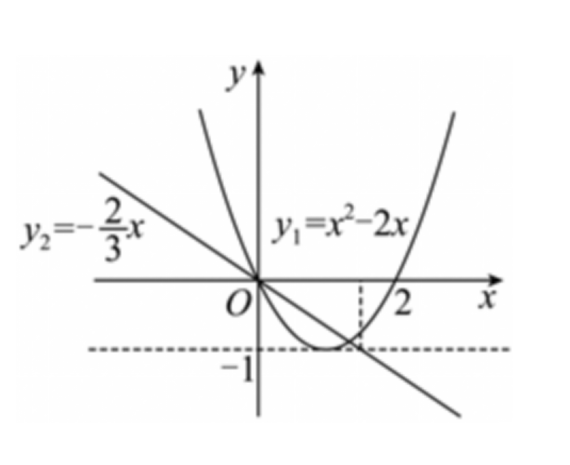
\includegraphics[width=0.24\textwidth]{figures/gao102_q7.png}
\end{center}
\step{当 $m>\dfrac32$ 时，当 $x>m$ 时 $f(x)\in\left(-\infty,-\dfrac23m\right)$，当 $x\leqslant m$ 时 $f(x)\in[-1,+\infty)$，}
\step{显然 $-\dfrac23m<-1$，此时函数 $f(x)$ 的值域不为 $R$，不符合题意；}
\step{当 $m<0$ 时，当 $x>m$ 时，$f(x)\in\left(-\infty,-\dfrac23m\right)$，}
\step{当 $x\leqslant m$ 时，$f(x)\in[m^2-2m,+\infty)$，}
\step{此时 $m^2-2m-\left(-\dfrac23m\right)=m^2-\dfrac43m=m\left(m-\dfrac43\right)>0$，即 $m^2-2m>-\dfrac23m$，}
\step{此时函数 $f(x)$ 的值域不为 $R$，不符合题意；}
\step{当 $0\leqslant m\leqslant\dfrac43$ 时，在 $x\in(0,m)$ 时 $y_2>y_1$，即 $m^2-2m<-\dfrac23m$，}
\step{此时 $f(x)$ 的值域为 $R$，符合题意，}
\step{当 $\dfrac43<m\leqslant\dfrac32$ 时，当 $x>m$ 时，$f(x)\in\left(-\infty,-\dfrac23m\right)$，}
\step{当 $x\leqslant m$ 时，$f(x)\in[-1,+\infty)$，}
\step{此时 $-1-\left(-\dfrac23m\right)=\dfrac23m-1\leqslant0$，即 $-1\leqslant-\dfrac23m$，}
\step{此时函数 $f(x)$ 的值域为 $R$，符合题意；}
\step{综上，$0\leqslant m\leqslant\dfrac32$，即实数 $m$ 的取值范围是 $\left[0,\dfrac32\right]$.}
\solend

\fi

\item 已知函数 $f(x)=x^2-2ax+b$（$a>1$）的定义域和值域都为 $[1,a]$，则 $b=$\blankline[4.4em].

\ifanswer
\solbegin
\step{$f(x)=x^2-2ax+b$（$a>1$）在 $[1,a]$ 严格减，}
\step{则 $f(1)=1-2a+b=a,f(a)=-a^2+b=1$，解得 $a=2,b=5$，所以 $b=5$.}
\solend

\fi

\item 若 $f(x)$ 满足 $f(x+y)=f(x)f(y)$，当 $x>0$ 时，$f(x)$ 的值域为 $(1,+\infty)$，则 $x<0$ 时，
$f(x)$ 的取值范围为\blankline[4.4em].

\ifanswer
\solbegin
\step{因为 $f(x+y)=f(x)f(y)$，令 $x=1$，$y=0$，得 $f(1+0)=f(1)f(0)$，}
\step{又因为当 $x>0$ 时，$f(x)>1$，所以 $f(1)>1>0$，故 $f(0)=1$.}
\step{当 $x<0$ 时，$-x>0$，令 $y=-x$，得 $f(x-x)=f(0)=1=f(x)f(-x)$，}
\step{故 $f(x)=\dfrac1{f(-x)}\in(0,1)$，故 $x<0$ 时，$f(x)$ 的取值范围为 $(0,1)$.}
\solend

\fi

\item 设函数 $f(x)=\begin{cases}x^2+x, & x<0\\ -x^2, & x\geqslant0\end{cases}$，若 $f(f(a))\leqslant2$，则实数 $a$ 的取值范围是\blankline[4.4em].

\ifanswer
\solbegin
\step{函数 $f(x)=\begin{cases}x^2+x, & x<0\\ -x^2, & x\geqslant0\end{cases}$，它的图象如图所示：}
\begin{center}
% 原图第 4 页解析插图直接裁取（原卷排于解析行右侧）。
% 裁框取图形区域，已去粉色水印转灰度。
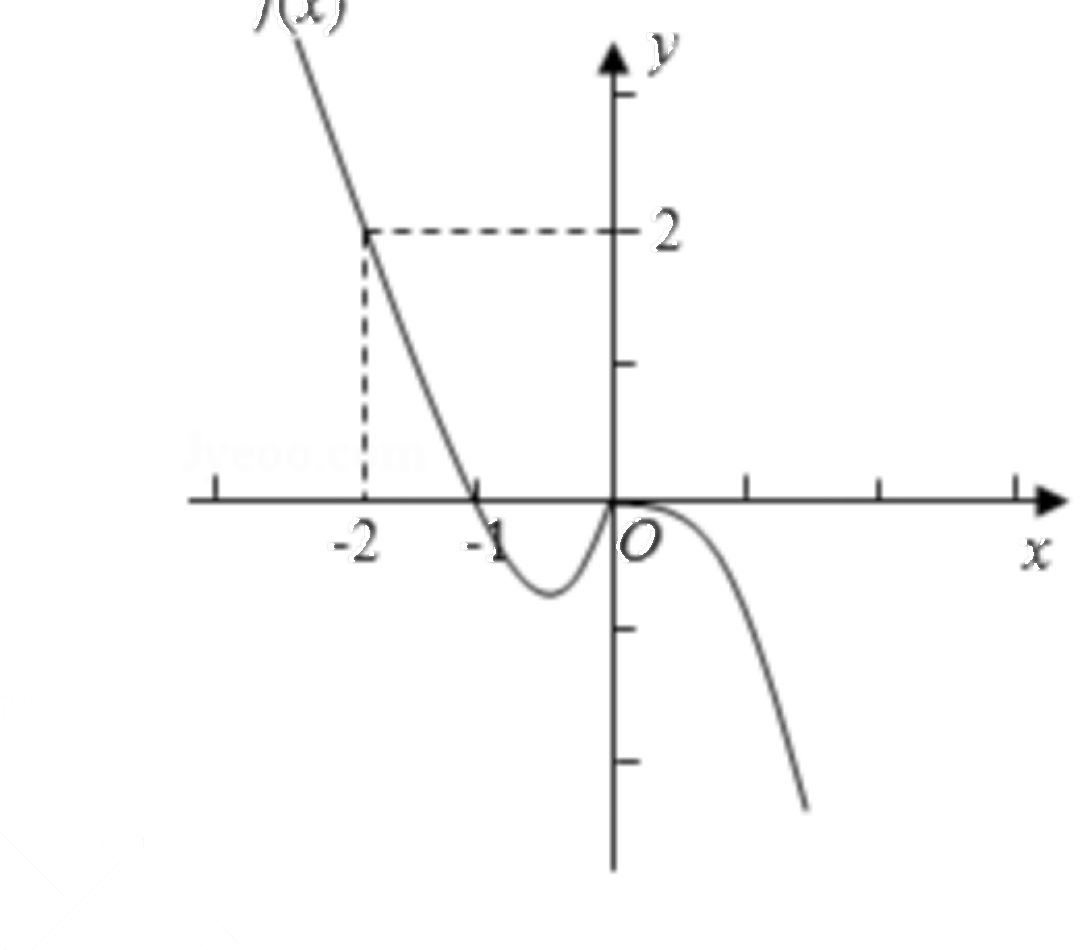
\includegraphics[width=0.30\textwidth]{figures/gao102_q10.png}
\end{center}
\step{由 $f(f(a))\leqslant2$，得 $f(a)\geqslant-2$.}
\step{当 $a<0$ 时，$f(a)=a^2+a=\left(a+\dfrac12\right)^2-\dfrac14\geqslant-2$ 恒成立；}
\step{当 $a\geqslant0$ 时，$f(a)=-a^2\geqslant-2$，即 $a^2\leqslant2$，解得 $0\leqslant a\leqslant\sqrt2$，}
\step{则实数 $a$ 的取值范围是 $(-\infty,\sqrt2]$.}
\solend

\fi

\item 已知二次函数 $f(x)$、$g(x)$ 的二次项系数均为 1，且满足
$\dfrac{f(2025)}{g(2025)}=\dfrac{f(2026)}{g(2026)}=\dfrac{2026}{2025}$，
则 $2026g(2027)-2025f(2027)$ 的值为\blankline[4.4em].

\ifanswer
\solbegin
\step{令 $h(x)=2026g(x)-2025f(x)$，其二次项系数为 $2026-2025=1$.}
\step{由比例条件得 $h(2025)=h(2026)=0$，}
\step{因此 $h(x)=(x-2025)(x-2026),h(2027)=2\times1=2$.}
\solend

\fi

\item 已知函数 $f(x)=\left\lvert x+\dfrac1x-a\right\rvert+1$，对任意实数 $x_1$、$x_2$、$x_3\in\left[\dfrac13,3\right]$，使得以
$f(x_1)$、$f(x_2)$、$f(x_3)$ 数值为边长可构成三角形，则实数 $a$ 的取值范围为\blankline[4.4em].

\ifanswer
\solbegin
\step{对任意实数 $x_1,x_2,x_3\in\left[\dfrac13,3\right]$，}
\step{使得以 $f(x_1)$、$f(x_2)$、$f(x_3)$ 数值为边长可构成三角形，}
\step{只需 $2f(x)_{\min}>f(x)_{\max}$，设 $g(x)=x+\dfrac1x-a$，}
\step{当 $x\in\left[\dfrac13,1\right)$ 时，函数 $g(x)$ 严格减，当 $x\in(1,3]$ 时，函数 $g(x)$ 严格增，}
\step{因为 $g(1)=2-a,g(3)=\dfrac{10}3-a,g\left(\dfrac13\right)=\dfrac{10}3-a$，所以 $g(x)\in\left[2-a,\dfrac{10}3-a\right]$，}
\step{当 $2-a\geqslant0$ 时，即 $a\leqslant2$ 时，$f(x)=\left\lvert x+\dfrac1x-a\right\rvert+1=g(x)+1$，}
\step{此时 $f(x)\in\left[3-a,\dfrac{13}3-a\right]$，}
\step{因此由 $2f(x)_{\min}>f(x)_{\max}\Rightarrow2(3-a)>\dfrac{13}3-a\Rightarrow a<\dfrac53$，而 $a\leqslant2$，所以 $a<\dfrac53$；}
\step{当 $\dfrac{10}3-a\leqslant0$，即 $a\geqslant\dfrac{10}3$ 时，$f(x)=\left\lvert x+\dfrac1x-a\right\rvert+1=-g(x)+1$，}
\step{此时 $f(x)\in\left[a-\dfrac73,a-1\right]$，}
\step{因此由 $2f(x)_{\min}>f(x)_{\max}\Rightarrow2\left(a-\dfrac73\right)>a-1\Rightarrow a>\dfrac{11}3$，而 $a\geqslant\dfrac{10}3$，所以 $a>\dfrac{11}3$，}
\step{若 $2-a<0<\dfrac{10}3-a$ 时，即 $2<a<\dfrac{10}3$ 时，}
\step{若 $a-2\geqslant\dfrac{10}3-a\Rightarrow a\geqslant\dfrac83$，即当 $\dfrac83\leqslant a<\dfrac{10}3$ 时，}
\step{显然此时 $f(x)_{\min}=1$，$f(x)_{\max}=a-2+1=a-1$，}
\step{由 $2f(x)_{\min}>f(x)_{\max}\Rightarrow2\times1>a-1\Rightarrow a<3$，显然 $\dfrac83\leqslant a<3$，}
\step{若 $a-2<\dfrac{10}3-a\Rightarrow a<\dfrac83$，即当 $2<a<\dfrac83$ 时，}
\step{显然此时 $f(x)_{\min}=1,f(x)_{\max}=\dfrac{10}3-a+1=\dfrac{13}3-a$，}
\step{因此由 $2f(x)_{\min}>f(x)_{\max}\Rightarrow2\times1>\dfrac{13}3-a\Rightarrow a>\dfrac73$，而 $\dfrac73<a<\dfrac83$，}
\step{综上，实数 $a$ 的取值范围为 $\left(-\infty,\dfrac53\right)\cup\left(\dfrac73,3\right)\cup\left(\dfrac{11}3,+\infty\right)$.}
\solend

\fi

\end{enumerate}

\bigsec{二、选择题}

\begin{enumerate}
\setcounter{enumi}{12}

\item 已知 $f(x)$ 是定义在 $\R$ 上的奇函数，$g(x)$ 是定义在 $\R$ 上的偶函数，则\mbox{（\quad）}

\keepwithprev
A. $f(x)g(x)$ 是偶函数\qquad B. $f(g(x))$ 是奇函数

C. $f(x)-g(x)$ 是奇函数\qquad D. $g(f(x))$ 是偶函数

\ifanswer
\solbegin
\step{$g(f(x))$ 的定义域为 $\R$，且 $g(f(-x))=g(-f(x))=g(f(x))$，}
\step{所以 $g(f(x))$ 是偶函数，故选 $D$.}
\solend

\fi

\item 已知定义在 $R$ 上的偶函数 $f(x)=\lvert x-m+1\rvert-2$，若正实数 $a$、$b$ 满足 $f(a)+f(2b)=m$，
则 $\dfrac1a+\dfrac2b$ 的最小值为\mbox{（\quad）}

\keepwithprev
A. $\dfrac95$\qquad\qquad B. $9$\qquad\qquad C. $\dfrac85$\qquad\qquad D. $8$

\ifanswer
\solbegin
\step{因为 $f(x)=\lvert x-m+1\rvert-2$ 是偶函数，所以 $-m+1=0$，所以 $m=1$，}
\step{所以 $f(x)=\lvert x\rvert-2$，若正实数 $a$、$b$ 满足 $f(a)+f(2b)=m$，}
\step{则 $a-2+2b-2=1$，所以 $a+2b=5$，}
\step{所以 $\dfrac1a+\dfrac2b=\dfrac15(a+2b)\left(\dfrac1a+\dfrac2b\right)=\dfrac15\left(5+\dfrac{2a}b+\dfrac{2b}a\right)\geqslant\dfrac95$，}
\step{当且仅当 $a=b=\dfrac53$ 时取等号，则 $\dfrac1a+\dfrac2b$ 的最小值为 $\dfrac95$，故选 $A$.}
\solend

\fi

\item 设函数 $g(x)=x^2-2$（$x\in\R$），$f(x)=\begin{cases}g(x)+x+4, & x<g(x)\\ g(x)-x, & x\geqslant g(x)\end{cases}$，则 $f(x)$ 的值域是

\mbox{（\quad）}

\keepwithprev
A. $\left[-\dfrac94,0\right]\cup(1,+\infty)$\qquad\qquad B. $[0,+\infty)$

C. $\left[-\dfrac94,+\infty\right)$\qquad\qquad D. $\left[-\dfrac94,0\right]\cup(2,+\infty)$

\ifanswer
\solbegin
\step{当 $x<g(x)$，即 $x<x^2-2$，$(x-2)(x+1)>0$ 时，$x>2$ 或 $x<-1$，}
\step{$f(x)=g(x)+x+4=x^2-2+x+4=x^2+x+2=(x+0.5)^2+1.75$，}
\step{其最小值趋向于 $f(-1)$ 即 2，无最大值，}
\step{因此这个区间的值域为 $(2,+\infty)$.}
\step{当 $x\geqslant g(x)$ 时，$-1\leqslant x\leqslant2$，$f(x)=g(x)-x=x^2-2-x=(x-0.5)^2-2.25$，}
\step{其最小值为 $f(0.5)=-2.25$，其最大值为 $f(2)=0$，}
\step{因此这区间的值域为 $[-2.25,0]$.}
\step{综上，函数值域为 $\left[-\dfrac94,0\right]\cup(2,+\infty)$，故选 $D$.}
\solend

\fi

\item 设 $D$ 是含数 1 的有限实数集，$f(x)$ 是定义在 $D$ 上的函数，若 $f(x)$ 的图象绕原点逆时针
旋转 $\dfrac{\pi}{6}$ 与原图象重合，则在以下各项中，$f(1)$ 的可能取值只能是\mbox{（\quad）}

\keepwithprev
A. $\sqrt3$\qquad\qquad B. $\dfrac{\sqrt3}2$\qquad\qquad C. $\dfrac{\sqrt3}3$\qquad\qquad D. $0$

\ifanswer
\solbegin
\step{问题相当于圆上由 12 个点为一组，每次绕原点逆时针旋转 $\dfrac{\pi}{6}$ 个单位后与下一个点}
\step{会重合。我们可以通过代入和赋值的方法，当 $f(1)=\sqrt3$、$\dfrac{\sqrt3}3$、$0$ 时，}
\step{此时得到的圆心角为 $\dfrac{\pi}{3}$、$\dfrac{\pi}{6}$、$0$，然而此时 $x=0$ 或者 $x=1$ 时，}
\step{都有 2 个 $y$ 与之对应，而我们知道函数的定义就是要求一个 $x$ 只能对应一个 $y$，}
\step{因此只有当 $x=\dfrac{\sqrt3}2$，此时旋转 $\dfrac{\pi}{6}$，此时满足一个 $x$ 只会对应一个 $y$，故选 $B$.}
\solend

\fi

\end{enumerate}

\bigsec{三、解答题}

\begin{enumerate}
\setcounter{enumi}{16}

\item 求下列函数的值域.

（1）$y=\dfrac{2x^2-3x+5}{x-1}\left(x\in\left[\dfrac32,3\right]\right)$；

（2）$f(x)=\sqrt{x}-\sqrt{2-x}+\sqrt{x(2-x)}$.

\ansspace*[10]

\ifanswer
\solbegin
\stepm{（1）}{令 $t=x-1$，则 $t\in\left[\dfrac12,2\right]$，原函数化为 $Y(t)=2t+\dfrac4t+1$.}
\step{当 $0<u<v$ 时，$Y(v)-Y(u)=2(v-u)\left(1-\dfrac2{uv}\right)$，}
\step{所以 $Y$ 在 $\left[\dfrac12,\sqrt2\right]$ 上严格递减，在 $[\sqrt2,2]$ 上严格递增.}
\step{由 $Y(\sqrt2)=4\sqrt2+1,Y\left(\dfrac12\right)=10,Y(2)=7$，得值域为 $[4\sqrt2+1,10]$.}
\stepm{（2）}{定义域为 $[0,2]$.}
\step{令 $s=\sqrt{x}-\sqrt{2-x}$，$\sqrt{x}$ 与 $-\sqrt{2-x}$ 均随 $x$ 严格递增，}
\step{$s$ 从 $-\sqrt2$ 递增到 $\sqrt2$，即 $s\in[-\sqrt2,\sqrt2]$.}
\step{由 $s^2=2-2\sqrt{x(2-x)}$，得 $f(x)=s+\dfrac{2-s^2}2=-\dfrac12(s-1)^2+\dfrac32$.}
\step{当 $s=1$ 时取得最大值 $\dfrac32$；当 $s=-\sqrt2$ 时取得最小值 $-\sqrt2$；}
\step{因此值域为 $\left[-\sqrt2,\dfrac32\right]$.}
\solend

\fi

\item 已知 $f(2x+1)=\dfrac{2x+1}{x+1}$.

（1）解不等式 $f(x)<x$；

（2）求 $f(1)+f(2)+\cdots+f(6)+f\left(\dfrac12\right)+f\left(\dfrac13\right)+\cdots+f\left(\dfrac16\right)$ 的值.

\ansspace*[12]

\ifanswer
\solbegin
\step{令 $t=2x+1$，则 $x=\dfrac{t-1}2$，得 $f(t)=\dfrac{2t}{t+1},t\neq-1$.}
\stepm{（1）}{不等式等价于 $\dfrac{2x}{x+1}<x\Leftrightarrow\dfrac{x(x-1)}{x+1}>0$.}
\step{以 $-1,0,1$ 分区间判断符号，得解集为 $(-1,0)\cup(1,+\infty)$.}
\stepm{（2）}{当 $x>0$ 时，$f(x)+f\left(\dfrac1x\right)=\dfrac{2x}{x+1}+\dfrac2{x+1}=2$.}
\step{将 $f(2),\cdots,f(6)$ 分别与其倒数对应的函数值配对，共 5 对，且 $f(1)=1$，}
\step{因此原式$=1+5\times2=11$.}
\solend

\fi

\item 已知函数 $f(x)$、$g(x)$ 是定义在 $R$ 上的函数，其中 $f(x)$ 是奇函数，$g(x)$ 是偶函数，且
$f(x)+g(x)=ax^2-x$.

（1）求 $f(x)$ 和 $g(x)$ 的解析式；

（2）$h(x)=f(x)+g(x)+(1-a)x^2-2ax+4$ 在 $[1,3]$ 上有两个零点，求实数 $a$ 的取值范
围.

\ansspace*[14]

\ifanswer
\solbegin
\stepm{（1）}{因为 $f(x)+g(x)=ax^2-x$①，所以 $f(-x)+g(-x)=ax^2+x$，}
\step{又 $f(x)$ 是奇函数，$g(x)$ 是偶函数，}
\step{所以 $f(-x)=-f(x)$，$g(-x)=g(x)$，}
\step{所以 $-f(x)+g(x)=ax^2+x$②，}
\step{联立①②解得 $f(x)=-x$，$g(x)=ax^2$.}
\stepm{（2）}{$h(x)=f(x)+g(x)+(1-a)x^2-2ax+4$}
\step{$=ax^2-x+(1-a)x^2-2ax+4=x^2-(2a+1)x+4$，}
\step{是开口向上，对称轴为 $x=\dfrac{2a+1}2$ 的二次函数，}
\step{因为 $h(x)$ 在 $[1,3]$ 上有两个零点，所以 $\begin{cases}\Delta=(2a+1)^2-16>0\\ 1<\dfrac{2a+1}2<3\\ h(1)=1-(2a+1)+4\geqslant0\\ h(3)=9-3(2a+1)+4\geqslant0\end{cases}$，}
\step{解得 $\dfrac32<a\leqslant\dfrac53$，故实数 $a$ 的取值范围为 $\left(\dfrac32,\dfrac53\right]$.}
\solend

\fi

\item 若函数 $f(x)$ 在区间 $[a,b]$ 上的值域恰为 $\left[\dfrac1b,\dfrac1a\right]$，则称区间 $[a,b]$ 为 $f(x)$ 的一个“倒域
区间”。已知定义在 $[-4,4]$ 上的奇函数 $g(x)$，当 $x\in[0,4]$ 时，$g(x)=-x^2+2x$.

（1）求 $g(x)$ 的解析式；

（2）若关于 $x$ 的方程 $g(x)=-mx-m$ 在 $(0,4)$ 上恰有两个不相等的实数根，求实数 $m$ 的
取值范围；

（3）求函数 $g(x)$ 在 $[-4,0]$ 内的“倒域区间”.

\ansspace*[16]

\ifanswer
\solbegin
\stepm{（1）}{当 $x\in[-4,0)$ 时，$-x\in(0,4]$，}
\step{由奇函数的定义得 $g(x)=-g(-x)=-[(-x)^2+2(-x)]=x^2+2x$，}
\step{所以 $g(x)=\begin{cases}-x^2+2x, & 0\leqslant x\leqslant4\\ x^2+2x, & -4\leqslant x<0\end{cases}$.}
\stepm{（2）}{方程 $g(x)=-mx-m$，即 $x^2-(m+2)x-m=0$，}
\step{设 $h(x)=x^2-(m+2)x-m$，$0<x<4$，}
\step{由题意得 $\begin{cases}h(0)=-m>0\\ h(4)=8-5m>0\\ \Delta=(m+2)^2+4m>0\\ 0<\dfrac{m+2}2<4\end{cases}$，解得 $2\sqrt3-4<m<0$，}
\step{即实数 $m$ 的取值范围是 $(2\sqrt3-4,0)$.}
\stepm{（3）}{易得当 $-4\leqslant a<b<0$ 时，$\dfrac1b<\dfrac1a$，}
\step{且 $g(x)$ 在 $[-4,-1]$ 上严格减，在 $[-1,0]$ 上严格增，}
\step{故当 $x\in[-4,0]$ 时，$g(x)_{\min}=g(-1)=-1$，}
\step{所以 $\dfrac1b\geqslant-1$，所以 $-4<b\leqslant-1$，所以 $-4\leqslant a<b\leqslant-1$，}
\step{则 $\begin{cases}g(a)=a^2+2a=\dfrac1a\\ g(b)=b^2+2b=\dfrac1b\\ -4\leqslant a<b\leqslant-1\end{cases}$，解得 $\begin{cases}a=-\dfrac{1+\sqrt5}2\\ b=-1\end{cases}$，}
\step{所以 $g(x)$ 在 $[-4,0]$ 内的“倒域区间”为 $\left[-\dfrac{1+\sqrt5}2,-1\right]$.}
\solend

\fi

\item 我们知道：函数 $y=f(x)$ 的图象关于坐标原点成中心对称图形的充要条件是函数
$y=f(x)$ 为奇函数。有同学发现可以推广为：函数 $y=f(x)$ 的图象关于点 $(a,b)$ 成中心对
称图形的充要条件为函数 $y=f(x+a)-b$ 为奇函数。已知函数 $f(x)=\dfrac{2x}{3-x}$.

（1）求函数 $f(x)$ 图象的对称中心；

（2）若定义在 $R$ 上的函数 $y=g(x)$ 的图象关于点 $(1,2)$ 对称，且 $g(1)=2$，当 $x\in[0,1)$
时，$g(x)=x^2-tx+t+1$.

（$i$）求 $g(-3)+g(5)$ 的值；

（$ii$）若对$\forall x_1\in[0,2]$，$\exists x_2\in[-3,2]$ 使得 $g(x_1)=f(x_2)$ 恒成立，求实数 $t$ 的取值范围.

\ansspace*[18]

\ifanswer
\solbegin
\stepm{（1）}{由 $f(x)=\dfrac{2x}{3-x}=-2+\dfrac6{3-x}$，}
\step{易得 $f(x+3)+2=-2+\dfrac6{3-(x+3)}+2=-\dfrac6x$ 为奇函数，}
\step{$f(x)$ 的图象关于 $(3,-2)$ 对称.}
\stepm{（2）}{（$i$）$y=g(x)$ 图象关于点 $(1,2)$ 对称，则 $g(1+x)+g(1-x)=4$，}
\step{令 $x=4$，则 $g(-3)+g(5)=4$.}
\step{（$ii$）有 $g(x)$ 在 $x\in[0,2]$ 的取值范围为 $f(x)$ 在 $x\in[-3,2]$ 的取值范围的}
\step{子集，}
\step{因为 $f(x)=\dfrac{2x}{3-x}=\dfrac{6-2(3-x)}{3-x}=\dfrac6{3-x}-2$ 在 $[-3,2]$ 上严格增，}
\step{所以 $f(x)$ 在 $x\in[-3,2]$ 上的取值范围为 $[-1,4]$，}
\step{记 $g(x)$ 的值域为 $A$，且 $g(1)=2$，当 $x\in[0,1)$ 时 $g(x)=x^2-tx+t+1$，}
\step{①当 $\dfrac t2\leqslant0$，即 $t\leqslant0$ 时，有 $g(x)$ 在 $[0,1)$ 上严格增，}
\step{由对称性得 $g(x)$ 在 $[1,2]$ 上严格增，故 $g(x)$ 在 $[0,2]$ 上严格增，}
\step{故 $g(x)_{\min}=g(0)=t+1$，$g(x)_{\max}=g(2)=4-(t+1)=3-t$，$t\leqslant0$，}
\step{则 $A=[t+1,3-t]\subseteq[-1,4]$，即 $\begin{cases}t\leqslant0\\ t+1\geqslant-1\\ 3-t\leqslant4\end{cases}$，解得 $-1\leqslant t\leqslant0$.}
\step{②当 $0<\dfrac t2<1$，即 $0<t<2$ 时，}
\step{$g(x)$ 在 $\left(0,\dfrac t2\right)$ 上严格减，在 $\left(\dfrac t2,1\right)$ 上严格增，}
\step{由对称性得 $g(x)$ 在 $\left(2-\dfrac t2,2\right)$ 上严格减，在 $\left(1,2-\dfrac t2\right)$ 上严格增，}
\step{故 $g(x)$ 在 $\left(0,\dfrac t2\right)$ 上严格减，在 $\left(\dfrac t2,2-\dfrac t2\right)$ 上严格增，}
\step{在 $\left(2-\dfrac t2,2\right)$ 上严格减，则 $A=\left[g\left(\dfrac t2\right),g\left(2-\dfrac t2\right)\right]$，}
\step{由 $0<t<2$，得 $g(0)=t+1\in(1,3)$，$g(2)=4-(t+1)=3-t\in(1,3)$，}
\step{$g\left(\dfrac t2\right)=-\dfrac{t^2}4+t+1=-\dfrac14(t-2)^2+2\in(1,2]$，}
\step{又 $g\left(\dfrac t2\right)+g\left(2-\dfrac t2\right)=4$，$g\left(2-\dfrac t2\right)\in(2,3)$，}
\step{当 $0<t<2$ 时，$A\subseteq[-1,4]$ 恒成立，}
\step{③当 $\dfrac t2\geqslant1$，即 $t\geqslant2$ 时，有 $g(x)$ 在 $[0,1)$ 上严格减，}
\step{由对称点 $(1,2)$ 得 $g(x)$ 在 $[1,2]$ 上严格减，所以 $g(x)$ 在 $[0,2]$ 上严格减，}
\step{故 $g(x)_{\max}=g(0)=t+1$，$g(x)_{\min}=g(2)=4-(t+1)=3-t$，$t\geqslant2$，}
\step{则 $A=[3-t,t+1]\subseteq[-1,4]$，即 $\begin{cases}t\geqslant2\\ t+1\leqslant4\\ 3-t\geqslant-1\end{cases}$，解得 $2\leqslant t\leqslant3$.}
\step{综上，$t$ 的范围为 $\{t\mid-1\leqslant t\leqslant3\}$.}
\solend

\fi

\end{enumerate}

\end{document}
"
% 紧凑版：xelatex "\def\iscompact{1}% 高一102_华师大二附中_周末作业5.tex
%   —— 高一上数学“2026-2027 年华师大二附中高一上周末作业 5”（试卷版/答案版）
% 试卷版：xelatex 高一102_华师大二附中_周末作业5.tex
% 答案版：xelatex "\def\isanswer{1}\input{高一102_华师大二附中_周末作业5.tex}"
% 紧凑版：xelatex "\def\iscompact{1}\input{高一102_华师大二附中_周末作业5.tex}"
%
% 原始材料：微信公众号“魔都数学加油站”文章，作者破晓，2026-11-01 21:56 发布；
% 连载“27学年高一102”，原文标题“27学年高一102——2026-2027年上海市华师大二附中高一上周末作业5函数”；
% 原文链接：https://mp.weixin.qq.com/s/CDvOCcxFskIe9aFUeKi3Ww。
% 正文为 13 张 PNG 页（第 1、2、10、13 页 2560×3620，其余 4762×6735），题目下印有【解析】，为讲评版。
% 题目、解析均据原图转录；卷面水印及公众号页脚未录入。
%
% 卷首标题：原卷印作“2026-2027 年华师大二附中高一上周末作业 5”（公众号标题中的“上海市”“函数”
% 卷面标题行没有，本稿照卷面），年份区间按全稿惯例排 en dash；原卷未印副标题，本稿按题目内容
% 标为“函数”（全稿首份以函数为单一模块的卷子）。
%
% 与原卷的排版差异：
%   ① 原文从第 3 题起，填空题编号为 3—12、选择题为 13—16、解答题为 17—21，本稿保留原题号；
%   ② 原卷每题下直接印【解析】，本稿按全稿惯例将解析置于答案版；选择题括号内未印答案，另由
%      解析末句“故选 X”给出；
%   ③ 原卷未印副标题，本稿按“知识模块”口径补出；
%   ④ 原卷填空横线按全稿惯例排为 \blankline[4.4em]；解答题按惯例加 \ansspace；选择题括号排
%      \mbox{（\quad）}、选项段前按惯例加 \keepwithprev；
%   ⑤ 原卷 $f(x)_{min}$、$f(x)_{max}$ 等下标排斜体，按 高一96 成例改正体 $\min$、$\max$；
%   ⑥ 原卷数集排斜体 $R$（第 13 题排粗体），按全稿惯例改 $\R$；
%   ⑦ 第 7、10 两题的解析插图裁自原图（去粉色水印转灰度），仅答案版显示。
%
% 原卷存疑／笔误（均照录加注）：
%   第 3 题解析“减去都对应 −2 和 2 的”措辞含糊（意为减去恒取 −2 与恒取 2 的两个常函数）；
%   第 15 题解析“其最小值趋向于 f(−1) 即 2”（该段 f(x)=x²+x+2 在 x→−1⁻ 时趋于 2、取不到）；
%   第 16 题解析末句“因此只有当 x=√3/2”（按上下文应为 f(1)=√3/2）；
%   第 16 题解析以 f(1)=√3、√3/3、0 赋值时称“得到的圆心角为 π/3、π/6、0”，其中 √3/3 对应
%   圆心角 π/6 的说法与该点 (1,√3/3) 的实际幅角一致，但与选项 C（√3/3）被排除的结论矛盾
%   （幅角 π/6 的点旋转 π/6 后落到幅角 π/3 处，仍占 12 等分点位，原卷解析未展开），照录。
%
% 行数核对：逐题数 \step/\stepm 条数，合计 155 条（Q3：2；Q4：3；Q5：6；Q6：5；Q7：19；
% Q8：2；Q9：4；Q10：5；Q11：3；Q12：19；Q13：2；Q14：5；Q15：8；Q16：5；Q17：10；
% Q18：6；Q19：10；Q20：13；Q21：28），与原卷印刷行逐题相等。
%
\documentclass[a4paper,11pt]{article}
\usepackage{common}

\begin{document}

\examtitlest[3]{2026--2027 年华师大二附中高一上周末作业 5}{函数}

\bigsec{一、填空题}

\begin{enumerate}
\setcounter{enumi}{2}

\item 已知函数 $y=f(x)$ 的定义域为 $\{-2,-1,1,2\}$，值域为 $\{-2,2\}$，则满足条件的函数
$y=f(x)$ 最多有\blankline[4.4em]个.

\ifanswer
\solbegin
\step{定义域中 4 个元素每个都可以对应 $-2$ 和 $2$ 中的一个，减去都对应 $-2$ 和 $2$ 的，}
\step{则满足条件的函数 $y=f(x)$ 最多有 $2^4-2=14$.}
\solend

\fi

\item 已知函数 $f(2x)$ 的定义域为 $[-2,2]$，则函数 $f(x-3)$ 的定义域为\blankline[4.4em].

\ifanswer
\solbegin
\step{因为函数 $f(2x)$ 的定义域为 $[-2,2]$，即 $-2\leqslant x\leqslant2$，所以 $-4\leqslant2x\leqslant4$，}
\step{得 $f(x)$ 的定义域为 $[-4,4]$，由 $-4\leqslant x-3\leqslant4$，解得 $-1\leqslant x\leqslant7$，}
\step{即函数 $f(x-3)$ 的定义域为 $[-1,7]$.}
\solend

\fi

\item 函数 $f(x)=\begin{cases}-x-1, & x<0\\ -x+1, & x>0\end{cases}$，则 $f(x)-f(-x)>1$ 的解集为\blankline[4.4em].

\ifanswer
\solbegin
\step{定义域为 $\{x\mid x\neq0\}$.}
\step{当 $x<0$ 时，$-x>0,f(-x)=x+1$，}
\step{$f(x)-f(-x)=(-x-1)-(x+1)=-2x-2>1$，得 $x<-\dfrac32$.}
\step{当 $x>0$ 时，$f(-x)=x-1,f(x)-f(-x)=(-x+1)-(x-1)=-2x+2>1$，}
\step{得 $0<x<\dfrac12$.}
\step{故解集为 $\left(-\infty,-\dfrac32\right)\cup\left(0,\dfrac12\right)$.}
\solend

\fi

\item 已知函数 $f(x)=x^2-2(m-3)x+5$ 在区间 $[2,+\infty)$ 上的最小值为 1，则实数 $m=$\blankline[4.4em].

\ifanswer
\solbegin
\step{函数 $f(x)$ 图象的对称轴为 $x=m-3$.}
\step{当 $m-3\leqslant2$，即 $m\leqslant5$ 时，$f(x)_{\min}=f(2)=9-4m+12=1$，解得 $m=5$；}
\step{当 $m-3>2$，即 $m>5$ 时，$f(x)_{\min}=f(m-3)=-m^2+6m-4=1$，}
\step{解得 $m=5$（舍去）或 $1$（舍去），}
\step{综上，$m=5$.}
\solend

\fi

\item 已知函数 $f(x)=\begin{cases}x^2-2x, & x\leqslant m\\ -\dfrac23x, & x>m\end{cases}$ 的值域为 $R$，则实数 $m$ 的取值范围是\blankline[4.4em].

\ifanswer
\solbegin
\step{对于函数 $y_1=x^2-2x$，则 $y_1=(x-1)^2-1\geqslant-1$，当且仅当 $x=1$ 时取等号，}
\step{且函数在 $(-\infty,1)$ 上严格减，在 $(1,+\infty)$ 上严格增，}
\step{对于函数 $y_2=-\dfrac23x$，令 $y_2=-1$，则 $x=\dfrac32$，且函数在定义域上严格减，}
\step{令 $x^2-2x=-\dfrac23x$，解得 $x=0$ 或 $x=\dfrac43$，}
\step{所以 $y_2=-\dfrac23x$ 与 $y_1=x^2-2x$ 的两个交点分别为 $(0,0)$、$\left(\dfrac43,-\dfrac89\right)$，}
\step{则函数 $y_2=-\dfrac23x$ 与 $y_1=x^2-2x$ 的图象如图所示：}
\begin{center}
% 原图第 2 页解析插图直接裁取（原卷排于解析行右侧）。
% 裁框取图形区域，已去粉色水印转灰度。
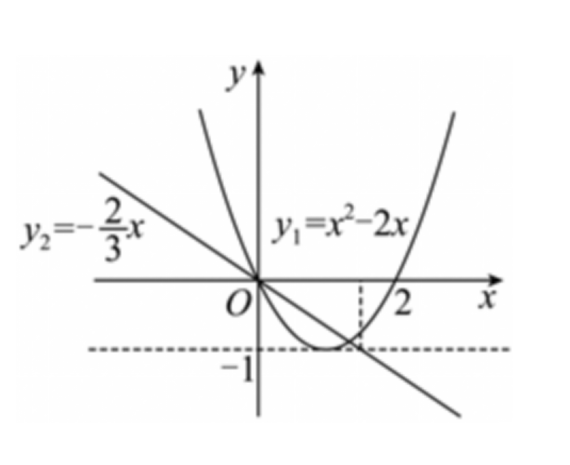
\includegraphics[width=0.24\textwidth]{figures/gao102_q7.png}
\end{center}
\step{当 $m>\dfrac32$ 时，当 $x>m$ 时 $f(x)\in\left(-\infty,-\dfrac23m\right)$，当 $x\leqslant m$ 时 $f(x)\in[-1,+\infty)$，}
\step{显然 $-\dfrac23m<-1$，此时函数 $f(x)$ 的值域不为 $R$，不符合题意；}
\step{当 $m<0$ 时，当 $x>m$ 时，$f(x)\in\left(-\infty,-\dfrac23m\right)$，}
\step{当 $x\leqslant m$ 时，$f(x)\in[m^2-2m,+\infty)$，}
\step{此时 $m^2-2m-\left(-\dfrac23m\right)=m^2-\dfrac43m=m\left(m-\dfrac43\right)>0$，即 $m^2-2m>-\dfrac23m$，}
\step{此时函数 $f(x)$ 的值域不为 $R$，不符合题意；}
\step{当 $0\leqslant m\leqslant\dfrac43$ 时，在 $x\in(0,m)$ 时 $y_2>y_1$，即 $m^2-2m<-\dfrac23m$，}
\step{此时 $f(x)$ 的值域为 $R$，符合题意，}
\step{当 $\dfrac43<m\leqslant\dfrac32$ 时，当 $x>m$ 时，$f(x)\in\left(-\infty,-\dfrac23m\right)$，}
\step{当 $x\leqslant m$ 时，$f(x)\in[-1,+\infty)$，}
\step{此时 $-1-\left(-\dfrac23m\right)=\dfrac23m-1\leqslant0$，即 $-1\leqslant-\dfrac23m$，}
\step{此时函数 $f(x)$ 的值域为 $R$，符合题意；}
\step{综上，$0\leqslant m\leqslant\dfrac32$，即实数 $m$ 的取值范围是 $\left[0,\dfrac32\right]$.}
\solend

\fi

\item 已知函数 $f(x)=x^2-2ax+b$（$a>1$）的定义域和值域都为 $[1,a]$，则 $b=$\blankline[4.4em].

\ifanswer
\solbegin
\step{$f(x)=x^2-2ax+b$（$a>1$）在 $[1,a]$ 严格减，}
\step{则 $f(1)=1-2a+b=a,f(a)=-a^2+b=1$，解得 $a=2,b=5$，所以 $b=5$.}
\solend

\fi

\item 若 $f(x)$ 满足 $f(x+y)=f(x)f(y)$，当 $x>0$ 时，$f(x)$ 的值域为 $(1,+\infty)$，则 $x<0$ 时，
$f(x)$ 的取值范围为\blankline[4.4em].

\ifanswer
\solbegin
\step{因为 $f(x+y)=f(x)f(y)$，令 $x=1$，$y=0$，得 $f(1+0)=f(1)f(0)$，}
\step{又因为当 $x>0$ 时，$f(x)>1$，所以 $f(1)>1>0$，故 $f(0)=1$.}
\step{当 $x<0$ 时，$-x>0$，令 $y=-x$，得 $f(x-x)=f(0)=1=f(x)f(-x)$，}
\step{故 $f(x)=\dfrac1{f(-x)}\in(0,1)$，故 $x<0$ 时，$f(x)$ 的取值范围为 $(0,1)$.}
\solend

\fi

\item 设函数 $f(x)=\begin{cases}x^2+x, & x<0\\ -x^2, & x\geqslant0\end{cases}$，若 $f(f(a))\leqslant2$，则实数 $a$ 的取值范围是\blankline[4.4em].

\ifanswer
\solbegin
\step{函数 $f(x)=\begin{cases}x^2+x, & x<0\\ -x^2, & x\geqslant0\end{cases}$，它的图象如图所示：}
\begin{center}
% 原图第 4 页解析插图直接裁取（原卷排于解析行右侧）。
% 裁框取图形区域，已去粉色水印转灰度。
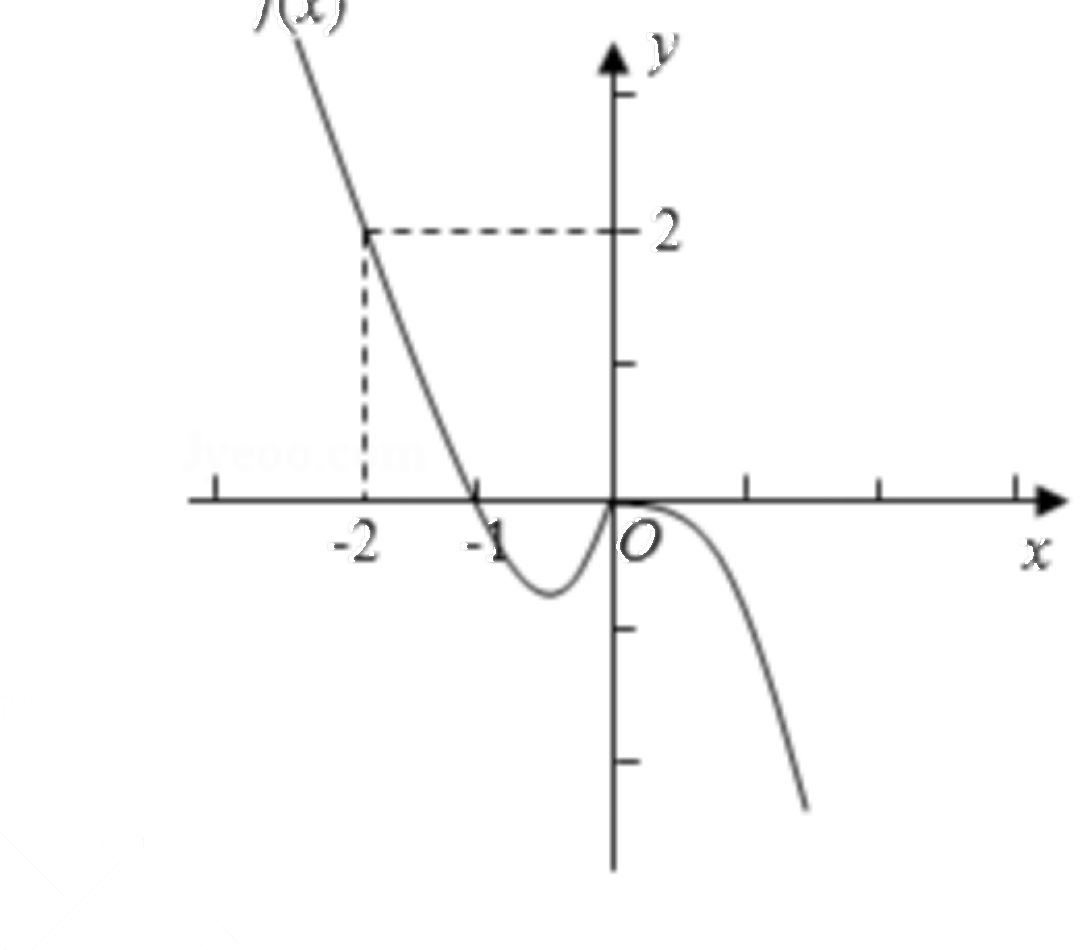
\includegraphics[width=0.30\textwidth]{figures/gao102_q10.png}
\end{center}
\step{由 $f(f(a))\leqslant2$，得 $f(a)\geqslant-2$.}
\step{当 $a<0$ 时，$f(a)=a^2+a=\left(a+\dfrac12\right)^2-\dfrac14\geqslant-2$ 恒成立；}
\step{当 $a\geqslant0$ 时，$f(a)=-a^2\geqslant-2$，即 $a^2\leqslant2$，解得 $0\leqslant a\leqslant\sqrt2$，}
\step{则实数 $a$ 的取值范围是 $(-\infty,\sqrt2]$.}
\solend

\fi

\item 已知二次函数 $f(x)$、$g(x)$ 的二次项系数均为 1，且满足
$\dfrac{f(2025)}{g(2025)}=\dfrac{f(2026)}{g(2026)}=\dfrac{2026}{2025}$，
则 $2026g(2027)-2025f(2027)$ 的值为\blankline[4.4em].

\ifanswer
\solbegin
\step{令 $h(x)=2026g(x)-2025f(x)$，其二次项系数为 $2026-2025=1$.}
\step{由比例条件得 $h(2025)=h(2026)=0$，}
\step{因此 $h(x)=(x-2025)(x-2026),h(2027)=2\times1=2$.}
\solend

\fi

\item 已知函数 $f(x)=\left\lvert x+\dfrac1x-a\right\rvert+1$，对任意实数 $x_1$、$x_2$、$x_3\in\left[\dfrac13,3\right]$，使得以
$f(x_1)$、$f(x_2)$、$f(x_3)$ 数值为边长可构成三角形，则实数 $a$ 的取值范围为\blankline[4.4em].

\ifanswer
\solbegin
\step{对任意实数 $x_1,x_2,x_3\in\left[\dfrac13,3\right]$，}
\step{使得以 $f(x_1)$、$f(x_2)$、$f(x_3)$ 数值为边长可构成三角形，}
\step{只需 $2f(x)_{\min}>f(x)_{\max}$，设 $g(x)=x+\dfrac1x-a$，}
\step{当 $x\in\left[\dfrac13,1\right)$ 时，函数 $g(x)$ 严格减，当 $x\in(1,3]$ 时，函数 $g(x)$ 严格增，}
\step{因为 $g(1)=2-a,g(3)=\dfrac{10}3-a,g\left(\dfrac13\right)=\dfrac{10}3-a$，所以 $g(x)\in\left[2-a,\dfrac{10}3-a\right]$，}
\step{当 $2-a\geqslant0$ 时，即 $a\leqslant2$ 时，$f(x)=\left\lvert x+\dfrac1x-a\right\rvert+1=g(x)+1$，}
\step{此时 $f(x)\in\left[3-a,\dfrac{13}3-a\right]$，}
\step{因此由 $2f(x)_{\min}>f(x)_{\max}\Rightarrow2(3-a)>\dfrac{13}3-a\Rightarrow a<\dfrac53$，而 $a\leqslant2$，所以 $a<\dfrac53$；}
\step{当 $\dfrac{10}3-a\leqslant0$，即 $a\geqslant\dfrac{10}3$ 时，$f(x)=\left\lvert x+\dfrac1x-a\right\rvert+1=-g(x)+1$，}
\step{此时 $f(x)\in\left[a-\dfrac73,a-1\right]$，}
\step{因此由 $2f(x)_{\min}>f(x)_{\max}\Rightarrow2\left(a-\dfrac73\right)>a-1\Rightarrow a>\dfrac{11}3$，而 $a\geqslant\dfrac{10}3$，所以 $a>\dfrac{11}3$，}
\step{若 $2-a<0<\dfrac{10}3-a$ 时，即 $2<a<\dfrac{10}3$ 时，}
\step{若 $a-2\geqslant\dfrac{10}3-a\Rightarrow a\geqslant\dfrac83$，即当 $\dfrac83\leqslant a<\dfrac{10}3$ 时，}
\step{显然此时 $f(x)_{\min}=1$，$f(x)_{\max}=a-2+1=a-1$，}
\step{由 $2f(x)_{\min}>f(x)_{\max}\Rightarrow2\times1>a-1\Rightarrow a<3$，显然 $\dfrac83\leqslant a<3$，}
\step{若 $a-2<\dfrac{10}3-a\Rightarrow a<\dfrac83$，即当 $2<a<\dfrac83$ 时，}
\step{显然此时 $f(x)_{\min}=1,f(x)_{\max}=\dfrac{10}3-a+1=\dfrac{13}3-a$，}
\step{因此由 $2f(x)_{\min}>f(x)_{\max}\Rightarrow2\times1>\dfrac{13}3-a\Rightarrow a>\dfrac73$，而 $\dfrac73<a<\dfrac83$，}
\step{综上，实数 $a$ 的取值范围为 $\left(-\infty,\dfrac53\right)\cup\left(\dfrac73,3\right)\cup\left(\dfrac{11}3,+\infty\right)$.}
\solend

\fi

\end{enumerate}

\bigsec{二、选择题}

\begin{enumerate}
\setcounter{enumi}{12}

\item 已知 $f(x)$ 是定义在 $\R$ 上的奇函数，$g(x)$ 是定义在 $\R$ 上的偶函数，则\mbox{（\quad）}

\keepwithprev
A. $f(x)g(x)$ 是偶函数\qquad B. $f(g(x))$ 是奇函数

C. $f(x)-g(x)$ 是奇函数\qquad D. $g(f(x))$ 是偶函数

\ifanswer
\solbegin
\step{$g(f(x))$ 的定义域为 $\R$，且 $g(f(-x))=g(-f(x))=g(f(x))$，}
\step{所以 $g(f(x))$ 是偶函数，故选 $D$.}
\solend

\fi

\item 已知定义在 $R$ 上的偶函数 $f(x)=\lvert x-m+1\rvert-2$，若正实数 $a$、$b$ 满足 $f(a)+f(2b)=m$，
则 $\dfrac1a+\dfrac2b$ 的最小值为\mbox{（\quad）}

\keepwithprev
A. $\dfrac95$\qquad\qquad B. $9$\qquad\qquad C. $\dfrac85$\qquad\qquad D. $8$

\ifanswer
\solbegin
\step{因为 $f(x)=\lvert x-m+1\rvert-2$ 是偶函数，所以 $-m+1=0$，所以 $m=1$，}
\step{所以 $f(x)=\lvert x\rvert-2$，若正实数 $a$、$b$ 满足 $f(a)+f(2b)=m$，}
\step{则 $a-2+2b-2=1$，所以 $a+2b=5$，}
\step{所以 $\dfrac1a+\dfrac2b=\dfrac15(a+2b)\left(\dfrac1a+\dfrac2b\right)=\dfrac15\left(5+\dfrac{2a}b+\dfrac{2b}a\right)\geqslant\dfrac95$，}
\step{当且仅当 $a=b=\dfrac53$ 时取等号，则 $\dfrac1a+\dfrac2b$ 的最小值为 $\dfrac95$，故选 $A$.}
\solend

\fi

\item 设函数 $g(x)=x^2-2$（$x\in\R$），$f(x)=\begin{cases}g(x)+x+4, & x<g(x)\\ g(x)-x, & x\geqslant g(x)\end{cases}$，则 $f(x)$ 的值域是

\mbox{（\quad）}

\keepwithprev
A. $\left[-\dfrac94,0\right]\cup(1,+\infty)$\qquad\qquad B. $[0,+\infty)$

C. $\left[-\dfrac94,+\infty\right)$\qquad\qquad D. $\left[-\dfrac94,0\right]\cup(2,+\infty)$

\ifanswer
\solbegin
\step{当 $x<g(x)$，即 $x<x^2-2$，$(x-2)(x+1)>0$ 时，$x>2$ 或 $x<-1$，}
\step{$f(x)=g(x)+x+4=x^2-2+x+4=x^2+x+2=(x+0.5)^2+1.75$，}
\step{其最小值趋向于 $f(-1)$ 即 2，无最大值，}
\step{因此这个区间的值域为 $(2,+\infty)$.}
\step{当 $x\geqslant g(x)$ 时，$-1\leqslant x\leqslant2$，$f(x)=g(x)-x=x^2-2-x=(x-0.5)^2-2.25$，}
\step{其最小值为 $f(0.5)=-2.25$，其最大值为 $f(2)=0$，}
\step{因此这区间的值域为 $[-2.25,0]$.}
\step{综上，函数值域为 $\left[-\dfrac94,0\right]\cup(2,+\infty)$，故选 $D$.}
\solend

\fi

\item 设 $D$ 是含数 1 的有限实数集，$f(x)$ 是定义在 $D$ 上的函数，若 $f(x)$ 的图象绕原点逆时针
旋转 $\dfrac{\pi}{6}$ 与原图象重合，则在以下各项中，$f(1)$ 的可能取值只能是\mbox{（\quad）}

\keepwithprev
A. $\sqrt3$\qquad\qquad B. $\dfrac{\sqrt3}2$\qquad\qquad C. $\dfrac{\sqrt3}3$\qquad\qquad D. $0$

\ifanswer
\solbegin
\step{问题相当于圆上由 12 个点为一组，每次绕原点逆时针旋转 $\dfrac{\pi}{6}$ 个单位后与下一个点}
\step{会重合。我们可以通过代入和赋值的方法，当 $f(1)=\sqrt3$、$\dfrac{\sqrt3}3$、$0$ 时，}
\step{此时得到的圆心角为 $\dfrac{\pi}{3}$、$\dfrac{\pi}{6}$、$0$，然而此时 $x=0$ 或者 $x=1$ 时，}
\step{都有 2 个 $y$ 与之对应，而我们知道函数的定义就是要求一个 $x$ 只能对应一个 $y$，}
\step{因此只有当 $x=\dfrac{\sqrt3}2$，此时旋转 $\dfrac{\pi}{6}$，此时满足一个 $x$ 只会对应一个 $y$，故选 $B$.}
\solend

\fi

\end{enumerate}

\bigsec{三、解答题}

\begin{enumerate}
\setcounter{enumi}{16}

\item 求下列函数的值域.

（1）$y=\dfrac{2x^2-3x+5}{x-1}\left(x\in\left[\dfrac32,3\right]\right)$；

（2）$f(x)=\sqrt{x}-\sqrt{2-x}+\sqrt{x(2-x)}$.

\ansspace*[10]

\ifanswer
\solbegin
\stepm{（1）}{令 $t=x-1$，则 $t\in\left[\dfrac12,2\right]$，原函数化为 $Y(t)=2t+\dfrac4t+1$.}
\step{当 $0<u<v$ 时，$Y(v)-Y(u)=2(v-u)\left(1-\dfrac2{uv}\right)$，}
\step{所以 $Y$ 在 $\left[\dfrac12,\sqrt2\right]$ 上严格递减，在 $[\sqrt2,2]$ 上严格递增.}
\step{由 $Y(\sqrt2)=4\sqrt2+1,Y\left(\dfrac12\right)=10,Y(2)=7$，得值域为 $[4\sqrt2+1,10]$.}
\stepm{（2）}{定义域为 $[0,2]$.}
\step{令 $s=\sqrt{x}-\sqrt{2-x}$，$\sqrt{x}$ 与 $-\sqrt{2-x}$ 均随 $x$ 严格递增，}
\step{$s$ 从 $-\sqrt2$ 递增到 $\sqrt2$，即 $s\in[-\sqrt2,\sqrt2]$.}
\step{由 $s^2=2-2\sqrt{x(2-x)}$，得 $f(x)=s+\dfrac{2-s^2}2=-\dfrac12(s-1)^2+\dfrac32$.}
\step{当 $s=1$ 时取得最大值 $\dfrac32$；当 $s=-\sqrt2$ 时取得最小值 $-\sqrt2$；}
\step{因此值域为 $\left[-\sqrt2,\dfrac32\right]$.}
\solend

\fi

\item 已知 $f(2x+1)=\dfrac{2x+1}{x+1}$.

（1）解不等式 $f(x)<x$；

（2）求 $f(1)+f(2)+\cdots+f(6)+f\left(\dfrac12\right)+f\left(\dfrac13\right)+\cdots+f\left(\dfrac16\right)$ 的值.

\ansspace*[12]

\ifanswer
\solbegin
\step{令 $t=2x+1$，则 $x=\dfrac{t-1}2$，得 $f(t)=\dfrac{2t}{t+1},t\neq-1$.}
\stepm{（1）}{不等式等价于 $\dfrac{2x}{x+1}<x\Leftrightarrow\dfrac{x(x-1)}{x+1}>0$.}
\step{以 $-1,0,1$ 分区间判断符号，得解集为 $(-1,0)\cup(1,+\infty)$.}
\stepm{（2）}{当 $x>0$ 时，$f(x)+f\left(\dfrac1x\right)=\dfrac{2x}{x+1}+\dfrac2{x+1}=2$.}
\step{将 $f(2),\cdots,f(6)$ 分别与其倒数对应的函数值配对，共 5 对，且 $f(1)=1$，}
\step{因此原式$=1+5\times2=11$.}
\solend

\fi

\item 已知函数 $f(x)$、$g(x)$ 是定义在 $R$ 上的函数，其中 $f(x)$ 是奇函数，$g(x)$ 是偶函数，且
$f(x)+g(x)=ax^2-x$.

（1）求 $f(x)$ 和 $g(x)$ 的解析式；

（2）$h(x)=f(x)+g(x)+(1-a)x^2-2ax+4$ 在 $[1,3]$ 上有两个零点，求实数 $a$ 的取值范
围.

\ansspace*[14]

\ifanswer
\solbegin
\stepm{（1）}{因为 $f(x)+g(x)=ax^2-x$①，所以 $f(-x)+g(-x)=ax^2+x$，}
\step{又 $f(x)$ 是奇函数，$g(x)$ 是偶函数，}
\step{所以 $f(-x)=-f(x)$，$g(-x)=g(x)$，}
\step{所以 $-f(x)+g(x)=ax^2+x$②，}
\step{联立①②解得 $f(x)=-x$，$g(x)=ax^2$.}
\stepm{（2）}{$h(x)=f(x)+g(x)+(1-a)x^2-2ax+4$}
\step{$=ax^2-x+(1-a)x^2-2ax+4=x^2-(2a+1)x+4$，}
\step{是开口向上，对称轴为 $x=\dfrac{2a+1}2$ 的二次函数，}
\step{因为 $h(x)$ 在 $[1,3]$ 上有两个零点，所以 $\begin{cases}\Delta=(2a+1)^2-16>0\\ 1<\dfrac{2a+1}2<3\\ h(1)=1-(2a+1)+4\geqslant0\\ h(3)=9-3(2a+1)+4\geqslant0\end{cases}$，}
\step{解得 $\dfrac32<a\leqslant\dfrac53$，故实数 $a$ 的取值范围为 $\left(\dfrac32,\dfrac53\right]$.}
\solend

\fi

\item 若函数 $f(x)$ 在区间 $[a,b]$ 上的值域恰为 $\left[\dfrac1b,\dfrac1a\right]$，则称区间 $[a,b]$ 为 $f(x)$ 的一个“倒域
区间”。已知定义在 $[-4,4]$ 上的奇函数 $g(x)$，当 $x\in[0,4]$ 时，$g(x)=-x^2+2x$.

（1）求 $g(x)$ 的解析式；

（2）若关于 $x$ 的方程 $g(x)=-mx-m$ 在 $(0,4)$ 上恰有两个不相等的实数根，求实数 $m$ 的
取值范围；

（3）求函数 $g(x)$ 在 $[-4,0]$ 内的“倒域区间”.

\ansspace*[16]

\ifanswer
\solbegin
\stepm{（1）}{当 $x\in[-4,0)$ 时，$-x\in(0,4]$，}
\step{由奇函数的定义得 $g(x)=-g(-x)=-[(-x)^2+2(-x)]=x^2+2x$，}
\step{所以 $g(x)=\begin{cases}-x^2+2x, & 0\leqslant x\leqslant4\\ x^2+2x, & -4\leqslant x<0\end{cases}$.}
\stepm{（2）}{方程 $g(x)=-mx-m$，即 $x^2-(m+2)x-m=0$，}
\step{设 $h(x)=x^2-(m+2)x-m$，$0<x<4$，}
\step{由题意得 $\begin{cases}h(0)=-m>0\\ h(4)=8-5m>0\\ \Delta=(m+2)^2+4m>0\\ 0<\dfrac{m+2}2<4\end{cases}$，解得 $2\sqrt3-4<m<0$，}
\step{即实数 $m$ 的取值范围是 $(2\sqrt3-4,0)$.}
\stepm{（3）}{易得当 $-4\leqslant a<b<0$ 时，$\dfrac1b<\dfrac1a$，}
\step{且 $g(x)$ 在 $[-4,-1]$ 上严格减，在 $[-1,0]$ 上严格增，}
\step{故当 $x\in[-4,0]$ 时，$g(x)_{\min}=g(-1)=-1$，}
\step{所以 $\dfrac1b\geqslant-1$，所以 $-4<b\leqslant-1$，所以 $-4\leqslant a<b\leqslant-1$，}
\step{则 $\begin{cases}g(a)=a^2+2a=\dfrac1a\\ g(b)=b^2+2b=\dfrac1b\\ -4\leqslant a<b\leqslant-1\end{cases}$，解得 $\begin{cases}a=-\dfrac{1+\sqrt5}2\\ b=-1\end{cases}$，}
\step{所以 $g(x)$ 在 $[-4,0]$ 内的“倒域区间”为 $\left[-\dfrac{1+\sqrt5}2,-1\right]$.}
\solend

\fi

\item 我们知道：函数 $y=f(x)$ 的图象关于坐标原点成中心对称图形的充要条件是函数
$y=f(x)$ 为奇函数。有同学发现可以推广为：函数 $y=f(x)$ 的图象关于点 $(a,b)$ 成中心对
称图形的充要条件为函数 $y=f(x+a)-b$ 为奇函数。已知函数 $f(x)=\dfrac{2x}{3-x}$.

（1）求函数 $f(x)$ 图象的对称中心；

（2）若定义在 $R$ 上的函数 $y=g(x)$ 的图象关于点 $(1,2)$ 对称，且 $g(1)=2$，当 $x\in[0,1)$
时，$g(x)=x^2-tx+t+1$.

（$i$）求 $g(-3)+g(5)$ 的值；

（$ii$）若对$\forall x_1\in[0,2]$，$\exists x_2\in[-3,2]$ 使得 $g(x_1)=f(x_2)$ 恒成立，求实数 $t$ 的取值范围.

\ansspace*[18]

\ifanswer
\solbegin
\stepm{（1）}{由 $f(x)=\dfrac{2x}{3-x}=-2+\dfrac6{3-x}$，}
\step{易得 $f(x+3)+2=-2+\dfrac6{3-(x+3)}+2=-\dfrac6x$ 为奇函数，}
\step{$f(x)$ 的图象关于 $(3,-2)$ 对称.}
\stepm{（2）}{（$i$）$y=g(x)$ 图象关于点 $(1,2)$ 对称，则 $g(1+x)+g(1-x)=4$，}
\step{令 $x=4$，则 $g(-3)+g(5)=4$.}
\step{（$ii$）有 $g(x)$ 在 $x\in[0,2]$ 的取值范围为 $f(x)$ 在 $x\in[-3,2]$ 的取值范围的}
\step{子集，}
\step{因为 $f(x)=\dfrac{2x}{3-x}=\dfrac{6-2(3-x)}{3-x}=\dfrac6{3-x}-2$ 在 $[-3,2]$ 上严格增，}
\step{所以 $f(x)$ 在 $x\in[-3,2]$ 上的取值范围为 $[-1,4]$，}
\step{记 $g(x)$ 的值域为 $A$，且 $g(1)=2$，当 $x\in[0,1)$ 时 $g(x)=x^2-tx+t+1$，}
\step{①当 $\dfrac t2\leqslant0$，即 $t\leqslant0$ 时，有 $g(x)$ 在 $[0,1)$ 上严格增，}
\step{由对称性得 $g(x)$ 在 $[1,2]$ 上严格增，故 $g(x)$ 在 $[0,2]$ 上严格增，}
\step{故 $g(x)_{\min}=g(0)=t+1$，$g(x)_{\max}=g(2)=4-(t+1)=3-t$，$t\leqslant0$，}
\step{则 $A=[t+1,3-t]\subseteq[-1,4]$，即 $\begin{cases}t\leqslant0\\ t+1\geqslant-1\\ 3-t\leqslant4\end{cases}$，解得 $-1\leqslant t\leqslant0$.}
\step{②当 $0<\dfrac t2<1$，即 $0<t<2$ 时，}
\step{$g(x)$ 在 $\left(0,\dfrac t2\right)$ 上严格减，在 $\left(\dfrac t2,1\right)$ 上严格增，}
\step{由对称性得 $g(x)$ 在 $\left(2-\dfrac t2,2\right)$ 上严格减，在 $\left(1,2-\dfrac t2\right)$ 上严格增，}
\step{故 $g(x)$ 在 $\left(0,\dfrac t2\right)$ 上严格减，在 $\left(\dfrac t2,2-\dfrac t2\right)$ 上严格增，}
\step{在 $\left(2-\dfrac t2,2\right)$ 上严格减，则 $A=\left[g\left(\dfrac t2\right),g\left(2-\dfrac t2\right)\right]$，}
\step{由 $0<t<2$，得 $g(0)=t+1\in(1,3)$，$g(2)=4-(t+1)=3-t\in(1,3)$，}
\step{$g\left(\dfrac t2\right)=-\dfrac{t^2}4+t+1=-\dfrac14(t-2)^2+2\in(1,2]$，}
\step{又 $g\left(\dfrac t2\right)+g\left(2-\dfrac t2\right)=4$，$g\left(2-\dfrac t2\right)\in(2,3)$，}
\step{当 $0<t<2$ 时，$A\subseteq[-1,4]$ 恒成立，}
\step{③当 $\dfrac t2\geqslant1$，即 $t\geqslant2$ 时，有 $g(x)$ 在 $[0,1)$ 上严格减，}
\step{由对称点 $(1,2)$ 得 $g(x)$ 在 $[1,2]$ 上严格减，所以 $g(x)$ 在 $[0,2]$ 上严格减，}
\step{故 $g(x)_{\max}=g(0)=t+1$，$g(x)_{\min}=g(2)=4-(t+1)=3-t$，$t\geqslant2$，}
\step{则 $A=[3-t,t+1]\subseteq[-1,4]$，即 $\begin{cases}t\geqslant2\\ t+1\leqslant4\\ 3-t\geqslant-1\end{cases}$，解得 $2\leqslant t\leqslant3$.}
\step{综上，$t$ 的范围为 $\{t\mid-1\leqslant t\leqslant3\}$.}
\solend

\fi

\end{enumerate}

\end{document}
"
%
% 原始材料：微信公众号“魔都数学加油站”文章，作者破晓，2026-11-01 21:56 发布；
% 连载“27学年高一102”，原文标题“27学年高一102——2026-2027年上海市华师大二附中高一上周末作业5函数”；
% 原文链接：https://mp.weixin.qq.com/s/CDvOCcxFskIe9aFUeKi3Ww。
% 正文为 13 张 PNG 页（第 1、2、10、13 页 2560×3620，其余 4762×6735），题目下印有【解析】，为讲评版。
% 题目、解析均据原图转录；卷面水印及公众号页脚未录入。
%
% 卷首标题：原卷印作“2026-2027 年华师大二附中高一上周末作业 5”（公众号标题中的“上海市”“函数”
% 卷面标题行没有，本稿照卷面），年份区间按全稿惯例排 en dash；原卷未印副标题，本稿按题目内容
% 标为“函数”（全稿首份以函数为单一模块的卷子）。
%
% 与原卷的排版差异：
%   ① 原文从第 3 题起，填空题编号为 3—12、选择题为 13—16、解答题为 17—21，本稿保留原题号；
%   ② 原卷每题下直接印【解析】，本稿按全稿惯例将解析置于答案版；选择题括号内未印答案，另由
%      解析末句“故选 X”给出；
%   ③ 原卷未印副标题，本稿按“知识模块”口径补出；
%   ④ 原卷填空横线按全稿惯例排为 \blankline[4.4em]；解答题按惯例加 \ansspace；选择题括号排
%      \mbox{（\quad）}、选项段前按惯例加 \keepwithprev；
%   ⑤ 原卷 $f(x)_{min}$、$f(x)_{max}$ 等下标排斜体，按 高一96 成例改正体 $\min$、$\max$；
%   ⑥ 原卷数集排斜体 $R$（第 13 题排粗体），按全稿惯例改 $\R$；
%   ⑦ 第 7、10 两题的解析插图裁自原图（去粉色水印转灰度），仅答案版显示。
%
% 原卷存疑／笔误（均照录加注）：
%   第 3 题解析“减去都对应 −2 和 2 的”措辞含糊（意为减去恒取 −2 与恒取 2 的两个常函数）；
%   第 15 题解析“其最小值趋向于 f(−1) 即 2”（该段 f(x)=x²+x+2 在 x→−1⁻ 时趋于 2、取不到）；
%   第 16 题解析末句“因此只有当 x=√3/2”（按上下文应为 f(1)=√3/2）；
%   第 16 题解析以 f(1)=√3、√3/3、0 赋值时称“得到的圆心角为 π/3、π/6、0”，其中 √3/3 对应
%   圆心角 π/6 的说法与该点 (1,√3/3) 的实际幅角一致，但与选项 C（√3/3）被排除的结论矛盾
%   （幅角 π/6 的点旋转 π/6 后落到幅角 π/3 处，仍占 12 等分点位，原卷解析未展开），照录。
%
% 行数核对：逐题数 \step/\stepm 条数，合计 155 条（Q3：2；Q4：3；Q5：6；Q6：5；Q7：19；
% Q8：2；Q9：4；Q10：5；Q11：3；Q12：19；Q13：2；Q14：5；Q15：8；Q16：5；Q17：10；
% Q18：6；Q19：10；Q20：13；Q21：28），与原卷印刷行逐题相等。
%
\documentclass[a4paper,11pt]{article}
\usepackage{common}

\begin{document}

\examtitlest[3]{2026--2027 年华师大二附中高一上周末作业 5}{函数}

\bigsec{一、填空题}

\begin{enumerate}
\setcounter{enumi}{2}

\item 已知函数 $y=f(x)$ 的定义域为 $\{-2,-1,1,2\}$，值域为 $\{-2,2\}$，则满足条件的函数
$y=f(x)$ 最多有\blankline[4.4em]个.

\ifanswer
\solbegin
\step{定义域中 4 个元素每个都可以对应 $-2$ 和 $2$ 中的一个，减去都对应 $-2$ 和 $2$ 的，}
\step{则满足条件的函数 $y=f(x)$ 最多有 $2^4-2=14$.}
\solend

\fi

\item 已知函数 $f(2x)$ 的定义域为 $[-2,2]$，则函数 $f(x-3)$ 的定义域为\blankline[4.4em].

\ifanswer
\solbegin
\step{因为函数 $f(2x)$ 的定义域为 $[-2,2]$，即 $-2\leqslant x\leqslant2$，所以 $-4\leqslant2x\leqslant4$，}
\step{得 $f(x)$ 的定义域为 $[-4,4]$，由 $-4\leqslant x-3\leqslant4$，解得 $-1\leqslant x\leqslant7$，}
\step{即函数 $f(x-3)$ 的定义域为 $[-1,7]$.}
\solend

\fi

\item 函数 $f(x)=\begin{cases}-x-1, & x<0\\ -x+1, & x>0\end{cases}$，则 $f(x)-f(-x)>1$ 的解集为\blankline[4.4em].

\ifanswer
\solbegin
\step{定义域为 $\{x\mid x\neq0\}$.}
\step{当 $x<0$ 时，$-x>0,f(-x)=x+1$，}
\step{$f(x)-f(-x)=(-x-1)-(x+1)=-2x-2>1$，得 $x<-\dfrac32$.}
\step{当 $x>0$ 时，$f(-x)=x-1,f(x)-f(-x)=(-x+1)-(x-1)=-2x+2>1$，}
\step{得 $0<x<\dfrac12$.}
\step{故解集为 $\left(-\infty,-\dfrac32\right)\cup\left(0,\dfrac12\right)$.}
\solend

\fi

\item 已知函数 $f(x)=x^2-2(m-3)x+5$ 在区间 $[2,+\infty)$ 上的最小值为 1，则实数 $m=$\blankline[4.4em].

\ifanswer
\solbegin
\step{函数 $f(x)$ 图象的对称轴为 $x=m-3$.}
\step{当 $m-3\leqslant2$，即 $m\leqslant5$ 时，$f(x)_{\min}=f(2)=9-4m+12=1$，解得 $m=5$；}
\step{当 $m-3>2$，即 $m>5$ 时，$f(x)_{\min}=f(m-3)=-m^2+6m-4=1$，}
\step{解得 $m=5$（舍去）或 $1$（舍去），}
\step{综上，$m=5$.}
\solend

\fi

\item 已知函数 $f(x)=\begin{cases}x^2-2x, & x\leqslant m\\ -\dfrac23x, & x>m\end{cases}$ 的值域为 $R$，则实数 $m$ 的取值范围是\blankline[4.4em].

\ifanswer
\solbegin
\step{对于函数 $y_1=x^2-2x$，则 $y_1=(x-1)^2-1\geqslant-1$，当且仅当 $x=1$ 时取等号，}
\step{且函数在 $(-\infty,1)$ 上严格减，在 $(1,+\infty)$ 上严格增，}
\step{对于函数 $y_2=-\dfrac23x$，令 $y_2=-1$，则 $x=\dfrac32$，且函数在定义域上严格减，}
\step{令 $x^2-2x=-\dfrac23x$，解得 $x=0$ 或 $x=\dfrac43$，}
\step{所以 $y_2=-\dfrac23x$ 与 $y_1=x^2-2x$ 的两个交点分别为 $(0,0)$、$\left(\dfrac43,-\dfrac89\right)$，}
\step{则函数 $y_2=-\dfrac23x$ 与 $y_1=x^2-2x$ 的图象如图所示：}
\begin{center}
% 原图第 2 页解析插图直接裁取（原卷排于解析行右侧）。
% 裁框取图形区域，已去粉色水印转灰度。
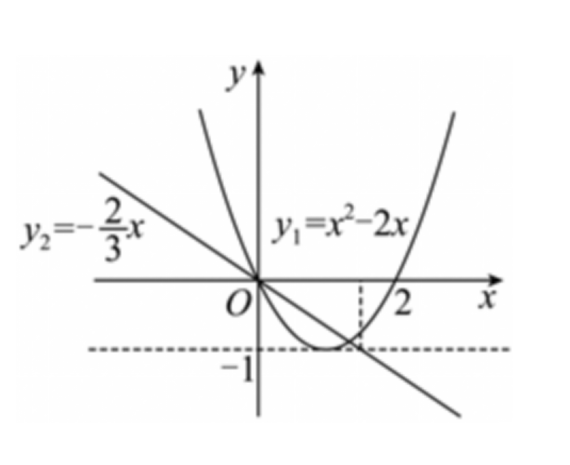
\includegraphics[width=0.24\textwidth]{figures/gao102_q7.png}
\end{center}
\step{当 $m>\dfrac32$ 时，当 $x>m$ 时 $f(x)\in\left(-\infty,-\dfrac23m\right)$，当 $x\leqslant m$ 时 $f(x)\in[-1,+\infty)$，}
\step{显然 $-\dfrac23m<-1$，此时函数 $f(x)$ 的值域不为 $R$，不符合题意；}
\step{当 $m<0$ 时，当 $x>m$ 时，$f(x)\in\left(-\infty,-\dfrac23m\right)$，}
\step{当 $x\leqslant m$ 时，$f(x)\in[m^2-2m,+\infty)$，}
\step{此时 $m^2-2m-\left(-\dfrac23m\right)=m^2-\dfrac43m=m\left(m-\dfrac43\right)>0$，即 $m^2-2m>-\dfrac23m$，}
\step{此时函数 $f(x)$ 的值域不为 $R$，不符合题意；}
\step{当 $0\leqslant m\leqslant\dfrac43$ 时，在 $x\in(0,m)$ 时 $y_2>y_1$，即 $m^2-2m<-\dfrac23m$，}
\step{此时 $f(x)$ 的值域为 $R$，符合题意，}
\step{当 $\dfrac43<m\leqslant\dfrac32$ 时，当 $x>m$ 时，$f(x)\in\left(-\infty,-\dfrac23m\right)$，}
\step{当 $x\leqslant m$ 时，$f(x)\in[-1,+\infty)$，}
\step{此时 $-1-\left(-\dfrac23m\right)=\dfrac23m-1\leqslant0$，即 $-1\leqslant-\dfrac23m$，}
\step{此时函数 $f(x)$ 的值域为 $R$，符合题意；}
\step{综上，$0\leqslant m\leqslant\dfrac32$，即实数 $m$ 的取值范围是 $\left[0,\dfrac32\right]$.}
\solend

\fi

\item 已知函数 $f(x)=x^2-2ax+b$（$a>1$）的定义域和值域都为 $[1,a]$，则 $b=$\blankline[4.4em].

\ifanswer
\solbegin
\step{$f(x)=x^2-2ax+b$（$a>1$）在 $[1,a]$ 严格减，}
\step{则 $f(1)=1-2a+b=a,f(a)=-a^2+b=1$，解得 $a=2,b=5$，所以 $b=5$.}
\solend

\fi

\item 若 $f(x)$ 满足 $f(x+y)=f(x)f(y)$，当 $x>0$ 时，$f(x)$ 的值域为 $(1,+\infty)$，则 $x<0$ 时，
$f(x)$ 的取值范围为\blankline[4.4em].

\ifanswer
\solbegin
\step{因为 $f(x+y)=f(x)f(y)$，令 $x=1$，$y=0$，得 $f(1+0)=f(1)f(0)$，}
\step{又因为当 $x>0$ 时，$f(x)>1$，所以 $f(1)>1>0$，故 $f(0)=1$.}
\step{当 $x<0$ 时，$-x>0$，令 $y=-x$，得 $f(x-x)=f(0)=1=f(x)f(-x)$，}
\step{故 $f(x)=\dfrac1{f(-x)}\in(0,1)$，故 $x<0$ 时，$f(x)$ 的取值范围为 $(0,1)$.}
\solend

\fi

\item 设函数 $f(x)=\begin{cases}x^2+x, & x<0\\ -x^2, & x\geqslant0\end{cases}$，若 $f(f(a))\leqslant2$，则实数 $a$ 的取值范围是\blankline[4.4em].

\ifanswer
\solbegin
\step{函数 $f(x)=\begin{cases}x^2+x, & x<0\\ -x^2, & x\geqslant0\end{cases}$，它的图象如图所示：}
\begin{center}
% 原图第 4 页解析插图直接裁取（原卷排于解析行右侧）。
% 裁框取图形区域，已去粉色水印转灰度。
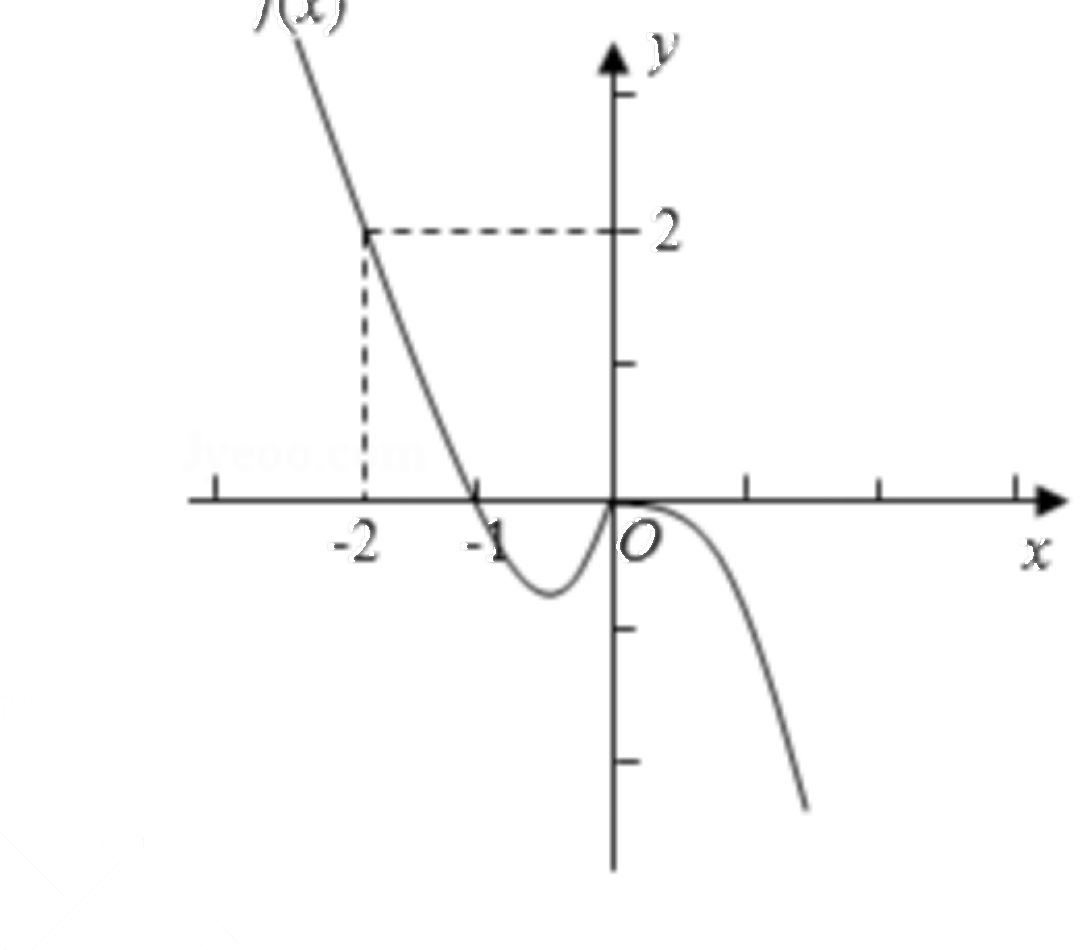
\includegraphics[width=0.30\textwidth]{figures/gao102_q10.png}
\end{center}
\step{由 $f(f(a))\leqslant2$，得 $f(a)\geqslant-2$.}
\step{当 $a<0$ 时，$f(a)=a^2+a=\left(a+\dfrac12\right)^2-\dfrac14\geqslant-2$ 恒成立；}
\step{当 $a\geqslant0$ 时，$f(a)=-a^2\geqslant-2$，即 $a^2\leqslant2$，解得 $0\leqslant a\leqslant\sqrt2$，}
\step{则实数 $a$ 的取值范围是 $(-\infty,\sqrt2]$.}
\solend

\fi

\item 已知二次函数 $f(x)$、$g(x)$ 的二次项系数均为 1，且满足
$\dfrac{f(2025)}{g(2025)}=\dfrac{f(2026)}{g(2026)}=\dfrac{2026}{2025}$，
则 $2026g(2027)-2025f(2027)$ 的值为\blankline[4.4em].

\ifanswer
\solbegin
\step{令 $h(x)=2026g(x)-2025f(x)$，其二次项系数为 $2026-2025=1$.}
\step{由比例条件得 $h(2025)=h(2026)=0$，}
\step{因此 $h(x)=(x-2025)(x-2026),h(2027)=2\times1=2$.}
\solend

\fi

\item 已知函数 $f(x)=\left\lvert x+\dfrac1x-a\right\rvert+1$，对任意实数 $x_1$、$x_2$、$x_3\in\left[\dfrac13,3\right]$，使得以
$f(x_1)$、$f(x_2)$、$f(x_3)$ 数值为边长可构成三角形，则实数 $a$ 的取值范围为\blankline[4.4em].

\ifanswer
\solbegin
\step{对任意实数 $x_1,x_2,x_3\in\left[\dfrac13,3\right]$，}
\step{使得以 $f(x_1)$、$f(x_2)$、$f(x_3)$ 数值为边长可构成三角形，}
\step{只需 $2f(x)_{\min}>f(x)_{\max}$，设 $g(x)=x+\dfrac1x-a$，}
\step{当 $x\in\left[\dfrac13,1\right)$ 时，函数 $g(x)$ 严格减，当 $x\in(1,3]$ 时，函数 $g(x)$ 严格增，}
\step{因为 $g(1)=2-a,g(3)=\dfrac{10}3-a,g\left(\dfrac13\right)=\dfrac{10}3-a$，所以 $g(x)\in\left[2-a,\dfrac{10}3-a\right]$，}
\step{当 $2-a\geqslant0$ 时，即 $a\leqslant2$ 时，$f(x)=\left\lvert x+\dfrac1x-a\right\rvert+1=g(x)+1$，}
\step{此时 $f(x)\in\left[3-a,\dfrac{13}3-a\right]$，}
\step{因此由 $2f(x)_{\min}>f(x)_{\max}\Rightarrow2(3-a)>\dfrac{13}3-a\Rightarrow a<\dfrac53$，而 $a\leqslant2$，所以 $a<\dfrac53$；}
\step{当 $\dfrac{10}3-a\leqslant0$，即 $a\geqslant\dfrac{10}3$ 时，$f(x)=\left\lvert x+\dfrac1x-a\right\rvert+1=-g(x)+1$，}
\step{此时 $f(x)\in\left[a-\dfrac73,a-1\right]$，}
\step{因此由 $2f(x)_{\min}>f(x)_{\max}\Rightarrow2\left(a-\dfrac73\right)>a-1\Rightarrow a>\dfrac{11}3$，而 $a\geqslant\dfrac{10}3$，所以 $a>\dfrac{11}3$，}
\step{若 $2-a<0<\dfrac{10}3-a$ 时，即 $2<a<\dfrac{10}3$ 时，}
\step{若 $a-2\geqslant\dfrac{10}3-a\Rightarrow a\geqslant\dfrac83$，即当 $\dfrac83\leqslant a<\dfrac{10}3$ 时，}
\step{显然此时 $f(x)_{\min}=1$，$f(x)_{\max}=a-2+1=a-1$，}
\step{由 $2f(x)_{\min}>f(x)_{\max}\Rightarrow2\times1>a-1\Rightarrow a<3$，显然 $\dfrac83\leqslant a<3$，}
\step{若 $a-2<\dfrac{10}3-a\Rightarrow a<\dfrac83$，即当 $2<a<\dfrac83$ 时，}
\step{显然此时 $f(x)_{\min}=1,f(x)_{\max}=\dfrac{10}3-a+1=\dfrac{13}3-a$，}
\step{因此由 $2f(x)_{\min}>f(x)_{\max}\Rightarrow2\times1>\dfrac{13}3-a\Rightarrow a>\dfrac73$，而 $\dfrac73<a<\dfrac83$，}
\step{综上，实数 $a$ 的取值范围为 $\left(-\infty,\dfrac53\right)\cup\left(\dfrac73,3\right)\cup\left(\dfrac{11}3,+\infty\right)$.}
\solend

\fi

\end{enumerate}

\bigsec{二、选择题}

\begin{enumerate}
\setcounter{enumi}{12}

\item 已知 $f(x)$ 是定义在 $\R$ 上的奇函数，$g(x)$ 是定义在 $\R$ 上的偶函数，则\mbox{（\quad）}

\keepwithprev
A. $f(x)g(x)$ 是偶函数\qquad B. $f(g(x))$ 是奇函数

C. $f(x)-g(x)$ 是奇函数\qquad D. $g(f(x))$ 是偶函数

\ifanswer
\solbegin
\step{$g(f(x))$ 的定义域为 $\R$，且 $g(f(-x))=g(-f(x))=g(f(x))$，}
\step{所以 $g(f(x))$ 是偶函数，故选 $D$.}
\solend

\fi

\item 已知定义在 $R$ 上的偶函数 $f(x)=\lvert x-m+1\rvert-2$，若正实数 $a$、$b$ 满足 $f(a)+f(2b)=m$，
则 $\dfrac1a+\dfrac2b$ 的最小值为\mbox{（\quad）}

\keepwithprev
A. $\dfrac95$\qquad\qquad B. $9$\qquad\qquad C. $\dfrac85$\qquad\qquad D. $8$

\ifanswer
\solbegin
\step{因为 $f(x)=\lvert x-m+1\rvert-2$ 是偶函数，所以 $-m+1=0$，所以 $m=1$，}
\step{所以 $f(x)=\lvert x\rvert-2$，若正实数 $a$、$b$ 满足 $f(a)+f(2b)=m$，}
\step{则 $a-2+2b-2=1$，所以 $a+2b=5$，}
\step{所以 $\dfrac1a+\dfrac2b=\dfrac15(a+2b)\left(\dfrac1a+\dfrac2b\right)=\dfrac15\left(5+\dfrac{2a}b+\dfrac{2b}a\right)\geqslant\dfrac95$，}
\step{当且仅当 $a=b=\dfrac53$ 时取等号，则 $\dfrac1a+\dfrac2b$ 的最小值为 $\dfrac95$，故选 $A$.}
\solend

\fi

\item 设函数 $g(x)=x^2-2$（$x\in\R$），$f(x)=\begin{cases}g(x)+x+4, & x<g(x)\\ g(x)-x, & x\geqslant g(x)\end{cases}$，则 $f(x)$ 的值域是

\mbox{（\quad）}

\keepwithprev
A. $\left[-\dfrac94,0\right]\cup(1,+\infty)$\qquad\qquad B. $[0,+\infty)$

C. $\left[-\dfrac94,+\infty\right)$\qquad\qquad D. $\left[-\dfrac94,0\right]\cup(2,+\infty)$

\ifanswer
\solbegin
\step{当 $x<g(x)$，即 $x<x^2-2$，$(x-2)(x+1)>0$ 时，$x>2$ 或 $x<-1$，}
\step{$f(x)=g(x)+x+4=x^2-2+x+4=x^2+x+2=(x+0.5)^2+1.75$，}
\step{其最小值趋向于 $f(-1)$ 即 2，无最大值，}
\step{因此这个区间的值域为 $(2,+\infty)$.}
\step{当 $x\geqslant g(x)$ 时，$-1\leqslant x\leqslant2$，$f(x)=g(x)-x=x^2-2-x=(x-0.5)^2-2.25$，}
\step{其最小值为 $f(0.5)=-2.25$，其最大值为 $f(2)=0$，}
\step{因此这区间的值域为 $[-2.25,0]$.}
\step{综上，函数值域为 $\left[-\dfrac94,0\right]\cup(2,+\infty)$，故选 $D$.}
\solend

\fi

\item 设 $D$ 是含数 1 的有限实数集，$f(x)$ 是定义在 $D$ 上的函数，若 $f(x)$ 的图象绕原点逆时针
旋转 $\dfrac{\pi}{6}$ 与原图象重合，则在以下各项中，$f(1)$ 的可能取值只能是\mbox{（\quad）}

\keepwithprev
A. $\sqrt3$\qquad\qquad B. $\dfrac{\sqrt3}2$\qquad\qquad C. $\dfrac{\sqrt3}3$\qquad\qquad D. $0$

\ifanswer
\solbegin
\step{问题相当于圆上由 12 个点为一组，每次绕原点逆时针旋转 $\dfrac{\pi}{6}$ 个单位后与下一个点}
\step{会重合。我们可以通过代入和赋值的方法，当 $f(1)=\sqrt3$、$\dfrac{\sqrt3}3$、$0$ 时，}
\step{此时得到的圆心角为 $\dfrac{\pi}{3}$、$\dfrac{\pi}{6}$、$0$，然而此时 $x=0$ 或者 $x=1$ 时，}
\step{都有 2 个 $y$ 与之对应，而我们知道函数的定义就是要求一个 $x$ 只能对应一个 $y$，}
\step{因此只有当 $x=\dfrac{\sqrt3}2$，此时旋转 $\dfrac{\pi}{6}$，此时满足一个 $x$ 只会对应一个 $y$，故选 $B$.}
\solend

\fi

\end{enumerate}

\bigsec{三、解答题}

\begin{enumerate}
\setcounter{enumi}{16}

\item 求下列函数的值域.

（1）$y=\dfrac{2x^2-3x+5}{x-1}\left(x\in\left[\dfrac32,3\right]\right)$；

（2）$f(x)=\sqrt{x}-\sqrt{2-x}+\sqrt{x(2-x)}$.

\ansspace*[10]

\ifanswer
\solbegin
\stepm{（1）}{令 $t=x-1$，则 $t\in\left[\dfrac12,2\right]$，原函数化为 $Y(t)=2t+\dfrac4t+1$.}
\step{当 $0<u<v$ 时，$Y(v)-Y(u)=2(v-u)\left(1-\dfrac2{uv}\right)$，}
\step{所以 $Y$ 在 $\left[\dfrac12,\sqrt2\right]$ 上严格递减，在 $[\sqrt2,2]$ 上严格递增.}
\step{由 $Y(\sqrt2)=4\sqrt2+1,Y\left(\dfrac12\right)=10,Y(2)=7$，得值域为 $[4\sqrt2+1,10]$.}
\stepm{（2）}{定义域为 $[0,2]$.}
\step{令 $s=\sqrt{x}-\sqrt{2-x}$，$\sqrt{x}$ 与 $-\sqrt{2-x}$ 均随 $x$ 严格递增，}
\step{$s$ 从 $-\sqrt2$ 递增到 $\sqrt2$，即 $s\in[-\sqrt2,\sqrt2]$.}
\step{由 $s^2=2-2\sqrt{x(2-x)}$，得 $f(x)=s+\dfrac{2-s^2}2=-\dfrac12(s-1)^2+\dfrac32$.}
\step{当 $s=1$ 时取得最大值 $\dfrac32$；当 $s=-\sqrt2$ 时取得最小值 $-\sqrt2$；}
\step{因此值域为 $\left[-\sqrt2,\dfrac32\right]$.}
\solend

\fi

\item 已知 $f(2x+1)=\dfrac{2x+1}{x+1}$.

（1）解不等式 $f(x)<x$；

（2）求 $f(1)+f(2)+\cdots+f(6)+f\left(\dfrac12\right)+f\left(\dfrac13\right)+\cdots+f\left(\dfrac16\right)$ 的值.

\ansspace*[12]

\ifanswer
\solbegin
\step{令 $t=2x+1$，则 $x=\dfrac{t-1}2$，得 $f(t)=\dfrac{2t}{t+1},t\neq-1$.}
\stepm{（1）}{不等式等价于 $\dfrac{2x}{x+1}<x\Leftrightarrow\dfrac{x(x-1)}{x+1}>0$.}
\step{以 $-1,0,1$ 分区间判断符号，得解集为 $(-1,0)\cup(1,+\infty)$.}
\stepm{（2）}{当 $x>0$ 时，$f(x)+f\left(\dfrac1x\right)=\dfrac{2x}{x+1}+\dfrac2{x+1}=2$.}
\step{将 $f(2),\cdots,f(6)$ 分别与其倒数对应的函数值配对，共 5 对，且 $f(1)=1$，}
\step{因此原式$=1+5\times2=11$.}
\solend

\fi

\item 已知函数 $f(x)$、$g(x)$ 是定义在 $R$ 上的函数，其中 $f(x)$ 是奇函数，$g(x)$ 是偶函数，且
$f(x)+g(x)=ax^2-x$.

（1）求 $f(x)$ 和 $g(x)$ 的解析式；

（2）$h(x)=f(x)+g(x)+(1-a)x^2-2ax+4$ 在 $[1,3]$ 上有两个零点，求实数 $a$ 的取值范
围.

\ansspace*[14]

\ifanswer
\solbegin
\stepm{（1）}{因为 $f(x)+g(x)=ax^2-x$①，所以 $f(-x)+g(-x)=ax^2+x$，}
\step{又 $f(x)$ 是奇函数，$g(x)$ 是偶函数，}
\step{所以 $f(-x)=-f(x)$，$g(-x)=g(x)$，}
\step{所以 $-f(x)+g(x)=ax^2+x$②，}
\step{联立①②解得 $f(x)=-x$，$g(x)=ax^2$.}
\stepm{（2）}{$h(x)=f(x)+g(x)+(1-a)x^2-2ax+4$}
\step{$=ax^2-x+(1-a)x^2-2ax+4=x^2-(2a+1)x+4$，}
\step{是开口向上，对称轴为 $x=\dfrac{2a+1}2$ 的二次函数，}
\step{因为 $h(x)$ 在 $[1,3]$ 上有两个零点，所以 $\begin{cases}\Delta=(2a+1)^2-16>0\\ 1<\dfrac{2a+1}2<3\\ h(1)=1-(2a+1)+4\geqslant0\\ h(3)=9-3(2a+1)+4\geqslant0\end{cases}$，}
\step{解得 $\dfrac32<a\leqslant\dfrac53$，故实数 $a$ 的取值范围为 $\left(\dfrac32,\dfrac53\right]$.}
\solend

\fi

\item 若函数 $f(x)$ 在区间 $[a,b]$ 上的值域恰为 $\left[\dfrac1b,\dfrac1a\right]$，则称区间 $[a,b]$ 为 $f(x)$ 的一个“倒域
区间”。已知定义在 $[-4,4]$ 上的奇函数 $g(x)$，当 $x\in[0,4]$ 时，$g(x)=-x^2+2x$.

（1）求 $g(x)$ 的解析式；

（2）若关于 $x$ 的方程 $g(x)=-mx-m$ 在 $(0,4)$ 上恰有两个不相等的实数根，求实数 $m$ 的
取值范围；

（3）求函数 $g(x)$ 在 $[-4,0]$ 内的“倒域区间”.

\ansspace*[16]

\ifanswer
\solbegin
\stepm{（1）}{当 $x\in[-4,0)$ 时，$-x\in(0,4]$，}
\step{由奇函数的定义得 $g(x)=-g(-x)=-[(-x)^2+2(-x)]=x^2+2x$，}
\step{所以 $g(x)=\begin{cases}-x^2+2x, & 0\leqslant x\leqslant4\\ x^2+2x, & -4\leqslant x<0\end{cases}$.}
\stepm{（2）}{方程 $g(x)=-mx-m$，即 $x^2-(m+2)x-m=0$，}
\step{设 $h(x)=x^2-(m+2)x-m$，$0<x<4$，}
\step{由题意得 $\begin{cases}h(0)=-m>0\\ h(4)=8-5m>0\\ \Delta=(m+2)^2+4m>0\\ 0<\dfrac{m+2}2<4\end{cases}$，解得 $2\sqrt3-4<m<0$，}
\step{即实数 $m$ 的取值范围是 $(2\sqrt3-4,0)$.}
\stepm{（3）}{易得当 $-4\leqslant a<b<0$ 时，$\dfrac1b<\dfrac1a$，}
\step{且 $g(x)$ 在 $[-4,-1]$ 上严格减，在 $[-1,0]$ 上严格增，}
\step{故当 $x\in[-4,0]$ 时，$g(x)_{\min}=g(-1)=-1$，}
\step{所以 $\dfrac1b\geqslant-1$，所以 $-4<b\leqslant-1$，所以 $-4\leqslant a<b\leqslant-1$，}
\step{则 $\begin{cases}g(a)=a^2+2a=\dfrac1a\\ g(b)=b^2+2b=\dfrac1b\\ -4\leqslant a<b\leqslant-1\end{cases}$，解得 $\begin{cases}a=-\dfrac{1+\sqrt5}2\\ b=-1\end{cases}$，}
\step{所以 $g(x)$ 在 $[-4,0]$ 内的“倒域区间”为 $\left[-\dfrac{1+\sqrt5}2,-1\right]$.}
\solend

\fi

\item 我们知道：函数 $y=f(x)$ 的图象关于坐标原点成中心对称图形的充要条件是函数
$y=f(x)$ 为奇函数。有同学发现可以推广为：函数 $y=f(x)$ 的图象关于点 $(a,b)$ 成中心对
称图形的充要条件为函数 $y=f(x+a)-b$ 为奇函数。已知函数 $f(x)=\dfrac{2x}{3-x}$.

（1）求函数 $f(x)$ 图象的对称中心；

（2）若定义在 $R$ 上的函数 $y=g(x)$ 的图象关于点 $(1,2)$ 对称，且 $g(1)=2$，当 $x\in[0,1)$
时，$g(x)=x^2-tx+t+1$.

（$i$）求 $g(-3)+g(5)$ 的值；

（$ii$）若对$\forall x_1\in[0,2]$，$\exists x_2\in[-3,2]$ 使得 $g(x_1)=f(x_2)$ 恒成立，求实数 $t$ 的取值范围.

\ansspace*[18]

\ifanswer
\solbegin
\stepm{（1）}{由 $f(x)=\dfrac{2x}{3-x}=-2+\dfrac6{3-x}$，}
\step{易得 $f(x+3)+2=-2+\dfrac6{3-(x+3)}+2=-\dfrac6x$ 为奇函数，}
\step{$f(x)$ 的图象关于 $(3,-2)$ 对称.}
\stepm{（2）}{（$i$）$y=g(x)$ 图象关于点 $(1,2)$ 对称，则 $g(1+x)+g(1-x)=4$，}
\step{令 $x=4$，则 $g(-3)+g(5)=4$.}
\step{（$ii$）有 $g(x)$ 在 $x\in[0,2]$ 的取值范围为 $f(x)$ 在 $x\in[-3,2]$ 的取值范围的}
\step{子集，}
\step{因为 $f(x)=\dfrac{2x}{3-x}=\dfrac{6-2(3-x)}{3-x}=\dfrac6{3-x}-2$ 在 $[-3,2]$ 上严格增，}
\step{所以 $f(x)$ 在 $x\in[-3,2]$ 上的取值范围为 $[-1,4]$，}
\step{记 $g(x)$ 的值域为 $A$，且 $g(1)=2$，当 $x\in[0,1)$ 时 $g(x)=x^2-tx+t+1$，}
\step{①当 $\dfrac t2\leqslant0$，即 $t\leqslant0$ 时，有 $g(x)$ 在 $[0,1)$ 上严格增，}
\step{由对称性得 $g(x)$ 在 $[1,2]$ 上严格增，故 $g(x)$ 在 $[0,2]$ 上严格增，}
\step{故 $g(x)_{\min}=g(0)=t+1$，$g(x)_{\max}=g(2)=4-(t+1)=3-t$，$t\leqslant0$，}
\step{则 $A=[t+1,3-t]\subseteq[-1,4]$，即 $\begin{cases}t\leqslant0\\ t+1\geqslant-1\\ 3-t\leqslant4\end{cases}$，解得 $-1\leqslant t\leqslant0$.}
\step{②当 $0<\dfrac t2<1$，即 $0<t<2$ 时，}
\step{$g(x)$ 在 $\left(0,\dfrac t2\right)$ 上严格减，在 $\left(\dfrac t2,1\right)$ 上严格增，}
\step{由对称性得 $g(x)$ 在 $\left(2-\dfrac t2,2\right)$ 上严格减，在 $\left(1,2-\dfrac t2\right)$ 上严格增，}
\step{故 $g(x)$ 在 $\left(0,\dfrac t2\right)$ 上严格减，在 $\left(\dfrac t2,2-\dfrac t2\right)$ 上严格增，}
\step{在 $\left(2-\dfrac t2,2\right)$ 上严格减，则 $A=\left[g\left(\dfrac t2\right),g\left(2-\dfrac t2\right)\right]$，}
\step{由 $0<t<2$，得 $g(0)=t+1\in(1,3)$，$g(2)=4-(t+1)=3-t\in(1,3)$，}
\step{$g\left(\dfrac t2\right)=-\dfrac{t^2}4+t+1=-\dfrac14(t-2)^2+2\in(1,2]$，}
\step{又 $g\left(\dfrac t2\right)+g\left(2-\dfrac t2\right)=4$，$g\left(2-\dfrac t2\right)\in(2,3)$，}
\step{当 $0<t<2$ 时，$A\subseteq[-1,4]$ 恒成立，}
\step{③当 $\dfrac t2\geqslant1$，即 $t\geqslant2$ 时，有 $g(x)$ 在 $[0,1)$ 上严格减，}
\step{由对称点 $(1,2)$ 得 $g(x)$ 在 $[1,2]$ 上严格减，所以 $g(x)$ 在 $[0,2]$ 上严格减，}
\step{故 $g(x)_{\max}=g(0)=t+1$，$g(x)_{\min}=g(2)=4-(t+1)=3-t$，$t\geqslant2$，}
\step{则 $A=[3-t,t+1]\subseteq[-1,4]$，即 $\begin{cases}t\geqslant2\\ t+1\leqslant4\\ 3-t\geqslant-1\end{cases}$，解得 $2\leqslant t\leqslant3$.}
\step{综上，$t$ 的范围为 $\{t\mid-1\leqslant t\leqslant3\}$.}
\solend

\fi

\end{enumerate}

\end{document}
"
%
% 原始材料：微信公众号“魔都数学加油站”文章，作者破晓，2026-11-01 21:56 发布；
% 连载“27学年高一102”，原文标题“27学年高一102——2026-2027年上海市华师大二附中高一上周末作业5函数”；
% 原文链接：https://mp.weixin.qq.com/s/CDvOCcxFskIe9aFUeKi3Ww。
% 正文为 13 张 PNG 页（第 1、2、10、13 页 2560×3620，其余 4762×6735），题目下印有【解析】，为讲评版。
% 题目、解析均据原图转录；卷面水印及公众号页脚未录入。
%
% 卷首标题：原卷印作“2026-2027 年华师大二附中高一上周末作业 5”（公众号标题中的“上海市”“函数”
% 卷面标题行没有，本稿照卷面），年份区间按全稿惯例排 en dash；原卷未印副标题，本稿按题目内容
% 标为“函数”（全稿首份以函数为单一模块的卷子）。
%
% 与原卷的排版差异：
%   ① 原文从第 3 题起，填空题编号为 3—12、选择题为 13—16、解答题为 17—21，本稿保留原题号；
%   ② 原卷每题下直接印【解析】，本稿按全稿惯例将解析置于答案版；选择题括号内未印答案，另由
%      解析末句“故选 X”给出；
%   ③ 原卷未印副标题，本稿按“知识模块”口径补出；
%   ④ 原卷填空横线按全稿惯例排为 \blankline[4.4em]；解答题按惯例加 \ansspace；选择题括号排
%      \mbox{（\quad）}、选项段前按惯例加 \keepwithprev；
%   ⑤ 原卷 $f(x)_{min}$、$f(x)_{max}$ 等下标排斜体，按 高一96 成例改正体 $\min$、$\max$；
%   ⑥ 原卷数集排斜体 $R$（第 13 题排粗体），按全稿惯例改 $\R$；
%   ⑦ 第 7、10 两题的解析插图裁自原图（去粉色水印转灰度），仅答案版显示。
%
% 原卷存疑／笔误（均照录加注）：
%   第 3 题解析“减去都对应 −2 和 2 的”措辞含糊（意为减去恒取 −2 与恒取 2 的两个常函数）；
%   第 15 题解析“其最小值趋向于 f(−1) 即 2”（该段 f(x)=x²+x+2 在 x→−1⁻ 时趋于 2、取不到）；
%   第 16 题解析末句“因此只有当 x=√3/2”（按上下文应为 f(1)=√3/2）；
%   第 16 题解析以 f(1)=√3、√3/3、0 赋值时称“得到的圆心角为 π/3、π/6、0”，其中 √3/3 对应
%   圆心角 π/6 的说法与该点 (1,√3/3) 的实际幅角一致，但与选项 C（√3/3）被排除的结论矛盾
%   （幅角 π/6 的点旋转 π/6 后落到幅角 π/3 处，仍占 12 等分点位，原卷解析未展开），照录。
%
% 行数核对：逐题数 \step/\stepm 条数，合计 155 条（Q3：2；Q4：3；Q5：6；Q6：5；Q7：19；
% Q8：2；Q9：4；Q10：5；Q11：3；Q12：19；Q13：2；Q14：5；Q15：8；Q16：5；Q17：10；
% Q18：6；Q19：10；Q20：13；Q21：28），与原卷印刷行逐题相等。
%
\documentclass[a4paper,11pt]{article}
\usepackage{common}

\begin{document}

\examtitlest[3]{2026--2027 年华师大二附中高一上周末作业 5}{函数}

\bigsec{一、填空题}

\begin{enumerate}
\setcounter{enumi}{2}

\item 已知函数 $y=f(x)$ 的定义域为 $\{-2,-1,1,2\}$，值域为 $\{-2,2\}$，则满足条件的函数
$y=f(x)$ 最多有\blankline[4.4em]个.

\ifanswer
\solbegin
\step{定义域中 4 个元素每个都可以对应 $-2$ 和 $2$ 中的一个，减去都对应 $-2$ 和 $2$ 的，}
\step{则满足条件的函数 $y=f(x)$ 最多有 $2^4-2=14$.}
\solend

\fi

\item 已知函数 $f(2x)$ 的定义域为 $[-2,2]$，则函数 $f(x-3)$ 的定义域为\blankline[4.4em].

\ifanswer
\solbegin
\step{因为函数 $f(2x)$ 的定义域为 $[-2,2]$，即 $-2\leqslant x\leqslant2$，所以 $-4\leqslant2x\leqslant4$，}
\step{得 $f(x)$ 的定义域为 $[-4,4]$，由 $-4\leqslant x-3\leqslant4$，解得 $-1\leqslant x\leqslant7$，}
\step{即函数 $f(x-3)$ 的定义域为 $[-1,7]$.}
\solend

\fi

\item 函数 $f(x)=\begin{cases}-x-1, & x<0\\ -x+1, & x>0\end{cases}$，则 $f(x)-f(-x)>1$ 的解集为\blankline[4.4em].

\ifanswer
\solbegin
\step{定义域为 $\{x\mid x\neq0\}$.}
\step{当 $x<0$ 时，$-x>0,f(-x)=x+1$，}
\step{$f(x)-f(-x)=(-x-1)-(x+1)=-2x-2>1$，得 $x<-\dfrac32$.}
\step{当 $x>0$ 时，$f(-x)=x-1,f(x)-f(-x)=(-x+1)-(x-1)=-2x+2>1$，}
\step{得 $0<x<\dfrac12$.}
\step{故解集为 $\left(-\infty,-\dfrac32\right)\cup\left(0,\dfrac12\right)$.}
\solend

\fi

\item 已知函数 $f(x)=x^2-2(m-3)x+5$ 在区间 $[2,+\infty)$ 上的最小值为 1，则实数 $m=$\blankline[4.4em].

\ifanswer
\solbegin
\step{函数 $f(x)$ 图象的对称轴为 $x=m-3$.}
\step{当 $m-3\leqslant2$，即 $m\leqslant5$ 时，$f(x)_{\min}=f(2)=9-4m+12=1$，解得 $m=5$；}
\step{当 $m-3>2$，即 $m>5$ 时，$f(x)_{\min}=f(m-3)=-m^2+6m-4=1$，}
\step{解得 $m=5$（舍去）或 $1$（舍去），}
\step{综上，$m=5$.}
\solend

\fi

\item 已知函数 $f(x)=\begin{cases}x^2-2x, & x\leqslant m\\ -\dfrac23x, & x>m\end{cases}$ 的值域为 $R$，则实数 $m$ 的取值范围是\blankline[4.4em].

\ifanswer
\solbegin
\step{对于函数 $y_1=x^2-2x$，则 $y_1=(x-1)^2-1\geqslant-1$，当且仅当 $x=1$ 时取等号，}
\step{且函数在 $(-\infty,1)$ 上严格减，在 $(1,+\infty)$ 上严格增，}
\step{对于函数 $y_2=-\dfrac23x$，令 $y_2=-1$，则 $x=\dfrac32$，且函数在定义域上严格减，}
\step{令 $x^2-2x=-\dfrac23x$，解得 $x=0$ 或 $x=\dfrac43$，}
\step{所以 $y_2=-\dfrac23x$ 与 $y_1=x^2-2x$ 的两个交点分别为 $(0,0)$、$\left(\dfrac43,-\dfrac89\right)$，}
\step{则函数 $y_2=-\dfrac23x$ 与 $y_1=x^2-2x$ 的图象如图所示：}
\begin{center}
% 原图第 2 页解析插图直接裁取（原卷排于解析行右侧）。
% 裁框取图形区域，已去粉色水印转灰度。
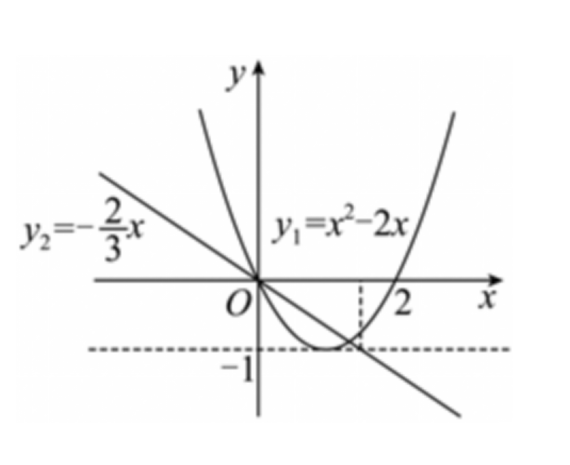
\includegraphics[width=0.24\textwidth]{figures/gao102_q7.png}
\end{center}
\step{当 $m>\dfrac32$ 时，当 $x>m$ 时 $f(x)\in\left(-\infty,-\dfrac23m\right)$，当 $x\leqslant m$ 时 $f(x)\in[-1,+\infty)$，}
\step{显然 $-\dfrac23m<-1$，此时函数 $f(x)$ 的值域不为 $R$，不符合题意；}
\step{当 $m<0$ 时，当 $x>m$ 时，$f(x)\in\left(-\infty,-\dfrac23m\right)$，}
\step{当 $x\leqslant m$ 时，$f(x)\in[m^2-2m,+\infty)$，}
\step{此时 $m^2-2m-\left(-\dfrac23m\right)=m^2-\dfrac43m=m\left(m-\dfrac43\right)>0$，即 $m^2-2m>-\dfrac23m$，}
\step{此时函数 $f(x)$ 的值域不为 $R$，不符合题意；}
\step{当 $0\leqslant m\leqslant\dfrac43$ 时，在 $x\in(0,m)$ 时 $y_2>y_1$，即 $m^2-2m<-\dfrac23m$，}
\step{此时 $f(x)$ 的值域为 $R$，符合题意，}
\step{当 $\dfrac43<m\leqslant\dfrac32$ 时，当 $x>m$ 时，$f(x)\in\left(-\infty,-\dfrac23m\right)$，}
\step{当 $x\leqslant m$ 时，$f(x)\in[-1,+\infty)$，}
\step{此时 $-1-\left(-\dfrac23m\right)=\dfrac23m-1\leqslant0$，即 $-1\leqslant-\dfrac23m$，}
\step{此时函数 $f(x)$ 的值域为 $R$，符合题意；}
\step{综上，$0\leqslant m\leqslant\dfrac32$，即实数 $m$ 的取值范围是 $\left[0,\dfrac32\right]$.}
\solend

\fi

\item 已知函数 $f(x)=x^2-2ax+b$（$a>1$）的定义域和值域都为 $[1,a]$，则 $b=$\blankline[4.4em].

\ifanswer
\solbegin
\step{$f(x)=x^2-2ax+b$（$a>1$）在 $[1,a]$ 严格减，}
\step{则 $f(1)=1-2a+b=a,f(a)=-a^2+b=1$，解得 $a=2,b=5$，所以 $b=5$.}
\solend

\fi

\item 若 $f(x)$ 满足 $f(x+y)=f(x)f(y)$，当 $x>0$ 时，$f(x)$ 的值域为 $(1,+\infty)$，则 $x<0$ 时，
$f(x)$ 的取值范围为\blankline[4.4em].

\ifanswer
\solbegin
\step{因为 $f(x+y)=f(x)f(y)$，令 $x=1$，$y=0$，得 $f(1+0)=f(1)f(0)$，}
\step{又因为当 $x>0$ 时，$f(x)>1$，所以 $f(1)>1>0$，故 $f(0)=1$.}
\step{当 $x<0$ 时，$-x>0$，令 $y=-x$，得 $f(x-x)=f(0)=1=f(x)f(-x)$，}
\step{故 $f(x)=\dfrac1{f(-x)}\in(0,1)$，故 $x<0$ 时，$f(x)$ 的取值范围为 $(0,1)$.}
\solend

\fi

\item 设函数 $f(x)=\begin{cases}x^2+x, & x<0\\ -x^2, & x\geqslant0\end{cases}$，若 $f(f(a))\leqslant2$，则实数 $a$ 的取值范围是\blankline[4.4em].

\ifanswer
\solbegin
\step{函数 $f(x)=\begin{cases}x^2+x, & x<0\\ -x^2, & x\geqslant0\end{cases}$，它的图象如图所示：}
\begin{center}
% 原图第 4 页解析插图直接裁取（原卷排于解析行右侧）。
% 裁框取图形区域，已去粉色水印转灰度。
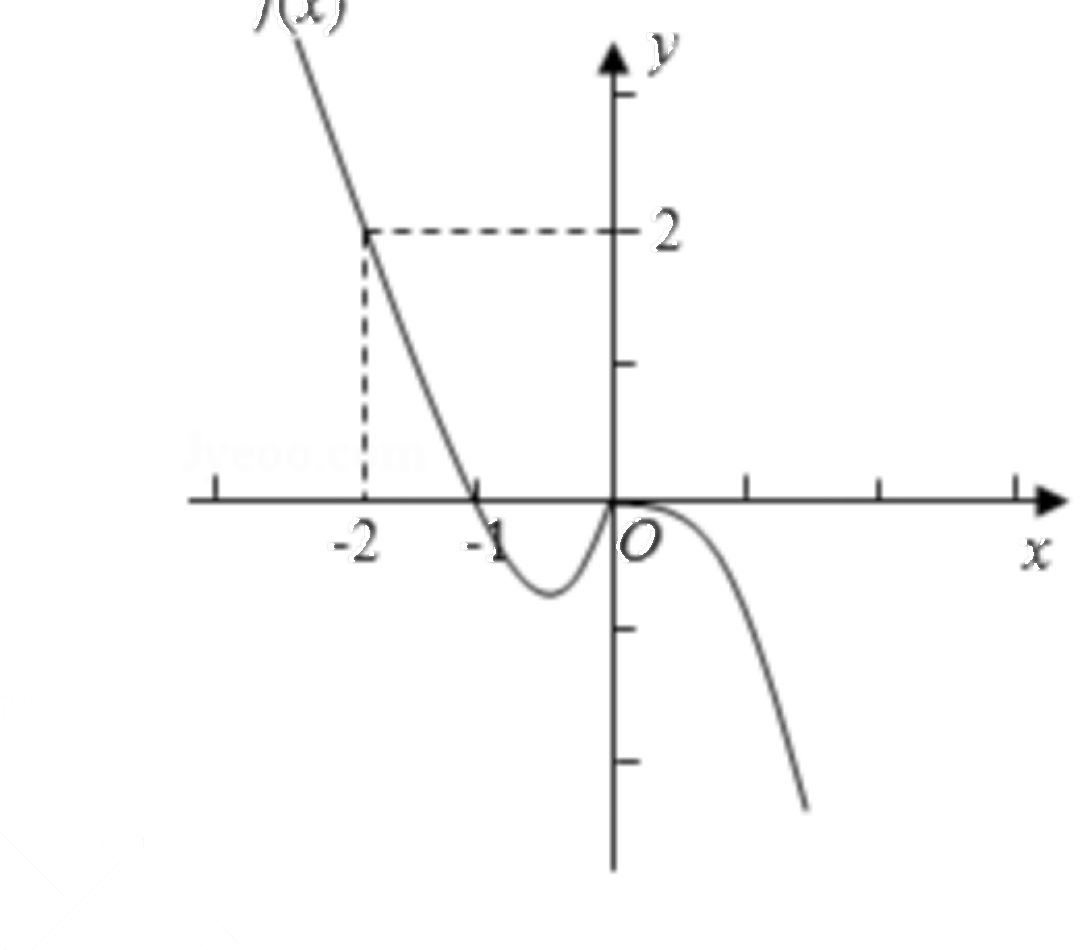
\includegraphics[width=0.30\textwidth]{figures/gao102_q10.png}
\end{center}
\step{由 $f(f(a))\leqslant2$，得 $f(a)\geqslant-2$.}
\step{当 $a<0$ 时，$f(a)=a^2+a=\left(a+\dfrac12\right)^2-\dfrac14\geqslant-2$ 恒成立；}
\step{当 $a\geqslant0$ 时，$f(a)=-a^2\geqslant-2$，即 $a^2\leqslant2$，解得 $0\leqslant a\leqslant\sqrt2$，}
\step{则实数 $a$ 的取值范围是 $(-\infty,\sqrt2]$.}
\solend

\fi

\item 已知二次函数 $f(x)$、$g(x)$ 的二次项系数均为 1，且满足
$\dfrac{f(2025)}{g(2025)}=\dfrac{f(2026)}{g(2026)}=\dfrac{2026}{2025}$，
则 $2026g(2027)-2025f(2027)$ 的值为\blankline[4.4em].

\ifanswer
\solbegin
\step{令 $h(x)=2026g(x)-2025f(x)$，其二次项系数为 $2026-2025=1$.}
\step{由比例条件得 $h(2025)=h(2026)=0$，}
\step{因此 $h(x)=(x-2025)(x-2026),h(2027)=2\times1=2$.}
\solend

\fi

\item 已知函数 $f(x)=\left\lvert x+\dfrac1x-a\right\rvert+1$，对任意实数 $x_1$、$x_2$、$x_3\in\left[\dfrac13,3\right]$，使得以
$f(x_1)$、$f(x_2)$、$f(x_3)$ 数值为边长可构成三角形，则实数 $a$ 的取值范围为\blankline[4.4em].

\ifanswer
\solbegin
\step{对任意实数 $x_1,x_2,x_3\in\left[\dfrac13,3\right]$，}
\step{使得以 $f(x_1)$、$f(x_2)$、$f(x_3)$ 数值为边长可构成三角形，}
\step{只需 $2f(x)_{\min}>f(x)_{\max}$，设 $g(x)=x+\dfrac1x-a$，}
\step{当 $x\in\left[\dfrac13,1\right)$ 时，函数 $g(x)$ 严格减，当 $x\in(1,3]$ 时，函数 $g(x)$ 严格增，}
\step{因为 $g(1)=2-a,g(3)=\dfrac{10}3-a,g\left(\dfrac13\right)=\dfrac{10}3-a$，所以 $g(x)\in\left[2-a,\dfrac{10}3-a\right]$，}
\step{当 $2-a\geqslant0$ 时，即 $a\leqslant2$ 时，$f(x)=\left\lvert x+\dfrac1x-a\right\rvert+1=g(x)+1$，}
\step{此时 $f(x)\in\left[3-a,\dfrac{13}3-a\right]$，}
\step{因此由 $2f(x)_{\min}>f(x)_{\max}\Rightarrow2(3-a)>\dfrac{13}3-a\Rightarrow a<\dfrac53$，而 $a\leqslant2$，所以 $a<\dfrac53$；}
\step{当 $\dfrac{10}3-a\leqslant0$，即 $a\geqslant\dfrac{10}3$ 时，$f(x)=\left\lvert x+\dfrac1x-a\right\rvert+1=-g(x)+1$，}
\step{此时 $f(x)\in\left[a-\dfrac73,a-1\right]$，}
\step{因此由 $2f(x)_{\min}>f(x)_{\max}\Rightarrow2\left(a-\dfrac73\right)>a-1\Rightarrow a>\dfrac{11}3$，而 $a\geqslant\dfrac{10}3$，所以 $a>\dfrac{11}3$，}
\step{若 $2-a<0<\dfrac{10}3-a$ 时，即 $2<a<\dfrac{10}3$ 时，}
\step{若 $a-2\geqslant\dfrac{10}3-a\Rightarrow a\geqslant\dfrac83$，即当 $\dfrac83\leqslant a<\dfrac{10}3$ 时，}
\step{显然此时 $f(x)_{\min}=1$，$f(x)_{\max}=a-2+1=a-1$，}
\step{由 $2f(x)_{\min}>f(x)_{\max}\Rightarrow2\times1>a-1\Rightarrow a<3$，显然 $\dfrac83\leqslant a<3$，}
\step{若 $a-2<\dfrac{10}3-a\Rightarrow a<\dfrac83$，即当 $2<a<\dfrac83$ 时，}
\step{显然此时 $f(x)_{\min}=1,f(x)_{\max}=\dfrac{10}3-a+1=\dfrac{13}3-a$，}
\step{因此由 $2f(x)_{\min}>f(x)_{\max}\Rightarrow2\times1>\dfrac{13}3-a\Rightarrow a>\dfrac73$，而 $\dfrac73<a<\dfrac83$，}
\step{综上，实数 $a$ 的取值范围为 $\left(-\infty,\dfrac53\right)\cup\left(\dfrac73,3\right)\cup\left(\dfrac{11}3,+\infty\right)$.}
\solend

\fi

\end{enumerate}

\bigsec{二、选择题}

\begin{enumerate}
\setcounter{enumi}{12}

\item 已知 $f(x)$ 是定义在 $\R$ 上的奇函数，$g(x)$ 是定义在 $\R$ 上的偶函数，则\mbox{（\quad）}

\keepwithprev
A. $f(x)g(x)$ 是偶函数\qquad B. $f(g(x))$ 是奇函数

C. $f(x)-g(x)$ 是奇函数\qquad D. $g(f(x))$ 是偶函数

\ifanswer
\solbegin
\step{$g(f(x))$ 的定义域为 $\R$，且 $g(f(-x))=g(-f(x))=g(f(x))$，}
\step{所以 $g(f(x))$ 是偶函数，故选 $D$.}
\solend

\fi

\item 已知定义在 $R$ 上的偶函数 $f(x)=\lvert x-m+1\rvert-2$，若正实数 $a$、$b$ 满足 $f(a)+f(2b)=m$，
则 $\dfrac1a+\dfrac2b$ 的最小值为\mbox{（\quad）}

\keepwithprev
A. $\dfrac95$\qquad\qquad B. $9$\qquad\qquad C. $\dfrac85$\qquad\qquad D. $8$

\ifanswer
\solbegin
\step{因为 $f(x)=\lvert x-m+1\rvert-2$ 是偶函数，所以 $-m+1=0$，所以 $m=1$，}
\step{所以 $f(x)=\lvert x\rvert-2$，若正实数 $a$、$b$ 满足 $f(a)+f(2b)=m$，}
\step{则 $a-2+2b-2=1$，所以 $a+2b=5$，}
\step{所以 $\dfrac1a+\dfrac2b=\dfrac15(a+2b)\left(\dfrac1a+\dfrac2b\right)=\dfrac15\left(5+\dfrac{2a}b+\dfrac{2b}a\right)\geqslant\dfrac95$，}
\step{当且仅当 $a=b=\dfrac53$ 时取等号，则 $\dfrac1a+\dfrac2b$ 的最小值为 $\dfrac95$，故选 $A$.}
\solend

\fi

\item 设函数 $g(x)=x^2-2$（$x\in\R$），$f(x)=\begin{cases}g(x)+x+4, & x<g(x)\\ g(x)-x, & x\geqslant g(x)\end{cases}$，则 $f(x)$ 的值域是

\mbox{（\quad）}

\keepwithprev
A. $\left[-\dfrac94,0\right]\cup(1,+\infty)$\qquad\qquad B. $[0,+\infty)$

C. $\left[-\dfrac94,+\infty\right)$\qquad\qquad D. $\left[-\dfrac94,0\right]\cup(2,+\infty)$

\ifanswer
\solbegin
\step{当 $x<g(x)$，即 $x<x^2-2$，$(x-2)(x+1)>0$ 时，$x>2$ 或 $x<-1$，}
\step{$f(x)=g(x)+x+4=x^2-2+x+4=x^2+x+2=(x+0.5)^2+1.75$，}
\step{其最小值趋向于 $f(-1)$ 即 2，无最大值，}
\step{因此这个区间的值域为 $(2,+\infty)$.}
\step{当 $x\geqslant g(x)$ 时，$-1\leqslant x\leqslant2$，$f(x)=g(x)-x=x^2-2-x=(x-0.5)^2-2.25$，}
\step{其最小值为 $f(0.5)=-2.25$，其最大值为 $f(2)=0$，}
\step{因此这区间的值域为 $[-2.25,0]$.}
\step{综上，函数值域为 $\left[-\dfrac94,0\right]\cup(2,+\infty)$，故选 $D$.}
\solend

\fi

\item 设 $D$ 是含数 1 的有限实数集，$f(x)$ 是定义在 $D$ 上的函数，若 $f(x)$ 的图象绕原点逆时针
旋转 $\dfrac{\pi}{6}$ 与原图象重合，则在以下各项中，$f(1)$ 的可能取值只能是\mbox{（\quad）}

\keepwithprev
A. $\sqrt3$\qquad\qquad B. $\dfrac{\sqrt3}2$\qquad\qquad C. $\dfrac{\sqrt3}3$\qquad\qquad D. $0$

\ifanswer
\solbegin
\step{问题相当于圆上由 12 个点为一组，每次绕原点逆时针旋转 $\dfrac{\pi}{6}$ 个单位后与下一个点}
\step{会重合。我们可以通过代入和赋值的方法，当 $f(1)=\sqrt3$、$\dfrac{\sqrt3}3$、$0$ 时，}
\step{此时得到的圆心角为 $\dfrac{\pi}{3}$、$\dfrac{\pi}{6}$、$0$，然而此时 $x=0$ 或者 $x=1$ 时，}
\step{都有 2 个 $y$ 与之对应，而我们知道函数的定义就是要求一个 $x$ 只能对应一个 $y$，}
\step{因此只有当 $x=\dfrac{\sqrt3}2$，此时旋转 $\dfrac{\pi}{6}$，此时满足一个 $x$ 只会对应一个 $y$，故选 $B$.}
\solend

\fi

\end{enumerate}

\bigsec{三、解答题}

\begin{enumerate}
\setcounter{enumi}{16}

\item 求下列函数的值域.

（1）$y=\dfrac{2x^2-3x+5}{x-1}\left(x\in\left[\dfrac32,3\right]\right)$；

（2）$f(x)=\sqrt{x}-\sqrt{2-x}+\sqrt{x(2-x)}$.

\ansspace*[10]

\ifanswer
\solbegin
\stepm{（1）}{令 $t=x-1$，则 $t\in\left[\dfrac12,2\right]$，原函数化为 $Y(t)=2t+\dfrac4t+1$.}
\step{当 $0<u<v$ 时，$Y(v)-Y(u)=2(v-u)\left(1-\dfrac2{uv}\right)$，}
\step{所以 $Y$ 在 $\left[\dfrac12,\sqrt2\right]$ 上严格递减，在 $[\sqrt2,2]$ 上严格递增.}
\step{由 $Y(\sqrt2)=4\sqrt2+1,Y\left(\dfrac12\right)=10,Y(2)=7$，得值域为 $[4\sqrt2+1,10]$.}
\stepm{（2）}{定义域为 $[0,2]$.}
\step{令 $s=\sqrt{x}-\sqrt{2-x}$，$\sqrt{x}$ 与 $-\sqrt{2-x}$ 均随 $x$ 严格递增，}
\step{$s$ 从 $-\sqrt2$ 递增到 $\sqrt2$，即 $s\in[-\sqrt2,\sqrt2]$.}
\step{由 $s^2=2-2\sqrt{x(2-x)}$，得 $f(x)=s+\dfrac{2-s^2}2=-\dfrac12(s-1)^2+\dfrac32$.}
\step{当 $s=1$ 时取得最大值 $\dfrac32$；当 $s=-\sqrt2$ 时取得最小值 $-\sqrt2$；}
\step{因此值域为 $\left[-\sqrt2,\dfrac32\right]$.}
\solend

\fi

\item 已知 $f(2x+1)=\dfrac{2x+1}{x+1}$.

（1）解不等式 $f(x)<x$；

（2）求 $f(1)+f(2)+\cdots+f(6)+f\left(\dfrac12\right)+f\left(\dfrac13\right)+\cdots+f\left(\dfrac16\right)$ 的值.

\ansspace*[12]

\ifanswer
\solbegin
\step{令 $t=2x+1$，则 $x=\dfrac{t-1}2$，得 $f(t)=\dfrac{2t}{t+1},t\neq-1$.}
\stepm{（1）}{不等式等价于 $\dfrac{2x}{x+1}<x\Leftrightarrow\dfrac{x(x-1)}{x+1}>0$.}
\step{以 $-1,0,1$ 分区间判断符号，得解集为 $(-1,0)\cup(1,+\infty)$.}
\stepm{（2）}{当 $x>0$ 时，$f(x)+f\left(\dfrac1x\right)=\dfrac{2x}{x+1}+\dfrac2{x+1}=2$.}
\step{将 $f(2),\cdots,f(6)$ 分别与其倒数对应的函数值配对，共 5 对，且 $f(1)=1$，}
\step{因此原式$=1+5\times2=11$.}
\solend

\fi

\item 已知函数 $f(x)$、$g(x)$ 是定义在 $R$ 上的函数，其中 $f(x)$ 是奇函数，$g(x)$ 是偶函数，且
$f(x)+g(x)=ax^2-x$.

（1）求 $f(x)$ 和 $g(x)$ 的解析式；

（2）$h(x)=f(x)+g(x)+(1-a)x^2-2ax+4$ 在 $[1,3]$ 上有两个零点，求实数 $a$ 的取值范
围.

\ansspace*[14]

\ifanswer
\solbegin
\stepm{（1）}{因为 $f(x)+g(x)=ax^2-x$①，所以 $f(-x)+g(-x)=ax^2+x$，}
\step{又 $f(x)$ 是奇函数，$g(x)$ 是偶函数，}
\step{所以 $f(-x)=-f(x)$，$g(-x)=g(x)$，}
\step{所以 $-f(x)+g(x)=ax^2+x$②，}
\step{联立①②解得 $f(x)=-x$，$g(x)=ax^2$.}
\stepm{（2）}{$h(x)=f(x)+g(x)+(1-a)x^2-2ax+4$}
\step{$=ax^2-x+(1-a)x^2-2ax+4=x^2-(2a+1)x+4$，}
\step{是开口向上，对称轴为 $x=\dfrac{2a+1}2$ 的二次函数，}
\step{因为 $h(x)$ 在 $[1,3]$ 上有两个零点，所以 $\begin{cases}\Delta=(2a+1)^2-16>0\\ 1<\dfrac{2a+1}2<3\\ h(1)=1-(2a+1)+4\geqslant0\\ h(3)=9-3(2a+1)+4\geqslant0\end{cases}$，}
\step{解得 $\dfrac32<a\leqslant\dfrac53$，故实数 $a$ 的取值范围为 $\left(\dfrac32,\dfrac53\right]$.}
\solend

\fi

\item 若函数 $f(x)$ 在区间 $[a,b]$ 上的值域恰为 $\left[\dfrac1b,\dfrac1a\right]$，则称区间 $[a,b]$ 为 $f(x)$ 的一个“倒域
区间”。已知定义在 $[-4,4]$ 上的奇函数 $g(x)$，当 $x\in[0,4]$ 时，$g(x)=-x^2+2x$.

（1）求 $g(x)$ 的解析式；

（2）若关于 $x$ 的方程 $g(x)=-mx-m$ 在 $(0,4)$ 上恰有两个不相等的实数根，求实数 $m$ 的
取值范围；

（3）求函数 $g(x)$ 在 $[-4,0]$ 内的“倒域区间”.

\ansspace*[16]

\ifanswer
\solbegin
\stepm{（1）}{当 $x\in[-4,0)$ 时，$-x\in(0,4]$，}
\step{由奇函数的定义得 $g(x)=-g(-x)=-[(-x)^2+2(-x)]=x^2+2x$，}
\step{所以 $g(x)=\begin{cases}-x^2+2x, & 0\leqslant x\leqslant4\\ x^2+2x, & -4\leqslant x<0\end{cases}$.}
\stepm{（2）}{方程 $g(x)=-mx-m$，即 $x^2-(m+2)x-m=0$，}
\step{设 $h(x)=x^2-(m+2)x-m$，$0<x<4$，}
\step{由题意得 $\begin{cases}h(0)=-m>0\\ h(4)=8-5m>0\\ \Delta=(m+2)^2+4m>0\\ 0<\dfrac{m+2}2<4\end{cases}$，解得 $2\sqrt3-4<m<0$，}
\step{即实数 $m$ 的取值范围是 $(2\sqrt3-4,0)$.}
\stepm{（3）}{易得当 $-4\leqslant a<b<0$ 时，$\dfrac1b<\dfrac1a$，}
\step{且 $g(x)$ 在 $[-4,-1]$ 上严格减，在 $[-1,0]$ 上严格增，}
\step{故当 $x\in[-4,0]$ 时，$g(x)_{\min}=g(-1)=-1$，}
\step{所以 $\dfrac1b\geqslant-1$，所以 $-4<b\leqslant-1$，所以 $-4\leqslant a<b\leqslant-1$，}
\step{则 $\begin{cases}g(a)=a^2+2a=\dfrac1a\\ g(b)=b^2+2b=\dfrac1b\\ -4\leqslant a<b\leqslant-1\end{cases}$，解得 $\begin{cases}a=-\dfrac{1+\sqrt5}2\\ b=-1\end{cases}$，}
\step{所以 $g(x)$ 在 $[-4,0]$ 内的“倒域区间”为 $\left[-\dfrac{1+\sqrt5}2,-1\right]$.}
\solend

\fi

\item 我们知道：函数 $y=f(x)$ 的图象关于坐标原点成中心对称图形的充要条件是函数
$y=f(x)$ 为奇函数。有同学发现可以推广为：函数 $y=f(x)$ 的图象关于点 $(a,b)$ 成中心对
称图形的充要条件为函数 $y=f(x+a)-b$ 为奇函数。已知函数 $f(x)=\dfrac{2x}{3-x}$.

（1）求函数 $f(x)$ 图象的对称中心；

（2）若定义在 $R$ 上的函数 $y=g(x)$ 的图象关于点 $(1,2)$ 对称，且 $g(1)=2$，当 $x\in[0,1)$
时，$g(x)=x^2-tx+t+1$.

（$i$）求 $g(-3)+g(5)$ 的值；

（$ii$）若对$\forall x_1\in[0,2]$，$\exists x_2\in[-3,2]$ 使得 $g(x_1)=f(x_2)$ 恒成立，求实数 $t$ 的取值范围.

\ansspace*[18]

\ifanswer
\solbegin
\stepm{（1）}{由 $f(x)=\dfrac{2x}{3-x}=-2+\dfrac6{3-x}$，}
\step{易得 $f(x+3)+2=-2+\dfrac6{3-(x+3)}+2=-\dfrac6x$ 为奇函数，}
\step{$f(x)$ 的图象关于 $(3,-2)$ 对称.}
\stepm{（2）}{（$i$）$y=g(x)$ 图象关于点 $(1,2)$ 对称，则 $g(1+x)+g(1-x)=4$，}
\step{令 $x=4$，则 $g(-3)+g(5)=4$.}
\step{（$ii$）有 $g(x)$ 在 $x\in[0,2]$ 的取值范围为 $f(x)$ 在 $x\in[-3,2]$ 的取值范围的}
\step{子集，}
\step{因为 $f(x)=\dfrac{2x}{3-x}=\dfrac{6-2(3-x)}{3-x}=\dfrac6{3-x}-2$ 在 $[-3,2]$ 上严格增，}
\step{所以 $f(x)$ 在 $x\in[-3,2]$ 上的取值范围为 $[-1,4]$，}
\step{记 $g(x)$ 的值域为 $A$，且 $g(1)=2$，当 $x\in[0,1)$ 时 $g(x)=x^2-tx+t+1$，}
\step{①当 $\dfrac t2\leqslant0$，即 $t\leqslant0$ 时，有 $g(x)$ 在 $[0,1)$ 上严格增，}
\step{由对称性得 $g(x)$ 在 $[1,2]$ 上严格增，故 $g(x)$ 在 $[0,2]$ 上严格增，}
\step{故 $g(x)_{\min}=g(0)=t+1$，$g(x)_{\max}=g(2)=4-(t+1)=3-t$，$t\leqslant0$，}
\step{则 $A=[t+1,3-t]\subseteq[-1,4]$，即 $\begin{cases}t\leqslant0\\ t+1\geqslant-1\\ 3-t\leqslant4\end{cases}$，解得 $-1\leqslant t\leqslant0$.}
\step{②当 $0<\dfrac t2<1$，即 $0<t<2$ 时，}
\step{$g(x)$ 在 $\left(0,\dfrac t2\right)$ 上严格减，在 $\left(\dfrac t2,1\right)$ 上严格增，}
\step{由对称性得 $g(x)$ 在 $\left(2-\dfrac t2,2\right)$ 上严格减，在 $\left(1,2-\dfrac t2\right)$ 上严格增，}
\step{故 $g(x)$ 在 $\left(0,\dfrac t2\right)$ 上严格减，在 $\left(\dfrac t2,2-\dfrac t2\right)$ 上严格增，}
\step{在 $\left(2-\dfrac t2,2\right)$ 上严格减，则 $A=\left[g\left(\dfrac t2\right),g\left(2-\dfrac t2\right)\right]$，}
\step{由 $0<t<2$，得 $g(0)=t+1\in(1,3)$，$g(2)=4-(t+1)=3-t\in(1,3)$，}
\step{$g\left(\dfrac t2\right)=-\dfrac{t^2}4+t+1=-\dfrac14(t-2)^2+2\in(1,2]$，}
\step{又 $g\left(\dfrac t2\right)+g\left(2-\dfrac t2\right)=4$，$g\left(2-\dfrac t2\right)\in(2,3)$，}
\step{当 $0<t<2$ 时，$A\subseteq[-1,4]$ 恒成立，}
\step{③当 $\dfrac t2\geqslant1$，即 $t\geqslant2$ 时，有 $g(x)$ 在 $[0,1)$ 上严格减，}
\step{由对称点 $(1,2)$ 得 $g(x)$ 在 $[1,2]$ 上严格减，所以 $g(x)$ 在 $[0,2]$ 上严格减，}
\step{故 $g(x)_{\max}=g(0)=t+1$，$g(x)_{\min}=g(2)=4-(t+1)=3-t$，$t\geqslant2$，}
\step{则 $A=[3-t,t+1]\subseteq[-1,4]$，即 $\begin{cases}t\geqslant2\\ t+1\leqslant4\\ 3-t\geqslant-1\end{cases}$，解得 $2\leqslant t\leqslant3$.}
\step{综上，$t$ 的范围为 $\{t\mid-1\leqslant t\leqslant3\}$.}
\solend

\fi

\end{enumerate}

\end{document}
"
%
% 原始材料：微信公众号“魔都数学加油站”文章，作者破晓，2026-11-01 21:56 发布；
% 连载“27学年高一102”，原文标题“27学年高一102——2026-2027年上海市华师大二附中高一上周末作业5函数”；
% 原文链接：https://mp.weixin.qq.com/s/CDvOCcxFskIe9aFUeKi3Ww。
% 正文为 13 张 PNG 页（第 1、2、10、13 页 2560×3620，其余 4762×6735），题目下印有【解析】，为讲评版。
% 题目、解析均据原图转录；卷面水印及公众号页脚未录入。
%
% 卷首标题：原卷印作“2026-2027 年华师大二附中高一上周末作业 5”（公众号标题中的“上海市”“函数”
% 卷面标题行没有，本稿照卷面），年份区间按全稿惯例排 en dash；原卷未印副标题，本稿按题目内容
% 标为“函数”（全稿首份以函数为单一模块的卷子）。
%
% 与原卷的排版差异：
%   ① 原文从第 3 题起，填空题编号为 3—12、选择题为 13—16、解答题为 17—21，本稿保留原题号；
%   ② 原卷每题下直接印【解析】，本稿按全稿惯例将解析置于答案版；选择题括号内未印答案，另由
%      解析末句“故选 X”给出；
%   ③ 原卷未印副标题，本稿按“知识模块”口径补出；
%   ④ 原卷填空横线按全稿惯例排为 \blankline[4.4em]；解答题按惯例加 \ansspace；选择题括号排
%      \mbox{（\quad）}、选项段前按惯例加 \keepwithprev；
%   ⑤ 原卷 $f(x)_{min}$、$f(x)_{max}$ 等下标排斜体，按 高一96 成例改正体 $\min$、$\max$；
%   ⑥ 原卷数集排斜体 $R$（第 13 题排粗体），按全稿惯例改 $\R$；
%   ⑦ 第 7、10 两题的解析插图裁自原图（去粉色水印转灰度），仅答案版显示。
%
% 原卷存疑／笔误（均照录加注）：
%   第 3 题解析“减去都对应 −2 和 2 的”措辞含糊（意为减去恒取 −2 与恒取 2 的两个常函数）；
%   第 15 题解析“其最小值趋向于 f(−1) 即 2”（该段 f(x)=x²+x+2 在 x→−1⁻ 时趋于 2、取不到）；
%   第 16 题解析末句“因此只有当 x=√3/2”（按上下文应为 f(1)=√3/2）；
%   第 16 题解析以 f(1)=√3、√3/3、0 赋值时称“得到的圆心角为 π/3、π/6、0”，其中 √3/3 对应
%   圆心角 π/6 的说法与该点 (1,√3/3) 的实际幅角一致，但与选项 C（√3/3）被排除的结论矛盾
%   （幅角 π/6 的点旋转 π/6 后落到幅角 π/3 处，仍占 12 等分点位，原卷解析未展开），照录。
%
% 行数核对：逐题数 \step/\stepm 条数，合计 155 条（Q3：2；Q4：3；Q5：6；Q6：5；Q7：19；
% Q8：2；Q9：4；Q10：5；Q11：3；Q12：19；Q13：2；Q14：5；Q15：8；Q16：5；Q17：10；
% Q18：6；Q19：10；Q20：13；Q21：28），与原卷印刷行逐题相等。
%
\documentclass[a4paper,11pt]{article}
\usepackage{common}

\begin{document}

\examtitlest[3]{2026--2027 年华师大二附中高一上周末作业 5}{函数}

\bigsec{一、填空题}

\begin{enumerate}
\setcounter{enumi}{2}

\item 已知函数 $y=f(x)$ 的定义域为 $\{-2,-1,1,2\}$，值域为 $\{-2,2\}$，则满足条件的函数
$y=f(x)$ 最多有\blankline[4.4em]个.

\ifanswer
\solbegin
\step{定义域中 4 个元素每个都可以对应 $-2$ 和 $2$ 中的一个，减去都对应 $-2$ 和 $2$ 的，}
\step{则满足条件的函数 $y=f(x)$ 最多有 $2^4-2=14$.}
\solend

\fi

\item 已知函数 $f(2x)$ 的定义域为 $[-2,2]$，则函数 $f(x-3)$ 的定义域为\blankline[4.4em].

\ifanswer
\solbegin
\step{因为函数 $f(2x)$ 的定义域为 $[-2,2]$，即 $-2\leqslant x\leqslant2$，所以 $-4\leqslant2x\leqslant4$，}
\step{得 $f(x)$ 的定义域为 $[-4,4]$，由 $-4\leqslant x-3\leqslant4$，解得 $-1\leqslant x\leqslant7$，}
\step{即函数 $f(x-3)$ 的定义域为 $[-1,7]$.}
\solend

\fi

\item 函数 $f(x)=\begin{cases}-x-1, & x<0\\ -x+1, & x>0\end{cases}$，则 $f(x)-f(-x)>1$ 的解集为\blankline[4.4em].

\ifanswer
\solbegin
\step{定义域为 $\{x\mid x\neq0\}$.}
\step{当 $x<0$ 时，$-x>0,f(-x)=x+1$，}
\step{$f(x)-f(-x)=(-x-1)-(x+1)=-2x-2>1$，得 $x<-\dfrac32$.}
\step{当 $x>0$ 时，$f(-x)=x-1,f(x)-f(-x)=(-x+1)-(x-1)=-2x+2>1$，}
\step{得 $0<x<\dfrac12$.}
\step{故解集为 $\left(-\infty,-\dfrac32\right)\cup\left(0,\dfrac12\right)$.}
\solend

\fi

\item 已知函数 $f(x)=x^2-2(m-3)x+5$ 在区间 $[2,+\infty)$ 上的最小值为 1，则实数 $m=$\blankline[4.4em].

\ifanswer
\solbegin
\step{函数 $f(x)$ 图象的对称轴为 $x=m-3$.}
\step{当 $m-3\leqslant2$，即 $m\leqslant5$ 时，$f(x)_{\min}=f(2)=9-4m+12=1$，解得 $m=5$；}
\step{当 $m-3>2$，即 $m>5$ 时，$f(x)_{\min}=f(m-3)=-m^2+6m-4=1$，}
\step{解得 $m=5$（舍去）或 $1$（舍去），}
\step{综上，$m=5$.}
\solend

\fi

\item 已知函数 $f(x)=\begin{cases}x^2-2x, & x\leqslant m\\ -\dfrac23x, & x>m\end{cases}$ 的值域为 $R$，则实数 $m$ 的取值范围是\blankline[4.4em].

\ifanswer
\solbegin
\step{对于函数 $y_1=x^2-2x$，则 $y_1=(x-1)^2-1\geqslant-1$，当且仅当 $x=1$ 时取等号，}
\step{且函数在 $(-\infty,1)$ 上严格减，在 $(1,+\infty)$ 上严格增，}
\step{对于函数 $y_2=-\dfrac23x$，令 $y_2=-1$，则 $x=\dfrac32$，且函数在定义域上严格减，}
\step{令 $x^2-2x=-\dfrac23x$，解得 $x=0$ 或 $x=\dfrac43$，}
\step{所以 $y_2=-\dfrac23x$ 与 $y_1=x^2-2x$ 的两个交点分别为 $(0,0)$、$\left(\dfrac43,-\dfrac89\right)$，}
\step{则函数 $y_2=-\dfrac23x$ 与 $y_1=x^2-2x$ 的图象如图所示：}
\begin{center}
% 原图第 2 页解析插图直接裁取（原卷排于解析行右侧）。
% 裁框取图形区域，已去粉色水印转灰度。
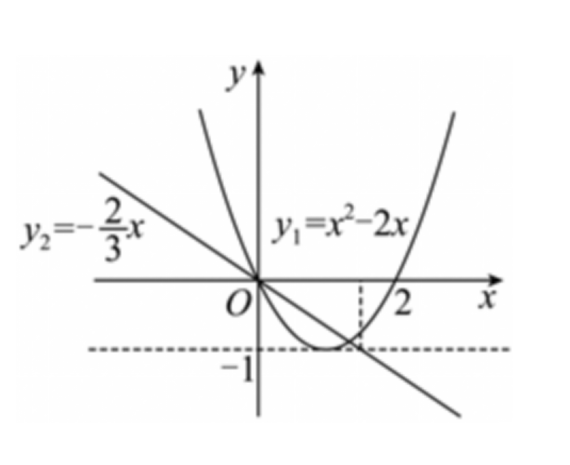
\includegraphics[width=0.24\textwidth]{figures/gao102_q7.png}
\end{center}
\step{当 $m>\dfrac32$ 时，当 $x>m$ 时 $f(x)\in\left(-\infty,-\dfrac23m\right)$，当 $x\leqslant m$ 时 $f(x)\in[-1,+\infty)$，}
\step{显然 $-\dfrac23m<-1$，此时函数 $f(x)$ 的值域不为 $R$，不符合题意；}
\step{当 $m<0$ 时，当 $x>m$ 时，$f(x)\in\left(-\infty,-\dfrac23m\right)$，}
\step{当 $x\leqslant m$ 时，$f(x)\in[m^2-2m,+\infty)$，}
\step{此时 $m^2-2m-\left(-\dfrac23m\right)=m^2-\dfrac43m=m\left(m-\dfrac43\right)>0$，即 $m^2-2m>-\dfrac23m$，}
\step{此时函数 $f(x)$ 的值域不为 $R$，不符合题意；}
\step{当 $0\leqslant m\leqslant\dfrac43$ 时，在 $x\in(0,m)$ 时 $y_2>y_1$，即 $m^2-2m<-\dfrac23m$，}
\step{此时 $f(x)$ 的值域为 $R$，符合题意，}
\step{当 $\dfrac43<m\leqslant\dfrac32$ 时，当 $x>m$ 时，$f(x)\in\left(-\infty,-\dfrac23m\right)$，}
\step{当 $x\leqslant m$ 时，$f(x)\in[-1,+\infty)$，}
\step{此时 $-1-\left(-\dfrac23m\right)=\dfrac23m-1\leqslant0$，即 $-1\leqslant-\dfrac23m$，}
\step{此时函数 $f(x)$ 的值域为 $R$，符合题意；}
\step{综上，$0\leqslant m\leqslant\dfrac32$，即实数 $m$ 的取值范围是 $\left[0,\dfrac32\right]$.}
\solend

\fi

\item 已知函数 $f(x)=x^2-2ax+b$（$a>1$）的定义域和值域都为 $[1,a]$，则 $b=$\blankline[4.4em].

\ifanswer
\solbegin
\step{$f(x)=x^2-2ax+b$（$a>1$）在 $[1,a]$ 严格减，}
\step{则 $f(1)=1-2a+b=a,f(a)=-a^2+b=1$，解得 $a=2,b=5$，所以 $b=5$.}
\solend

\fi

\item 若 $f(x)$ 满足 $f(x+y)=f(x)f(y)$，当 $x>0$ 时，$f(x)$ 的值域为 $(1,+\infty)$，则 $x<0$ 时，
$f(x)$ 的取值范围为\blankline[4.4em].

\ifanswer
\solbegin
\step{因为 $f(x+y)=f(x)f(y)$，令 $x=1$，$y=0$，得 $f(1+0)=f(1)f(0)$，}
\step{又因为当 $x>0$ 时，$f(x)>1$，所以 $f(1)>1>0$，故 $f(0)=1$.}
\step{当 $x<0$ 时，$-x>0$，令 $y=-x$，得 $f(x-x)=f(0)=1=f(x)f(-x)$，}
\step{故 $f(x)=\dfrac1{f(-x)}\in(0,1)$，故 $x<0$ 时，$f(x)$ 的取值范围为 $(0,1)$.}
\solend

\fi

\item 设函数 $f(x)=\begin{cases}x^2+x, & x<0\\ -x^2, & x\geqslant0\end{cases}$，若 $f(f(a))\leqslant2$，则实数 $a$ 的取值范围是\blankline[4.4em].

\ifanswer
\solbegin
\step{函数 $f(x)=\begin{cases}x^2+x, & x<0\\ -x^2, & x\geqslant0\end{cases}$，它的图象如图所示：}
\begin{center}
% 原图第 4 页解析插图直接裁取（原卷排于解析行右侧）。
% 裁框取图形区域，已去粉色水印转灰度。
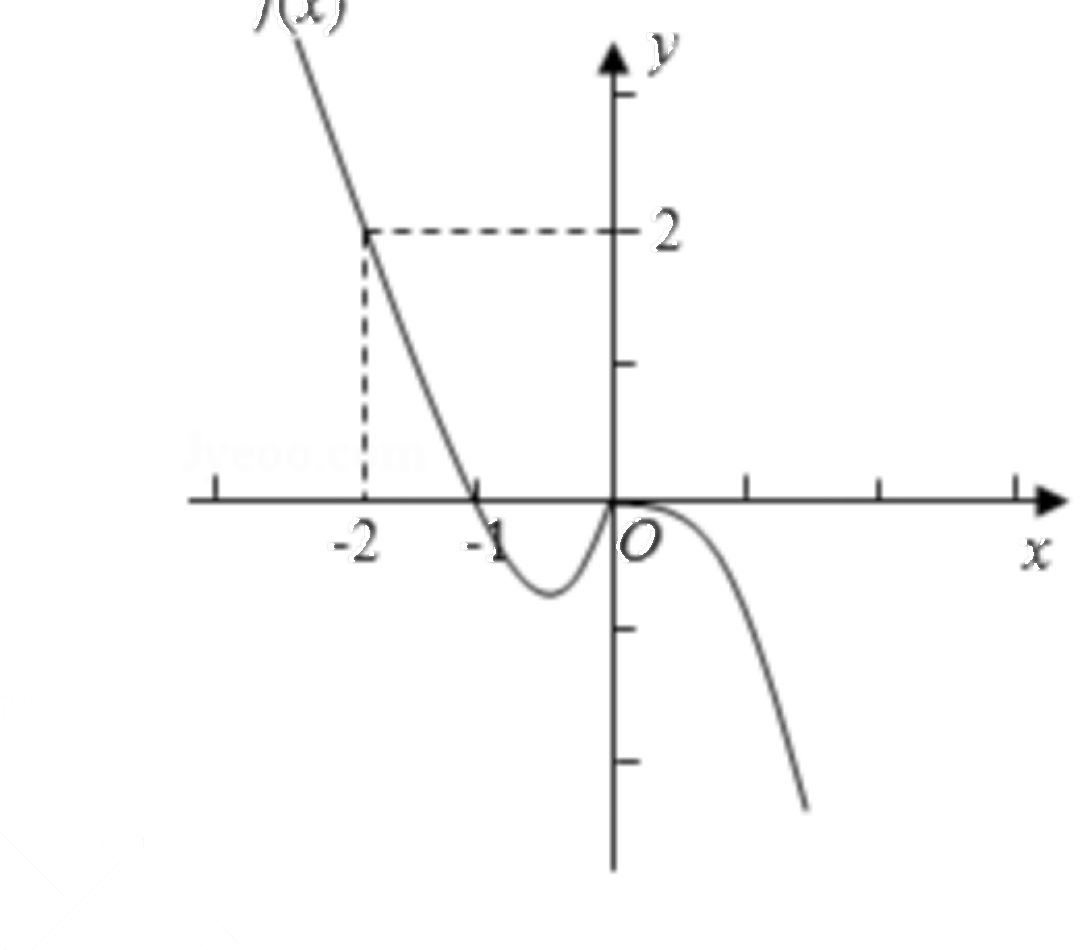
\includegraphics[width=0.30\textwidth]{figures/gao102_q10.png}
\end{center}
\step{由 $f(f(a))\leqslant2$，得 $f(a)\geqslant-2$.}
\step{当 $a<0$ 时，$f(a)=a^2+a=\left(a+\dfrac12\right)^2-\dfrac14\geqslant-2$ 恒成立；}
\step{当 $a\geqslant0$ 时，$f(a)=-a^2\geqslant-2$，即 $a^2\leqslant2$，解得 $0\leqslant a\leqslant\sqrt2$，}
\step{则实数 $a$ 的取值范围是 $(-\infty,\sqrt2]$.}
\solend

\fi

\item 已知二次函数 $f(x)$、$g(x)$ 的二次项系数均为 1，且满足
$\dfrac{f(2025)}{g(2025)}=\dfrac{f(2026)}{g(2026)}=\dfrac{2026}{2025}$，
则 $2026g(2027)-2025f(2027)$ 的值为\blankline[4.4em].

\ifanswer
\solbegin
\step{令 $h(x)=2026g(x)-2025f(x)$，其二次项系数为 $2026-2025=1$.}
\step{由比例条件得 $h(2025)=h(2026)=0$，}
\step{因此 $h(x)=(x-2025)(x-2026),h(2027)=2\times1=2$.}
\solend

\fi

\item 已知函数 $f(x)=\left\lvert x+\dfrac1x-a\right\rvert+1$，对任意实数 $x_1$、$x_2$、$x_3\in\left[\dfrac13,3\right]$，使得以
$f(x_1)$、$f(x_2)$、$f(x_3)$ 数值为边长可构成三角形，则实数 $a$ 的取值范围为\blankline[4.4em].

\ifanswer
\solbegin
\step{对任意实数 $x_1,x_2,x_3\in\left[\dfrac13,3\right]$，}
\step{使得以 $f(x_1)$、$f(x_2)$、$f(x_3)$ 数值为边长可构成三角形，}
\step{只需 $2f(x)_{\min}>f(x)_{\max}$，设 $g(x)=x+\dfrac1x-a$，}
\step{当 $x\in\left[\dfrac13,1\right)$ 时，函数 $g(x)$ 严格减，当 $x\in(1,3]$ 时，函数 $g(x)$ 严格增，}
\step{因为 $g(1)=2-a,g(3)=\dfrac{10}3-a,g\left(\dfrac13\right)=\dfrac{10}3-a$，所以 $g(x)\in\left[2-a,\dfrac{10}3-a\right]$，}
\step{当 $2-a\geqslant0$ 时，即 $a\leqslant2$ 时，$f(x)=\left\lvert x+\dfrac1x-a\right\rvert+1=g(x)+1$，}
\step{此时 $f(x)\in\left[3-a,\dfrac{13}3-a\right]$，}
\step{因此由 $2f(x)_{\min}>f(x)_{\max}\Rightarrow2(3-a)>\dfrac{13}3-a\Rightarrow a<\dfrac53$，而 $a\leqslant2$，所以 $a<\dfrac53$；}
\step{当 $\dfrac{10}3-a\leqslant0$，即 $a\geqslant\dfrac{10}3$ 时，$f(x)=\left\lvert x+\dfrac1x-a\right\rvert+1=-g(x)+1$，}
\step{此时 $f(x)\in\left[a-\dfrac73,a-1\right]$，}
\step{因此由 $2f(x)_{\min}>f(x)_{\max}\Rightarrow2\left(a-\dfrac73\right)>a-1\Rightarrow a>\dfrac{11}3$，而 $a\geqslant\dfrac{10}3$，所以 $a>\dfrac{11}3$，}
\step{若 $2-a<0<\dfrac{10}3-a$ 时，即 $2<a<\dfrac{10}3$ 时，}
\step{若 $a-2\geqslant\dfrac{10}3-a\Rightarrow a\geqslant\dfrac83$，即当 $\dfrac83\leqslant a<\dfrac{10}3$ 时，}
\step{显然此时 $f(x)_{\min}=1$，$f(x)_{\max}=a-2+1=a-1$，}
\step{由 $2f(x)_{\min}>f(x)_{\max}\Rightarrow2\times1>a-1\Rightarrow a<3$，显然 $\dfrac83\leqslant a<3$，}
\step{若 $a-2<\dfrac{10}3-a\Rightarrow a<\dfrac83$，即当 $2<a<\dfrac83$ 时，}
\step{显然此时 $f(x)_{\min}=1,f(x)_{\max}=\dfrac{10}3-a+1=\dfrac{13}3-a$，}
\step{因此由 $2f(x)_{\min}>f(x)_{\max}\Rightarrow2\times1>\dfrac{13}3-a\Rightarrow a>\dfrac73$，而 $\dfrac73<a<\dfrac83$，}
\step{综上，实数 $a$ 的取值范围为 $\left(-\infty,\dfrac53\right)\cup\left(\dfrac73,3\right)\cup\left(\dfrac{11}3,+\infty\right)$.}
\solend

\fi

\end{enumerate}

\bigsec{二、选择题}

\begin{enumerate}
\setcounter{enumi}{12}

\item 已知 $f(x)$ 是定义在 $\R$ 上的奇函数，$g(x)$ 是定义在 $\R$ 上的偶函数，则\mbox{（\quad）}

\keepwithprev
A. $f(x)g(x)$ 是偶函数\qquad B. $f(g(x))$ 是奇函数

C. $f(x)-g(x)$ 是奇函数\qquad D. $g(f(x))$ 是偶函数

\ifanswer
\solbegin
\step{$g(f(x))$ 的定义域为 $\R$，且 $g(f(-x))=g(-f(x))=g(f(x))$，}
\step{所以 $g(f(x))$ 是偶函数，故选 $D$.}
\solend

\fi

\item 已知定义在 $R$ 上的偶函数 $f(x)=\lvert x-m+1\rvert-2$，若正实数 $a$、$b$ 满足 $f(a)+f(2b)=m$，
则 $\dfrac1a+\dfrac2b$ 的最小值为\mbox{（\quad）}

\keepwithprev
A. $\dfrac95$\qquad\qquad B. $9$\qquad\qquad C. $\dfrac85$\qquad\qquad D. $8$

\ifanswer
\solbegin
\step{因为 $f(x)=\lvert x-m+1\rvert-2$ 是偶函数，所以 $-m+1=0$，所以 $m=1$，}
\step{所以 $f(x)=\lvert x\rvert-2$，若正实数 $a$、$b$ 满足 $f(a)+f(2b)=m$，}
\step{则 $a-2+2b-2=1$，所以 $a+2b=5$，}
\step{所以 $\dfrac1a+\dfrac2b=\dfrac15(a+2b)\left(\dfrac1a+\dfrac2b\right)=\dfrac15\left(5+\dfrac{2a}b+\dfrac{2b}a\right)\geqslant\dfrac95$，}
\step{当且仅当 $a=b=\dfrac53$ 时取等号，则 $\dfrac1a+\dfrac2b$ 的最小值为 $\dfrac95$，故选 $A$.}
\solend

\fi

\item 设函数 $g(x)=x^2-2$（$x\in\R$），$f(x)=\begin{cases}g(x)+x+4, & x<g(x)\\ g(x)-x, & x\geqslant g(x)\end{cases}$，则 $f(x)$ 的值域是

\mbox{（\quad）}

\keepwithprev
A. $\left[-\dfrac94,0\right]\cup(1,+\infty)$\qquad\qquad B. $[0,+\infty)$

C. $\left[-\dfrac94,+\infty\right)$\qquad\qquad D. $\left[-\dfrac94,0\right]\cup(2,+\infty)$

\ifanswer
\solbegin
\step{当 $x<g(x)$，即 $x<x^2-2$，$(x-2)(x+1)>0$ 时，$x>2$ 或 $x<-1$，}
\step{$f(x)=g(x)+x+4=x^2-2+x+4=x^2+x+2=(x+0.5)^2+1.75$，}
\step{其最小值趋向于 $f(-1)$ 即 2，无最大值，}
\step{因此这个区间的值域为 $(2,+\infty)$.}
\step{当 $x\geqslant g(x)$ 时，$-1\leqslant x\leqslant2$，$f(x)=g(x)-x=x^2-2-x=(x-0.5)^2-2.25$，}
\step{其最小值为 $f(0.5)=-2.25$，其最大值为 $f(2)=0$，}
\step{因此这区间的值域为 $[-2.25,0]$.}
\step{综上，函数值域为 $\left[-\dfrac94,0\right]\cup(2,+\infty)$，故选 $D$.}
\solend

\fi

\item 设 $D$ 是含数 1 的有限实数集，$f(x)$ 是定义在 $D$ 上的函数，若 $f(x)$ 的图象绕原点逆时针
旋转 $\dfrac{\pi}{6}$ 与原图象重合，则在以下各项中，$f(1)$ 的可能取值只能是\mbox{（\quad）}

\keepwithprev
A. $\sqrt3$\qquad\qquad B. $\dfrac{\sqrt3}2$\qquad\qquad C. $\dfrac{\sqrt3}3$\qquad\qquad D. $0$

\ifanswer
\solbegin
\step{问题相当于圆上由 12 个点为一组，每次绕原点逆时针旋转 $\dfrac{\pi}{6}$ 个单位后与下一个点}
\step{会重合。我们可以通过代入和赋值的方法，当 $f(1)=\sqrt3$、$\dfrac{\sqrt3}3$、$0$ 时，}
\step{此时得到的圆心角为 $\dfrac{\pi}{3}$、$\dfrac{\pi}{6}$、$0$，然而此时 $x=0$ 或者 $x=1$ 时，}
\step{都有 2 个 $y$ 与之对应，而我们知道函数的定义就是要求一个 $x$ 只能对应一个 $y$，}
\step{因此只有当 $x=\dfrac{\sqrt3}2$，此时旋转 $\dfrac{\pi}{6}$，此时满足一个 $x$ 只会对应一个 $y$，故选 $B$.}
\solend

\fi

\end{enumerate}

\bigsec{三、解答题}

\begin{enumerate}
\setcounter{enumi}{16}

\item 求下列函数的值域.

（1）$y=\dfrac{2x^2-3x+5}{x-1}\left(x\in\left[\dfrac32,3\right]\right)$；

（2）$f(x)=\sqrt{x}-\sqrt{2-x}+\sqrt{x(2-x)}$.

\ansspace*[10]

\ifanswer
\solbegin
\stepm{（1）}{令 $t=x-1$，则 $t\in\left[\dfrac12,2\right]$，原函数化为 $Y(t)=2t+\dfrac4t+1$.}
\step{当 $0<u<v$ 时，$Y(v)-Y(u)=2(v-u)\left(1-\dfrac2{uv}\right)$，}
\step{所以 $Y$ 在 $\left[\dfrac12,\sqrt2\right]$ 上严格递减，在 $[\sqrt2,2]$ 上严格递增.}
\step{由 $Y(\sqrt2)=4\sqrt2+1,Y\left(\dfrac12\right)=10,Y(2)=7$，得值域为 $[4\sqrt2+1,10]$.}
\stepm{（2）}{定义域为 $[0,2]$.}
\step{令 $s=\sqrt{x}-\sqrt{2-x}$，$\sqrt{x}$ 与 $-\sqrt{2-x}$ 均随 $x$ 严格递增，}
\step{$s$ 从 $-\sqrt2$ 递增到 $\sqrt2$，即 $s\in[-\sqrt2,\sqrt2]$.}
\step{由 $s^2=2-2\sqrt{x(2-x)}$，得 $f(x)=s+\dfrac{2-s^2}2=-\dfrac12(s-1)^2+\dfrac32$.}
\step{当 $s=1$ 时取得最大值 $\dfrac32$；当 $s=-\sqrt2$ 时取得最小值 $-\sqrt2$；}
\step{因此值域为 $\left[-\sqrt2,\dfrac32\right]$.}
\solend

\fi

\item 已知 $f(2x+1)=\dfrac{2x+1}{x+1}$.

（1）解不等式 $f(x)<x$；

（2）求 $f(1)+f(2)+\cdots+f(6)+f\left(\dfrac12\right)+f\left(\dfrac13\right)+\cdots+f\left(\dfrac16\right)$ 的值.

\ansspace*[12]

\ifanswer
\solbegin
\step{令 $t=2x+1$，则 $x=\dfrac{t-1}2$，得 $f(t)=\dfrac{2t}{t+1},t\neq-1$.}
\stepm{（1）}{不等式等价于 $\dfrac{2x}{x+1}<x\Leftrightarrow\dfrac{x(x-1)}{x+1}>0$.}
\step{以 $-1,0,1$ 分区间判断符号，得解集为 $(-1,0)\cup(1,+\infty)$.}
\stepm{（2）}{当 $x>0$ 时，$f(x)+f\left(\dfrac1x\right)=\dfrac{2x}{x+1}+\dfrac2{x+1}=2$.}
\step{将 $f(2),\cdots,f(6)$ 分别与其倒数对应的函数值配对，共 5 对，且 $f(1)=1$，}
\step{因此原式$=1+5\times2=11$.}
\solend

\fi

\item 已知函数 $f(x)$、$g(x)$ 是定义在 $R$ 上的函数，其中 $f(x)$ 是奇函数，$g(x)$ 是偶函数，且
$f(x)+g(x)=ax^2-x$.

（1）求 $f(x)$ 和 $g(x)$ 的解析式；

（2）$h(x)=f(x)+g(x)+(1-a)x^2-2ax+4$ 在 $[1,3]$ 上有两个零点，求实数 $a$ 的取值范
围.

\ansspace*[14]

\ifanswer
\solbegin
\stepm{（1）}{因为 $f(x)+g(x)=ax^2-x$①，所以 $f(-x)+g(-x)=ax^2+x$，}
\step{又 $f(x)$ 是奇函数，$g(x)$ 是偶函数，}
\step{所以 $f(-x)=-f(x)$，$g(-x)=g(x)$，}
\step{所以 $-f(x)+g(x)=ax^2+x$②，}
\step{联立①②解得 $f(x)=-x$，$g(x)=ax^2$.}
\stepm{（2）}{$h(x)=f(x)+g(x)+(1-a)x^2-2ax+4$}
\step{$=ax^2-x+(1-a)x^2-2ax+4=x^2-(2a+1)x+4$，}
\step{是开口向上，对称轴为 $x=\dfrac{2a+1}2$ 的二次函数，}
\step{因为 $h(x)$ 在 $[1,3]$ 上有两个零点，所以 $\begin{cases}\Delta=(2a+1)^2-16>0\\ 1<\dfrac{2a+1}2<3\\ h(1)=1-(2a+1)+4\geqslant0\\ h(3)=9-3(2a+1)+4\geqslant0\end{cases}$，}
\step{解得 $\dfrac32<a\leqslant\dfrac53$，故实数 $a$ 的取值范围为 $\left(\dfrac32,\dfrac53\right]$.}
\solend

\fi

\item 若函数 $f(x)$ 在区间 $[a,b]$ 上的值域恰为 $\left[\dfrac1b,\dfrac1a\right]$，则称区间 $[a,b]$ 为 $f(x)$ 的一个“倒域
区间”。已知定义在 $[-4,4]$ 上的奇函数 $g(x)$，当 $x\in[0,4]$ 时，$g(x)=-x^2+2x$.

（1）求 $g(x)$ 的解析式；

（2）若关于 $x$ 的方程 $g(x)=-mx-m$ 在 $(0,4)$ 上恰有两个不相等的实数根，求实数 $m$ 的
取值范围；

（3）求函数 $g(x)$ 在 $[-4,0]$ 内的“倒域区间”.

\ansspace*[16]

\ifanswer
\solbegin
\stepm{（1）}{当 $x\in[-4,0)$ 时，$-x\in(0,4]$，}
\step{由奇函数的定义得 $g(x)=-g(-x)=-[(-x)^2+2(-x)]=x^2+2x$，}
\step{所以 $g(x)=\begin{cases}-x^2+2x, & 0\leqslant x\leqslant4\\ x^2+2x, & -4\leqslant x<0\end{cases}$.}
\stepm{（2）}{方程 $g(x)=-mx-m$，即 $x^2-(m+2)x-m=0$，}
\step{设 $h(x)=x^2-(m+2)x-m$，$0<x<4$，}
\step{由题意得 $\begin{cases}h(0)=-m>0\\ h(4)=8-5m>0\\ \Delta=(m+2)^2+4m>0\\ 0<\dfrac{m+2}2<4\end{cases}$，解得 $2\sqrt3-4<m<0$，}
\step{即实数 $m$ 的取值范围是 $(2\sqrt3-4,0)$.}
\stepm{（3）}{易得当 $-4\leqslant a<b<0$ 时，$\dfrac1b<\dfrac1a$，}
\step{且 $g(x)$ 在 $[-4,-1]$ 上严格减，在 $[-1,0]$ 上严格增，}
\step{故当 $x\in[-4,0]$ 时，$g(x)_{\min}=g(-1)=-1$，}
\step{所以 $\dfrac1b\geqslant-1$，所以 $-4<b\leqslant-1$，所以 $-4\leqslant a<b\leqslant-1$，}
\step{则 $\begin{cases}g(a)=a^2+2a=\dfrac1a\\ g(b)=b^2+2b=\dfrac1b\\ -4\leqslant a<b\leqslant-1\end{cases}$，解得 $\begin{cases}a=-\dfrac{1+\sqrt5}2\\ b=-1\end{cases}$，}
\step{所以 $g(x)$ 在 $[-4,0]$ 内的“倒域区间”为 $\left[-\dfrac{1+\sqrt5}2,-1\right]$.}
\solend

\fi

\item 我们知道：函数 $y=f(x)$ 的图象关于坐标原点成中心对称图形的充要条件是函数
$y=f(x)$ 为奇函数。有同学发现可以推广为：函数 $y=f(x)$ 的图象关于点 $(a,b)$ 成中心对
称图形的充要条件为函数 $y=f(x+a)-b$ 为奇函数。已知函数 $f(x)=\dfrac{2x}{3-x}$.

（1）求函数 $f(x)$ 图象的对称中心；

（2）若定义在 $R$ 上的函数 $y=g(x)$ 的图象关于点 $(1,2)$ 对称，且 $g(1)=2$，当 $x\in[0,1)$
时，$g(x)=x^2-tx+t+1$.

（$i$）求 $g(-3)+g(5)$ 的值；

（$ii$）若对$\forall x_1\in[0,2]$，$\exists x_2\in[-3,2]$ 使得 $g(x_1)=f(x_2)$ 恒成立，求实数 $t$ 的取值范围.

\ansspace*[18]

\ifanswer
\solbegin
\stepm{（1）}{由 $f(x)=\dfrac{2x}{3-x}=-2+\dfrac6{3-x}$，}
\step{易得 $f(x+3)+2=-2+\dfrac6{3-(x+3)}+2=-\dfrac6x$ 为奇函数，}
\step{$f(x)$ 的图象关于 $(3,-2)$ 对称.}
\stepm{（2）}{（$i$）$y=g(x)$ 图象关于点 $(1,2)$ 对称，则 $g(1+x)+g(1-x)=4$，}
\step{令 $x=4$，则 $g(-3)+g(5)=4$.}
\step{（$ii$）有 $g(x)$ 在 $x\in[0,2]$ 的取值范围为 $f(x)$ 在 $x\in[-3,2]$ 的取值范围的}
\step{子集，}
\step{因为 $f(x)=\dfrac{2x}{3-x}=\dfrac{6-2(3-x)}{3-x}=\dfrac6{3-x}-2$ 在 $[-3,2]$ 上严格增，}
\step{所以 $f(x)$ 在 $x\in[-3,2]$ 上的取值范围为 $[-1,4]$，}
\step{记 $g(x)$ 的值域为 $A$，且 $g(1)=2$，当 $x\in[0,1)$ 时 $g(x)=x^2-tx+t+1$，}
\step{①当 $\dfrac t2\leqslant0$，即 $t\leqslant0$ 时，有 $g(x)$ 在 $[0,1)$ 上严格增，}
\step{由对称性得 $g(x)$ 在 $[1,2]$ 上严格增，故 $g(x)$ 在 $[0,2]$ 上严格增，}
\step{故 $g(x)_{\min}=g(0)=t+1$，$g(x)_{\max}=g(2)=4-(t+1)=3-t$，$t\leqslant0$，}
\step{则 $A=[t+1,3-t]\subseteq[-1,4]$，即 $\begin{cases}t\leqslant0\\ t+1\geqslant-1\\ 3-t\leqslant4\end{cases}$，解得 $-1\leqslant t\leqslant0$.}
\step{②当 $0<\dfrac t2<1$，即 $0<t<2$ 时，}
\step{$g(x)$ 在 $\left(0,\dfrac t2\right)$ 上严格减，在 $\left(\dfrac t2,1\right)$ 上严格增，}
\step{由对称性得 $g(x)$ 在 $\left(2-\dfrac t2,2\right)$ 上严格减，在 $\left(1,2-\dfrac t2\right)$ 上严格增，}
\step{故 $g(x)$ 在 $\left(0,\dfrac t2\right)$ 上严格减，在 $\left(\dfrac t2,2-\dfrac t2\right)$ 上严格增，}
\step{在 $\left(2-\dfrac t2,2\right)$ 上严格减，则 $A=\left[g\left(\dfrac t2\right),g\left(2-\dfrac t2\right)\right]$，}
\step{由 $0<t<2$，得 $g(0)=t+1\in(1,3)$，$g(2)=4-(t+1)=3-t\in(1,3)$，}
\step{$g\left(\dfrac t2\right)=-\dfrac{t^2}4+t+1=-\dfrac14(t-2)^2+2\in(1,2]$，}
\step{又 $g\left(\dfrac t2\right)+g\left(2-\dfrac t2\right)=4$，$g\left(2-\dfrac t2\right)\in(2,3)$，}
\step{当 $0<t<2$ 时，$A\subseteq[-1,4]$ 恒成立，}
\step{③当 $\dfrac t2\geqslant1$，即 $t\geqslant2$ 时，有 $g(x)$ 在 $[0,1)$ 上严格减，}
\step{由对称点 $(1,2)$ 得 $g(x)$ 在 $[1,2]$ 上严格减，所以 $g(x)$ 在 $[0,2]$ 上严格减，}
\step{故 $g(x)_{\max}=g(0)=t+1$，$g(x)_{\min}=g(2)=4-(t+1)=3-t$，$t\geqslant2$，}
\step{则 $A=[3-t,t+1]\subseteq[-1,4]$，即 $\begin{cases}t\geqslant2\\ t+1\leqslant4\\ 3-t\geqslant-1\end{cases}$，解得 $2\leqslant t\leqslant3$.}
\step{综上，$t$ 的范围为 $\{t\mid-1\leqslant t\leqslant3\}$.}
\solend

\fi

\end{enumerate}

\end{document}
